%% 
%% main.tex
%% Formatted NIP thesis conformed with the CS guidelines for the MS
%% Thesis and PhD Dissertation accepted for year 2005 onwards.
%% See nip.sty for possible modifications.
%%
%% Copyright (C) 2006  Johnrob Y. Bantang: johnrob.bantang@gmail.com
%%
%% This tex is free; you can redistribute it and/or modify it under
%% the terms of the GU General Public License as published by the
%% Free Software Foundation version 2. See gpl.txt.
%%
%% This tex files are distributed in the hope that it will be useful,
%% but WITHOUT ANY WARRANTY; without even the implied warranty of
%% MERCHANTABILITY or FITNESS FOR A PARTICULAR PURPOSE.  See the GNU
%% General Public License for more details.
%%
%% You should have received a copy of the GNU General Public License
%% along with this program; if not, write to the Free Software
%% Foundation, Inc., 51 Franklin Street, Fifth Floor, Boston, MA
%% 02110-1301, USA.
%%
%%
%%


\documentclass[bs]{nip3} %%use nip class
%% to add options: phd, ms, bs, applied
\usepackage[a4paper, total={6in, 9.25in}]{geometry}
%%packages to be used.
\usepackage[square,numbers,sort&compress]{natbib}
   %% square-bracketed, numbered, sorted, and compressed citations
   %% for more info: http://merkel.zoneo.net/Latex/natbib.php
\usepackage{verbatim} %% for \verbatiminput
\usepackage{graphicx} %% for the graphics environment
\usepackage[centertags]{amsmath}
\usepackage{amsfonts}
\usepackage{amssymb}
\usepackage{amsthm}
\usepackage{newlfont}
\usepackage{subfigure}
\usepackage[svgnames]{xcolor}
\usepackage{hyperref}
\usepackage{enumitem}

\hypersetup{
    colorlinks,
    linkcolor={blue!80!black},
    citecolor=black
}

%% Header section
\title{Classroom learning dynamics using a cellular automata spatiotemporal model comparing peer instruction and traditional instruction} %%required
\author{Clarence Ioakim T. Sy} %% required
\email{csy@nip.up.edu.ph}%% appears only when draft version use \draft option.
\adviser{Johnrob Y. Bantang}{Ph.D.}%% required
\reader{First I. Reader}{Ph.D.}%% required
\secondReader{No A. Co-Adviser}{Ph.D.}%% optional if with coadviser
%\coadviser{Another A. Adviser}{Ph.D.}%% replace "\coadviser" with "\secondReader" if no co-adviser
\director{Wilson O. Garcia}{Ph.D.}%% required
\dean{Giovanni A. Tapang}{Ph.D.} %%required
\gradyear{2025} \gradmonth{July} %%graduation month and year
\defenseDate{xx December 2024}
\degreelevel{Bachelor of Science}
\course{Applied Physics}

%% Preliminary pages' contents input here..
\dedication{ % !TEX root =  main.tex
\begin{center}
To a person/persons/idea/thing/etc...\\
This can be removed by commenting the following line:
\verb+\dedication{% !TEX root =  main.tex
\begin{center}
To a person/persons/idea/thing/etc...\\
This can be removed by commenting the following line:
\verb+\dedication{% !TEX root =  main.tex
\begin{center}
To a person/persons/idea/thing/etc...\\
This can be removed by commenting the following line:
\verb+\dedication{\input{dedication.tex}}+ in \verb+main.tex+
\end{center}
}+ in \verb+main.tex+
\end{center}
}+ in \verb+main.tex+
\end{center}
 }%% optional, see dedication.tex for sample content.
% \acknowledgments{ % !TEX root =  main.tex
I would like to thank...
\begin{description}
    \item[My family,] for making sure I don't have to think about more things than I have to throughout my learning years, even in college. Thank you also for always providing more than what I need, and sometimes even more than what I want. I couldn't have afforded to be so carefree without you.
    \item[Dr. Johnrob Bantang,] my adviser, for your patience, understanding, and guidance, for often treating us with food, and for the corniest and nerdiest jokes.
    \item[The Complexity Science Group.] Reinier: for always being someone we can rely on and relate with. Laya and Sara: for making sure I felt at home with the group, especially when I first joined. Jeruine: for all the times we were lost together, both in class and in research, but figured things out one way or another.
    \item[The Flahtotoys,] who were always there to support me with whatever problems I had, to share in my nerdy enthusiasm, and to go on so many adventures with. Special thanks to Hanzel who would come to my rescue even at such short notice. Life would not be as fun or tolerable if I hadn't met you all.
    \item[Julia,] for always reminding me that I'm special and for appreciating me simply for who I am, flaws and all. Most importantly, thank you for doing your very best to always be there for me and for always being proud of me, no matter what mistakes I make.
    \item[Janella,] for always matching my energy when I talk about literally anything, and for being someone I can confide in without fear of judgement.
    \item[The Hexagon,] for being the constants that you are since we met and for being people I can talk to about my problem(set)s, with topics ranging from electrodynamics and quantum mechanics to where we'll be eating lunch. You have helped me stay sane and have been constant reminders that there's much joy in being nerds together, even if what we end up talking about isn't remotely nerdy.
    \item[The 401 tambays,] Belle, Eli, Edneil, and Mika, for always being there to keep me company when I don't feel like going home for the day yet, and for inviting me to your occassional lakwatsas.
    \item[The Stephenian Scout Group,] for always welcoming me back to a place where I can do what I enjoy outside the academe. Marc: for being someone I can turn to for knowledge and wisdom about the so many interests we share. Sid, Francynne, Chester, Kim, and Sam: for always being g for the most random gala's.
    \item[The Cakes,] for being people I can talk about the latest meta and math for our favorite gacha games, and for sharing the struggles of being college students even if we're all in different schools.
    \item[Monica,] for being unfathomably patient and supportive when I needed someone to be just that.
\end{description}
Thank you for all the support... blah blah blah.
 } %% optional, see acknowledgment.tex for sample content.
\abstract{ % !TEX root =  main.tex
Peer instruction (PI) has recently become one of the popular means of classroom instruction in Physics Education. 
Such instruction method is vastly different from how classes are usually handled where the instructor conducts a lecture for the entire duration of the class.
In this study, we investigate the effects of different factors such as seating arrangements, size, learning rate, and heterogeneity on the classes' overall learning efficiency in peer instruction by modeling the transfer of knowledge within the class as a probabilistic cellular automata model. 
We compared the efficiency of learning between the traditional learning model and the PI model. 
We found that higher class sizes sway the advantage towards traditional instruction, while an increase in learning rate heterogeneity favors PI.
Additionally, an increase in the students' effective learning rate benefit both traditional instruction and PI but in different ways.
Classes under traditional instruction were found to have two stages of learning when heterogeneity was introduced: a fast initial stage and a slow final stage.
On the other hand, learning trends in PI were generally unaffected by heterogeneity, having similar effects with the other factors we considered.
Among the seating arrangements (SAs) we considered for PI, the inner corner SA performed the best in terms of both the time it takes for all the students to learn and the classroom’s learning rate.
This result differs from previous studies where they found that the outer corner SA performed the best.
The difference stems from the simplifications made in this model that may not reflect real world factors. 
Our model uses binary values in an isotropic system and does not consider the effect of aptitude similarity that have been described in previous studies. 
However, despite these simplifications, our other findings agree with previous studies and existing practices that PI performs similarly or better than traditional instruction and that a mix of traditional instruction and PI would be the optimal method of instruction.

 } %% see abstract.tex
\pacs{
   01.40.Ha Learning in education,
   05.45.Pq Numerical simulations,
   89.75.-k Complex systems
}

%% Main document section
\begin{document}
\maketitle %% creates title page, do not remove this line.
\makePrelim %% creates preliminary pages, do not remove this line.

% !TEX root =  main.tex
\chapter{Peer Instruction and Traditional Models of Teaching}

Most of the literature on peer instruction (PI) for physics education references Eric Mazur's work \textit{Peer Instruction: A User's Manual} \cite{mazur1997peer,mazur1999}.
Since he started teaching physics in Harvard University in 1984, he has found that although students can memorize the laws and equations of physics and apply them in numerical problem-solving, there is a lack of understanding of the concepts behind the equations.
Although his students can solve traditional quantitative problems and score high, they scored lower when given conceptual qualitative questions.
Performing some statistical analysis on the scores of his students, he found that although 52\% of his students did similarly well on conceptual and conventional problems, 39\% of them did substantially worse on the conceptual problems than the conventional problems, while only 9\% did substantially better on the conceptual problems.
From this, he concluded the way students approached these physics courses was to memorize problem-solving algorithms that don't even work with all problems.
He said that this explains why his bright students sometimes blundered and why students generally get frustrated with physics.

The rationale behind PI is that students have to think for themselves during the discussion part of the class where they have to convince their seatmates that their answer is correct.
In this way, students don't simply absorb the information given to them as they would during traditional lectures.
When students engage learning materials actively and cooperatively, they develop good complex reasoning skills effectively - this applies to higher education students as well \cite{johnson2008active}.
Despite having its roots in introductory physics courses, PI has also seen success in higher-level courses \cite{fagen2000factors, fagen2002peer}.


\section{Difference of Peer Instruction from Traditional Models}\label{sec:PI vs TI}
PI has been described as a student-centered approach to teaching. 
It aims to make the students actively engage with the material they are given more so than traditional lectures.
Although there are many ways to implement PI, most methods involve shortening lectures delivered by the instructor, giving conceptual tests to gauge student understanding, and then allowing the students to interact and learn from each other \cite{crouch2001peer,mazur1999}.

Considering that the goal of PI is to have more and deeper student engagement, the way it is implemented varies from traditional lectures.
Most implementations of PI revolve around five things \cite{crouch2001peer,mazur1999}.

First (1), students are expected to read the material before class.
This pre-class learning opportunity allows the instructor to spend less time on delivering presentations to teach the material.
It would also be beneficial if the materials that were given to students are written to be read before class.
This is unfortunately not the case for most textbooks which are written mostly as something to be reflectively read after a lecture.

Second (2), short presentations that usually given for each central point of the lesson.
They are meant to contain little derivations, focus on the strategy on how to solve a problem from start to finish while highlighting the conceptual significance of each step.
Because students are expected to have read up on the lesson, the instructor can also spend less time on definitions, especially those that are written in the book.
In the case of physics education, example problems should ideally be quantitative to provide maximum physical insight while minimizing algebra.

Third (3) are qualitative and multiple choice concept tests. 
It is important for concept tests to be designed properly because they are what helps the instructor gauge which parts of the lesson are hard for students to understand.
They also serve as guides for what the students can discuss among themselves.
In the paper written by Crouch, et al. \cite{crouch2001peer}, which had a modified version of Mazur's original peer instruction method \cite{mazur1999}, these concept tests are not graded, but students are given incentives when they participate regularly.
Aside from incentives, the concept tests were also made to be a part of the midterm and final exams, which gave more reasons for students to participate in them.

Fourth (4), peer discussion.
After the concept test, students discuss their answers with those around them.
They are encouraged to explain to others the correctness of their own answers by explaining the reasoning behind their answer.
During this time, the instructor can walk around to listen in on student discussions to gain insights on students' understanding of the topic.

Fifth (5), at the end of peer discussion, another concept test on the same central point is given.
The initial and final concept tests, as well as insights from the peer discussions should guide the instructor on what to discuss and how much time to spend on the discussion.
This discussion should focus mainly on explaining the correct answer to the concept test.

These parts or steps are not meant to be rigid. Since PI is supposed to be a student-centric approach, instructors should give considerations and adjust accordingly. 
The time spent on the concept tests and discussions should be varied based on the class as well as the difficulty of the topic. 
One can also vary the flow of discussion based on the percentage of correct answers. 
Lasry et al. \cite{lasry2008peer} gave an example on how this can be done.
If only a few students get the correct answer, the instructor can revisit the concept before giving another concept test.
If most of the students get the right answer, the instructor can simply explain the correct answer before moving on to the next central point.
In the case that the percentage of correct answers lie somewhere in the middle, the instructor can hold a peer discussion session before asking the students to revote on the concept test, which is then followed by a quick explanation from the instructor before moving on.

% Bullet point notes
% \begin{itemize}
%     \item The goal of peer instruction is to have students engage with other students in their class and discuss the core concepts that were discussed in class \cite{crouch2001peer}.
%     \item Contrary to traditional lectures, PI makes it so that all students are forced to engage, unlike in traditional lectures where only highly motivated students usually engage \cite{crouch2001peer}.
%     \item Short presentation → concept test -> peer discussion -> concept test -> exam items. ! not graded ! \cite{crouch2001peer}
%     \item Pre-class readings make it so that the focus of the lectures are on the difficult parts \cite{crouch2001peer}. Pre-readings that were used were different from ordinary textbooks where they were meant to be read reflectively after class.
%     \item 1/3 to 1/2 of the class is devoted to concept tests and the rest on lectures. Time varies based on the class and difficulty of topic.
%     \item Instructors can choose to cover less but deeper, or rely on students to learn on their own when not all topics can be discussed in class.
%     \item Lectures contain little derivation. Focus on strategy on start to end of problems, highlighting the conceptual significance of each step.
%     \item Less time on definitions.
%     \item Quantitative examples for max physical insight and minimal algebra.
% \end{itemize}

\section{Benefits of Peer Instruction}
Despite the de-emphasis of problem-solving in PI lectures, the students' learning in quantitative problem-solving was not compromised and was even improved compared to traditional lectures \cite{crouch2001peer}.
In this case, the students' learning comes primarily from discussions with their peers and homework assignments.
They found that using PI significantly increased the students' scores on the quantitative problems.
PI also decreased the number of students who scored extremely low on the quantitative problems.
Their findings are consistent with the findings of other studies \cite{thacker1994comparing,lasry2008peer}.
Similarly, there was a significant increase in the students' conceptual understanding of the topics discussed in class \cite{crouch2001peer}.
This improvement holds true for both in-class concept tests and also for end-of-semester exams.
Lasry et al. \cite{lasry2008peer} affirms this finding by showing that PI provides better conceptual understanding to students while providing the same level of quantitative problem-solving skills as traditional instruction.

One concern for PI is that the student may not be learning from peer interactions, but simply choosing the same answer as those who they think are more knowledgeable.
This hypothesis was tested by Smith et al. \cite{smith2009peer} by using isomorphic questions.
Isomorphic questions are questions that have different ``cover stories" but have the same underlying concept.
By having a pair of isomorphic questions for the test-share-test process and by not showing the class's answer statistics, they found that the students actually learn from the peer interactions and don't just copy others' answers.

Furthermore, they found that for groups of students who did not get the initial question right (naïve), a significant number got the second question right despite not knowing the answer to the first question.
This is in line with students' opinions wherein they say that a student who knows the answer to the initial question was not required for the discussions to be productive.
In fact, some even shared that they learned better when there is no one in the group that knew the answer because in this way, they are forced to work through and discuss the problem.
This finding contradicts the view that the value of PI comes from being ``transmissionist" where students only learn from learned individuals, either students or instructors.
The study done by Smith et al. \cite{smith2009peer} provides evidence that PI is more constructivist rather than transmissionist - meaning that the students are learning on their own through discussion and not from simply hearing the correct answer.

Besides those mentioned above, Lasry et al. \cite{lasry2008peer} tackles two other things: the dependence of PI on student background knowledge and the effect of PI on student attrition.
They found that PI, regardless of students' background knowledge, performs better or just as well as traditional instruction with students who have more background knowledge.
In a two-year college, they found that PI is more effective than traditional instruction for both high and low background knowledge students.
In a four-year college like Harvard University, they found that there was no correlation between pre-test scores and the gain in the post-test scores, unlike in the two-year college.
This difference in dependence tells us that the gains of PI is not universal and is hypothesized to be dependent on students' high reasoning abilities, as suggested by previous studies \cite{coletta2005interpreting}.
In the same study, it was found that PI significantly reduced the number of students who dropped out of the course.
PI helps reduce student attrition by shifting the focus and method of instruction of the courses.
A paper by Tobias \cite{tobias1990they} suggests that the competitive nature and the focus on skill performance are possible reasons for students dropping out in science courses.
Both these are combatted by PI by shifting the focus to conceptual understanding and cooperative learning.
As a consequence of the reduction of students dropping out, the failure rate of students also dropped significantly.



% \begin{itemize}
%     \item Increase both conceptual reasoning and problem-solving skills \cite{crouch2001peer}
%     \item Increase understanding even if no one initially knew the answer \cite{smith2009peer} 
%     \cite{lasry2008peer} (affirmation of previous findings)
%     \item More background knowledge benefit from PI and TI similarly. PI students with less background knowledge gain as much as students with more background knowledge in TI. PI more knowledge = TI more knowledge = PI less knowledge \cite{lasry2008peer}
%     \item PI applicable to top tier universities (Harvard) but also community/two-year colleges \cite{lasry2008peer}
%     \item Decrease student attrition (significantly less dropping)
% \end{itemize}

\section{Drawbacks of Peer Instruction}
As mentioned in Section~\ref{sec:PI vs TI}, prior to coming to the classroom, students are expected to have read up on the topic to help PI methods proceed smoother \cite{mazur1999,crouch2001peer}.
This can prove to be a disadvantage when instructors will have to rely on students' own discipline to do the tasks.
Although there are some things that can be done to help students, like providing guide questions or learning objective, instructors will still have to ultimately trust their students to do the work outside the classroom. 

Another draw back of PI that was outlined by Crouch et al. \cite{crouch2001peer} is that concept tests take up a lot of time.
Because of the amount of time it takes up, instructors will have to adjust by either (1) removing some topics from the course or (2) not having class sessions for some topics, leaving it to students to learn on their own via reading and problem sets.
A similar problem arises when we consider the classes' focus on conceptual understanding (which is part of classroom time management for PI.)
It will also be up to the students to study the things that were not tackled in-depth in class such as derivation and practice problems.

In addition to dependence on students' self-discipline and a different classroom time management style, the effectiveness of PI can also depend on students' background knowledge and reasoning capabilities \cite{lasry2008peer}.
Just as much as this dependence can be an advantage, it can also be a disadvantage.
Although previous studies show that PI does not really perform worse than traditional instruction \cite{crouch2001peer,lasry2008peer}, we should consider the time and resources that needs to be spent to adjust from the latter to the former and whether that is worth the non-uniform improvement.

% \begin{itemize}
%     \item Students are required to complete readings on the topics before class \cite{crouch2001peer}
%     \item Possible compromises on how many topics can be covered in class or relying on students to learn on their own (pre-class readings, derivations, etc.)
%     \item Can be dependent on student background knowledge. Higher knowledge = higher gain, PI and TI. This is not universal. Applied to community college but not Harvard \cite{lasry2008peer}
% \end{itemize}

\section{Existing mathematical models of PI}
Although there are some mathematical models for learning, the ones that describe learning in the classroom are few and far in between - even more so for those that model PI.

Roxas et al. \cite{roxas2010seating} used actual assessment results to train a neural network to map student interactions in PI classrooms. 
Using this neural network, they were able to characterize information transfer and investigate the effects of group homogeneity. 
Their study also investigated the optimal seating arrangement for students under PI methods based on their aptitude level.
In their paper, the measure of students' improvement was calculated via the Hake gain as shown in Equation~\ref{eq: hake gain} \cite{hake1998}.
They also used the output/input ratio (O/I), which was the ratio of second assessment scores vs first assessment scores, to gauge student improvement.
However, it should be noted that O/I values tend to be biased towards low-scoring students.
\begin{equation}
    \label{eq: hake gain}
    \langle g \rangle = \frac{\langle 2^{\text{nd}}\text{ assessment} - 1^{\text{st}}\text{ assessment} \rangle}{\langle 1 - 1^{\text{st}}\text{ assessment} \rangle}
\end{equation}

The results of their study show that the outer corner seating arrangement (SA) performed the best, followed by inner corner, then random, then center (see Figure~\ref{fig:PI SAs} for SA visualizations.)
In simulated classrooms, each with 64 students and 10 classrooms in total, they found that homogenous classrooms with low aptitudes have significantly higher O/I values.
This means that low aptitude students benefit the most from being grouped together.

Nitta \cite{nitta2019mathematical} gives us a few existing models that model PI. 
One of the models that were presented is a generalized Ising Model by Bordogna and Albano \cite{bordogna2001theoretical,bordogna2003simulation} where they consider three sources of information for the student to learn from: teacher instruction, peer interaction, and bibliographic materials (books, lecture notes, etc.)
Their model shows that students learn more when they engage discussions with their peers than those who only listen to lectures.
They also show that group structure affects student learning, and that low aptitude students may learn at the expense of high aptitude peers - a transmissionist view of PI.

Nitta also presents a model by Pritchard et al \cite{pritchard2008mathematical} where PI is modeled as a set differential equation that is dependent on the probability of students learning to stick (memory model, Equation~\ref{eq:memory model}) and the ability for students to associate new learnings from old knowledge via logistic differential equation (connectedness model, Equation~\ref{eq:connectedness model}.)

\begin{subequations}
    Memory model:
    \begin{equation}
        \label{eq:memory model}
        \frac{dU_T(t)}{dt} = -\alpha_m U_T(t)
    \end{equation}

    Connectedness model:
    \begin{equation}
        \label{eq:connectedness model}
        \frac{dU_T(t)}{dt} = -\alpha_c U_T(t)K_T(t)
    \end{equation}

    where knowledge is taken to grow at a uniform rate, as in the tutoring model:
    \begin{equation}
        \label{eq:tutoring model}
        K_T(t) = a_{tu}t + K_T(0)
    \end{equation}
    \begin{equation}
        U(t) + K(T) = 1
    \end{equation}
\end{subequations}

In these equations $U(T)$ and $K(T)$ are the unknown and known knowledge domains respectively. $\alpha_m$, $\alpha_c$, and $\alpha_{tu}$ are the corresponding rates for the memory model, connectedness model, and tutoring model 

In deriving their own equations to model PI, Nitta arrived at equations simialr to Hake gain to evaluate the effectiveness of PI for a concept test question and Pritchard's connectedness model to model the classes' learning processes.
Comparing their equations to data, they concluded that these metrics and equations roughly agree with the data and could give us insights on the learning dynamics of the classroom.

% \begin{itemize}
%     \item BA Ising Model - Monte carlo simulation. Considers multiple sources of information: teacher, peers, materials. PI + Lec > Lec only. Group structure affects learning. low PAL students learn at the expense of high PAL students
%     \item Pritchard et al model - differential equations described by probability of lessons to stick (memory model). Evolved into connectedness model by adding learning by association via logistic DE.
%     \item Nitta model of PI - similar to Pritchard et al connectedness model but derived through transition rates from wrong -> correct answers in concept tests. Admittedly a rough estimation, but one that agrees with data
% \end{itemize}

\section{Problem statement}
The process of PI is complex with a lot of parts that interact with each other.
Existing models are either predictive, as in the case of the neural network modeling of Roxas et al. \cite{roxas2010seating} or lack the spatial aspect of the process as with the differential equations of Pritchard \cite{pritchard2008mathematical} and Nitta \cite{nitta2019mathematical}.
While Bordogna et al. \cite{bordogna2001theoretical,bordogna2003simulation} present to us a dynamical model in their generalized Ising model, it lacks some of the aspects of PI we'd like to consider like seating arrangements, students' learning rate, and heterogeneity.

We propose that a probabilistic cellular automata model can be used to study the spatiotemporal dynamics of both PI and traditional instruction when incorporating these different aspects into the model.

% !TEX root =  main.tex
\chapter{The Classroom as a Binary Probabilistic Cellular Automata Model}
\hspace{\parindent} The classroom is a complex system that can be modeled as a probabilistic cellular automata. This chapter will discuss the classroom as a complex system and the probabilistic cellular automata model. The chapter will also discuss the implications of the model on the classroom and the teaching-learning process. (AI Generated Text)

Probably add objectives here???

\section{Cellular Automata and its use in modelling complex systems}

A two-dimensional (2D) rectangular cellular automata can be defined by a five-tuple \cite{arciaga2009experimental} + Reinier MS:

\begin{equation}
    \label{eq:CA definition}
    \text{CA} = \lbrace \mathcal{S,C,L,N,R} \rbrace
\end{equation}

where
\newlist{CAdef}{itemize}{1}
\newcommand\itemS{\item[$\mathcal{S}=$]}
\newcommand\itemC{\item[$\mathcal{C}=$]}
\newcommand\itemL{\item[$\mathcal{L}=$]}
\newcommand\itemN{\item[$\mathcal{N}=$]}
\newcommand\itemR{\item[$\mathcal{R}=$]}

\begin{CAdef}
    \itemS is the set of possible states that each cell can assume. The state $s$ can use any kind of representation such as the set of integers $\lbrace 0,\ldots,n-1\rbrace$ with $n$ as the total number of possible states.
    
    \itemC $\lbrace c = {i,j} \mid i \in \lbrace 1,2,3,\dots,L_1 \rbrace, j \in \lbrace 1,2,3,\dots,L_2\ \rbrace \text{s.t. } L_1 \times L_2 = N \rbrace$ is the set of identifiers for each cell in the automaton where $N$ is the total number of cells and $L_1$ and $L_2$ are the lengths of each side of the automaton space. The cells can then be identified by their position in the automaton $(i,j)$. So, the state of cell $c \in \mathcal{C}$ can be written as $s_c = s_{i,j} \in \mathcal{S}$
    
    \itemL defines the lattice neighborhood which is generally a mapping $f : \mathcal{C} \rightarrow C^M$ where $M$ is the number of neighbors of a cell $c \in \mathcal{C}$. Any given cell $c$ is mapped to another tuple of cells: $L_{i,j} = \lbrace (i-1,j-1), (i-1, j), (i-1, j+1), (i, j-1), \dots, (i,j)$. Where $r$ is the radius of the Moore neighborhood. We then say that $\mathcal{L}_{i,j}$ contains the set of neighboring cell for $c_{i,j}$.
    
    \itemN $\mathcal{S}^M$, the set of neighborhood states. Thus, $N_c = N_{i,j} \in \mathcal{N}$ such that each $\mathcal{N}$ is in the form of the $M$-tuple $\lbrace s_{i-1,j-1}, s_{i-1, j}, s_{i-1. j+1}, s_{i, j-1}, \dots, s_{i,j} \rbrace$.
    
    \itemR defines the set of rules implemented in the CA with $g : s_{i,j} \mid \mathcal{L} \rightarrow \mathcal{S}$ as the mapping of any neighborhood state $N_c$ to a new state $s'_{i,j}$ of the cell $c$. At the next time step, $s'_{i,j}$ replaces the original state $s_{i,j}$.
\end{CAdef}

$\mathcal{N}$ can vary with the neighborhood structure and the boundary conditions of the automaton. The neighborhood structure dictates the shape the neighborhood in the lattice. Common neighborhood structures include the von Neumann (diamond) and Moore (square) neighborhoods. Boundary conditions dictate how the automaton treats cells at the egde of the lattice when determining the neighborhood. Common boundary conditions include toroidal, spherical, and fixed boundary conditions. 

$\mathcal{R}$ can also be affected by other factors such as whether the rules are deterministic or probabilistic and whether they are implemented synchronously or asynchronously. An automaton with deterministic rules will always produce the same output given the same input, while an automaton with probabilistic rules will produce different outputs given the same input. In Conway's Game of Life, a cell dies when it has three live neighbors, while a cell is born when it has two or three live neighbors. This is an example of a deterministic rule. An example of a probabilistic rule would be a cell dying with a probability of $0.25$ when it has three live neighbors. An automaton with synchronous rules will update all cells simultaneously, while an automaton with asynchronous rules will update cells one at a time. (something explanation something about sync vs async)


Due to the flexibility of cellular automata, they can be used to model a wide variety of complex systems. Cellular automata have been used to model physical systems such as fluid dynamics, biological systems such as the spread of diseases, and social systems such as traffic flow \cite{louis2018probabilistic}. Its discreteness and locality make it a good model for systems that are composed of many interacting parts. Thus, we have chosen to use a two-state probability cellular automata to simulate the learning process for students in the classroom


\section{PI as a Discrete Probabilistic CA Model}

We used a two-dimensional binary probabilistic cellular automata (PCA) model to simulate the learning process in a classroom. In this PCA model, each cell in the automaton represents a student and the state of each cell represents their aptitude $S=\lbrace\text{unlearned, learned}\rbrace=\lbrace 0,1 \rbrace$. We assign the neighborhood to be an outer-totalistic Moore neighborhood of radius $r=1$ and define the boundary conditions to be fixed wherein the grid does not wrap around itself and $s_{i,j} = 0$ for ${i,j \notin [1,L]}$. The rules of the automaton describes how the students learn from their neighbors based on three parameters. First (1), the learning rate $\lambda_{i,j}$ of student $c_{i,j}$ which describes how receptive they are to peer instruction. Secondly (2), the positional learning factor $\rho_{i+\delta i, j+\delta j}$ which describes how likely it is to learn from the neighbor $c_{i+\delta i, j+\delta j}$ based solely on their relative position with respect to $c_{i,j}$. Lastly (3), the aptitude level of the neighbor $s_{i+\delta i, j+\delta j}$ which dictates whether student $c_{i,j}$ can learn from them. The probability for a student to learn in each time step is then determined by the following equation:

\begin{equation}
    \label{eq:BPCA PI learning probability}
        P_{ij} = 1 - \prod_{\forall \delta i, \delta j}{\lbrack1-(\lambda_{ij})(\rho_{i+\delta i, j+\delta j})(s_{i+\delta i, j+\delta j})}\rbrack
\end{equation}

where

$P_{i,j} \in [0,1]$ is the probability of $c_{i,j}$ to learn in each time step, 

$\lambda_{i,j} \in [0,1]$ is the learning rate of $c_{i,j}$ with values $\lambda_{i,j} = \lbrace \lambda_0 \pm \delta \lambda \rbrace$ where $\lambda_0 = 0.5$ and $\delta \lambda = \lbrace 0.1, 0.2, 0.3, 0.4 \rbrace$, 

$\rho_{i+\delta i, j+\delta j} \in [0,1]$ is the probability of $c_{i,j}$ to learn from their neighbors in seats $\lbrace c_{i+\delta i, j+\delta j} \forall \delta i, \delta j \in \lbrace -1,0,1 \rbrace \rbrace$ solely based from their relative positions with each other, and

$s_{i+\delta i, j+\delta j} = \lbrace\text{unlearned, learned}\rbrace=\lbrace 0,1 \rbrace$ are the neighbors aptitude level.

The derivation of Equation \ref{eq:BPCA PI learning probability} is shown in Appendix \ref{sec: BPCA PI learning probability derivation}.
% \subsection*{spacing? idk}
%\newpage

In the five-tuple form, the PCA model for the classroom can be written as:

\begin{CAdef}
\itemS $\lbrace \text{learned, unlearned} \rbrace = \lbrace 0, 1 \rbrace$

\itemC $\lbrace (1,1), (1,2), \dots, (1,L), (2, 1), (2,2), \dots, (2,L), \dots, (L,L)\rbrace$ where L is the length of the square classroom.

\itemL $f(c) \leftarrow \lbrack L_c = \lbrace (i+\delta i,j+\delta j) ~\forall~ (\delta i \land \delta j),  \delta i, \delta j \in \lbrace -1,0,1 \rbrace \rbrace $ as a mapping for outer-totalistic Moore neighborhood of radius $r=1$ with a fixed boundary condition.

\itemN $\lbrace 00000000, 00000001, \dots, 11111111 \rbrace$ such that the representation of the neighborhood state $N_c \in \mathcal{N}$ is equivalent to $N_c = \lbrace s_{i+\delta i, j+\delta j} \forall \delta i, \delta j \in \lbrace -1,0,1 \rbrace \rbrace$.

\itemR the probabilistic rule defined by equation \ref{eq:BPCA PI learning probability}.
\end{CAdef}

The numerical procedure is outlined in Figure \ref{fig:2DBPCA PI Flowchart}. Each simulation starts the classroom with four learned students $n_0 = 4$ placed in different seats in the classroom. The simulation is considered finished once all the students have learned.

\begin{figure}[htbp!]
    \centering
    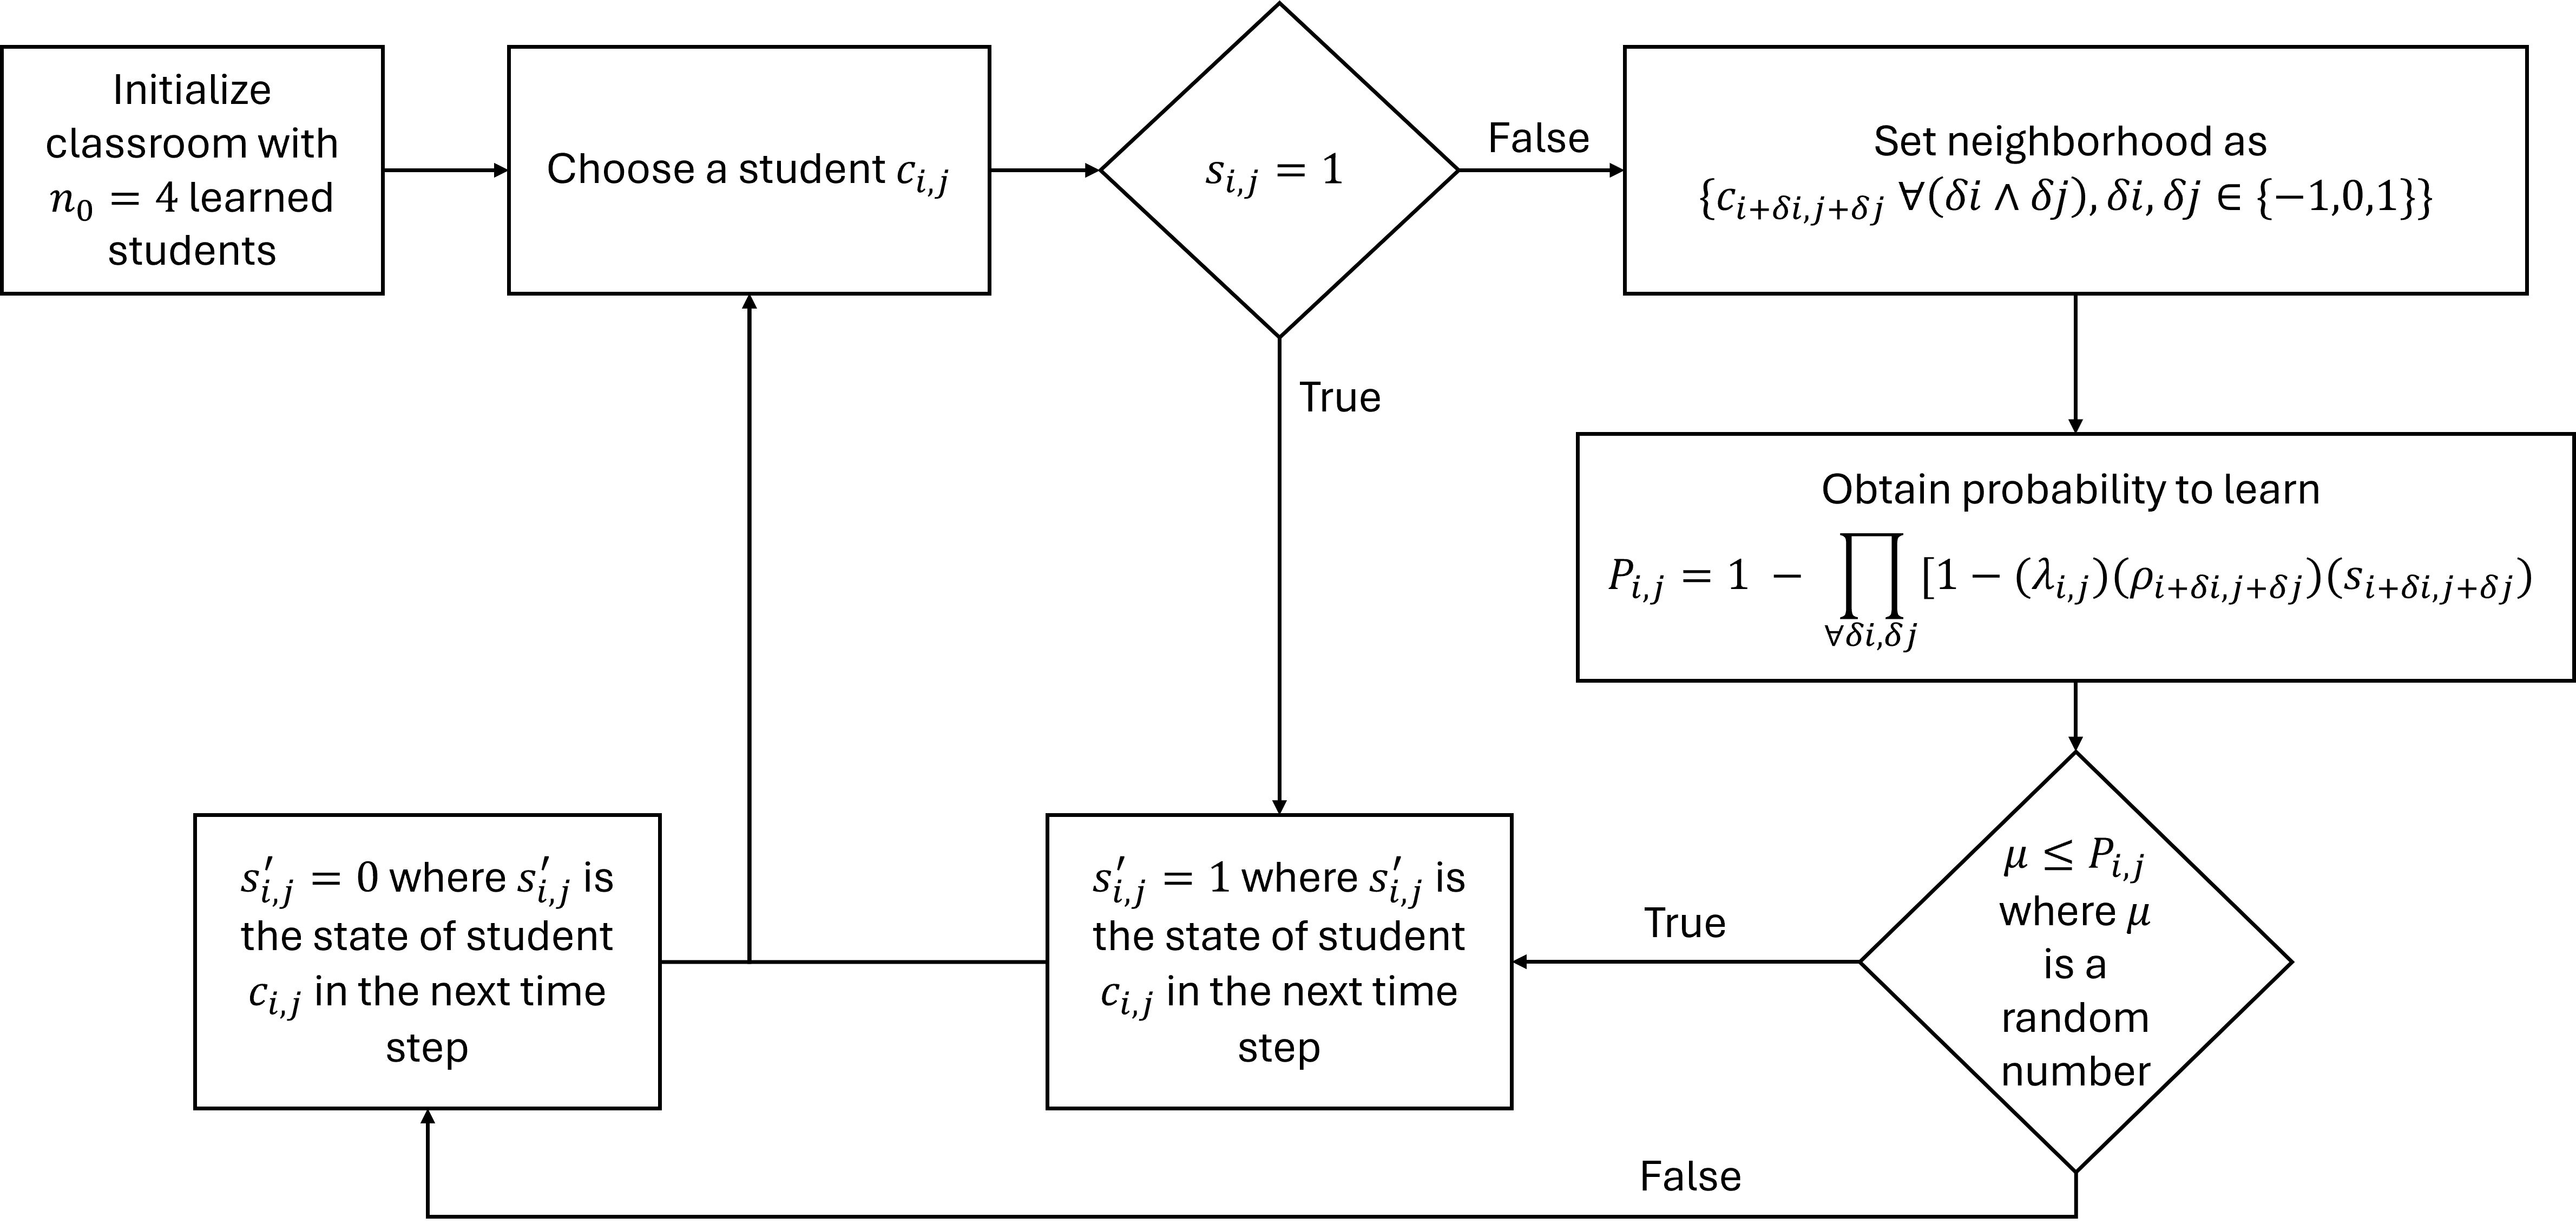
\includegraphics[width=0.8\textwidth]{figures/2DBPCA PI Flowchart.png}
    \caption[Peer instruction flowchart]{Numerical process for simulation of 2D BPCA for PI set-ups.}
    \label{fig:2DBPCA PI Flowchart}
\end{figure}

The seating arrangement (SA) were chosen from a previous study that showed that the SA can affect the learning process \cite{roxas2010seating}. These SA's are namely: inner corner, outer corner, center, and random. The SA configurations are shown in Figure \ref{fig:PI SAs}.

 \begin{figure}[htbp!]
    \centering
    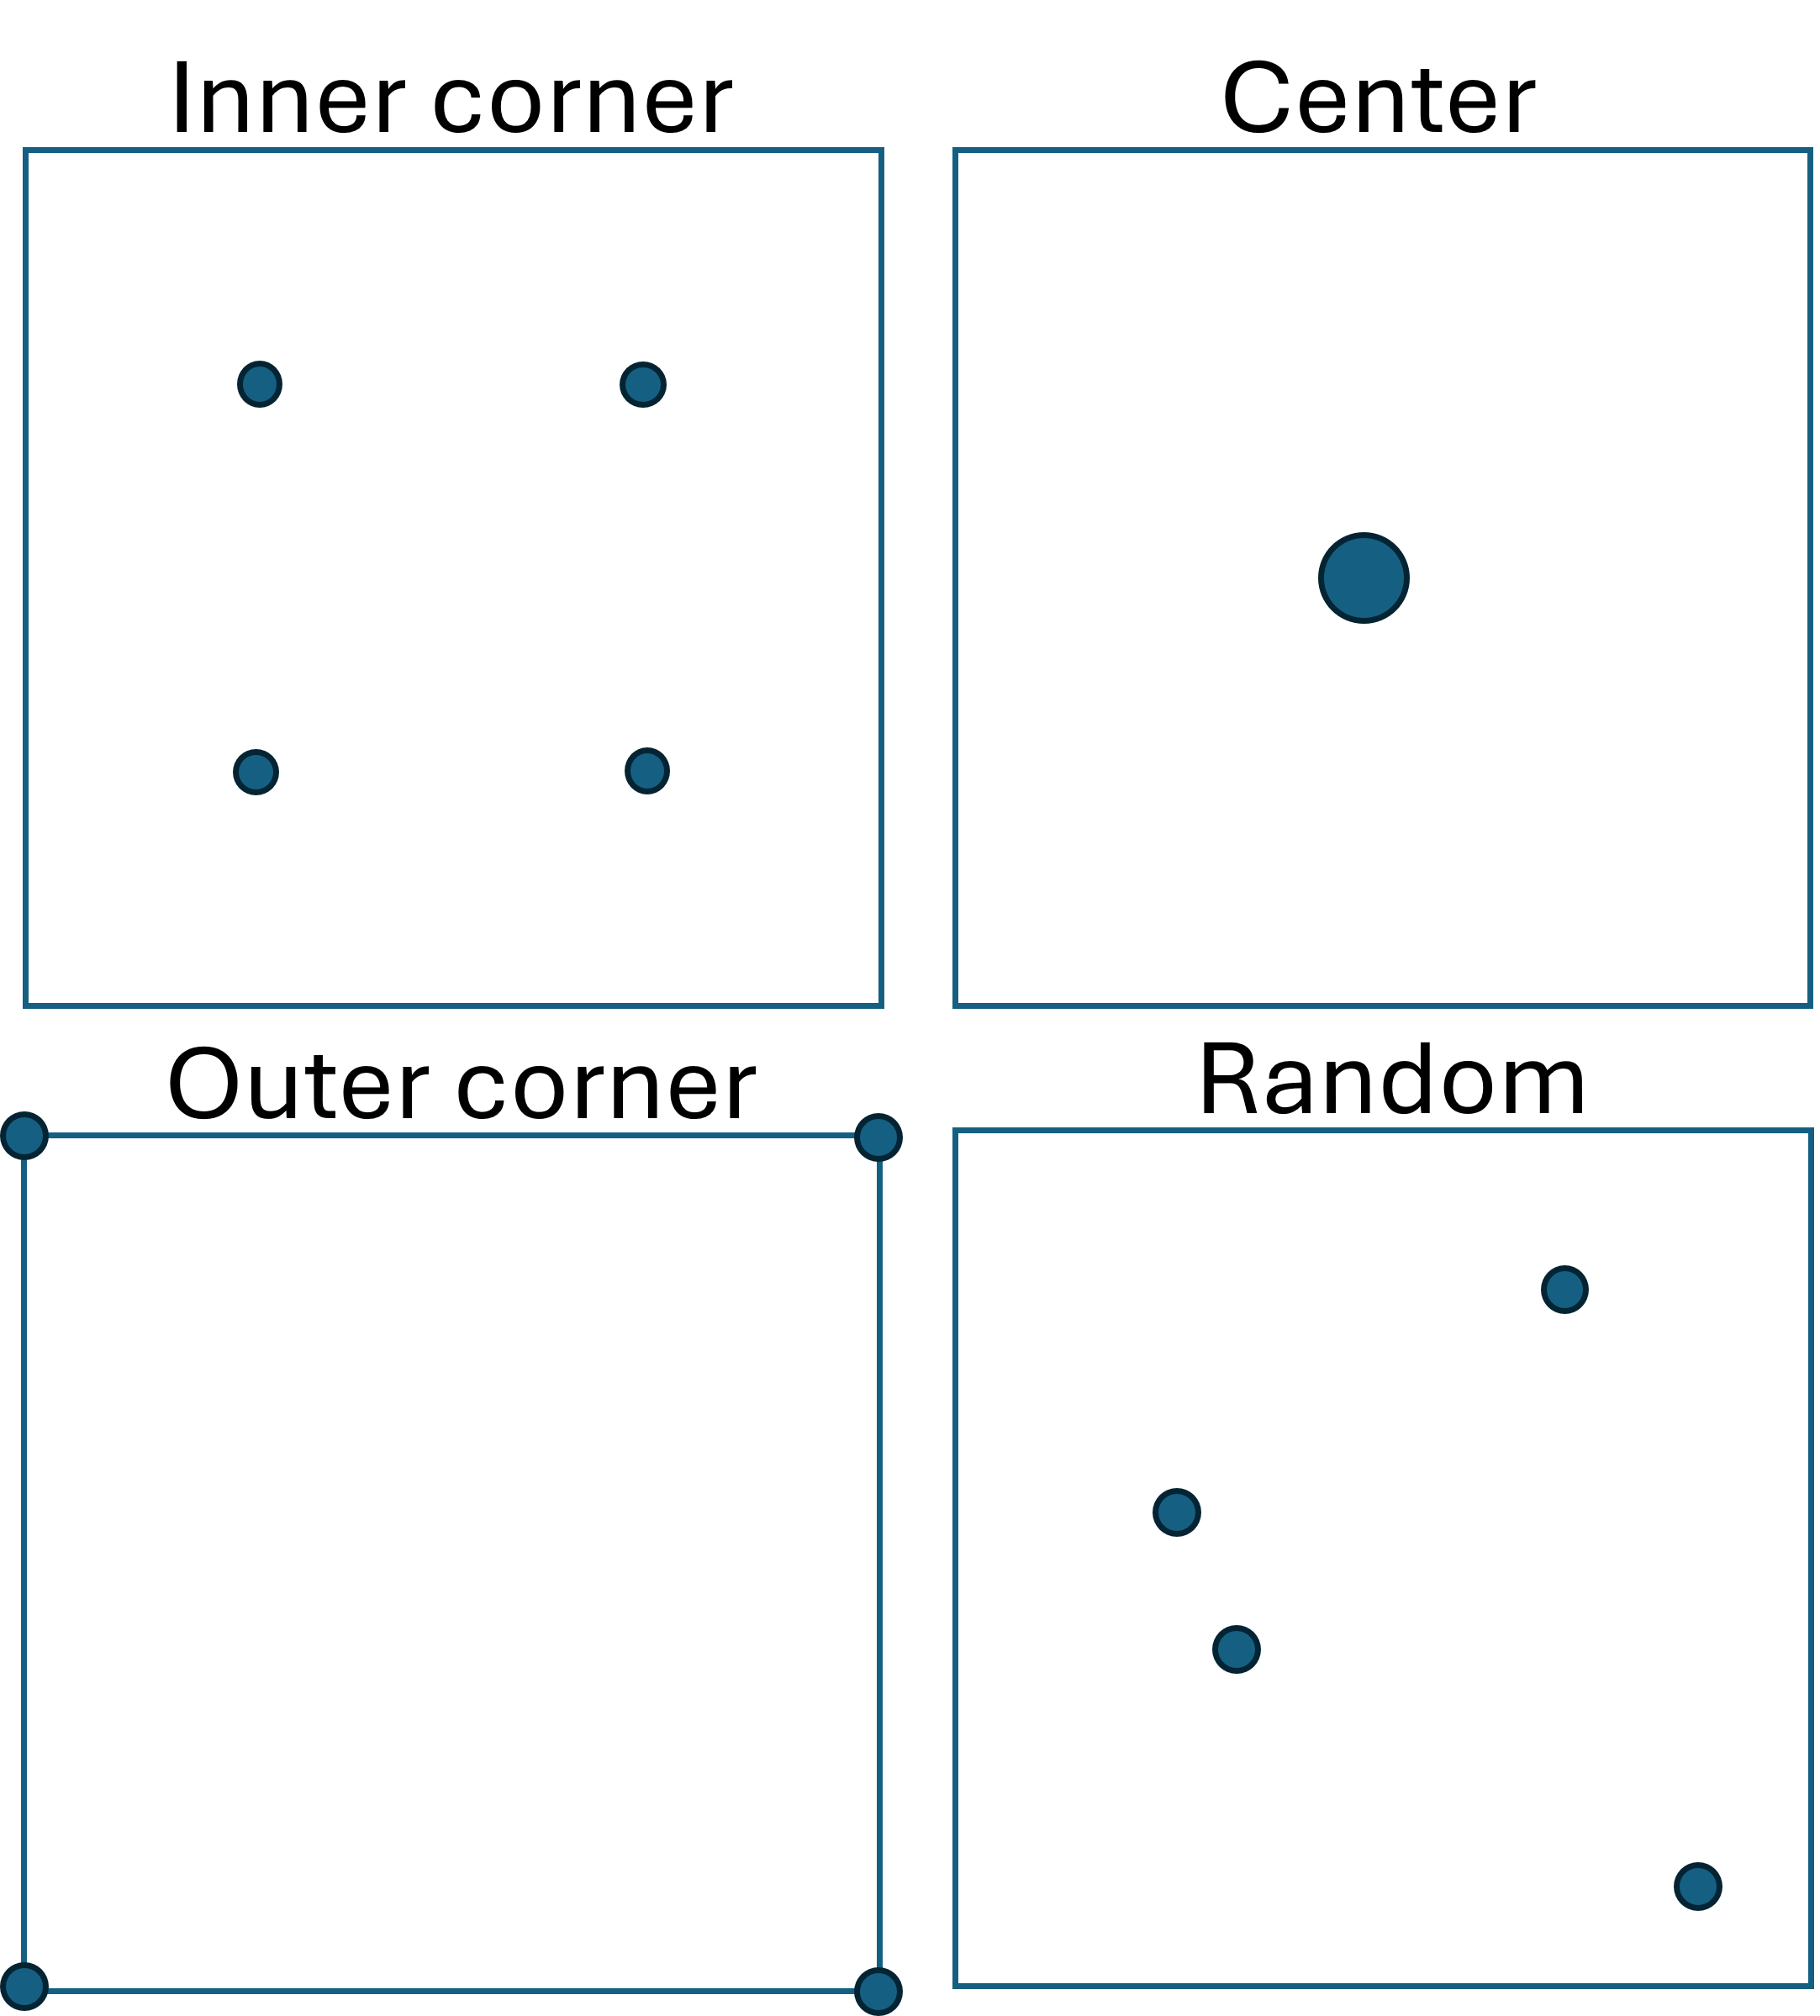
\includegraphics[width=0.5\textwidth]{figures/PI SAs.png}
    \caption[Peer instruction seating arrangements.]{ Peer instruction seating arrangements. Circles denote high aptitude students. The inner corner configuration places high aptitude students halfway between the center and the corner of the classroom. The outer corner configuration places high aptitude students at the corner of the classroom. The center configuration places high aptitude students in the center of the classroom. The random configuration places high aptitude students randomly throughout the classroom.}
    \label{fig:PI SAs}
 \end{figure}

 Figure \ref{fig:Sample classroom evolution} shows an example of classroom's evolution over time. The sample classroom is set with $L=64$, $\lambda_0 = 1$, and $\rho_0 = 0.5$ with the inner corner SA.

 \begin{figure}[htbp!]
    \centering
    \subfigure[$t=1$]{\label{fig:2DBPCA classroom 1}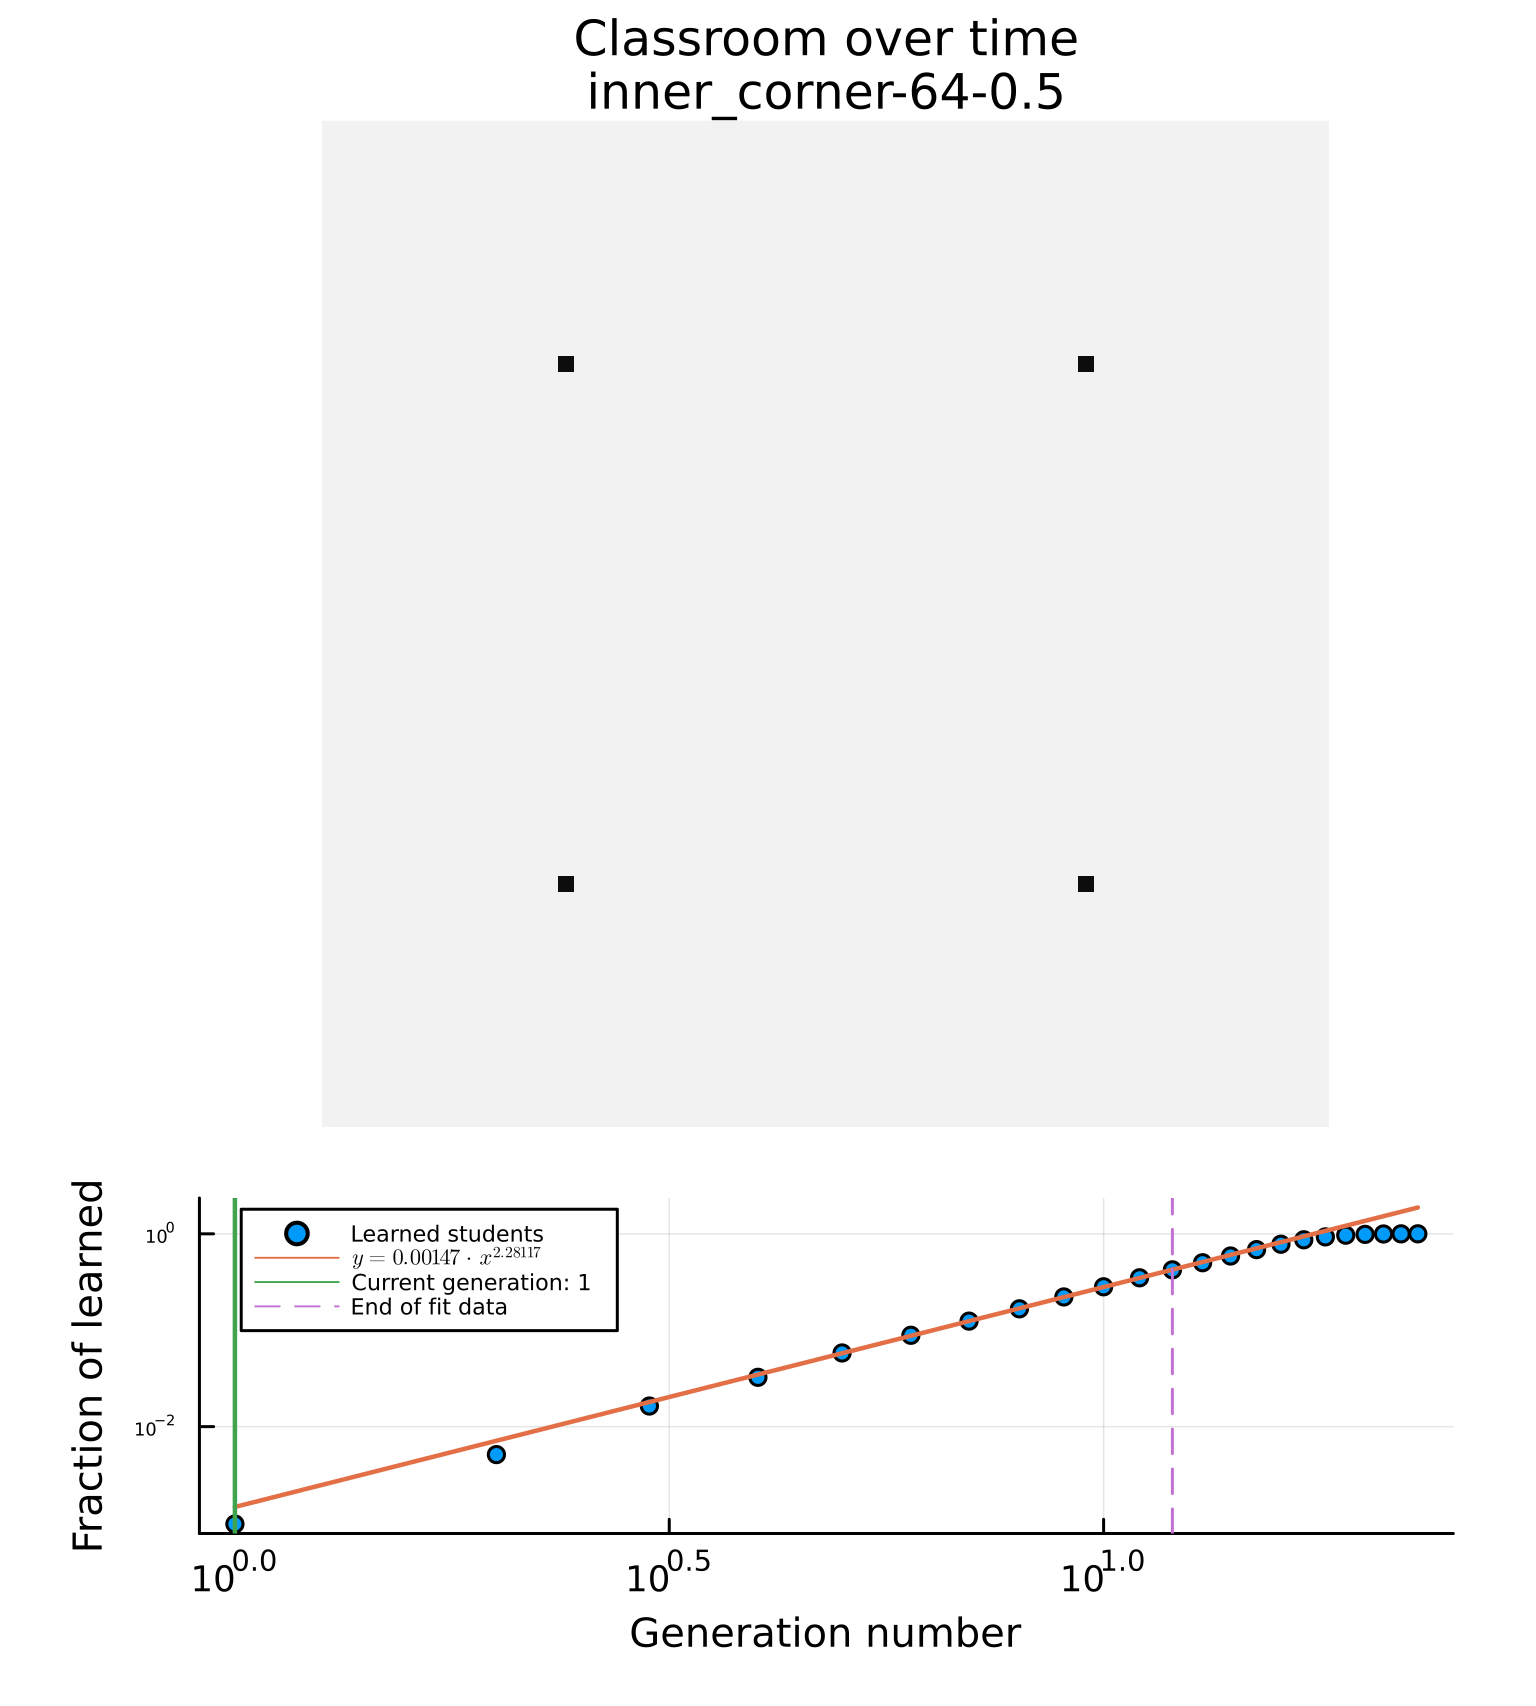
\includegraphics[width=0.45\textwidth]{figures/2D-BPCA-analysis/sample run - PI/2DBPCA-random-64-0.5-1.png}}
    \subfigure[$t=9$]{\label{fig:2DBPCA classroom 9}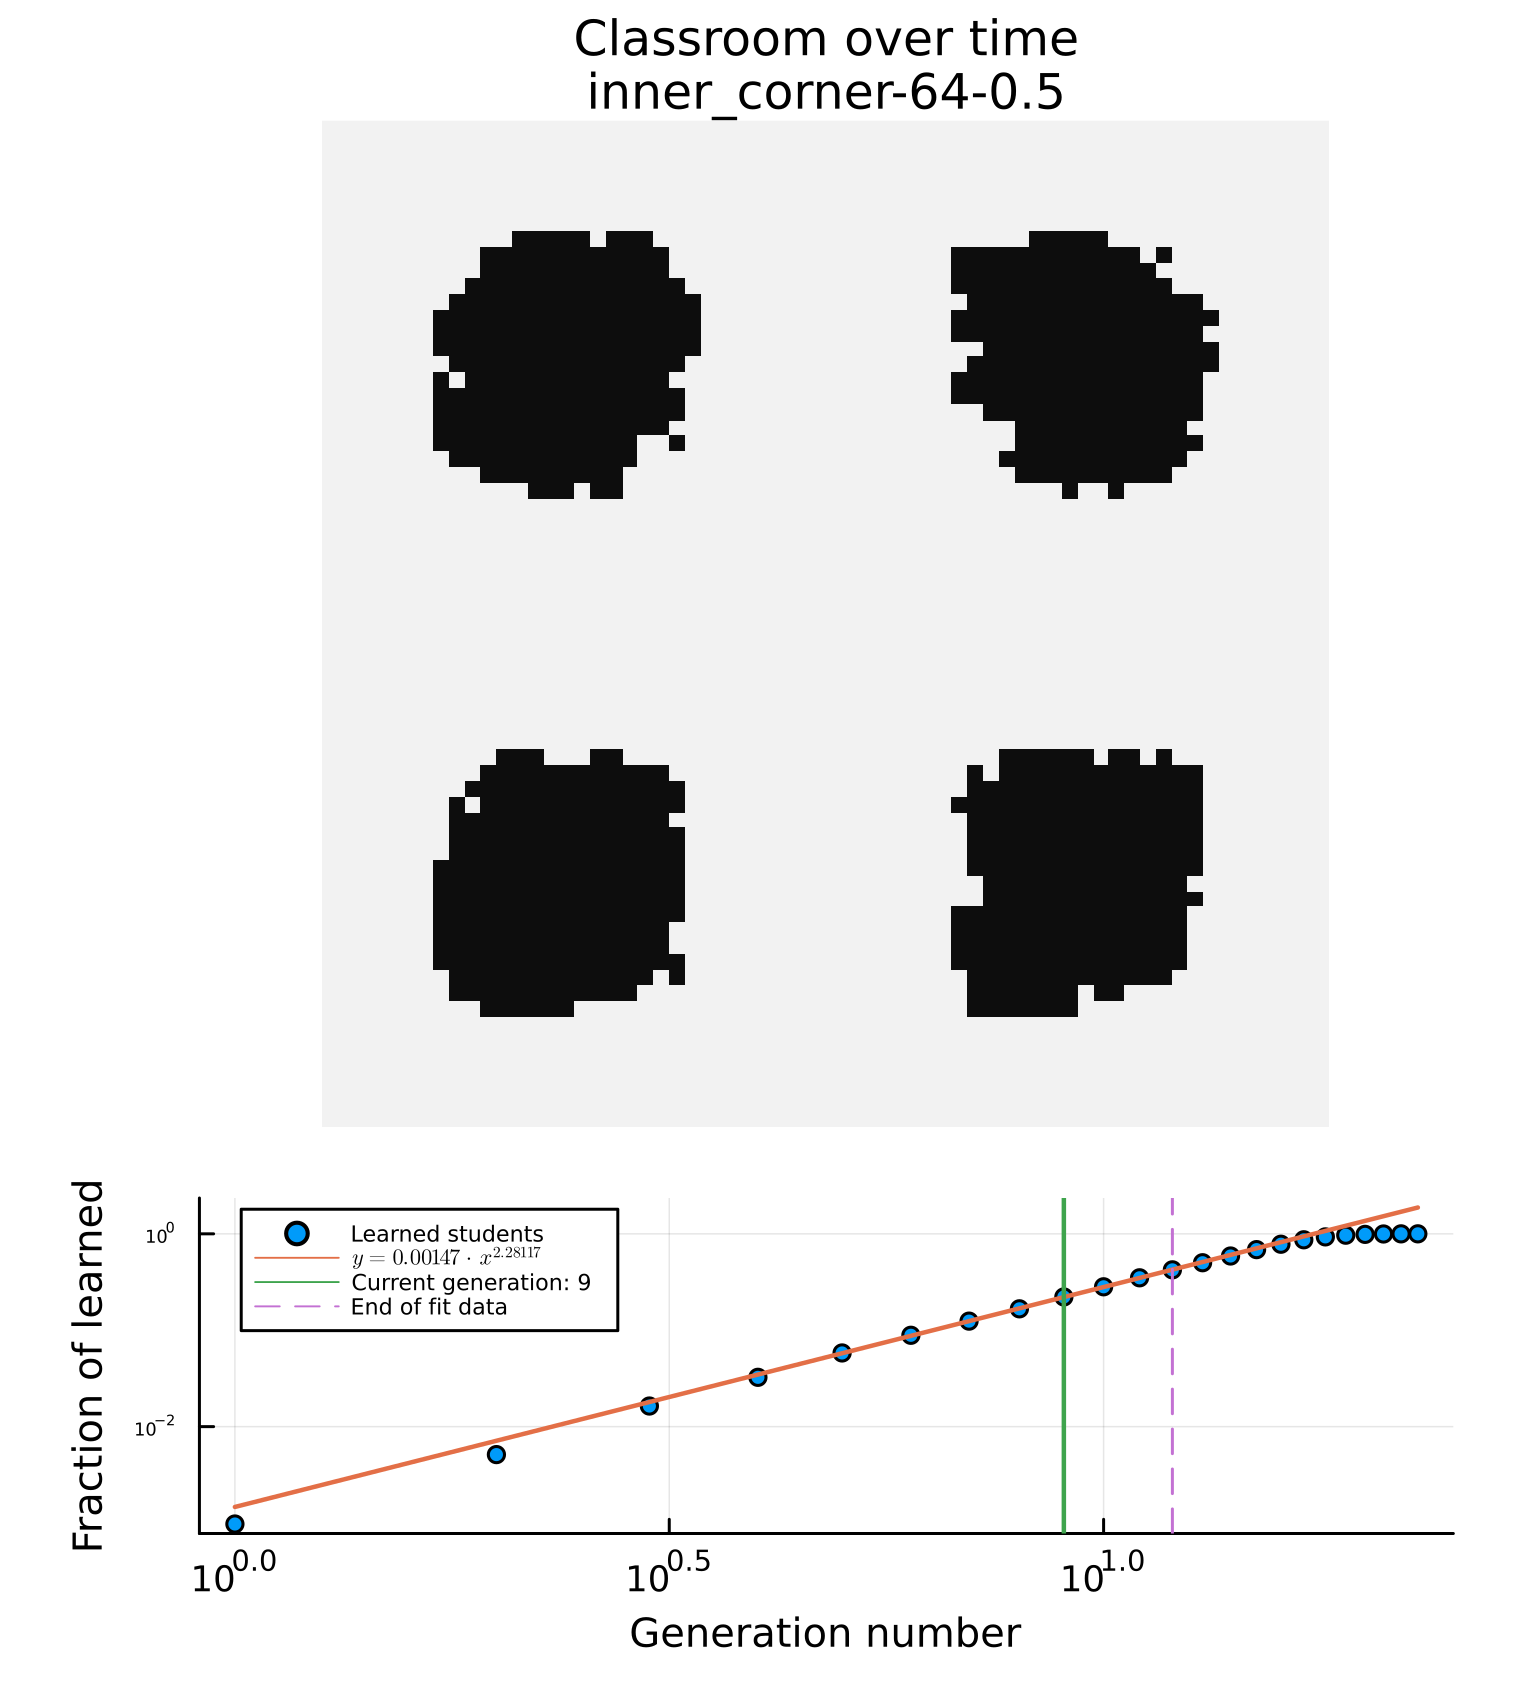
\includegraphics[width=0.45\textwidth]{figures/2D-BPCA-analysis/sample run - PI/2DBPCA-random-64-0.5-9.png}}
    \subfigure[$t=17$]{\label{fig:2DBPCA classroom 17}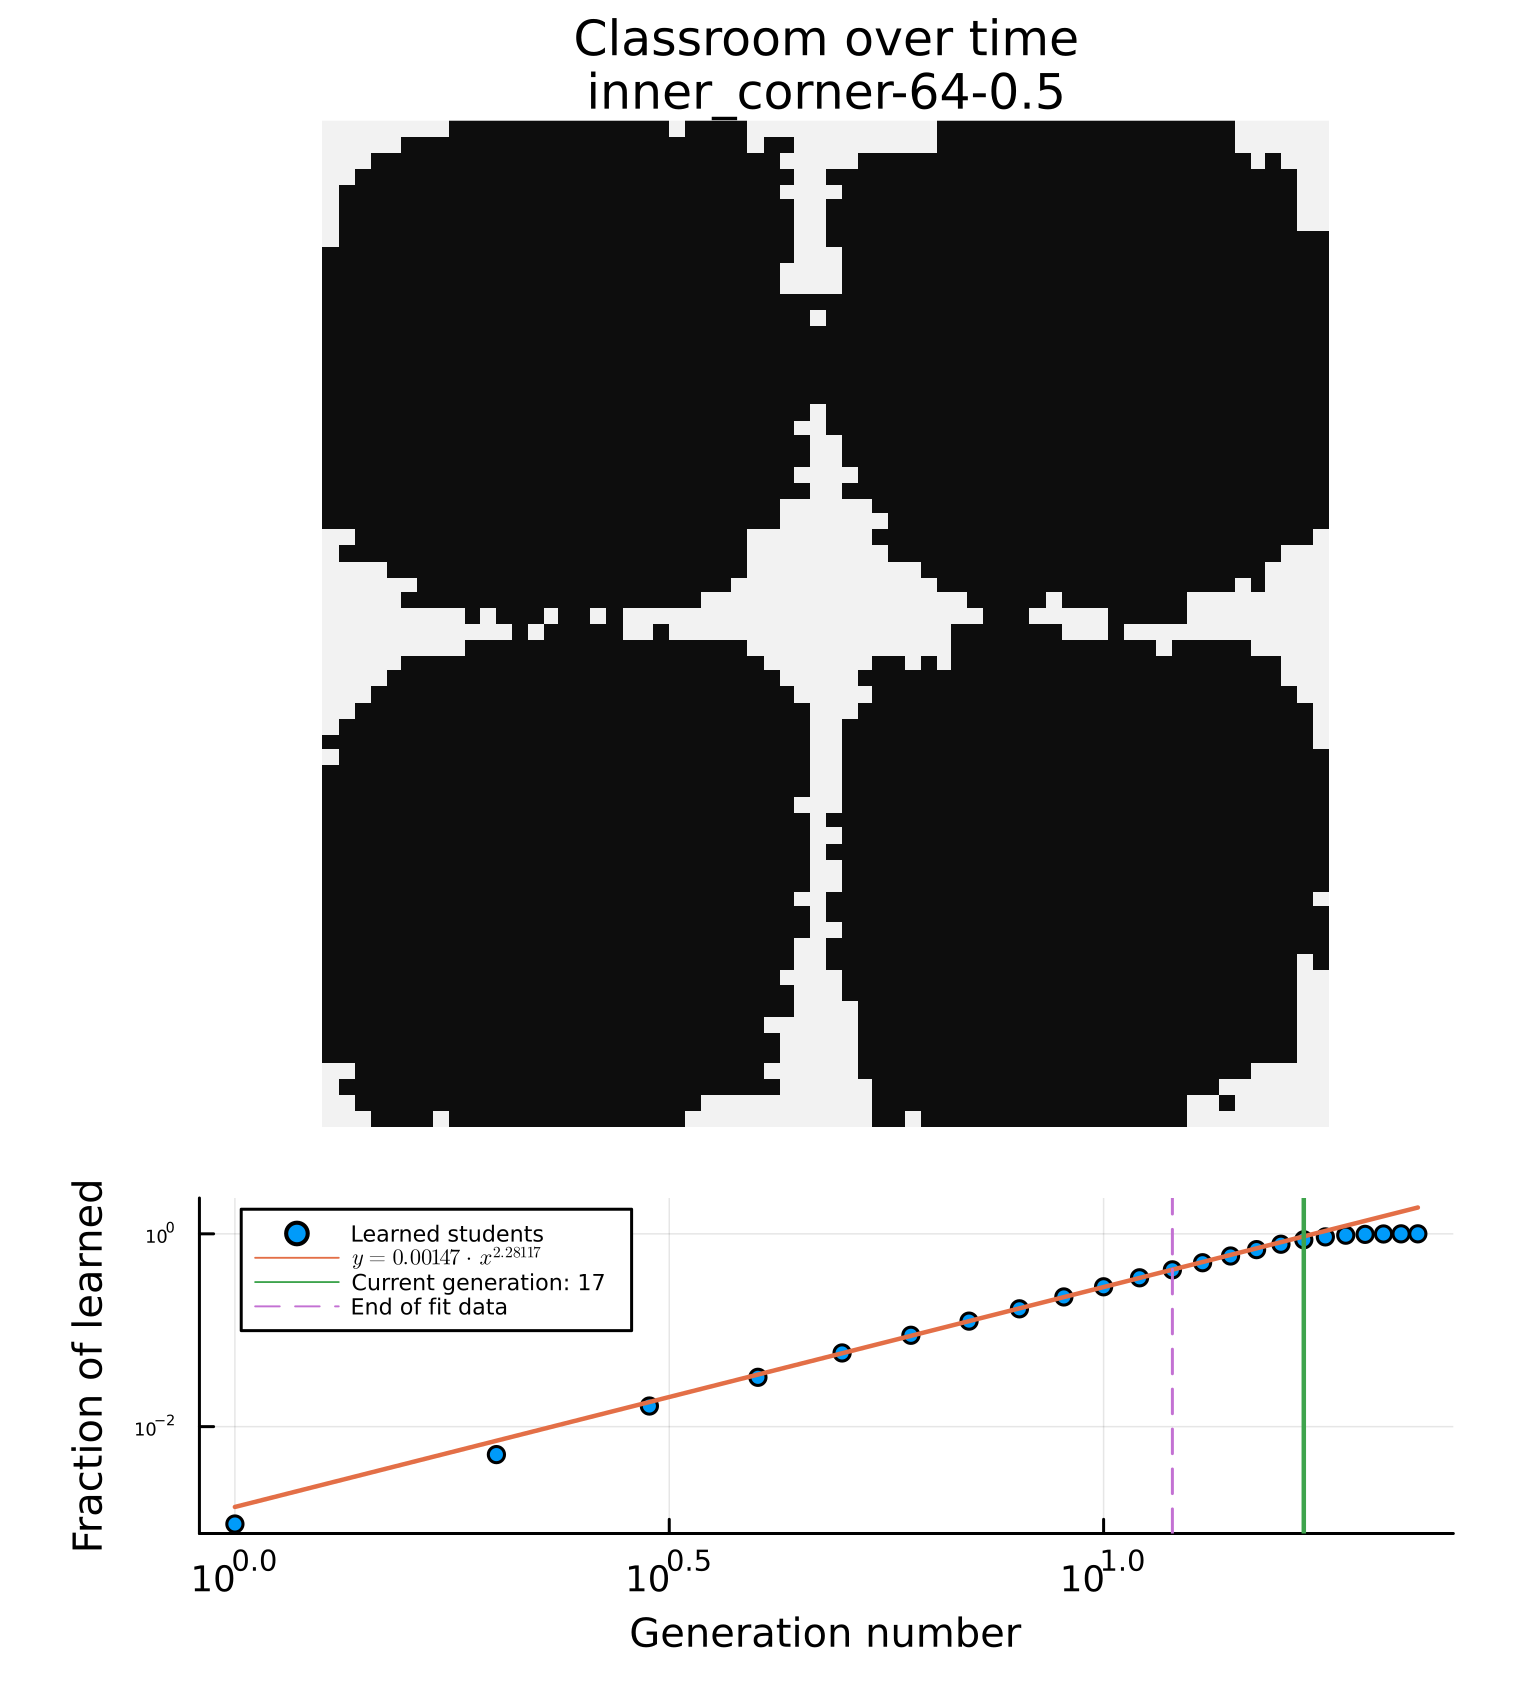
\includegraphics[width=0.45\textwidth]{figures/2D-BPCA-analysis/sample run - PI/2DBPCA-random-64-0.5-17.png}}
    \subfigure[$t=23$]{\label{fig:2DBPCA classroom 1}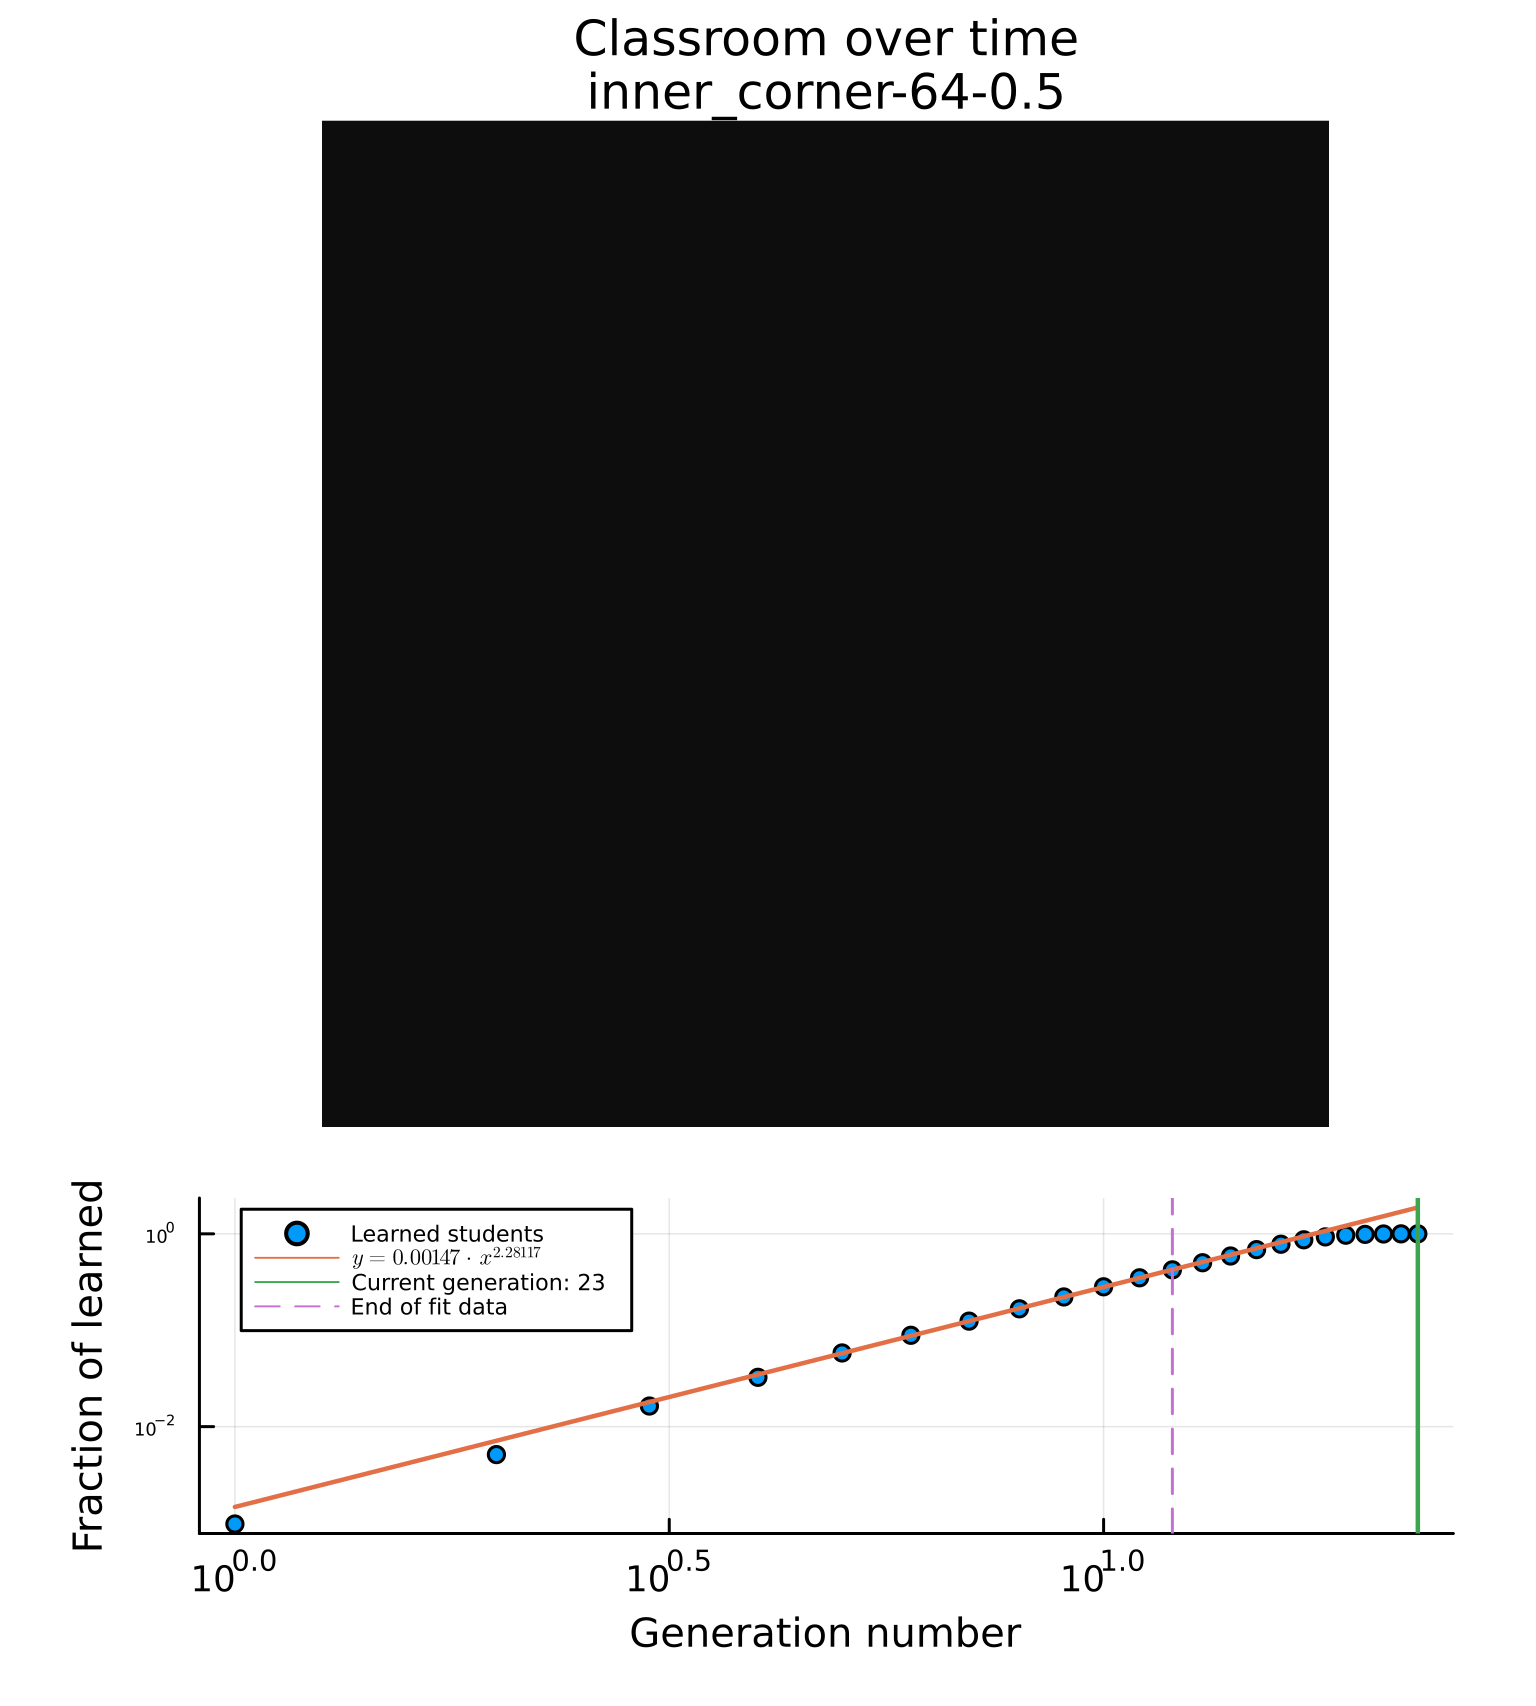
\includegraphics[width=0.45\textwidth]{figures/2D-BPCA-analysis/sample run - PI/2DBPCA-random-64-0.5-23.png}}
    \caption{Sample classroom evolution for $L=64$, $\lambda_0 = 1$, and $\rho_0 = 0.5$ with the inner corner SA. Black squares represent learned students while white squares represent unlearned students. The accompanying graphs show the fraction of learned students as a function of time. The blue circle represents the data points while the orange line shows the power law fit. The broken pink line shows the where we truncate the data for fitting the power law and the green line shows the current time step in the plot.}
    \label{fig:Sample classroom evolution}
 \end{figure}

\section{The binary probabilistic cellular automata model for a traditional classroom set up}
The main difference between the PI model and the traditional instructional model is that the latter only relies on one source of information - the teacher. To simulate this, for each time step, we set the probability of each student to learn $P_{ij}$ to be the product of their individual learning rate $\lambda_{i,j}$ and probability of learning from the teacher $\rho_{0}$. 
\begin{equation}
    \label{eq:BPCA traditional learning probability}
        P_{ij} = \lambda_{ij} \rho_{0}
\end{equation}
The five-tuple of the traditional instructional model then only differs from the PI model in the update rule $\mathcal{R}$.

The numerical procedure is outlined in Figure \ref{fig:2DBPCA Traditional Flowchart}. Each simulation for the traditional model starts with all students unlearned. Similar with the PI model, the simulation is considered finished once all the students have learned.

\begin{figure}[htbp!]
    \centering
    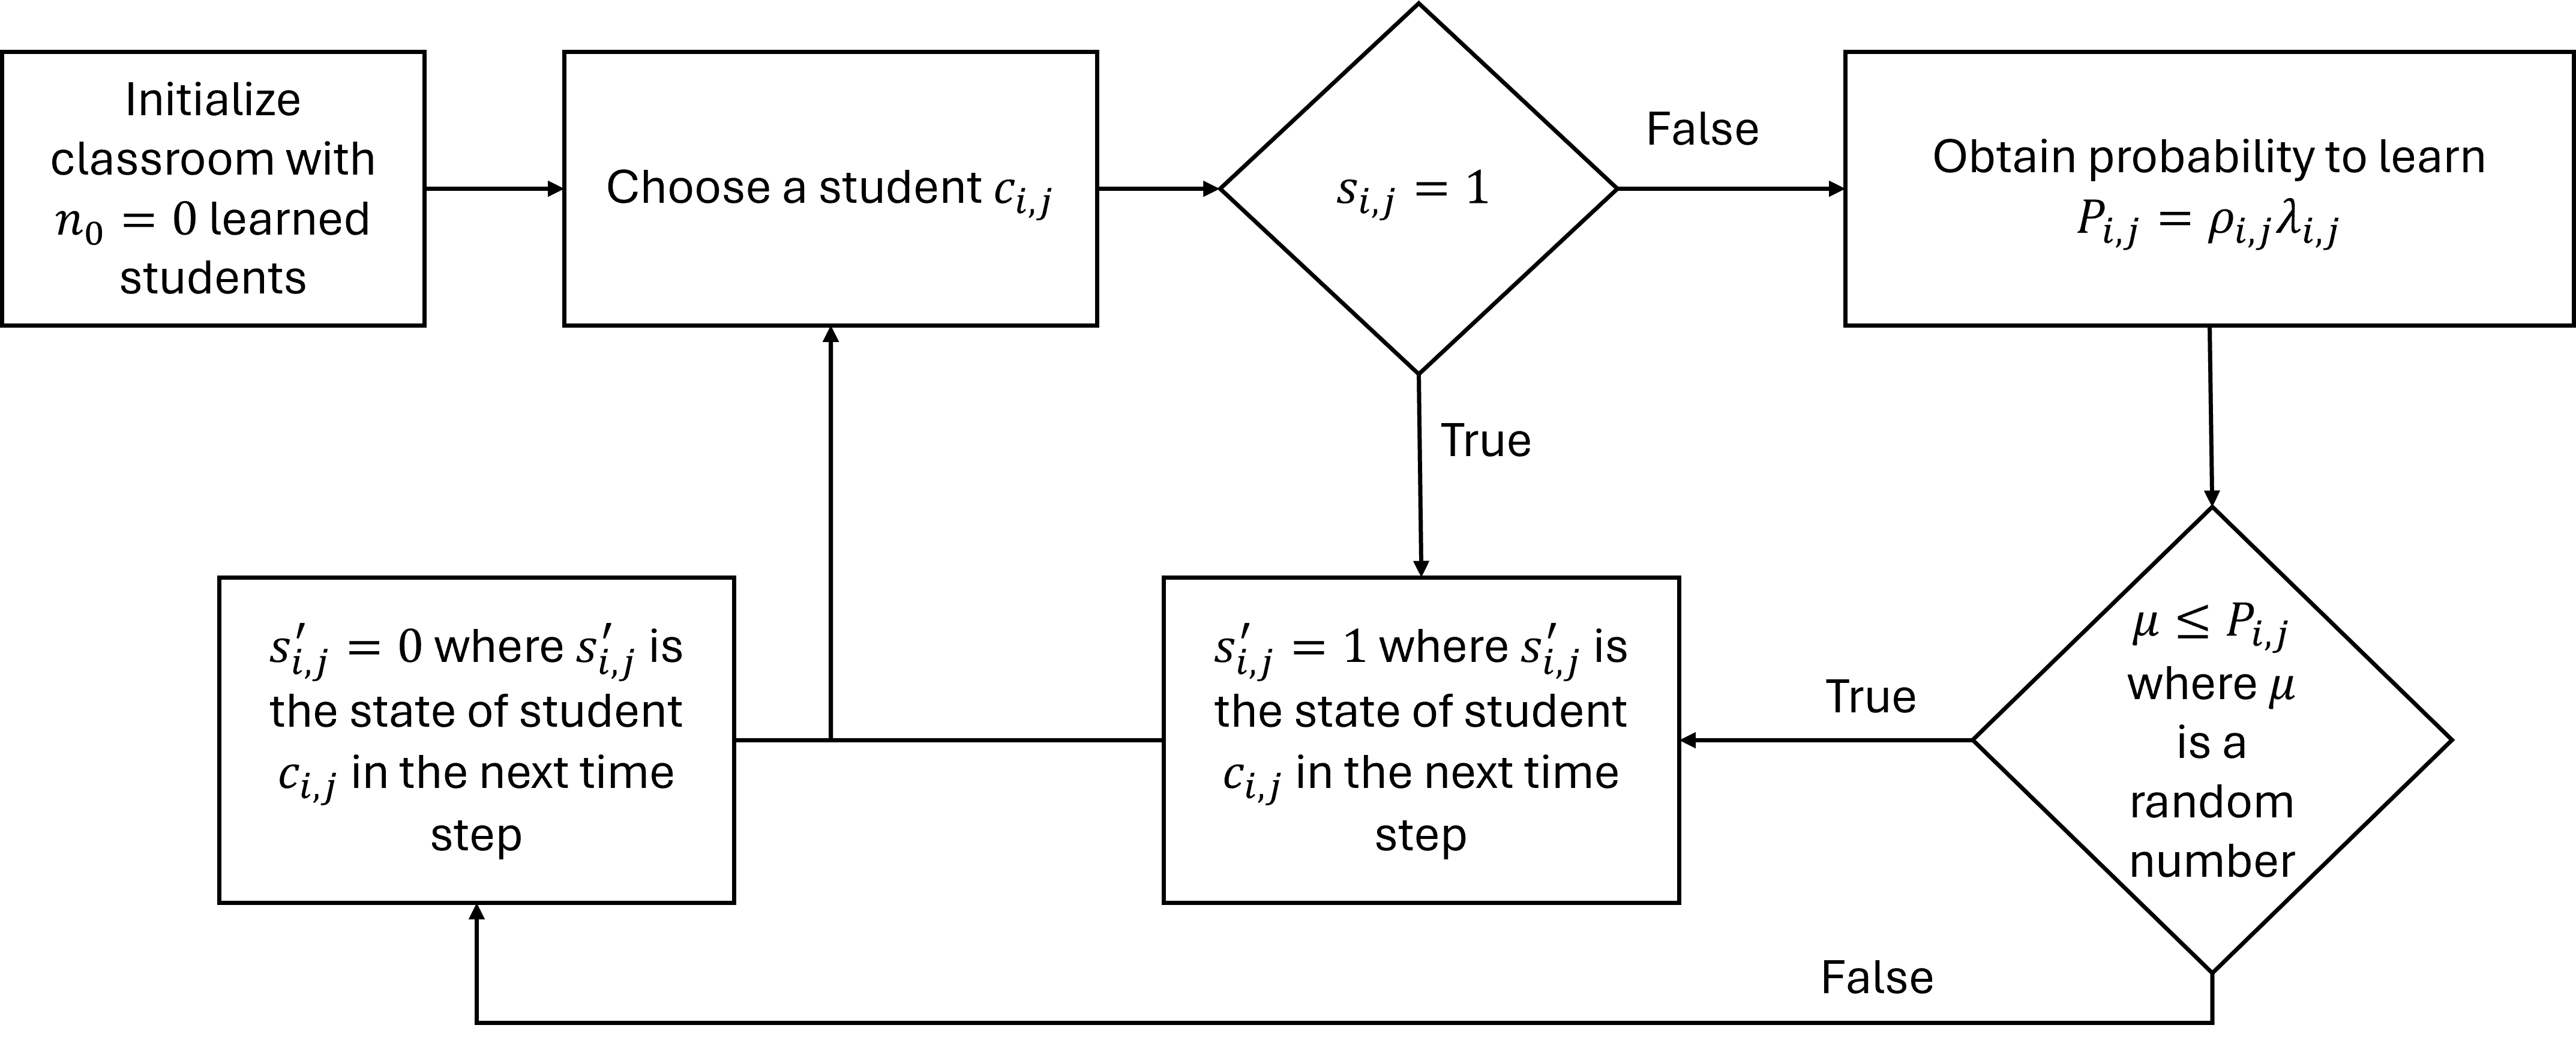
\includegraphics[width=0.8\textwidth]{figures/2DBPCA TI Flowchart.png}
    \caption[Traditional instruction flowchart]{Numerical process for simulation of 2D BPCA for traditional set-ups.}
    \label{fig:2DBPCA Traditional Flowchart}
\end{figure}

\section{Results: Homogenous PI vs Traditional}
In this chapter, we only consider the case where all students have the same learning rate $\lambda_{i,j} = \lambda_0 = 1$ and an isotropic positional learning factor $\rho_{i,j} = \rho_0 \space ~\forall~ (\delta i \land \delta j),  \delta i, \delta j \in \lbrace -1,0,1 \rbrace $. From the simulations, we compared both the average number time steps $\langle t_{max} \rangle$ it takes for all the students in the classroom to learn and the average learning rate $\langle m \rangle$ across different configurations over 5 independent runs. The learning rate $m$ for each trial was obtained by using a Levenberg-Marquardt algorithm to fit a power law ($y = ax^m$) to the fraction of learned students as a function of the generation number. We only considered the first $50\%$ of the data for the PI model or the first $25\%$ of the data for the traditional model. This truncation was done so that we only fit the part of the data before the finite size effect starts to affect the simulation.

\subsection{Time to learn $t_{max}$ vs positional learning factor $\rho_0$} \label{subsec: 2DBPCA tmax vs rho}

The data in Figure \ref{fig:2DBPCA tmax vs rho} shows that the time to learn $t_{max}$ decreases with increasing positional learning factor $\rho_0$ for all classroom sizes for both traditional models and PI models. Among PI models, the inner corner configuration has the lowest $t_{max}$ for all classroom sizes. The outer corner and center SAs performed similarly, while the random SA has the highest $t_{max}$. The traditional model performs situationally better than even the inner corner PI model, something we will investigate in Section \ref{subsec: 2DBPCA tmax vs N}.

\begin{figure}[htbp!]
    \centering
    \subfigure[$L=32$]{\label{fig:2DBPCA tmax vs rho 32}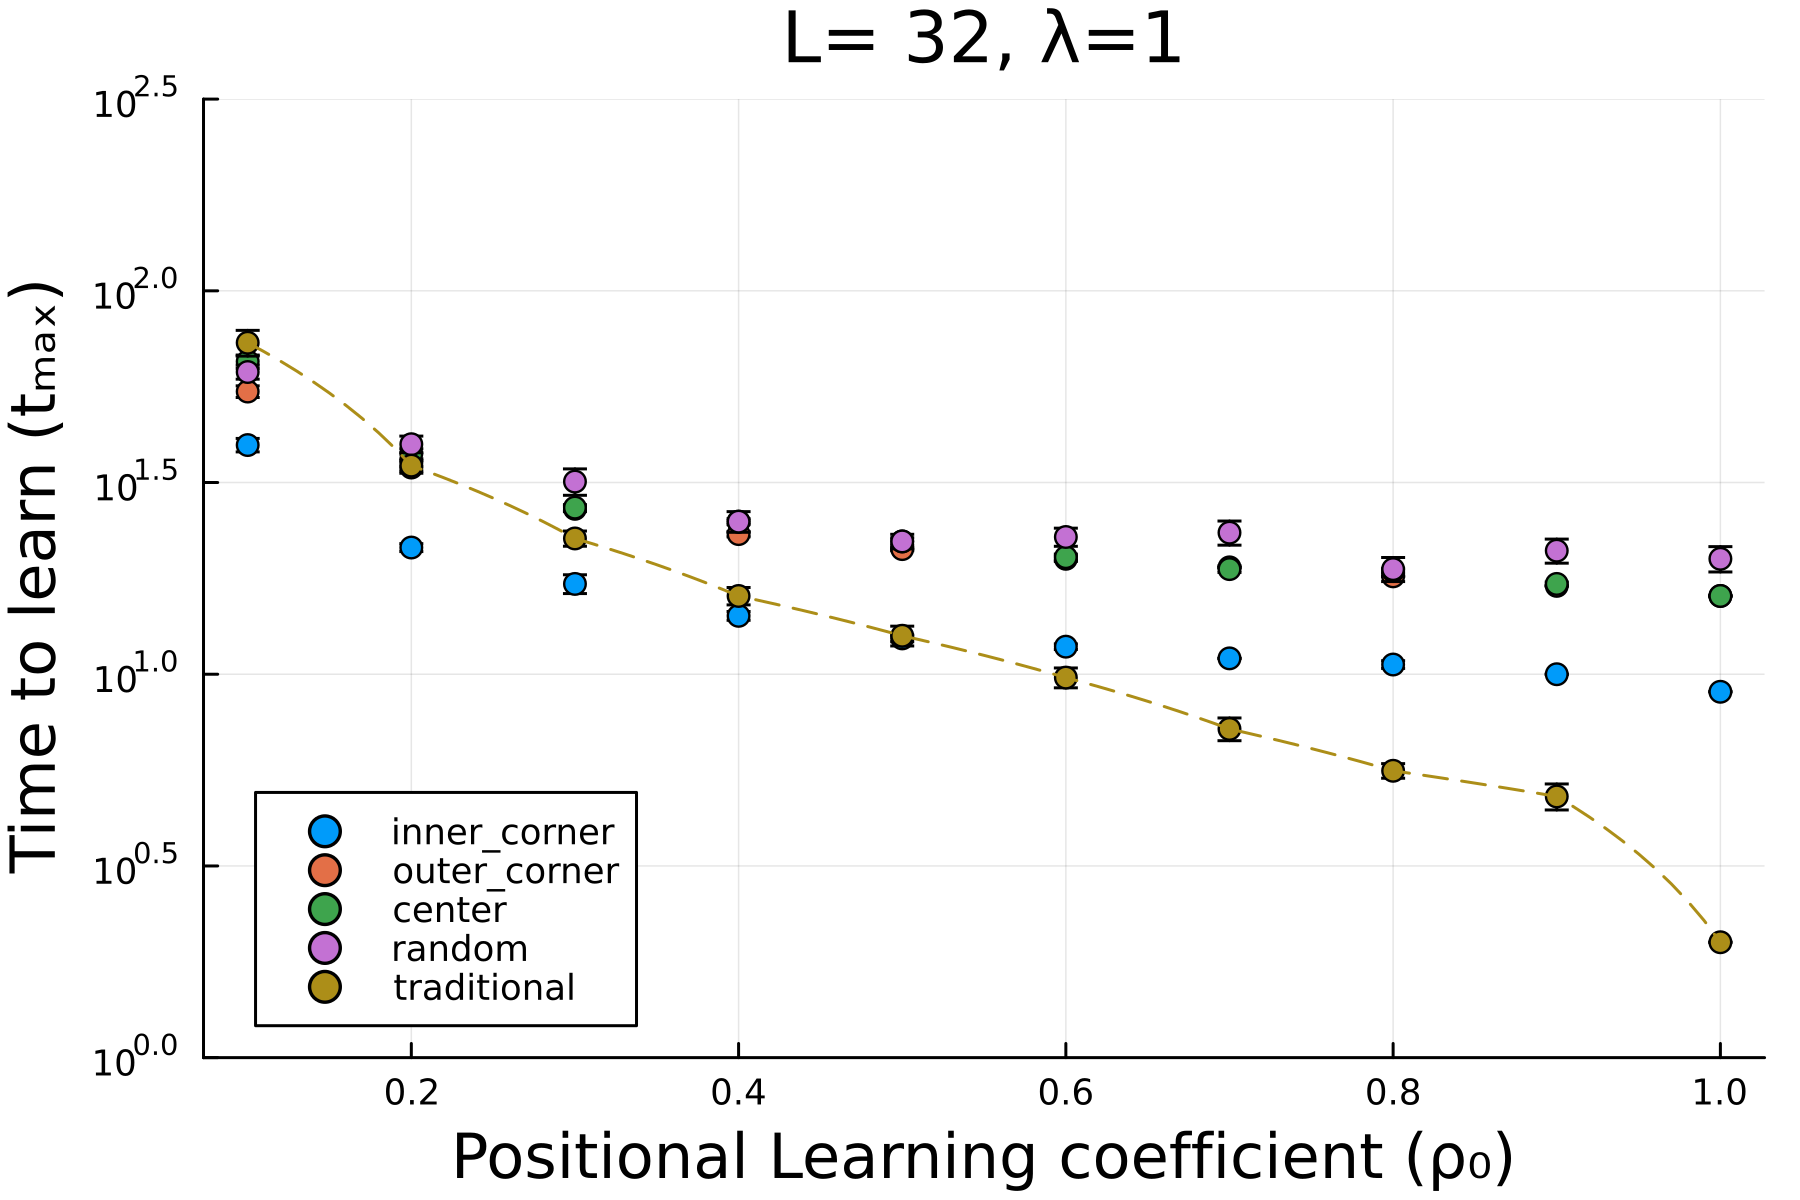
\includegraphics[width=0.45\textwidth]{figures/2D-BPCA-analysis/t-32.png}}
    \subfigure[$L=48$]{\label{fig:2DBPCA tmax vs rho 48}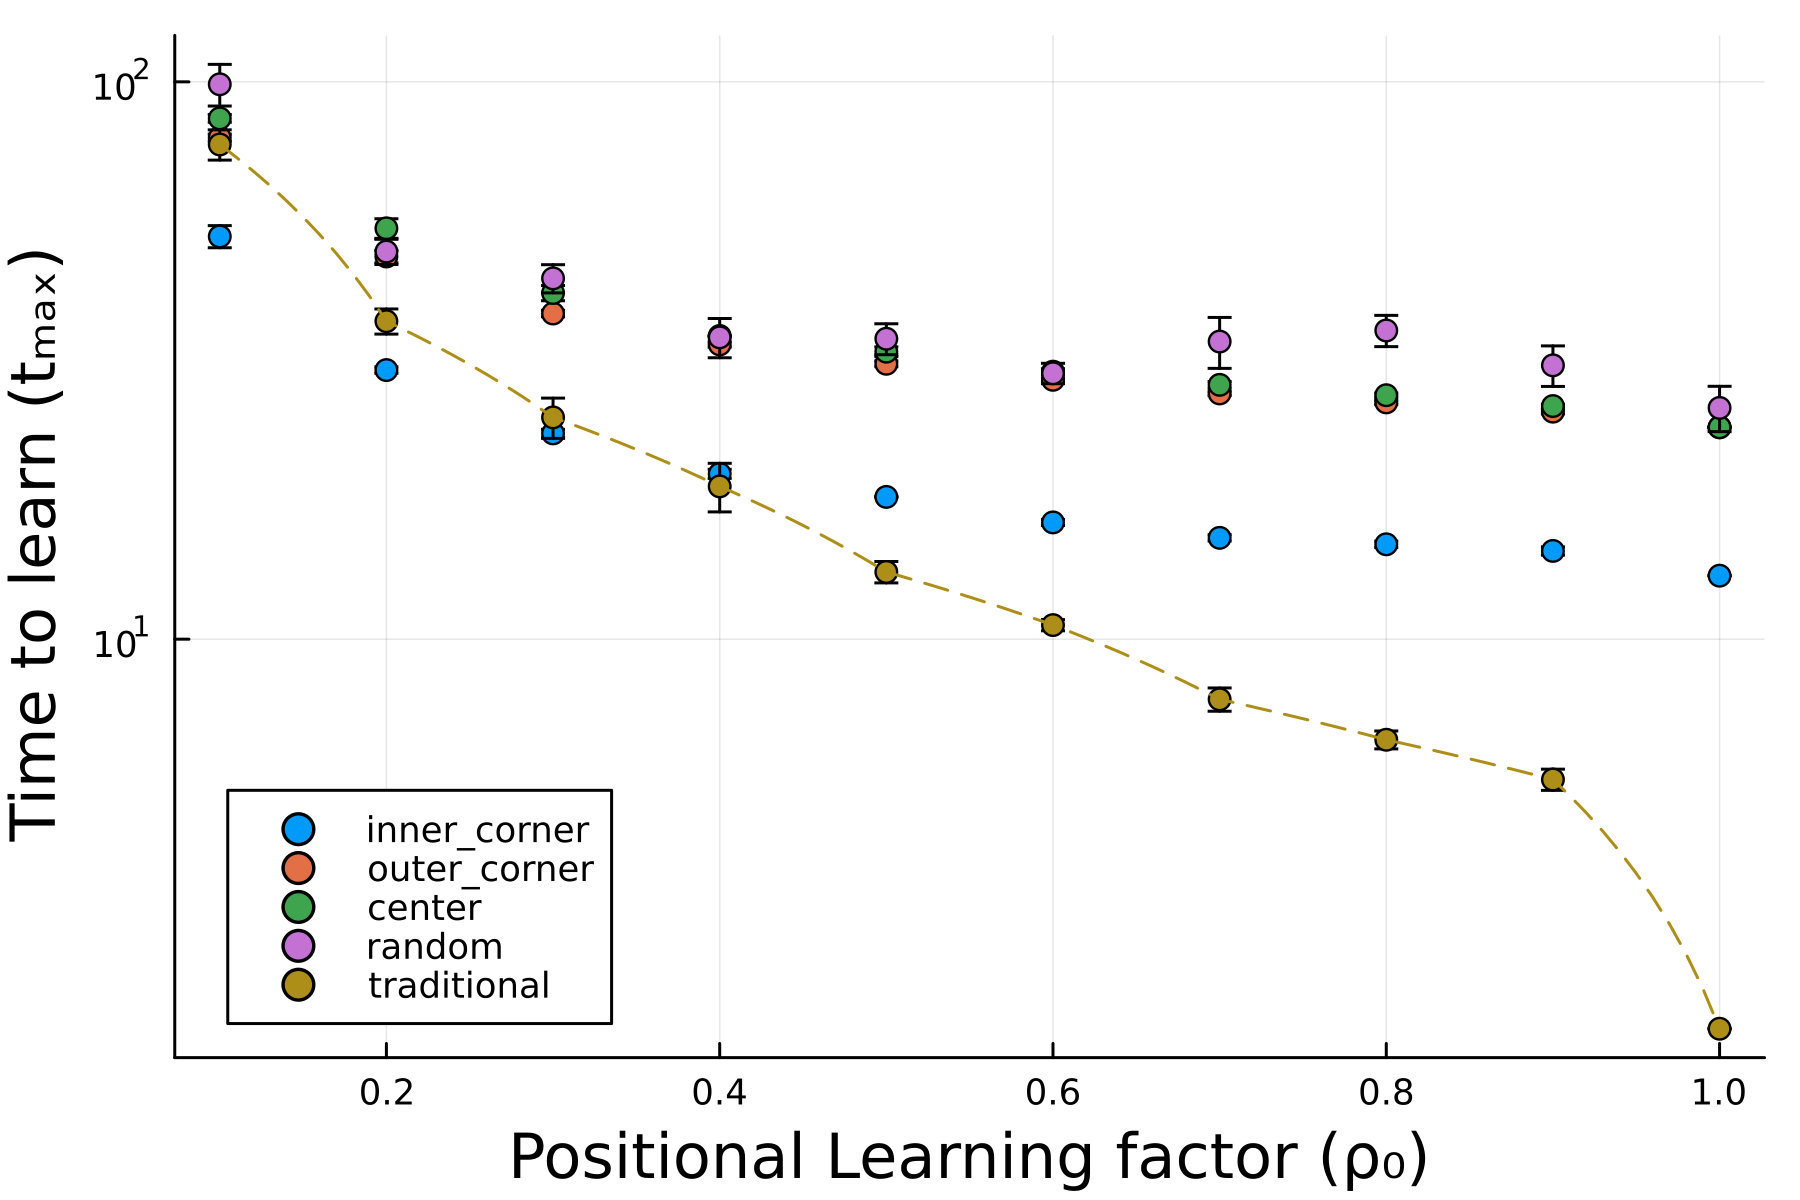
\includegraphics[width=0.45\textwidth]{figures/2D-BPCA-analysis/t-48.png}}
    \subfigure[$L=64$]{\label{fig:2DBPCA tmax vs rho 64}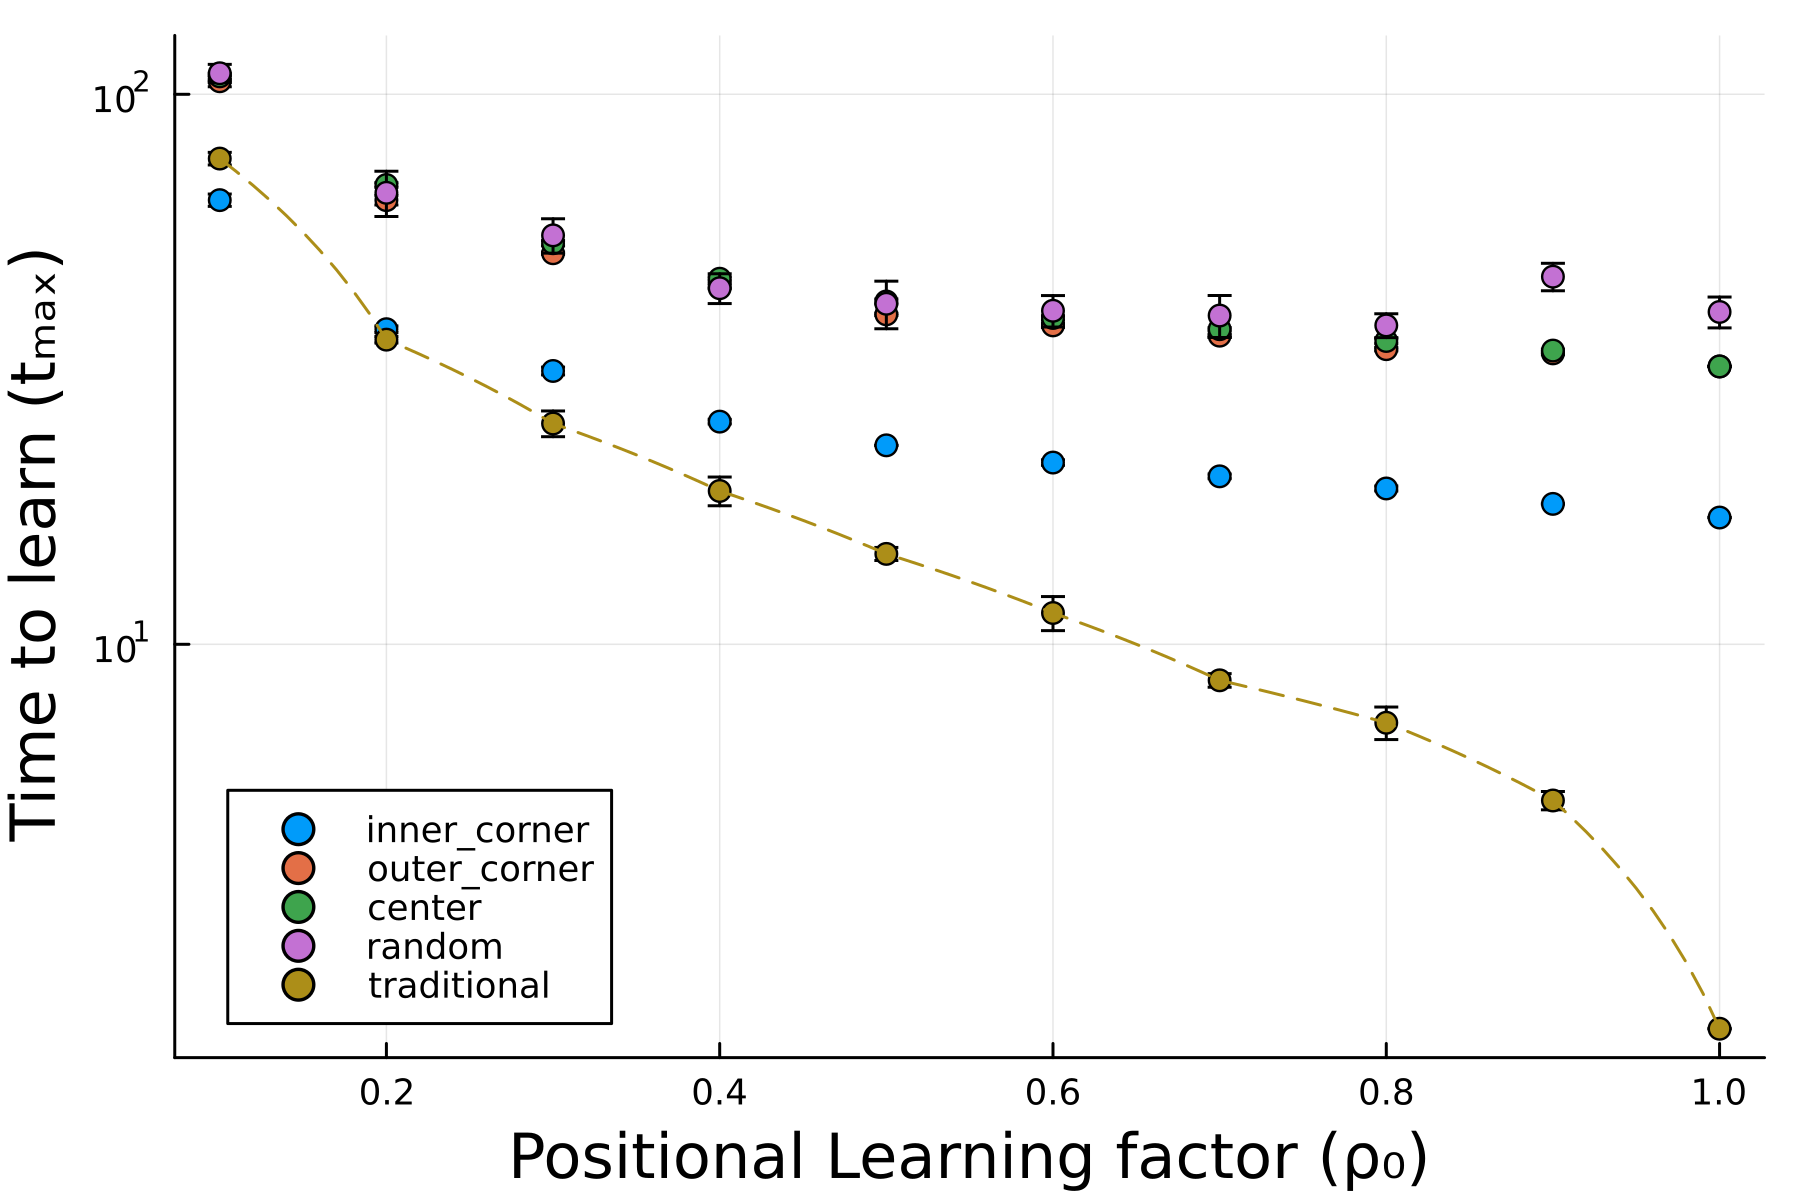
\includegraphics[width=0.45\textwidth]{figures/2D-BPCA-analysis/t-64.png}}
    \subfigure[$L=96$]{\label{fig:2DBPCA tmax vs rho 96}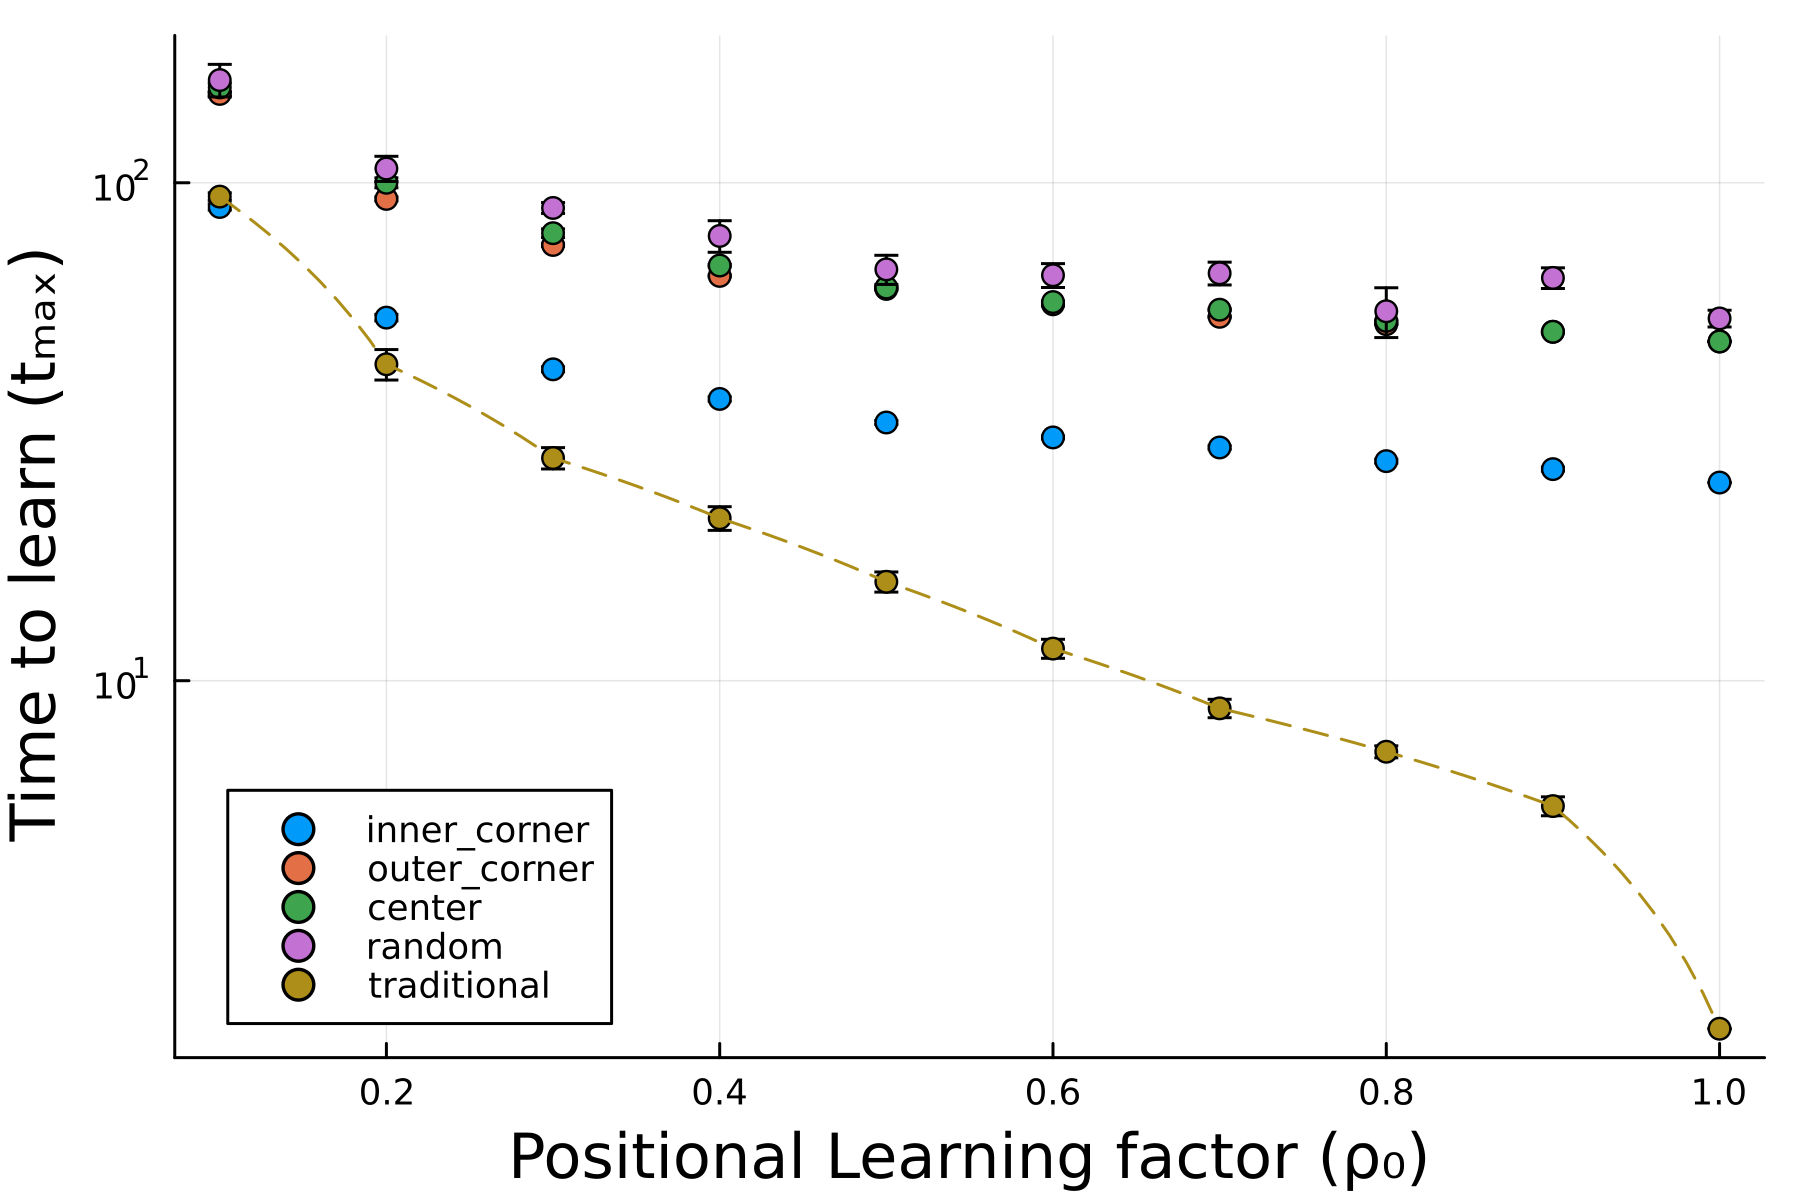
\includegraphics[width=0.45\textwidth]{figures/2D-BPCA-analysis/t-96.png}}
    \subfigure[$L=128$]{\label{fig:2DBPCA tmax vs rho 128}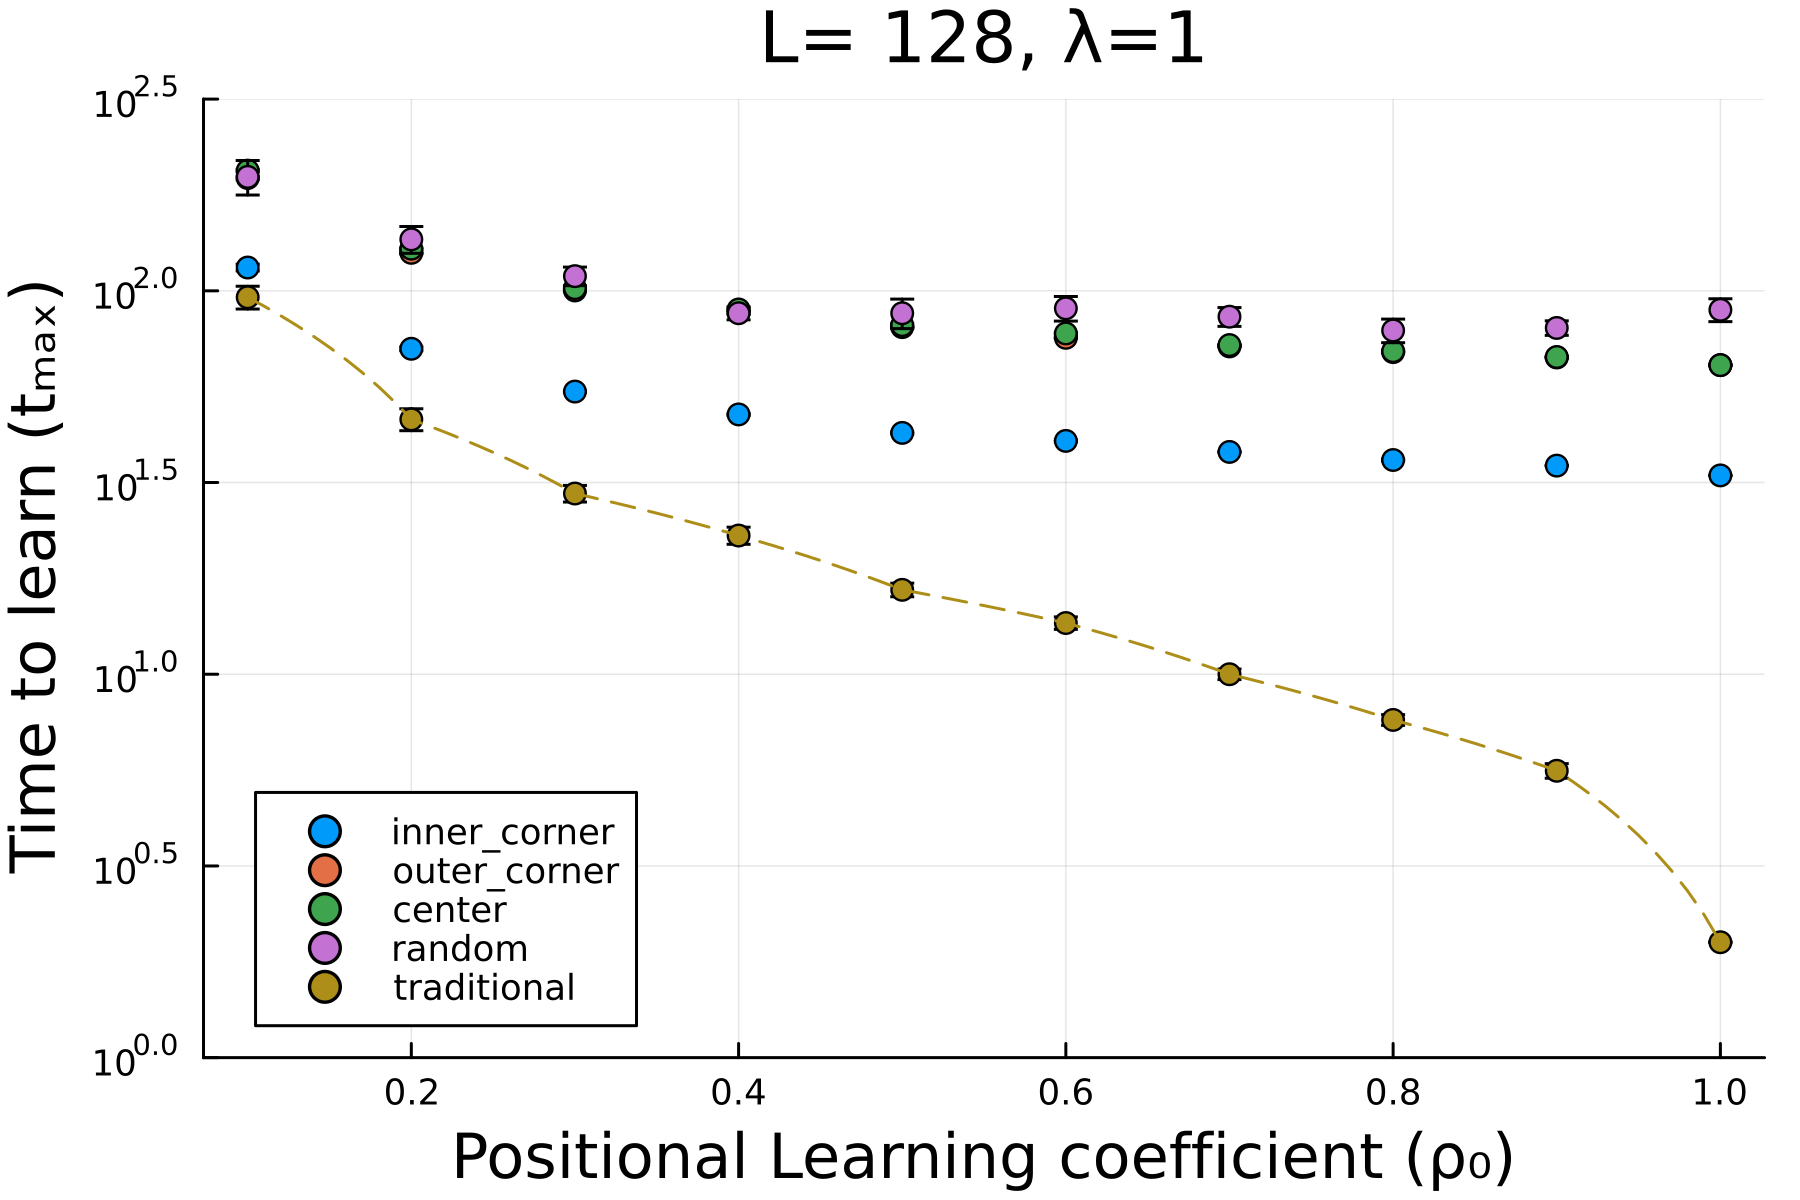
\includegraphics[width=0.45\textwidth]{figures/2D-BPCA-analysis/t-128.png}}
    \caption{Time to learn $t_{max}$ as a function of positional learning factor $\rho_0$ for different classroom sizes $L \in \lbrace 32,48,64,96,128 \rbrace$. Lower time to learn $t_{max}$ indicate better performance.}
    \label{fig:2DBPCA tmax vs rho}
\end{figure}

\newpage

\subsection{Learning rate $m$ vs positional learning factor $\rho_0$}

The data in Figure \ref{fig:2DBPCA m vs rho} shows that the learning rate $m$ does not generally change for different positional learning factors $\rho_0$ when comparing against similar SAs for the PI model. The traditional model, however, shows a increase in learning rate $m$ with increasing $\rho_0$ for all classroom sizes. Similar to the findings in section \ref{subsec: 2DBPCA tmax vs rho}, the inner corner configuration has the highest learning rate $m$ for all classroom sizes. The outer corner and center SAs performed similarly, while the random SA has the lowest learning rate $m$. We still find that the traditional model performs situationally better than even the inner corner PI model. 

The sudden decrease in learning rate $m$ for the traditional model at $\rho_0 = 1.0$ is due to the improper truncation and fitting of the data. In the traditional model where $\rho_0 = 1.0$, all the students will transition from unlearned to learned in one time step, so fitting the power law to the first 25\% of the data would yield a learning rate $m$ that does not represent the results of the simulations well.

We notice that these results differ slightly from the ones presented in section \ref{subsec: 2DBPCA tmax vs rho}. The results in this section show that the traditional model performs better than the PI model in terms of learning rate $m$ for all classroom sizes at low $\rho_0$. This is in contrast to the results in section \ref{subsec: 2DBPCA tmax vs rho} where the PI model performed better only in small classrooms with low positional learning factor $\rho_0$. This discrepancy is likely due to the different metrics used to evaluate the performance of the models. The learning rate $m$ is a measure of how quickly the students learn, while the time to learn $t_{max}$ is a measure of how long it takes for all the students to learn. In cases where the classroom is large and positional learning factor $\rho_0$ is small, the traditional model is able to teach all the students in a shorter amount of time despite the PI model being able to teach the students more effectively. \textit{This could be what other researches find when they claim that PI is a more effective method without accounting for the classroom room size or the students' learning rates. citation needed}

\begin{figure}[htbp!]
    \centering
    \subfigure[$L=32$]{\label{fig:2DBPCA m vs rho 32}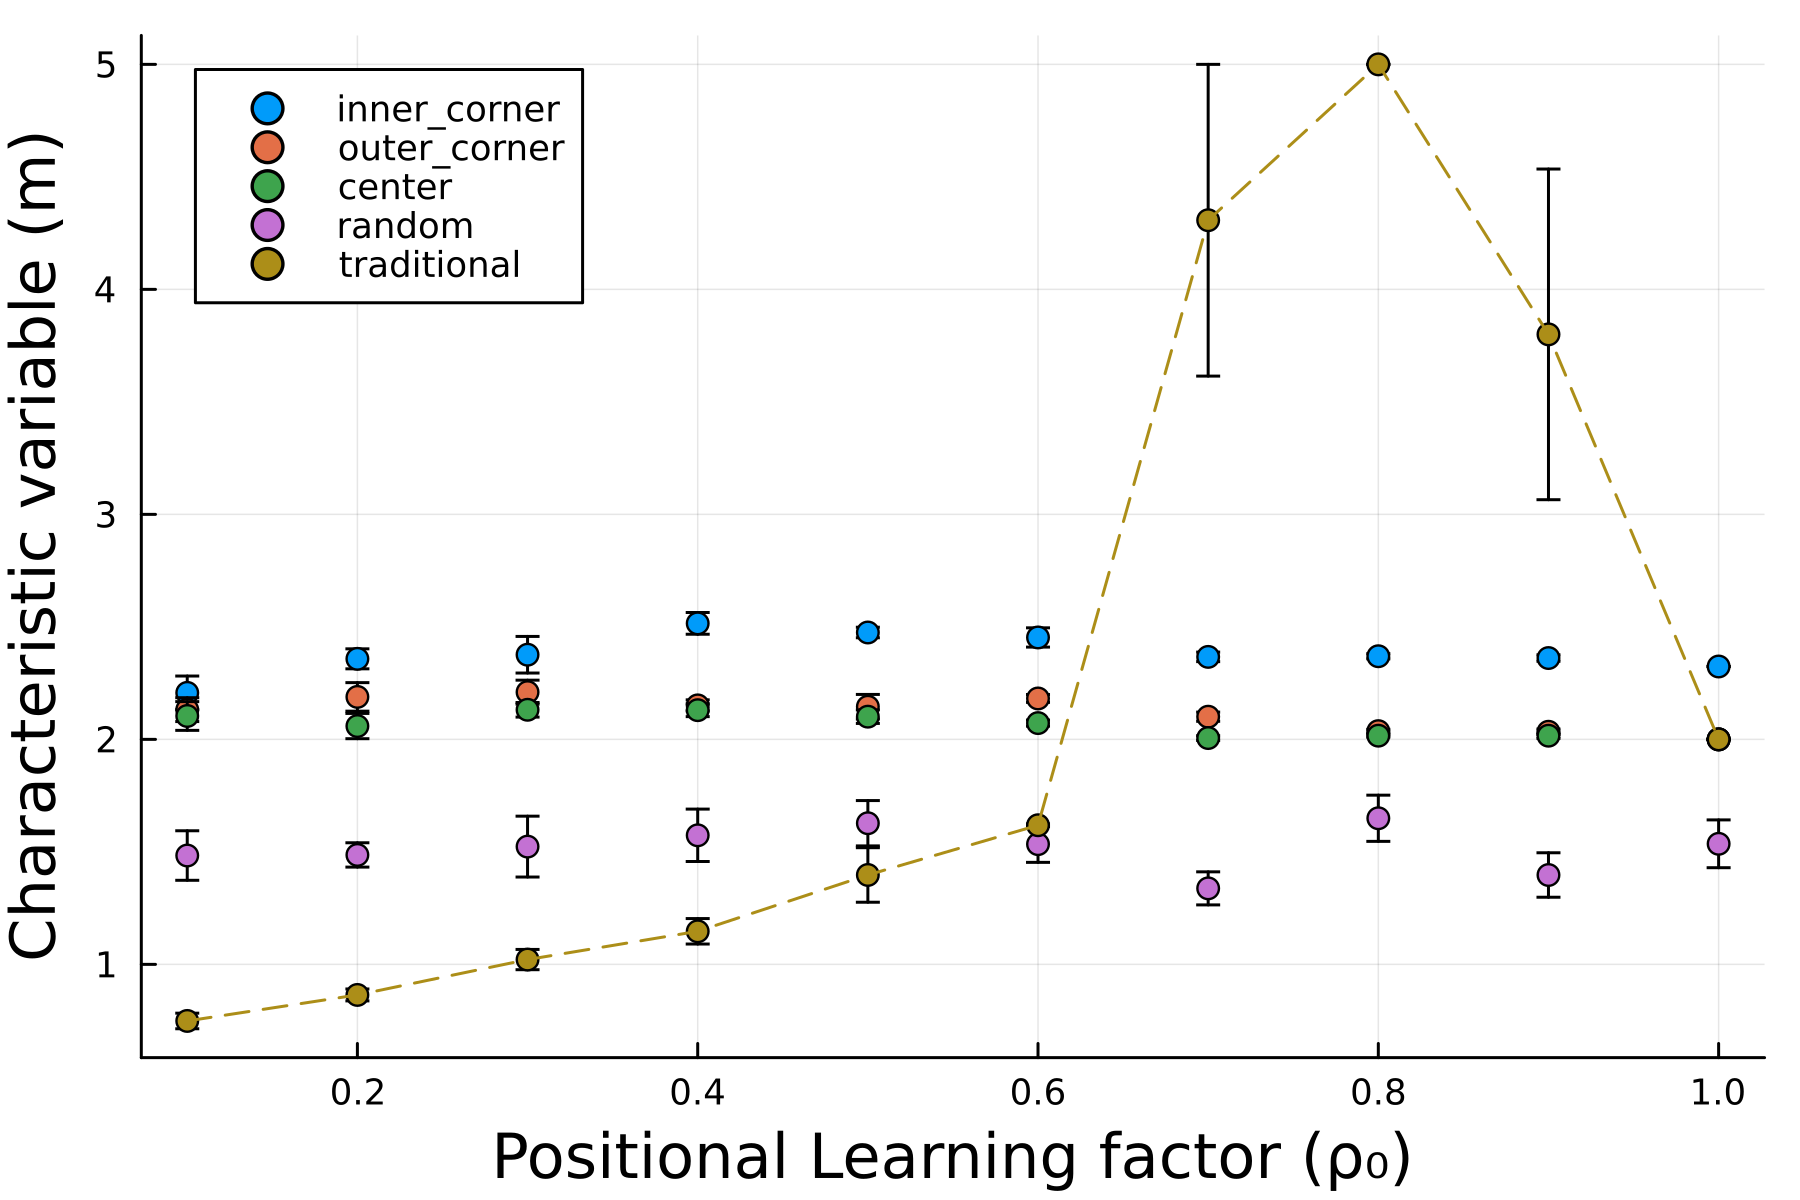
\includegraphics[width=0.45\textwidth]{figures/2D-BPCA-analysis/m-32.png}}
    \subfigure[$L=48$]{\label{fig:2DBPCA m vs rho 48}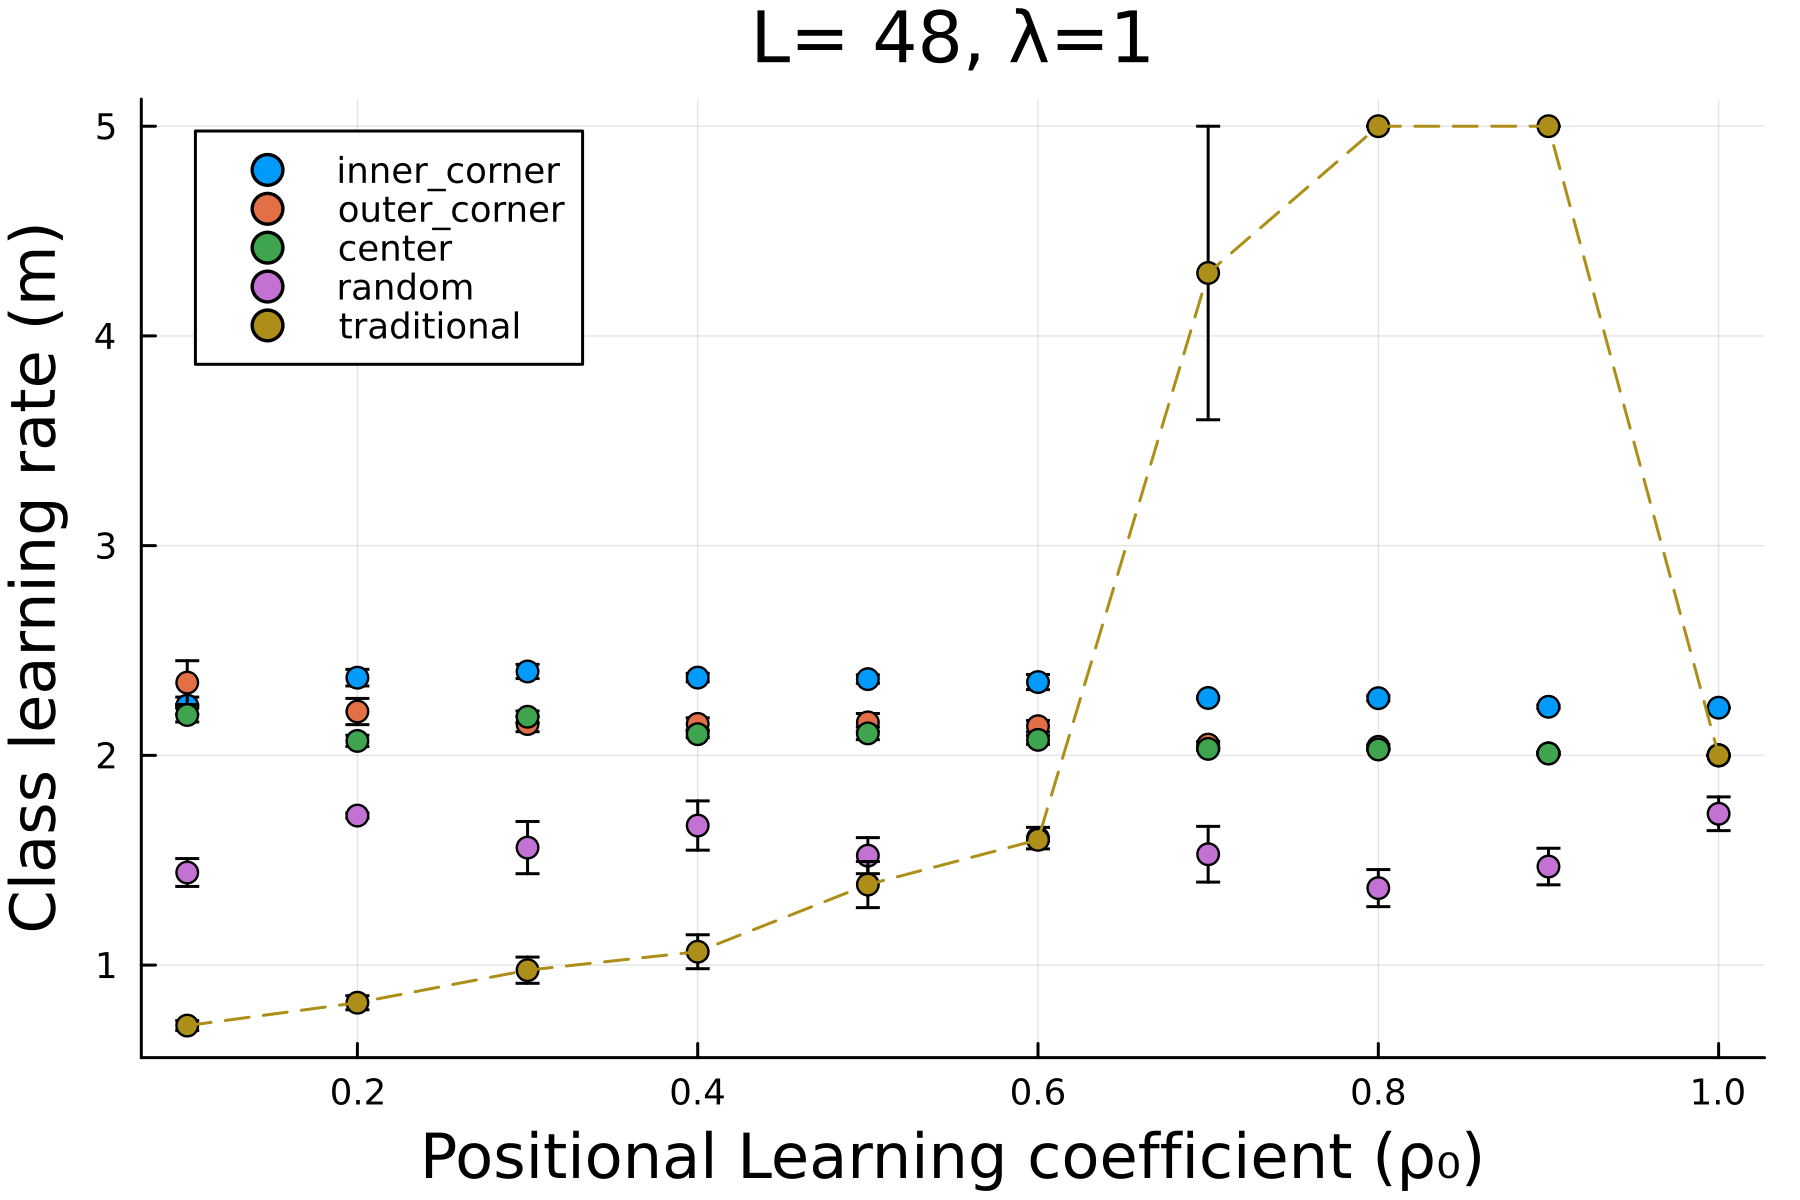
\includegraphics[width=0.45\textwidth]{figures/2D-BPCA-analysis/m-48.png}}
    \subfigure[$L=64$]{\label{fig:2DBPCA m vs rho 64}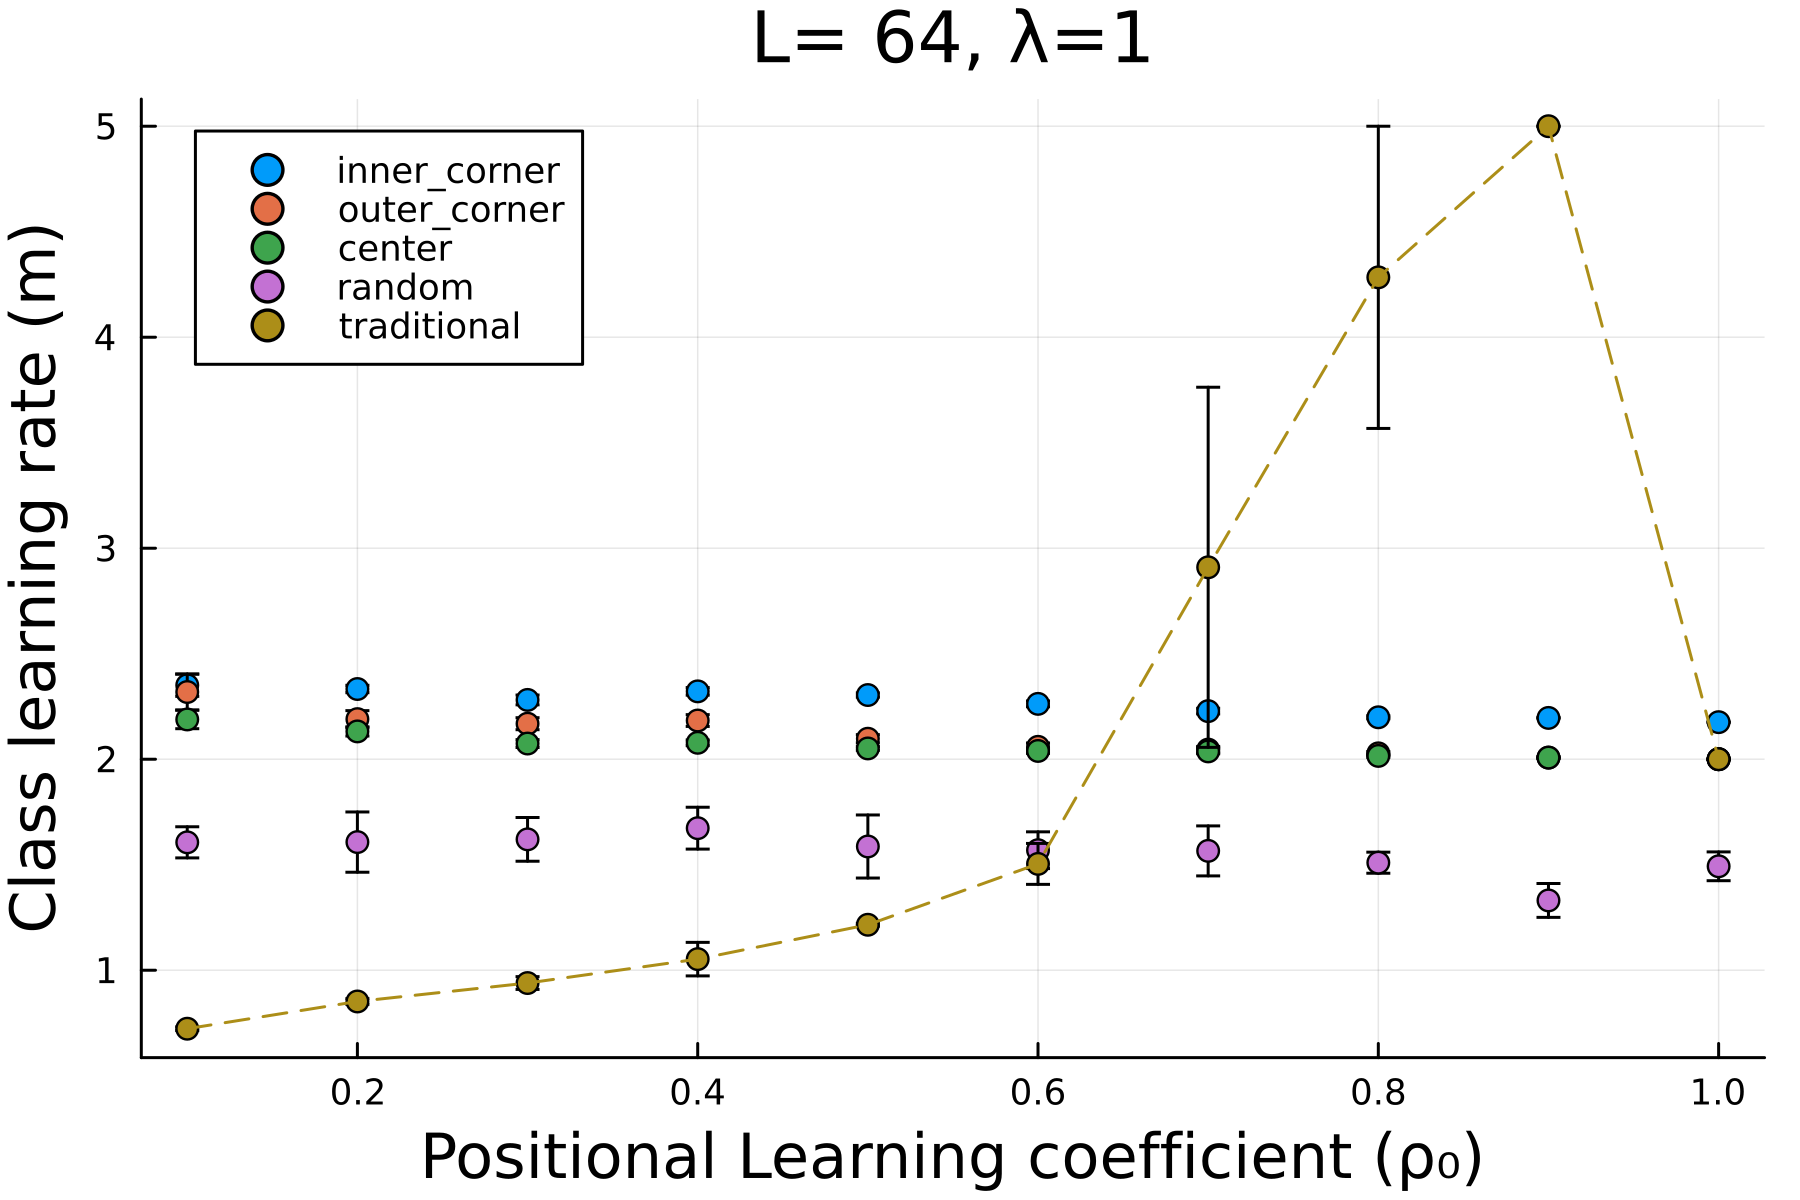
\includegraphics[width=0.45\textwidth]{figures/2D-BPCA-analysis/m-64.png}}
    \subfigure[$L=96$]{\label{fig:2DBPCA m vs rho 96}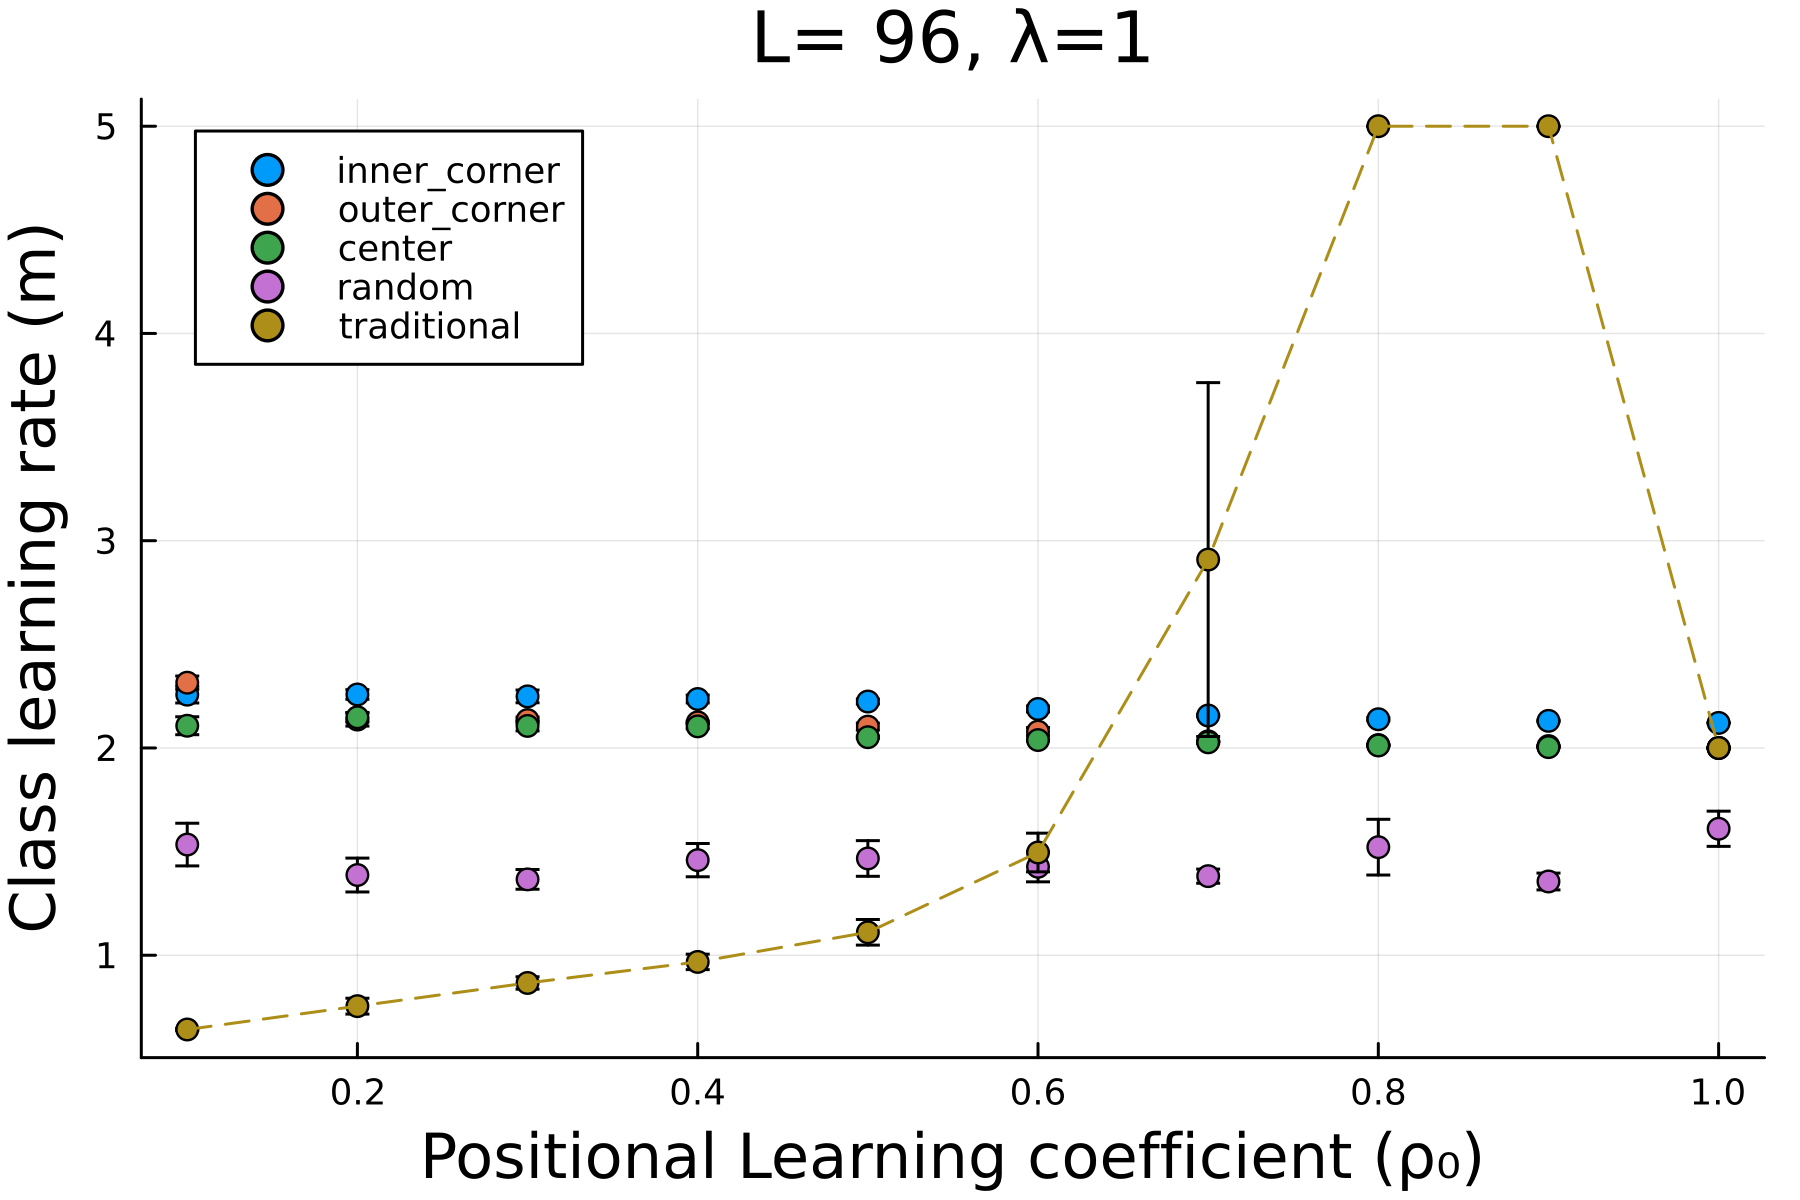
\includegraphics[width=0.45\textwidth]{figures/2D-BPCA-analysis/m-96.png}}
    \subfigure[$L=128$]{\label{fig:2DBPCA m vs rho 128}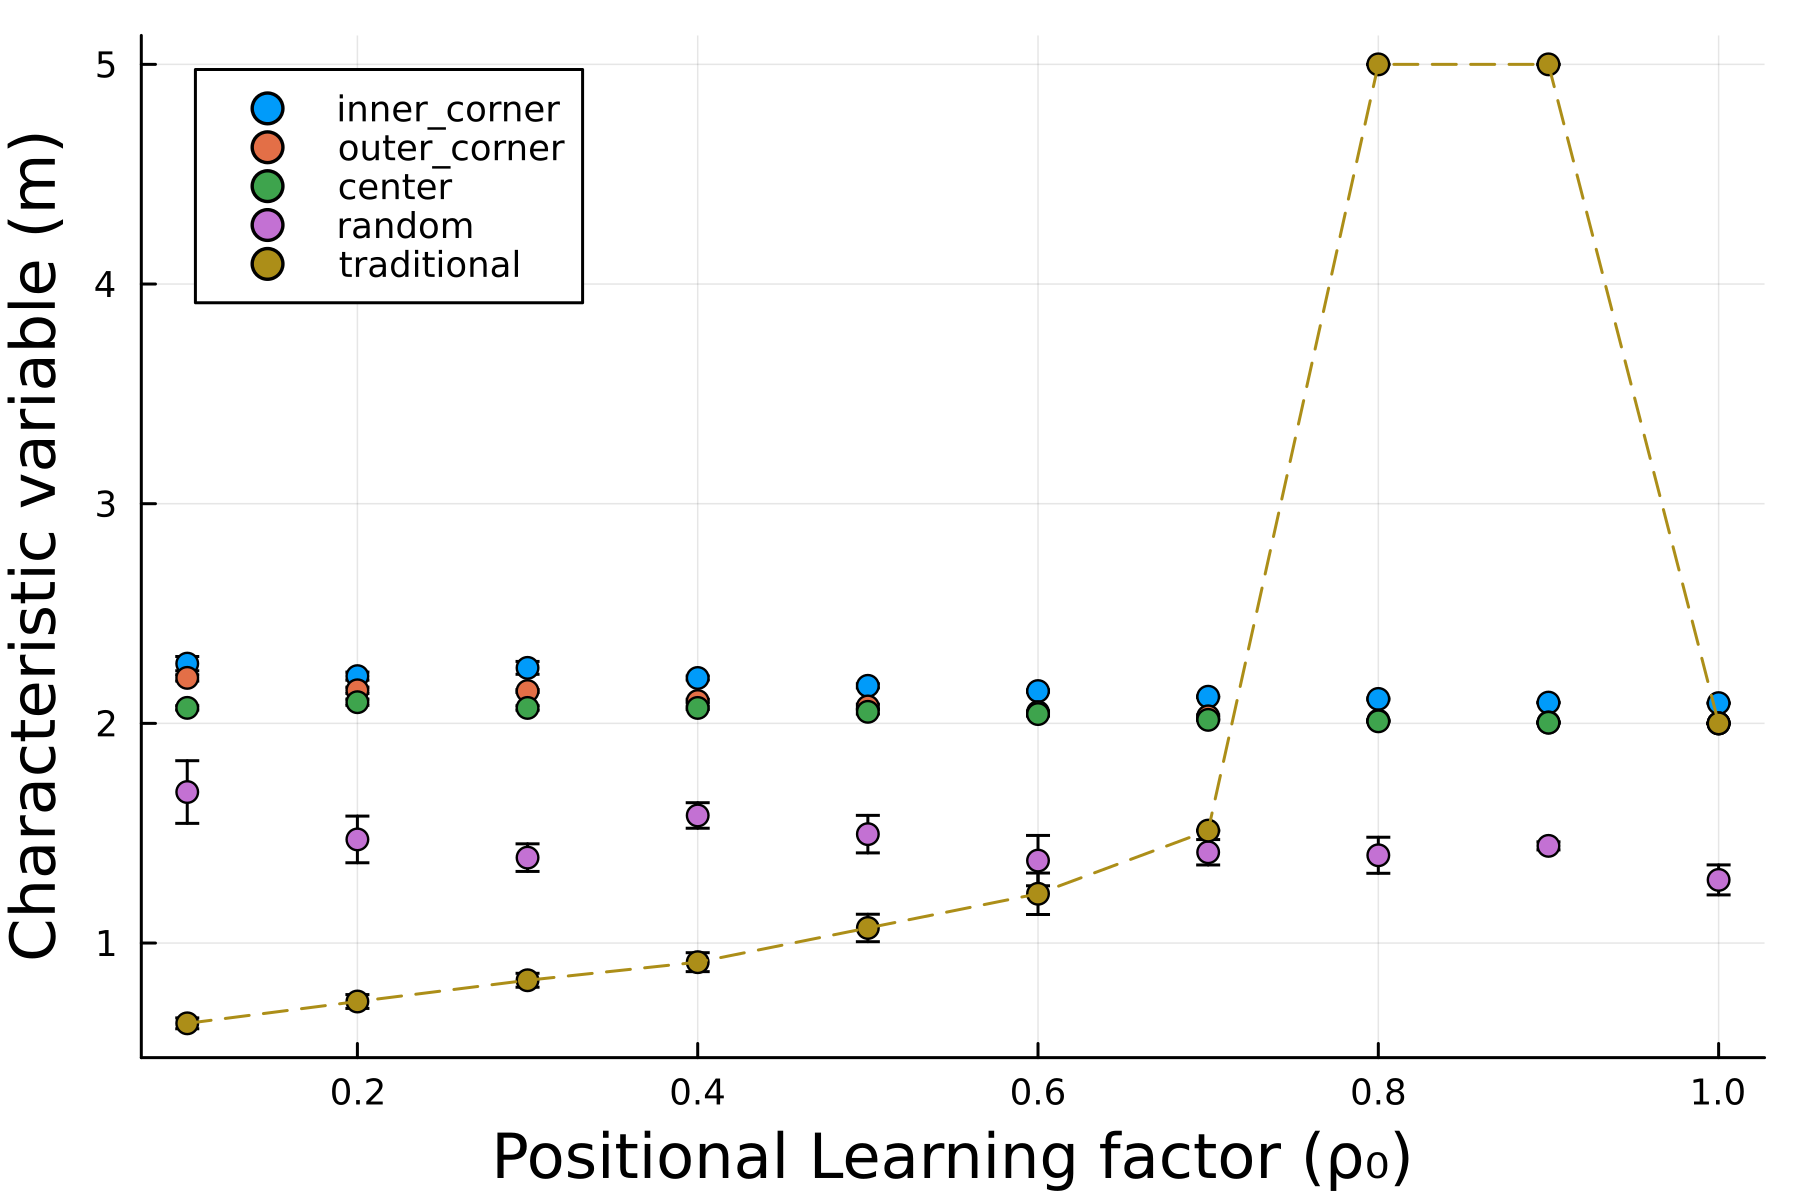
\includegraphics[width=0.45\textwidth]{figures/2D-BPCA-analysis/m-128.png}}
    \caption{Learning rate $m$ as a function of positional learning factor $\rho_0$ for different classroom sizes $L \in \lbrace 32,48,64,96,128 \rbrace$. Higher learning rate $m$ values indicate better performance.}
    \label{fig:2DBPCA m vs rho}
\end{figure}

\newpage

\subsection{Time to learn $t_{max}$ vs class size $N$} \label{subsec: 2DBPCA tmax vs N}
\begin{figure}[h!]
    \centering
    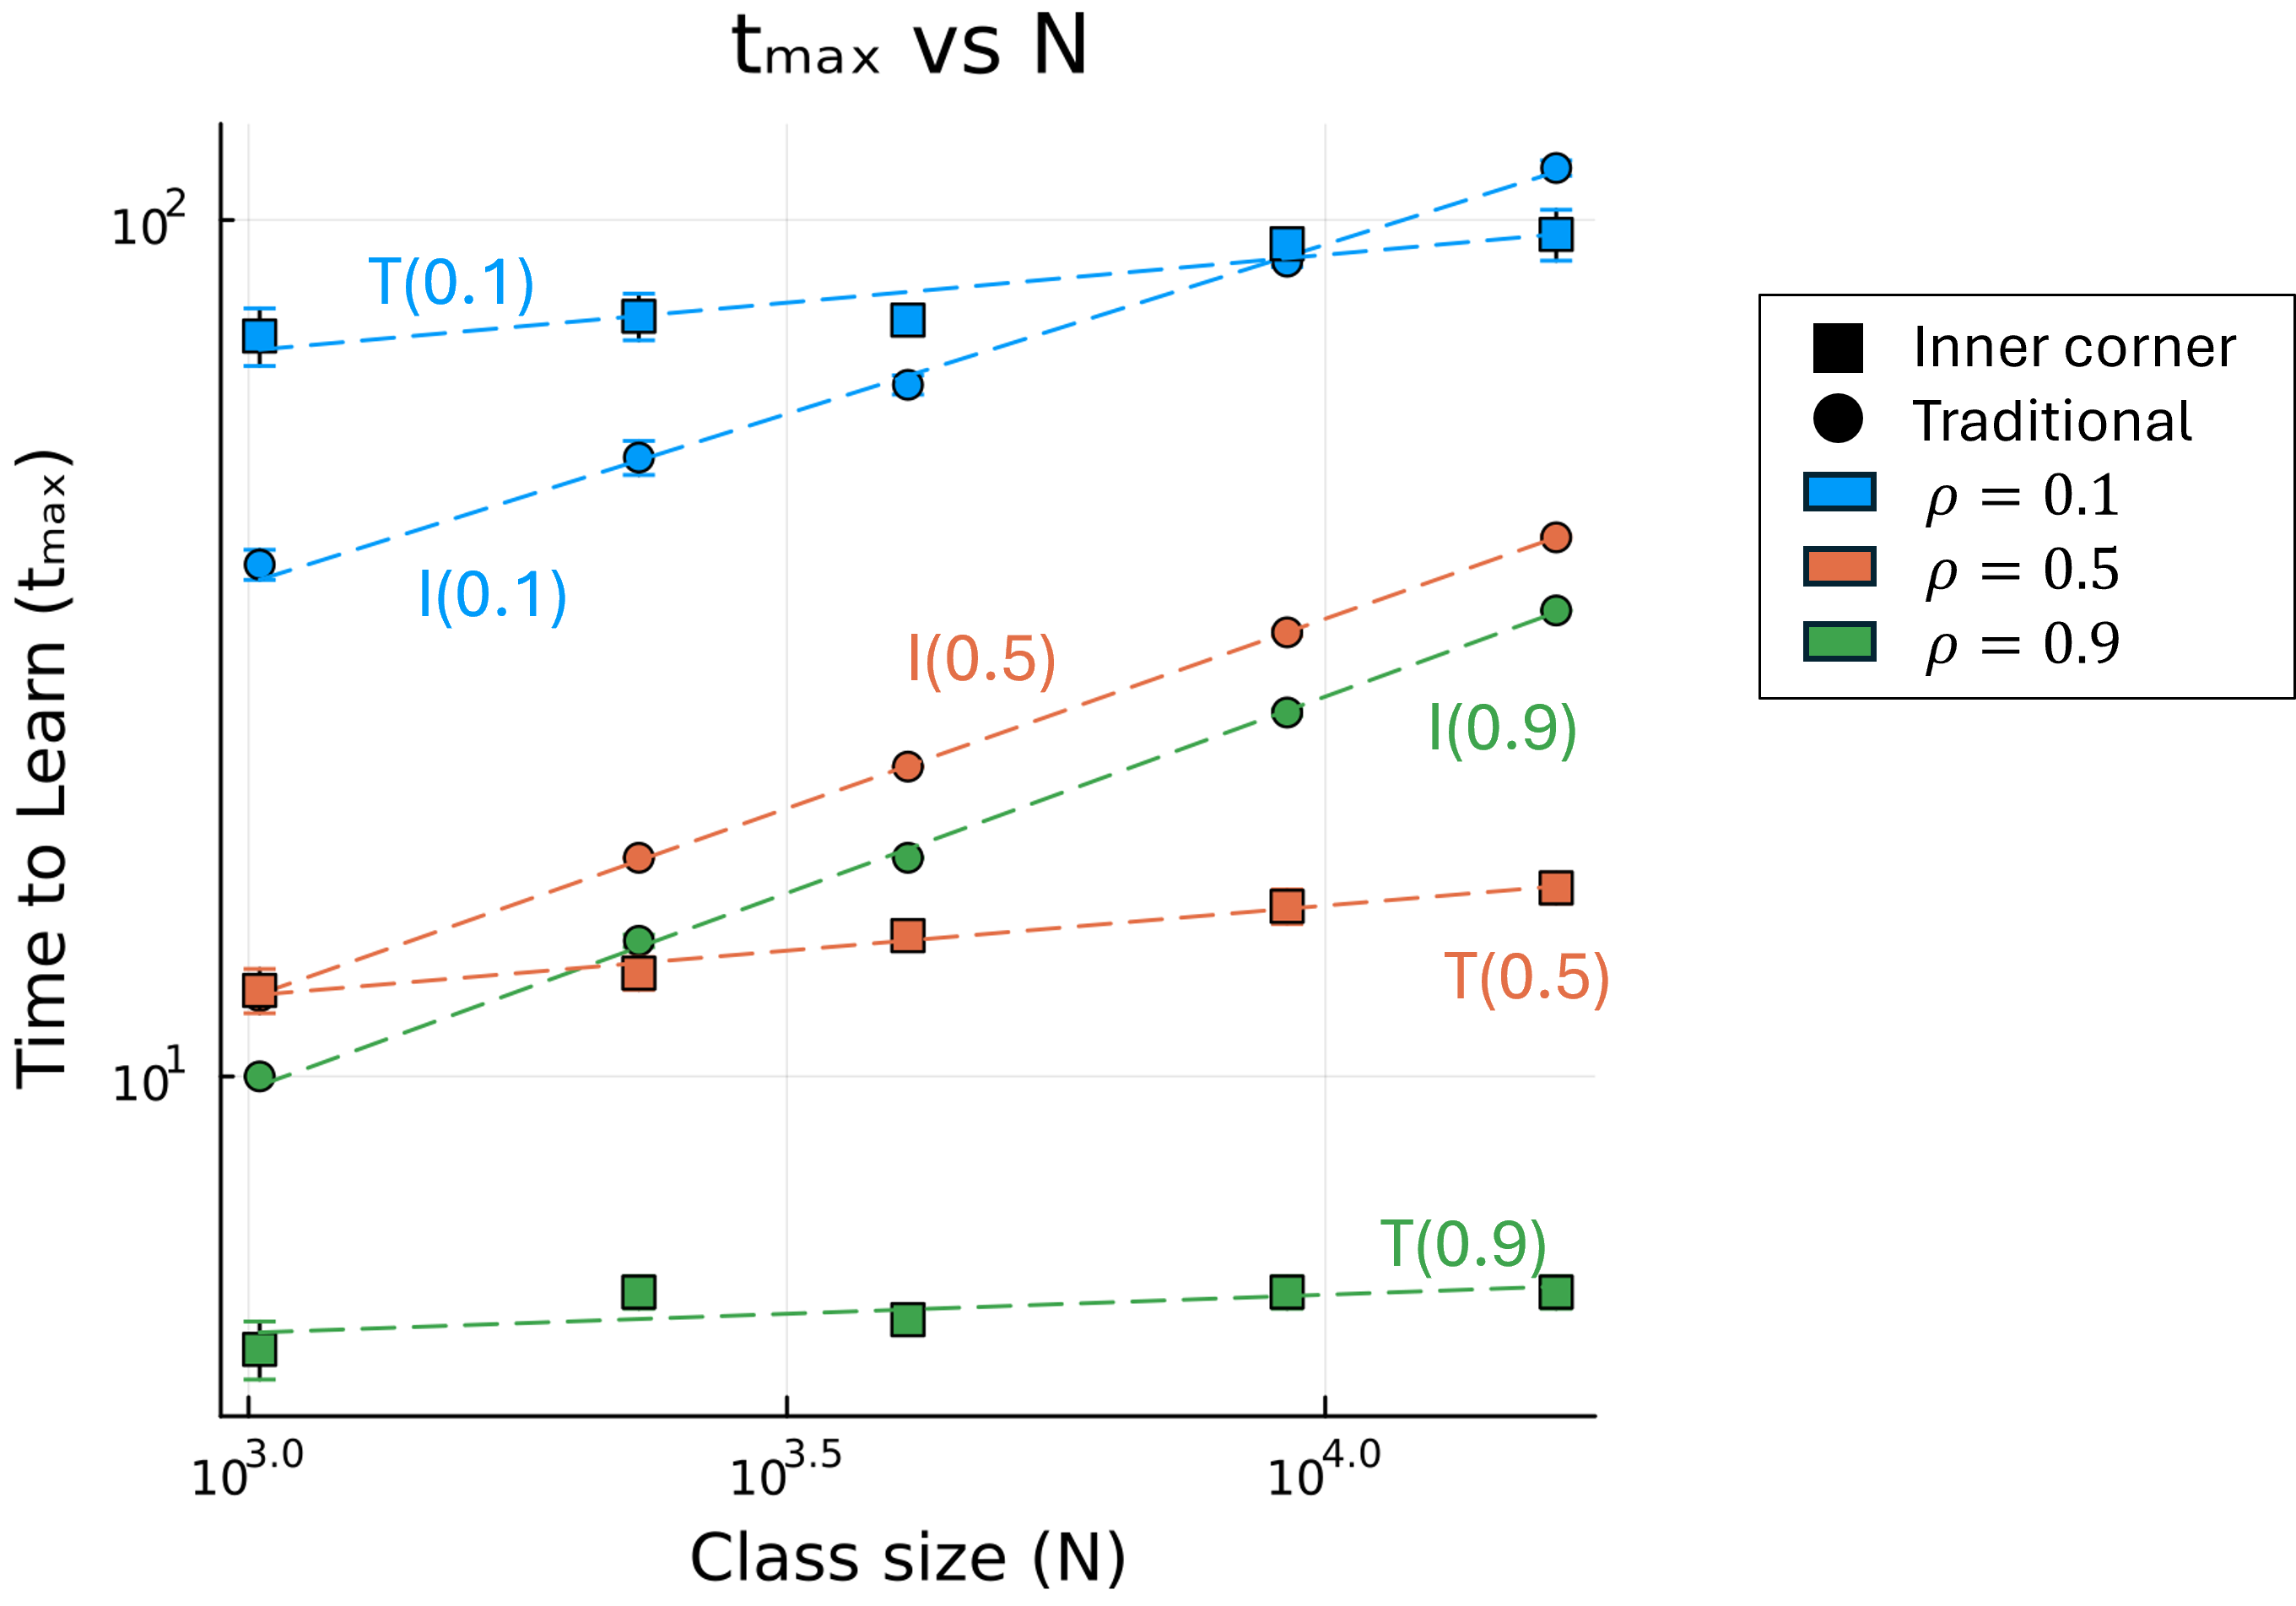
\includegraphics[width=0.8\textwidth]{figures/2D-BPCA-analysis/N_vs_tmax-traditional-inner_corner.png}
    \caption[Class size dependence of time to learn in homogenous models]{Maximum time $t_{max}$ as a function of class size $N$ for P2P and traditional models. Circles and squares denote data points for the inner corner P2P configuration and traditional learning model, respectively. The dash lines are the corresponding power law fit of the form $t_{max}=a \cdot N^b$ using $\rho \in \lbrace 0.1, 0.5, 0.9 \rbrace$. The fitted parameters are shown in the table with an average of $\langle b \rangle = 0.4532 \pm 0.019$ for the inner corner and $\langle b \rangle = 0.087\pm0.021$ for the traditional model.}
    \label{fig:Traditional vs PI tmax vs N}
\end{figure}

\begin{table}[htbp!]
  \centering
  
  \begin{tabular}{|c|cc|cc|}
    \hline
    & \multicolumn{2}{c|}{\textbf{Inner corner}}       & \multicolumn{2}{c|}{\textbf{Traditional}}        \\ \cline{2-5} 
    & \multicolumn{1}{c|}{\textbf{$a$}} & \textbf{$b$} & \multicolumn{1}{c|}{\textbf{$a$}} & \textbf{$b$} \\ \hline
    \textbf{$\lambda=0.1$} & \multicolumn{1}{c|}{2.4515}       & 0.3955       & \multicolumn{1}{c|}{32.4884}      & 0.1119       \\ \hline
    \textbf{$\lambda=0.5$} & \multicolumn{1}{c|}{0.5795}       & 0.4428       & \multicolumn{1}{c|}{6.0079}       & 0.1052       \\ \hline
    \textbf{$\lambda=0.9$} & \multicolumn{1}{c|}{0.4055}       & 0.4589       & \multicolumn{1}{c|}{3.6914}       & 0.0445       \\ \hline
  \end{tabular}
  \caption{Power law fit parameters $a$ and $b$ for $t_{max}$ vs $N$, where $t_{max}=a \cdot N ^ b$}
  \label{tab:2DBPCA tmax vs N fit params}
\end{table}

When we analyze the dependence of the time to learn $t_{max}$ on the class size $N$, we find that the trend for both models follow the power law $t_{max} = a \cdot N^b$. In Figure \ref{fig:Traditional vs PI tmax vs N} we observe break-even points where the traditional model becomes more efficient than the PI model. These points happen at lower class sizes and lower $\rho$ values. We also find two major groups of power laws based on their $b$ values, as summarized in Table \ref{tab:2DBPCA tmax vs N fit params}. The first group has an average $b$ value of $\langle b \rangle = 0.4532 \pm 0.019$ for the inner corner configuration, while the second group has an average $b$ value of $\langle b \rangle = 0.087\pm0.021$ for the traditional model. The inner corner configuration has higher $b$ values than the traditional model, indicating that the traditional model is less affected by class size $N$ and so is more scalable than the PI model.

\section{Discussion/conclusions?}
In this chapter, we have shown that between different seating arrangements for the PI model, the inner corner SA is the most efficient in terms of time to learn $t_{max}$ and learning rate $m$. The outer corner and center SAs performed similarly worse than the inner corner SA, while the random configuration performed the worst. This is different from what existing literature has shown, where the outer corner SA is the most efficient \cite{roxas2010seating}. This is likely because of the simplifications made in our model. Our model does not incorporate factors such as the similarity effect mentioned in previous studies \cite{roxas2010seating,smith2009peer}. This effect is the phenomenon where in students of similar aptitude levels tend to learn better when seated together and are able to learn from each other regardless their actual aptitude. Our model also does not consider anisotropic positional learning factors $\rho_{i,j}$, where the probability of learning from a neighbor varies with the neighbors' relative positions. Besides being binary, which introduces granularity, our model also does not consider that not all students are equally receptive to peer instruction or have the same learning rate. Introducing these factors, which we will explore in the next chapters, may make our model reflect reality better and provide us with better understanding of the learning dynamics in the classroom.

The nature of our model lends itself to be heavily influenced by geometric factors. The most impactful factor in this case is then the distance $d_{max}$ of any student to a high aptitude or learned student as shown in figure \ref{fig:SA dmax}. The inner corner SA minimizes $d_{max}$, which is why it is the most efficient. The outer corner and center SAs have equal $d_{max}$ higher than the inner corner SA, which explains why they performed very similarly albeit worse than the inner corner SA.

\begin{figure}[htbp!]
    \centering
    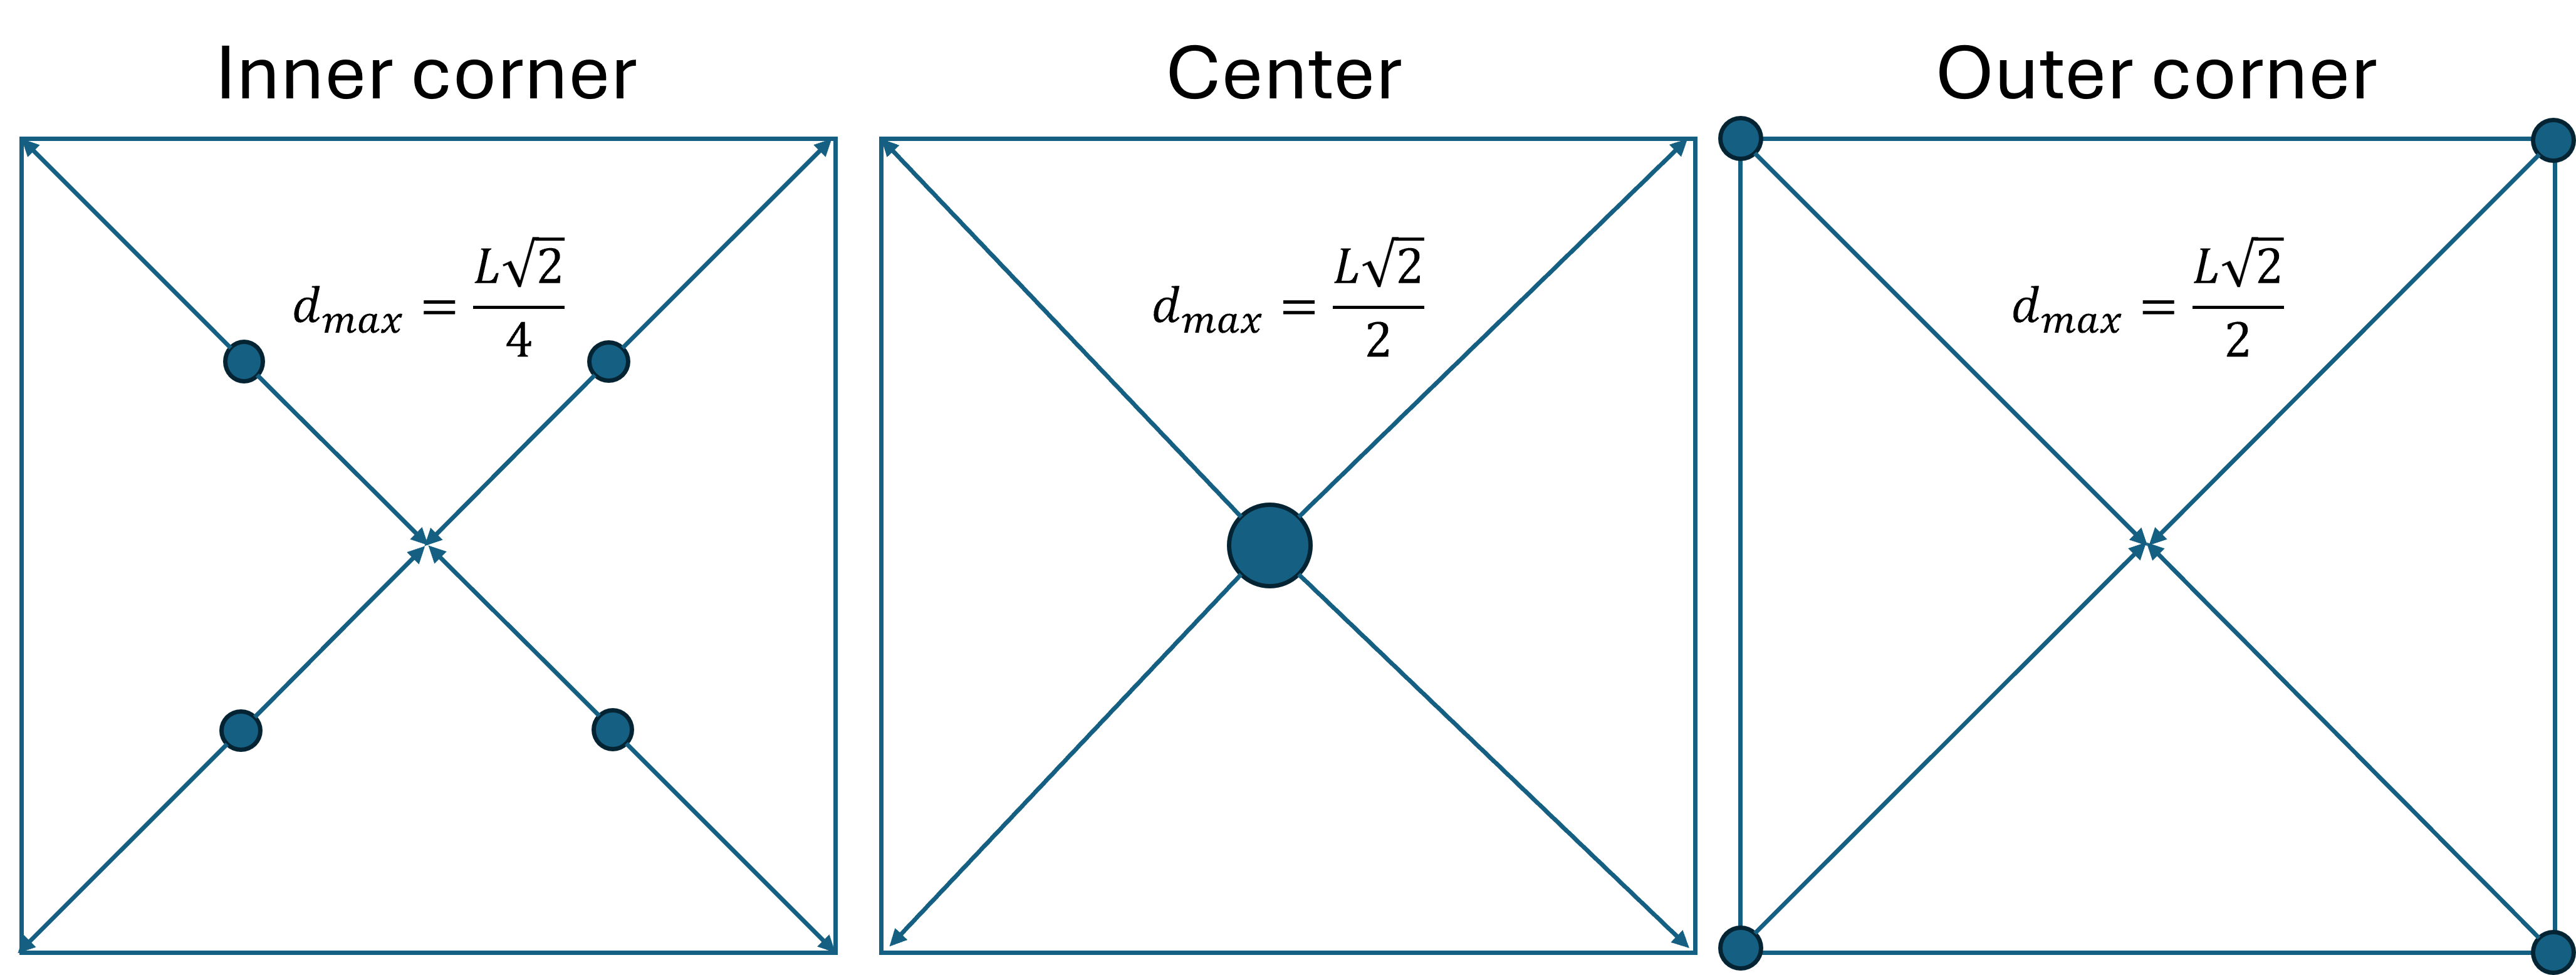
\includegraphics[width=0.8\textwidth]{figures/SA dmax.png}
    \caption{Distance $d_{max}$ of any student to a high aptitude or learned student for different seating arrangements.}
    \label{fig:SA dmax}
\end{figure}

Our analysis on the dependence of $t_{max}$ on $N$ gives us an explanation on why the traditional model performed better than the PI model in most cases. With lower $b$-values, the traditional model is less affected by class size than the PI models are. Because of this, the traditional model performed better in cases with larger classrooms. 

With regards to the performance of PI methods with traditional teaching methods, we found that classrooms with higher $\rho_0$ values performed better in PI models, while classrooms with lower $\rho_0$ values performed better in traditional models. A previous similar study \cite{roxas2010seating} found that classes with lower aptitude levels were the ones who benefited the most from the PI methods. Although we cannot directly conclude this from our model, we were able to show that students with a lower probability of learning or students who learn slower, can benefit as much from PI as in traditional set ups. This reinforces other studies' findings \cite{lasry2008peer} that show that PI methods can be effective even regardless of the students' actual aptitude levels.

    

% !TEX root =  main.tex
\chapter{Heterogeneous Learning Rates}

To introduce learning rate heterogeneity in the classroom, we revisit equation \ref{eq:BPCA PI learning probability}. 
\begin{equation*}
    P_{ij} = 1 - \prod_{\forall \delta i, \delta j}{\lbrack1-(\lambda_{ij})(\rho_{i+\delta i, j+\delta j})(s_{i+\delta i, j+\delta j})}\rbrack
    \tag{\ref{eq:BPCA PI learning probability} revisted}
\end{equation*}
We can adjust the parameter $\lambda_{ij}$ to introduce differences in each student's learning rate. 
We set a student's learning rate as $\lambda_{ij} = \lambda_0 \pm \delta\lambda$ where $\delta\lambda \in \lbrace 0.0,0.1, 0.2, 0.3, 0.4\rbrace$ and $\lambda_0 = 0.5$. 
Each student has an equal chance of having a learning rate that is either faster $(\lambda_0 + \delta\lambda)$ or slower $(\lambda_0 - \delta\lambda)$ than the average learning rate $\lambda_0$. 

$\lambda_{i,j} \in [0,1]$ is the learning rate of student $c_{i,j}$ with values $\lambda_{i,j} = \lbrace \lambda_0 \pm \delta \lambda \rbrace$ where $\lambda_0 = 0.5$ and $\delta \lambda = \lbrace 0.1, 0.2, 0.3, 0.4 \rbrace$, 

\section{Effects on classroom evolution}\label{sec:BPCAIH effects on classroom evolution}
\subsection{Peer Instruction (PI)}\label{sec:BPCAIH effects on classroom evolution PI}
When introducing heterogeneity to PI set ups, we see that the general trend of the classroom evolution is still the same as the homogenous case.
As shown in the figures in this section, we notice values of $\rho_0$ is still the most important factor in determining class performance. 
However, irregularities in the shapes of the ``wave of learning" become more pronounced for lower values of $\rho_0$ and high values of $\delta\lambda$ as shown in Figure~\ref{fig:2DBPCAIH sample class evolution low rho}.
These irregularities are also more pronounced at the start of the classroom and fades over time.
For high values of $\delta\lambda$, low values of $\rho_0$ leads to the irregularity in the ``wave of learning" to persist longer than those with higher values of $\rho_0$.
The irregularities in the shape of the ``wave of learning" and the deviation from the power law are less pronounced for higher values of $\rho_0$, regardless of the value of $\delta\lambda$, as shown in Figures \ref{fig:2DBPCAIH sample class evolution high rho} and \ref{fig:2DBPCAIH sample class evolution high rho high delta}.
In these cases, the class learning rate is slower than the power law fit at the start of the simulation.

\begin{figure}[htbp!]
   \centering
   \subfigure[$t=48$]{\label{fig:2DBPCAIH class evolution low rho 48}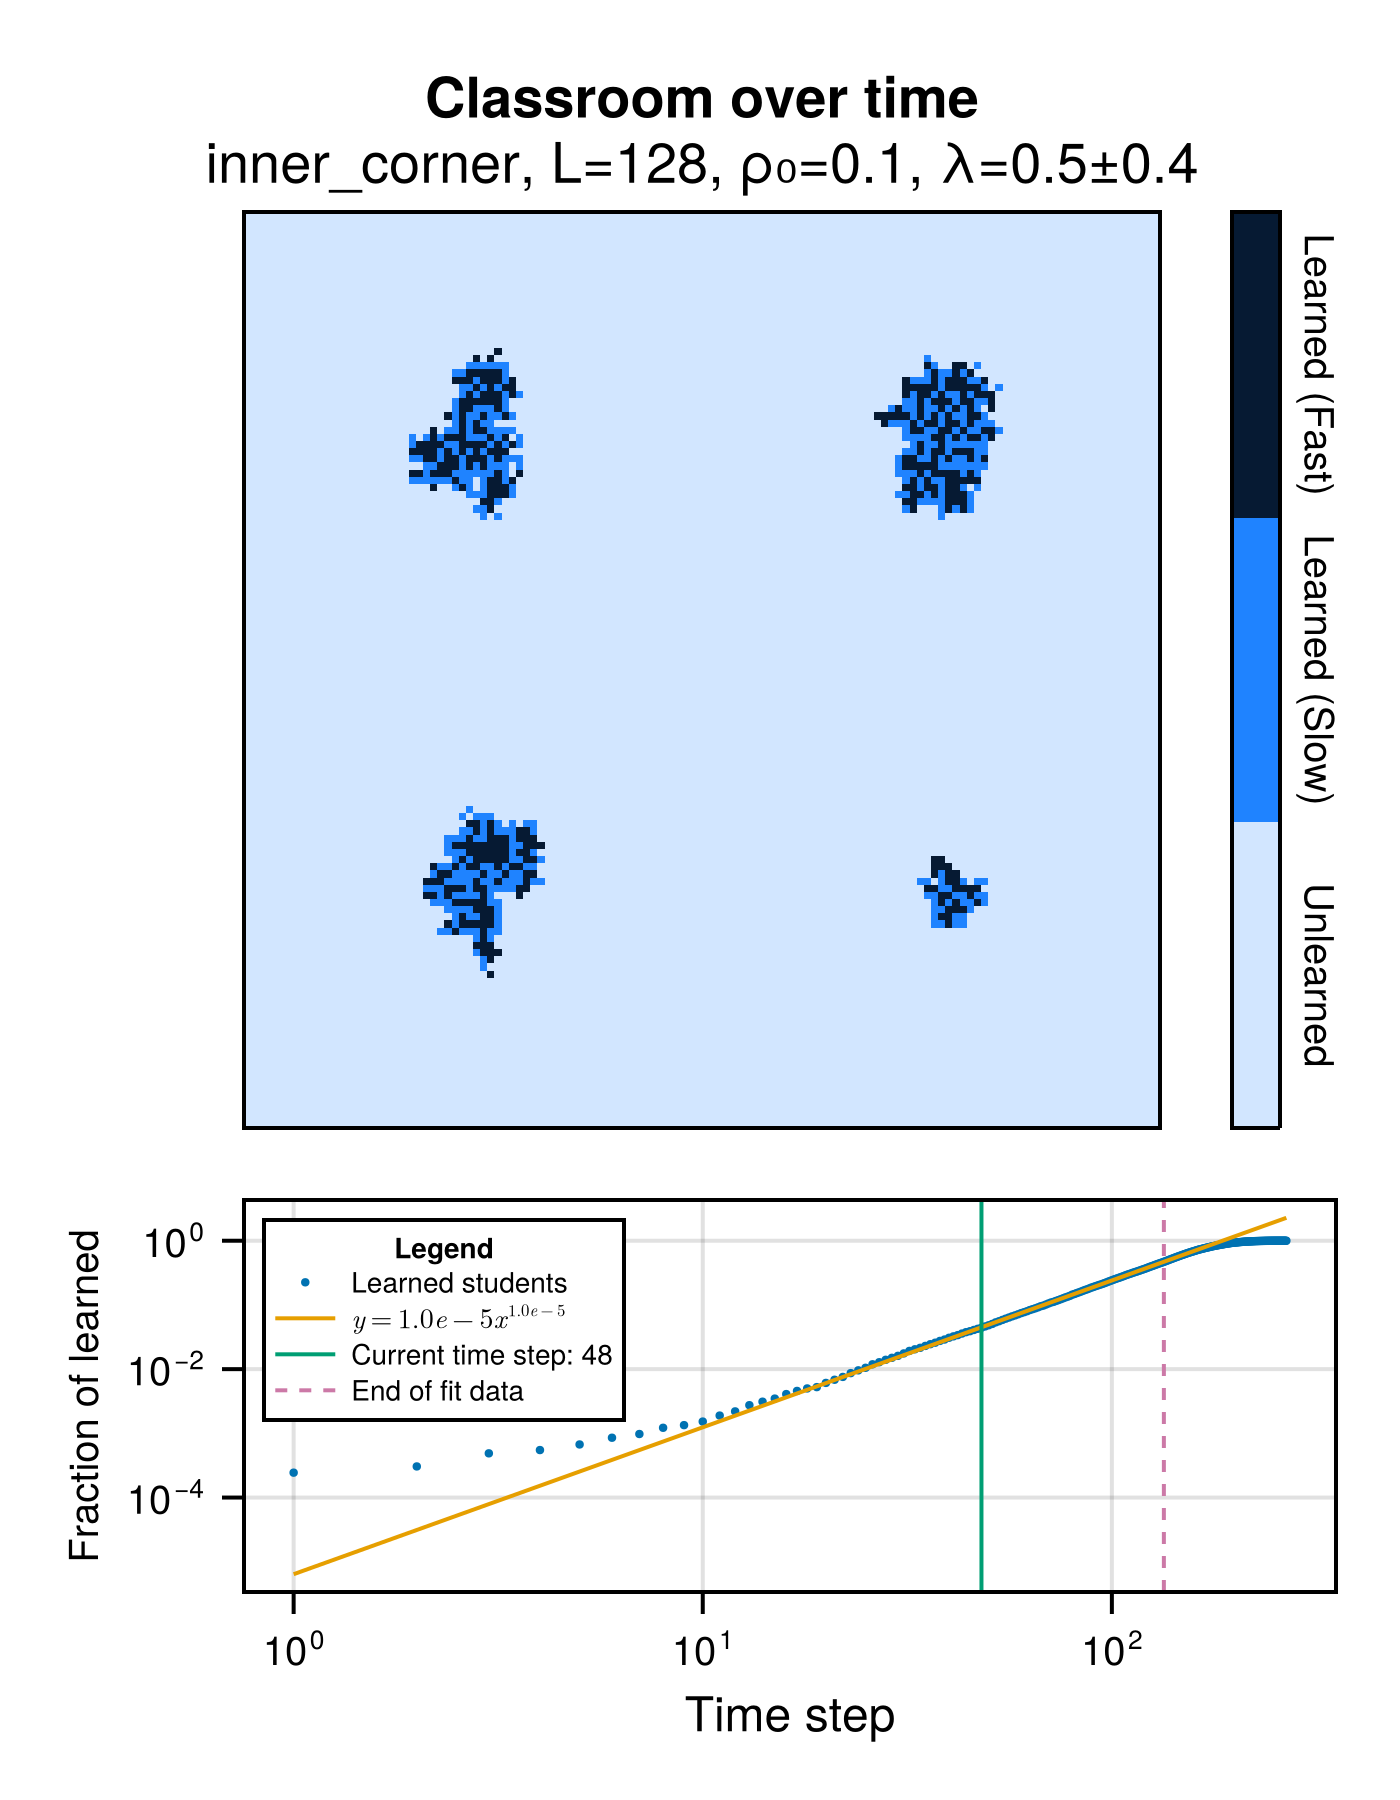
\includegraphics[width=0.40\textwidth]{figures/2D-BPCAIH-analysis/class evolutions/low rho/2DBPCAIH-inner_corner-128-0.1-0.5-0.4-trial_3-48.png}}
   \subfigure[$t=69$]{\label{fig:2DBPCAIH class evolution low rho 69}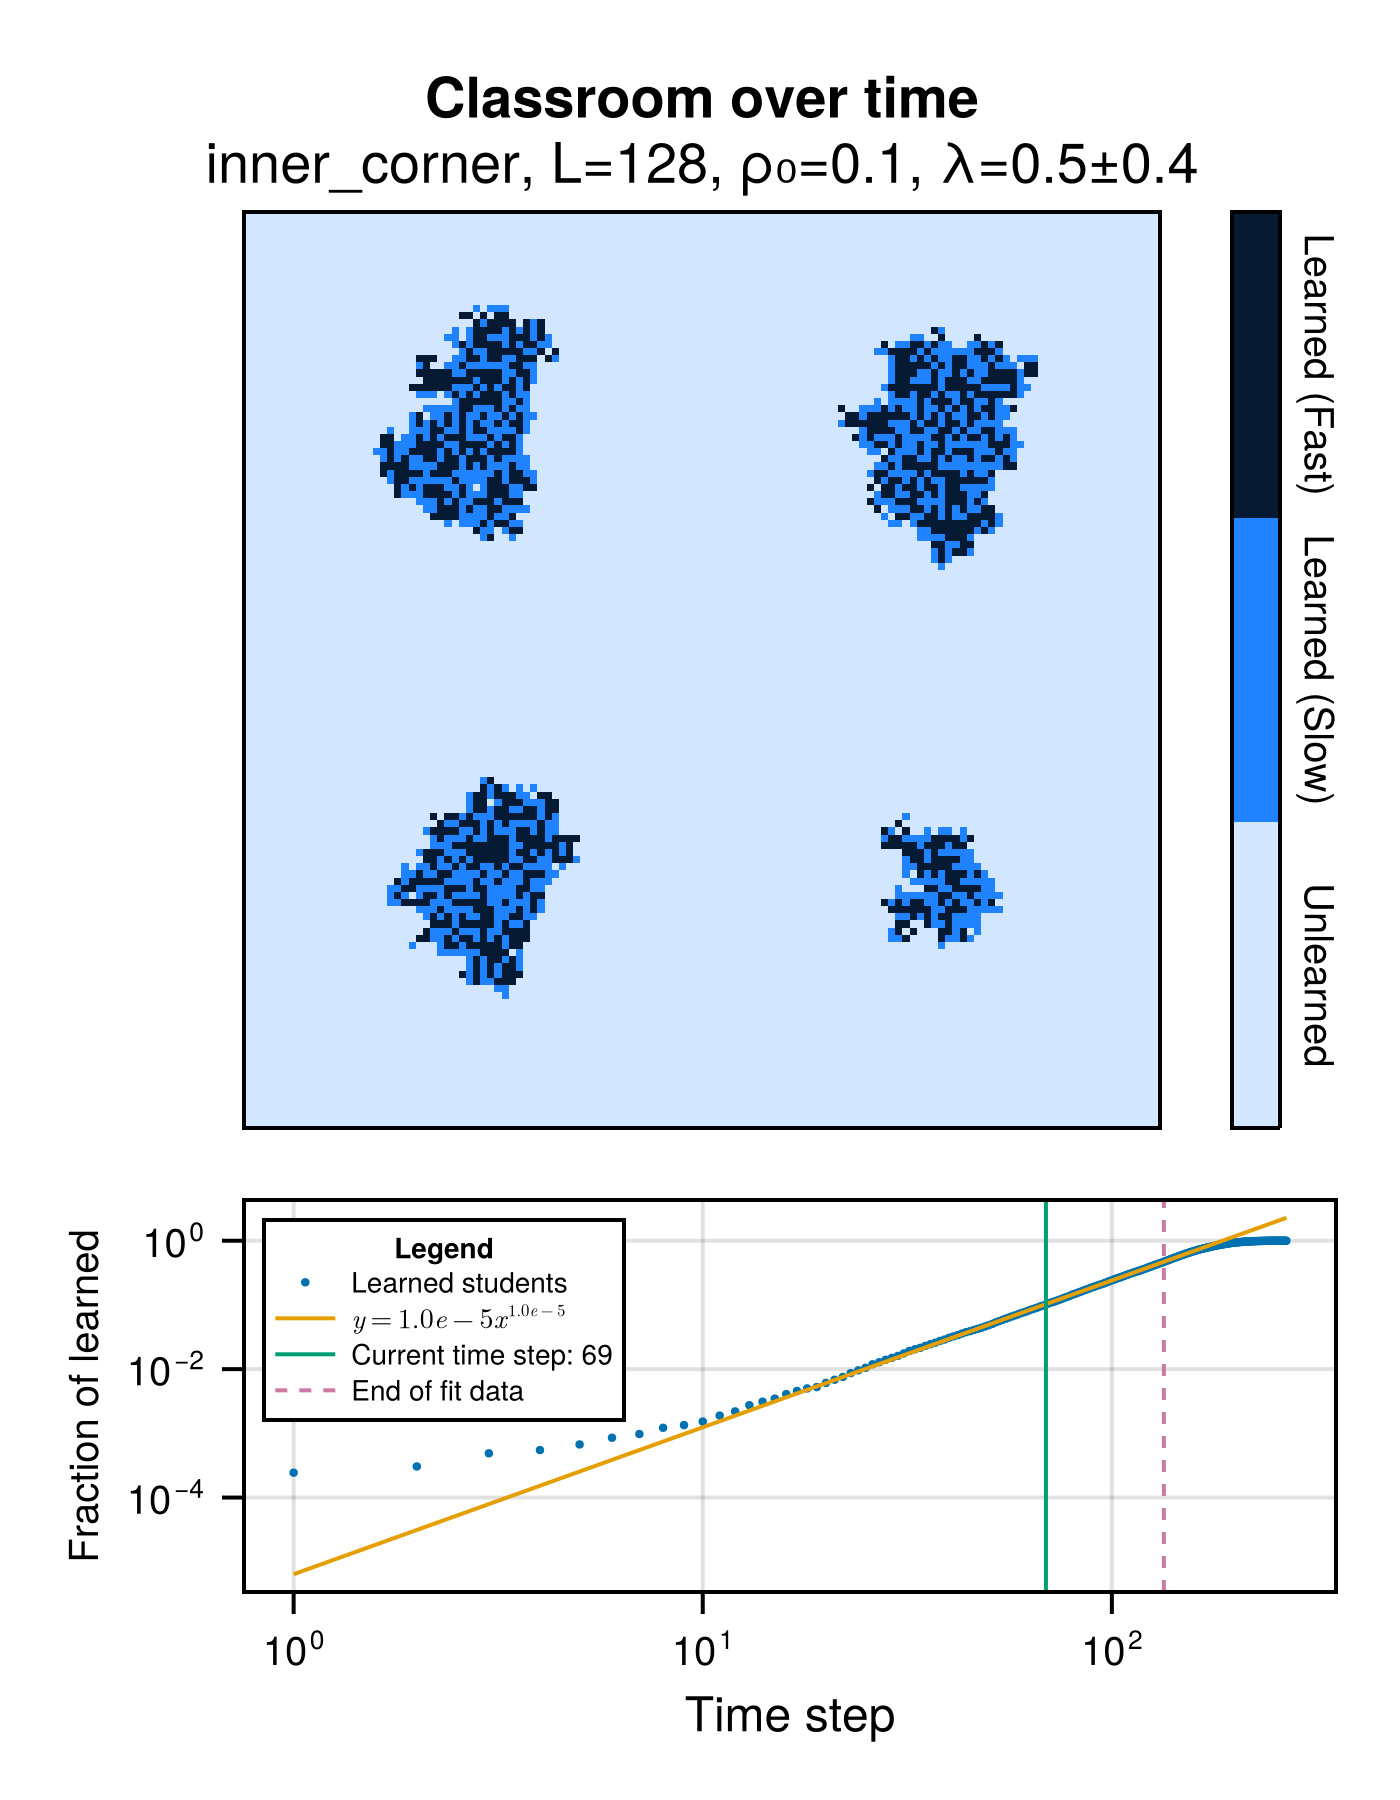
\includegraphics[width=0.40\textwidth]{figures/2D-BPCAIH-analysis/class evolutions/low rho/2DBPCAIH-inner_corner-128-0.1-0.5-0.4-trial_3-69.png}}
   \subfigure[$t=128$]{\label{fig:2DBPCAIH class evolution low rho 128}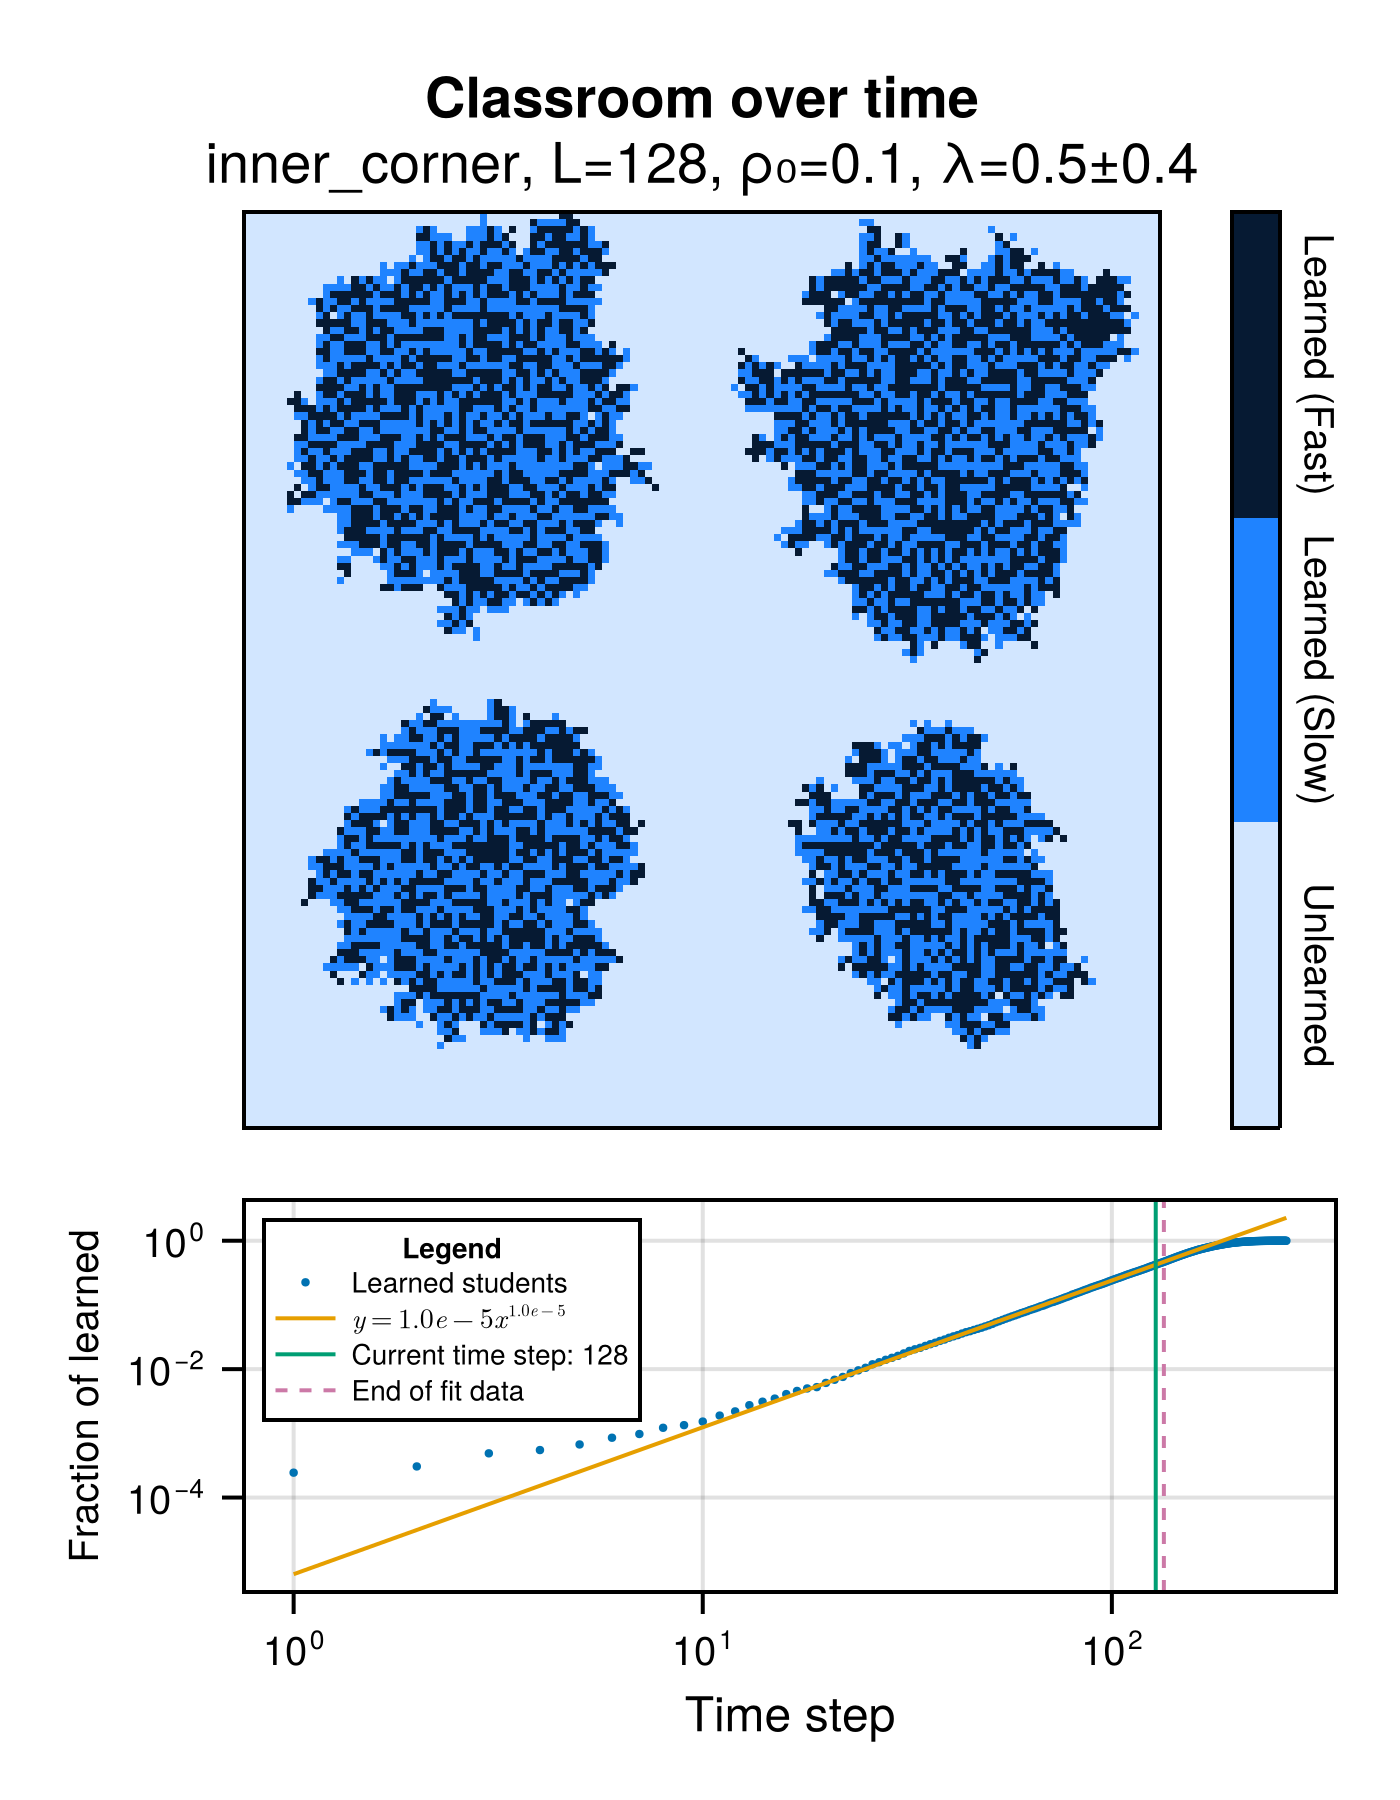
\includegraphics[width=0.40\textwidth]{figures/2D-BPCAIH-analysis/class evolutions/low rho/2DBPCAIH-inner_corner-128-0.1-0.5-0.4-trial_3-128.png}}
   \subfigure[$t=200$]{\label{fig:2DBPCAIH class evolution low rho 200}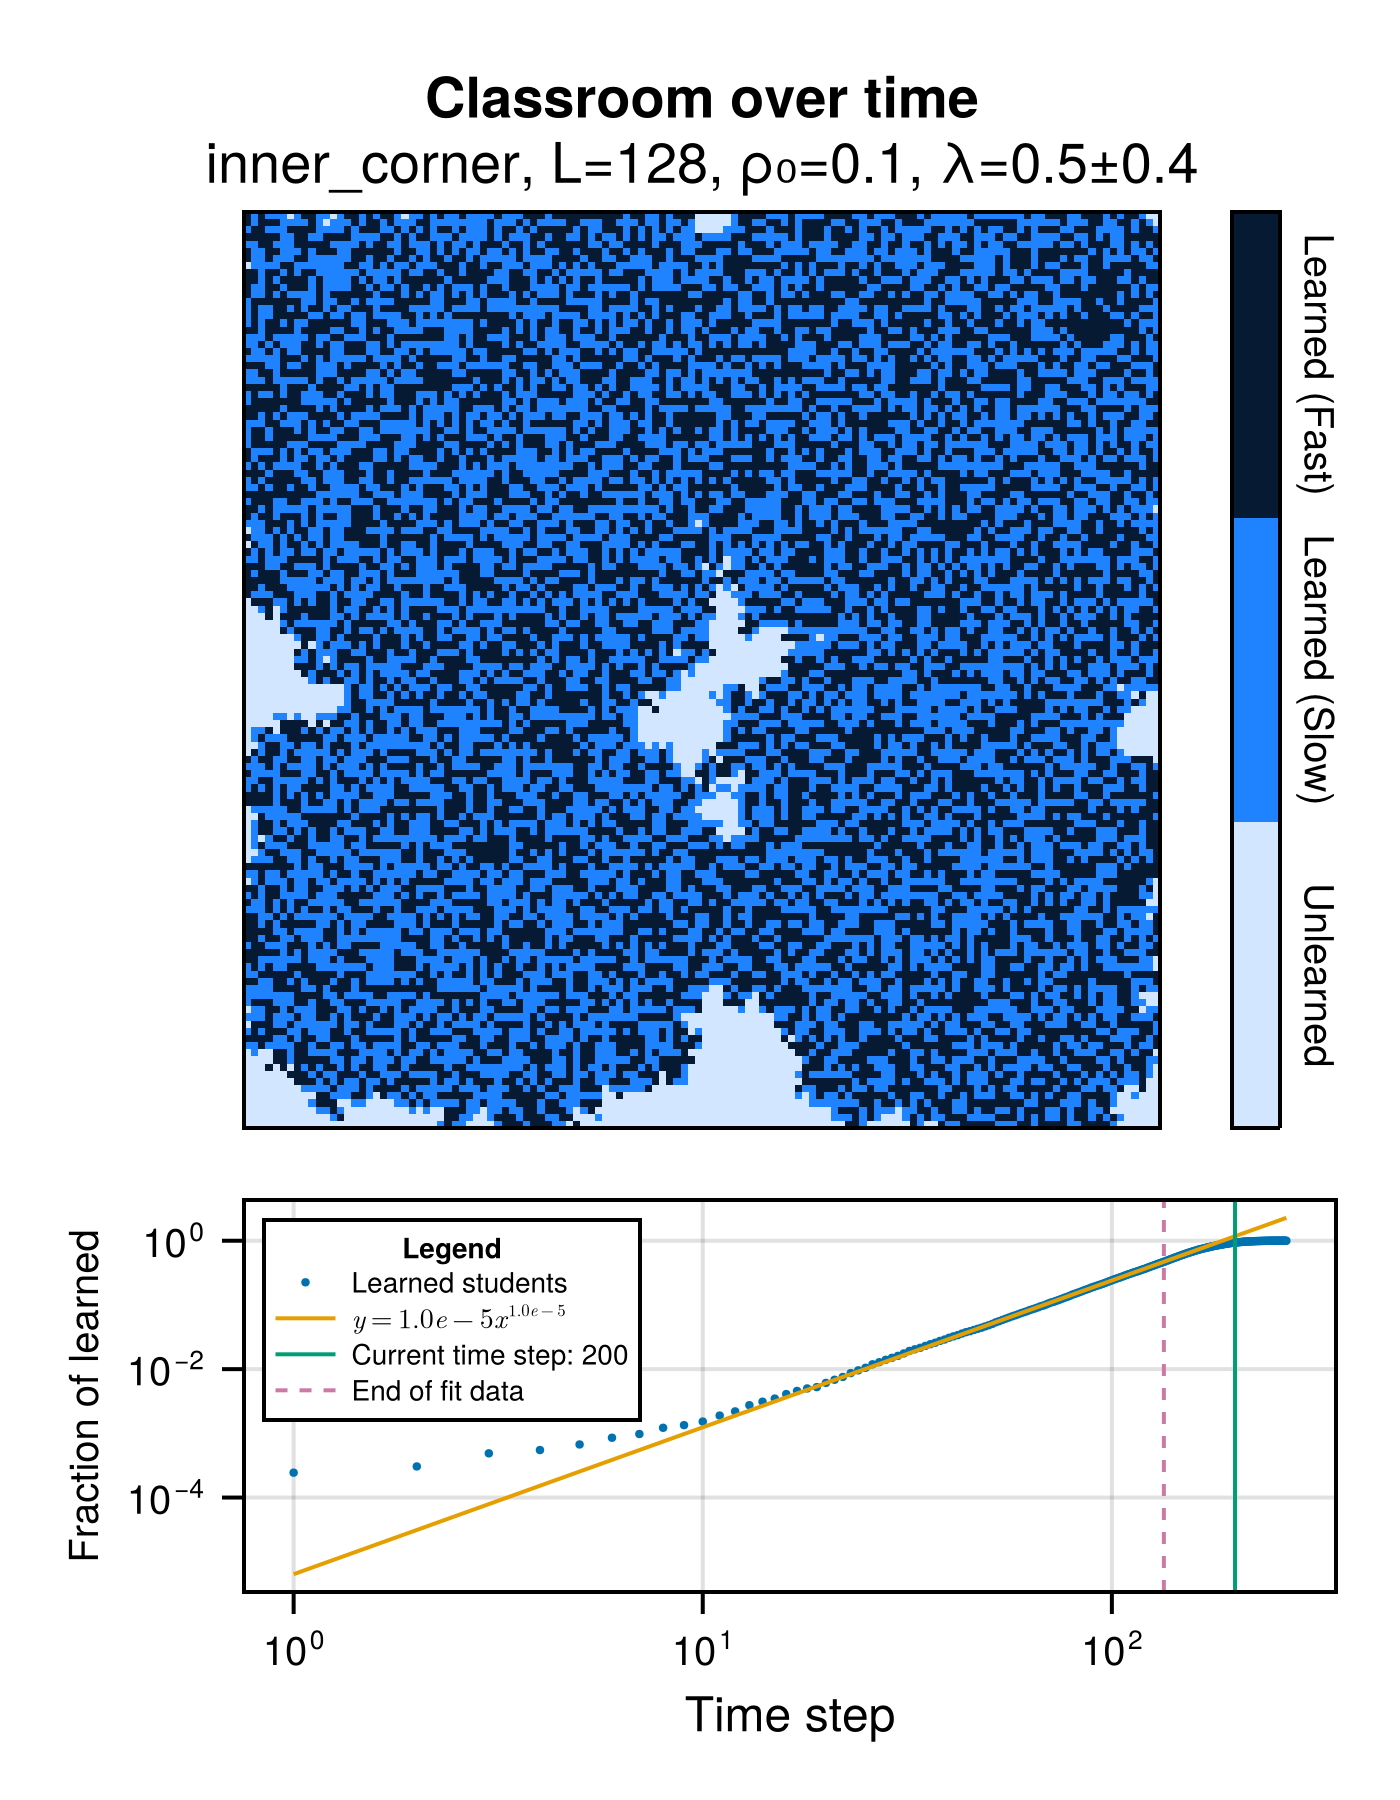
\includegraphics[width=0.40\textwidth]{figures/2D-BPCAIH-analysis/class evolutions/low rho/2DBPCAIH-inner_corner-128-0.1-0.5-0.4-trial_3-200.png}}
   \caption{Sample classroom evolutions for PI with the inner corner SA with $L=128$ at different times $t$ for positional learning coefficient $\rho_0=0.1$, $\delta\lambda = 0.4$.
   Dark blue squares represent learned students with learning rate $\lambda = \lambda_0 + \delta\lambda$, blue squares represent learned students with learning rate $\lambda = \lambda_0 - \delta\lambda$, and light blue squares represent unlearned students.
   The accompanying graph shows the fraction of learned students as a function time step.
   The blue dots represent data points. 
   The yellow line shows the power law fit.
   The pink dashed vertical line shows where we truncate the data for fitting the power law.
   The green vertical line shows the current time step in the simulation.
   }
   \label{fig:2DBPCAIH sample class evolution low rho}
\end{figure}

\begin{figure}[htbp!]
   \centering
   \subfigure[$t=5$]{\label{fig:2DBPCAIH class evolution high rho 5}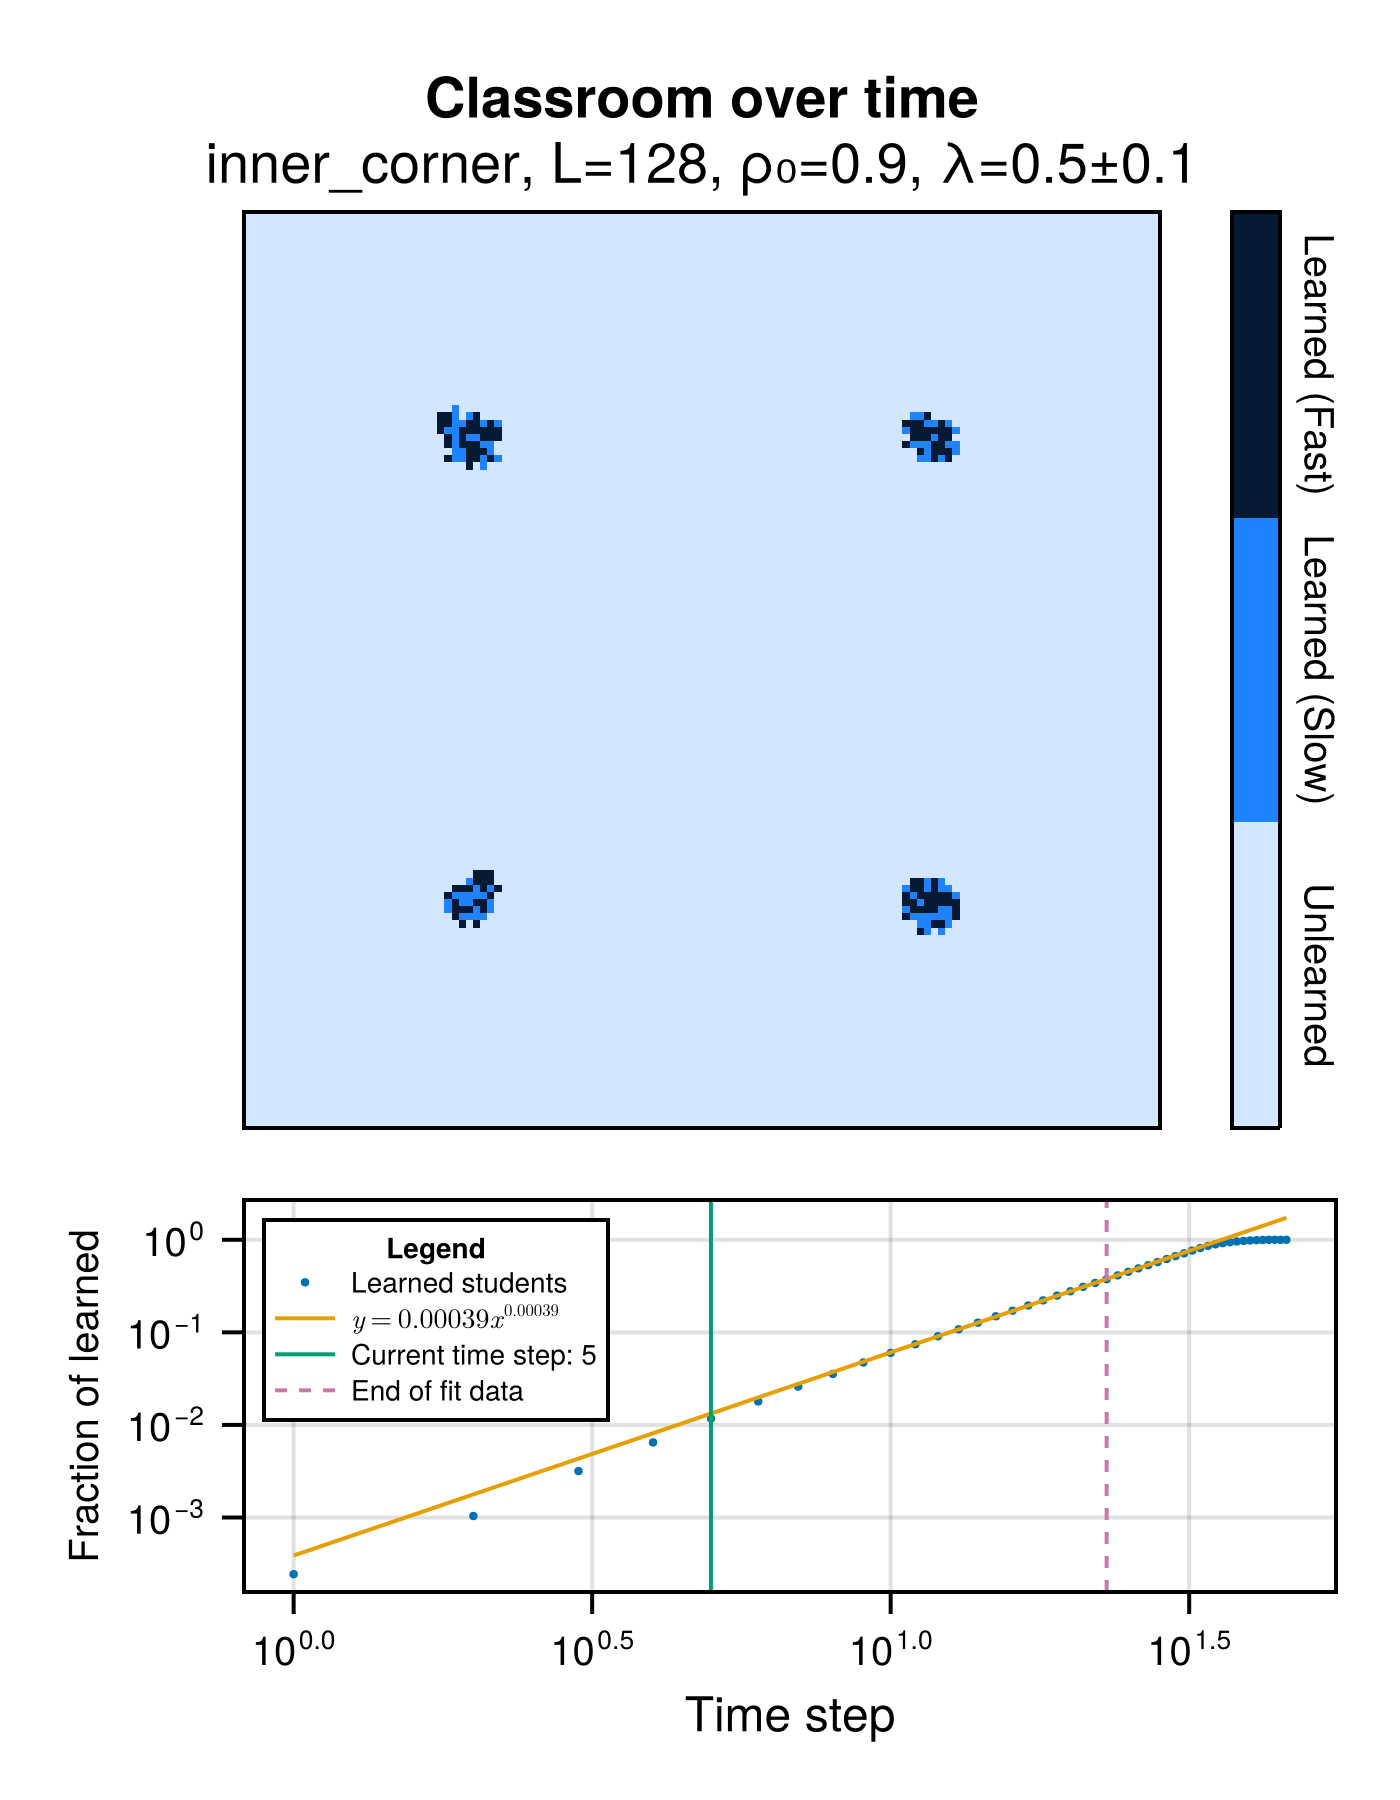
\includegraphics[width=0.40\textwidth]{figures/2D-BPCAIH-analysis/class evolutions/high rho/2DBPCAIH-inner_corner-128-0.9-0.5-0.1-trial_3-5.png}}
   \subfigure[$t=16$]{\label{fig:2DBPCAIH class evolution high rho 16}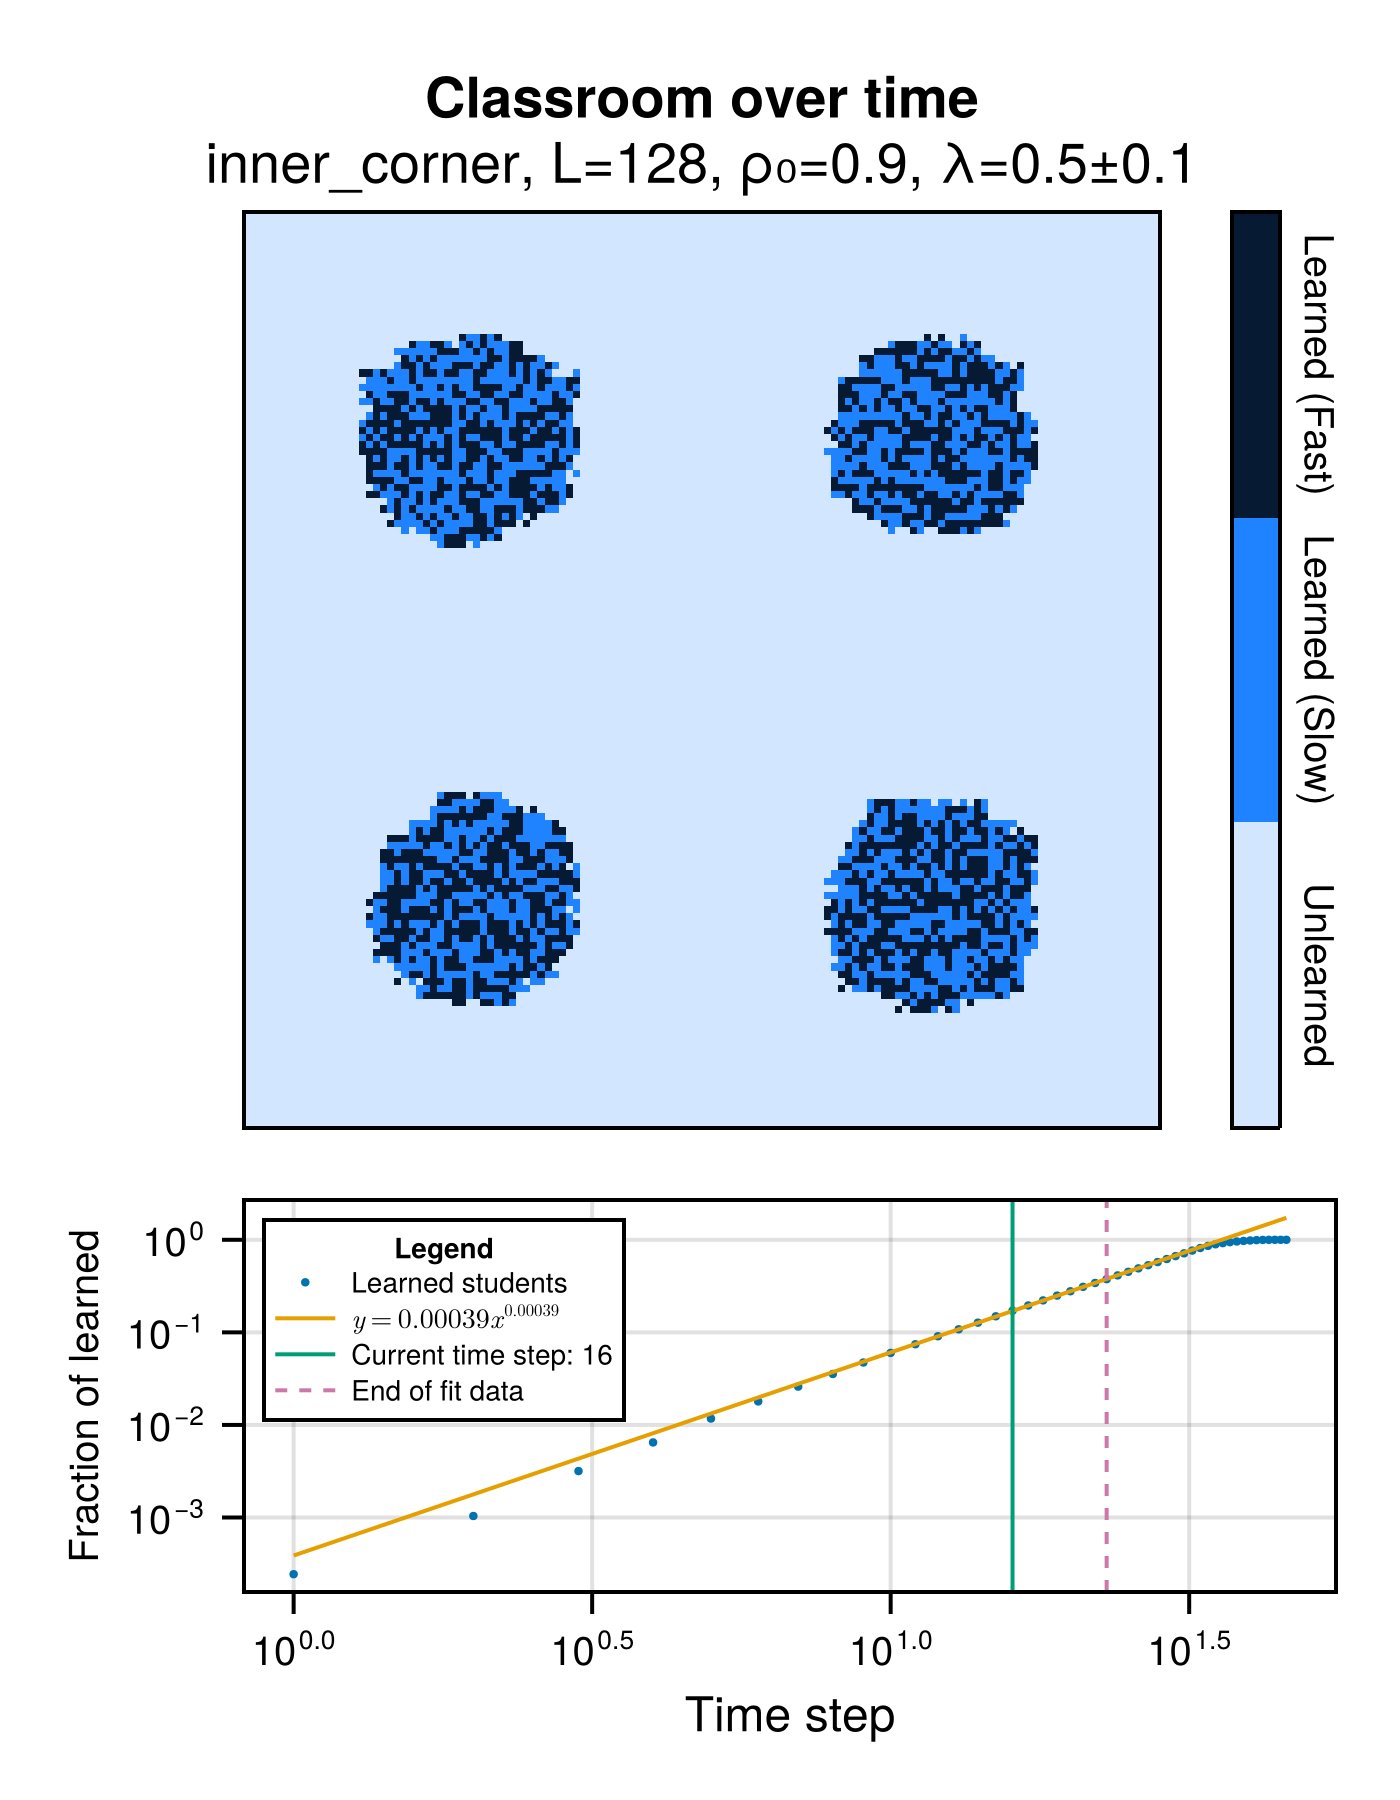
\includegraphics[width=0.40\textwidth]{figures/2D-BPCAIH-analysis/class evolutions/high rho/2DBPCAIH-inner_corner-128-0.9-0.5-0.1-trial_3-16.png}}
   \subfigure[$t=30$]{\label{fig:2DBPCAIH class evolution high rho 30}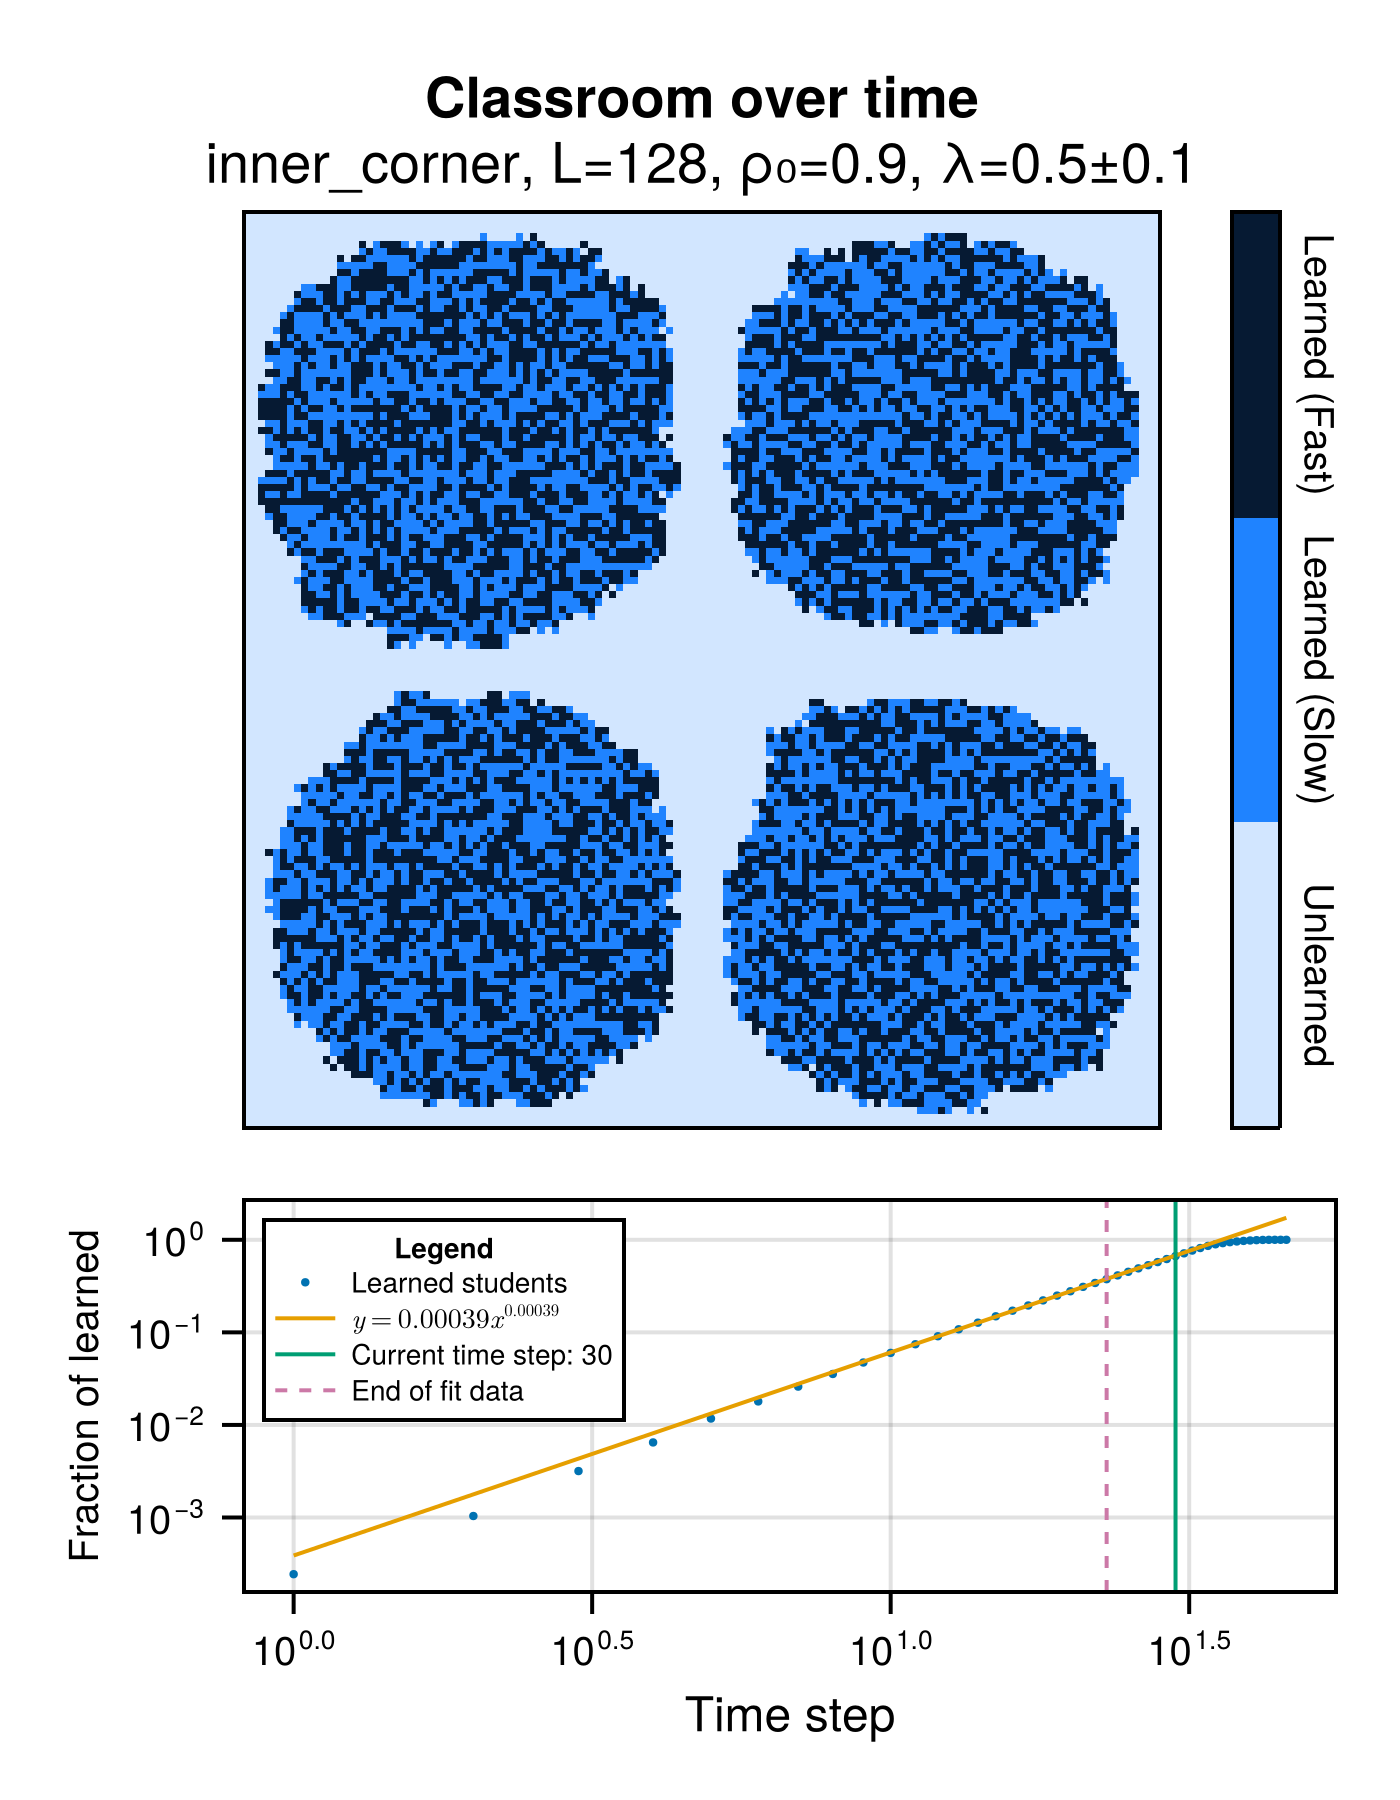
\includegraphics[width=0.40\textwidth]{figures/2D-BPCAIH-analysis/class evolutions/high rho/2DBPCAIH-inner_corner-128-0.9-0.5-0.1-trial_3-30.png}}
   \subfigure[$t=36$]{\label{fig:2DBPCAIH class evolution high rho 36}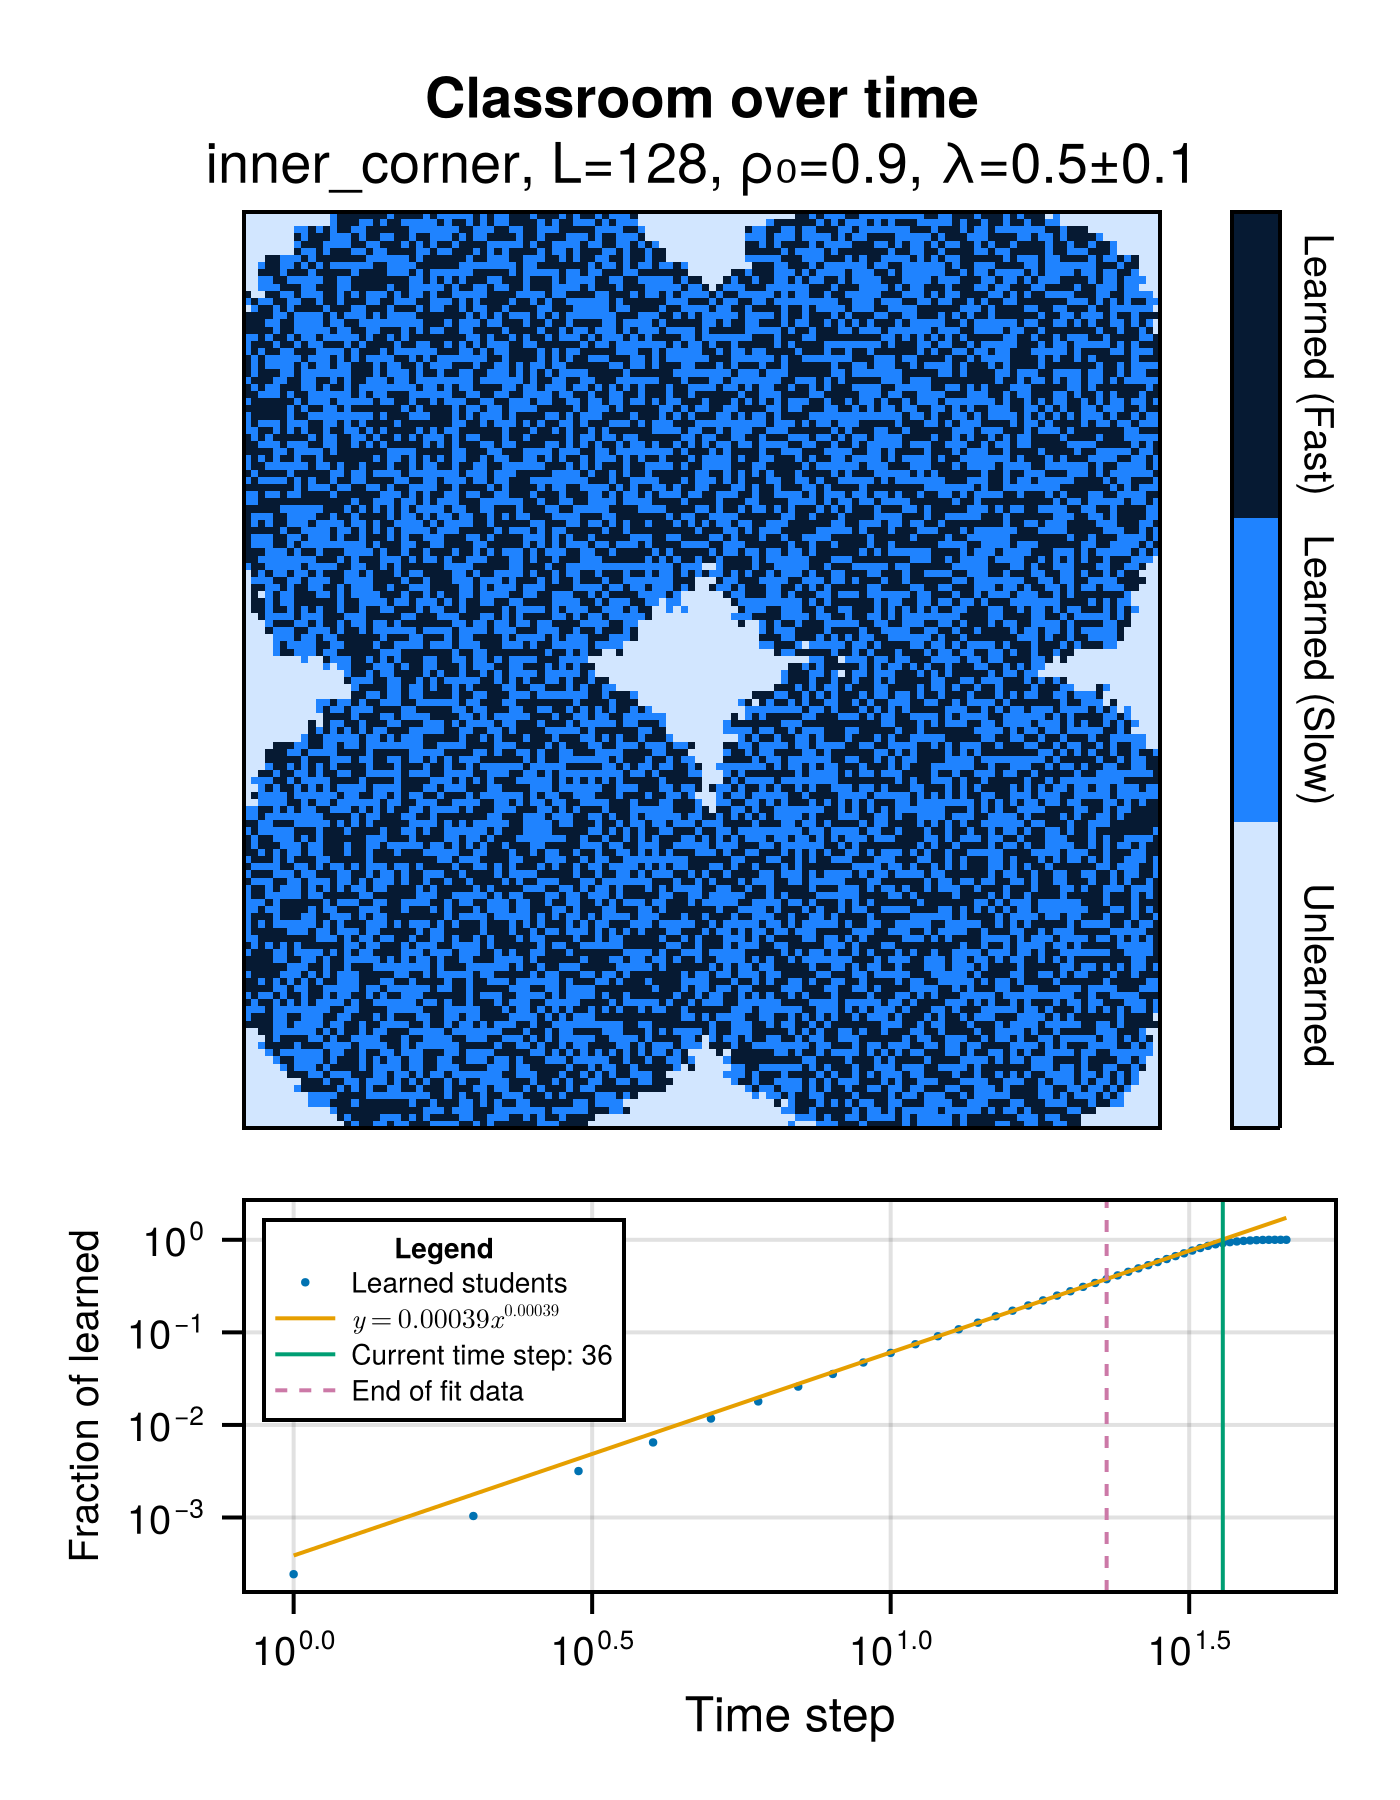
\includegraphics[width=0.40\textwidth]{figures/2D-BPCAIH-analysis/class evolutions/high rho/2DBPCAIH-inner_corner-128-0.9-0.5-0.1-trial_3-36.png}}   
   \caption{Sample classroom evolutions for PI with the inner corner SA with $L=128$ at different times $t$ for positional learning coefficient $\rho_0=0.9$, $\delta\lambda = 0.1$.
   Dark blue squares represent learned students with learning rate $\lambda = \lambda_0 + \delta\lambda$, blue squares represent learned students with learning rate $\lambda = \lambda_0 - \delta\lambda$, and light blue squares represent unlearned students.
   The accompanying graph shows the fraction of learned students as a function time step.
   The blue dots represent data points. 
   The yellow line shows the power law fit.
   The pink dashed vertical line shows where we truncate the data for fitting the power law.
   The green vertical line shows the current time step in the simulation.
   }
   \label{fig:2DBPCAIH sample class evolution high rho}
\end{figure}

\begin{figure}[htbp!]
   \centering
   \subfigure[$t=5$]{\label{fig:2DBPCAIH class evolution high rho high delta 5}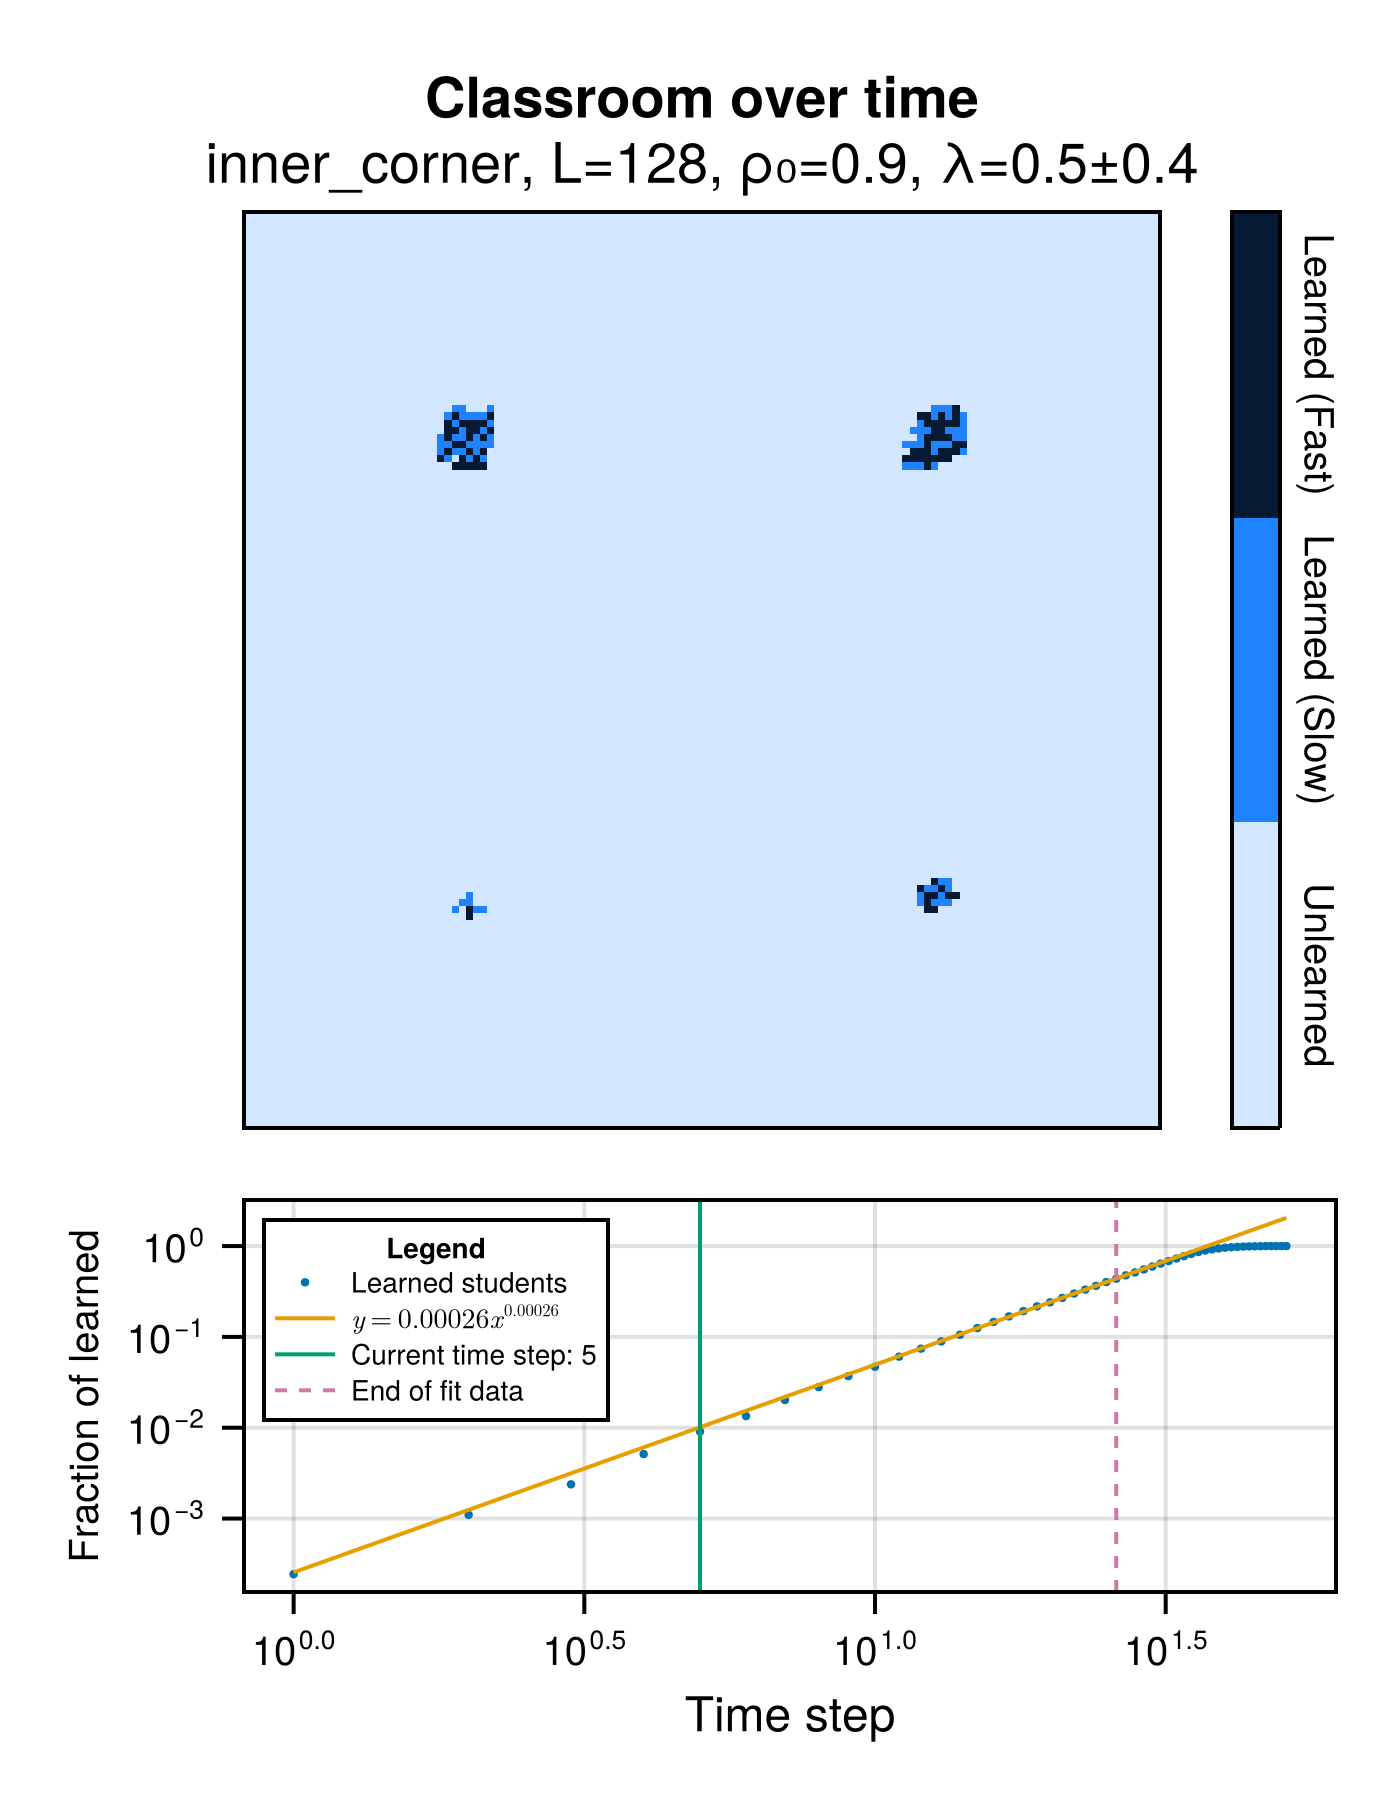
\includegraphics[width=0.40\textwidth]{figures/2D-BPCAIH-analysis/class evolutions/high rho high delta/2DBPCAIH-inner_corner-128-0.9-0.5-0.4-trial_3-5.png}}
   \subfigure[$t=13$]{\label{fig:2DBPCAIH class evolution high rho high delta 13}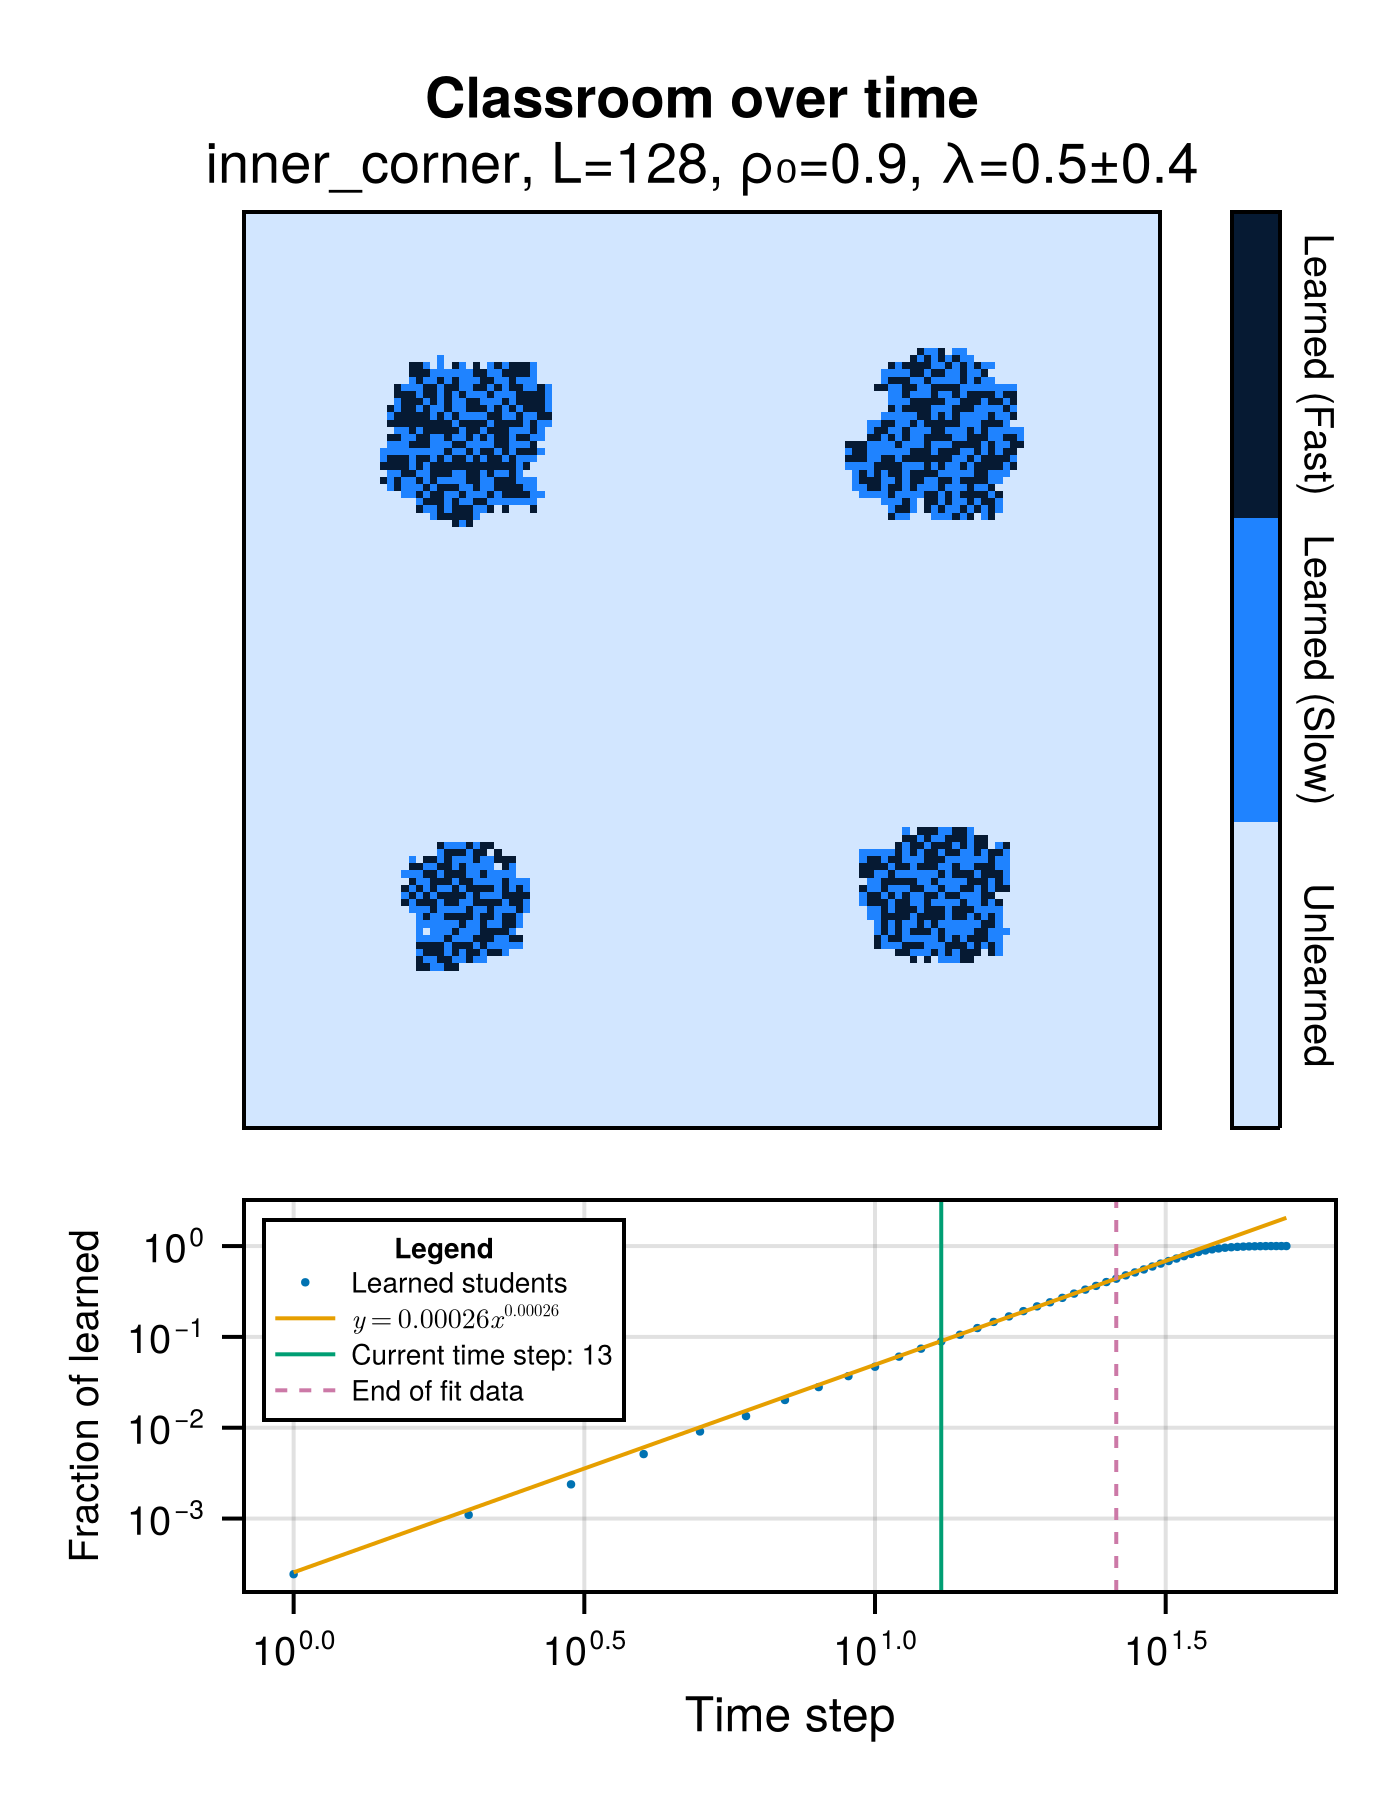
\includegraphics[width=0.40\textwidth]{figures/2D-BPCAIH-analysis/class evolutions/high rho high delta/2DBPCAIH-inner_corner-128-0.9-0.5-0.4-trial_3-13.png}}
   \subfigure[$t=19$]{\label{fig:2DBPCAIH class evolution high rho high delta 19}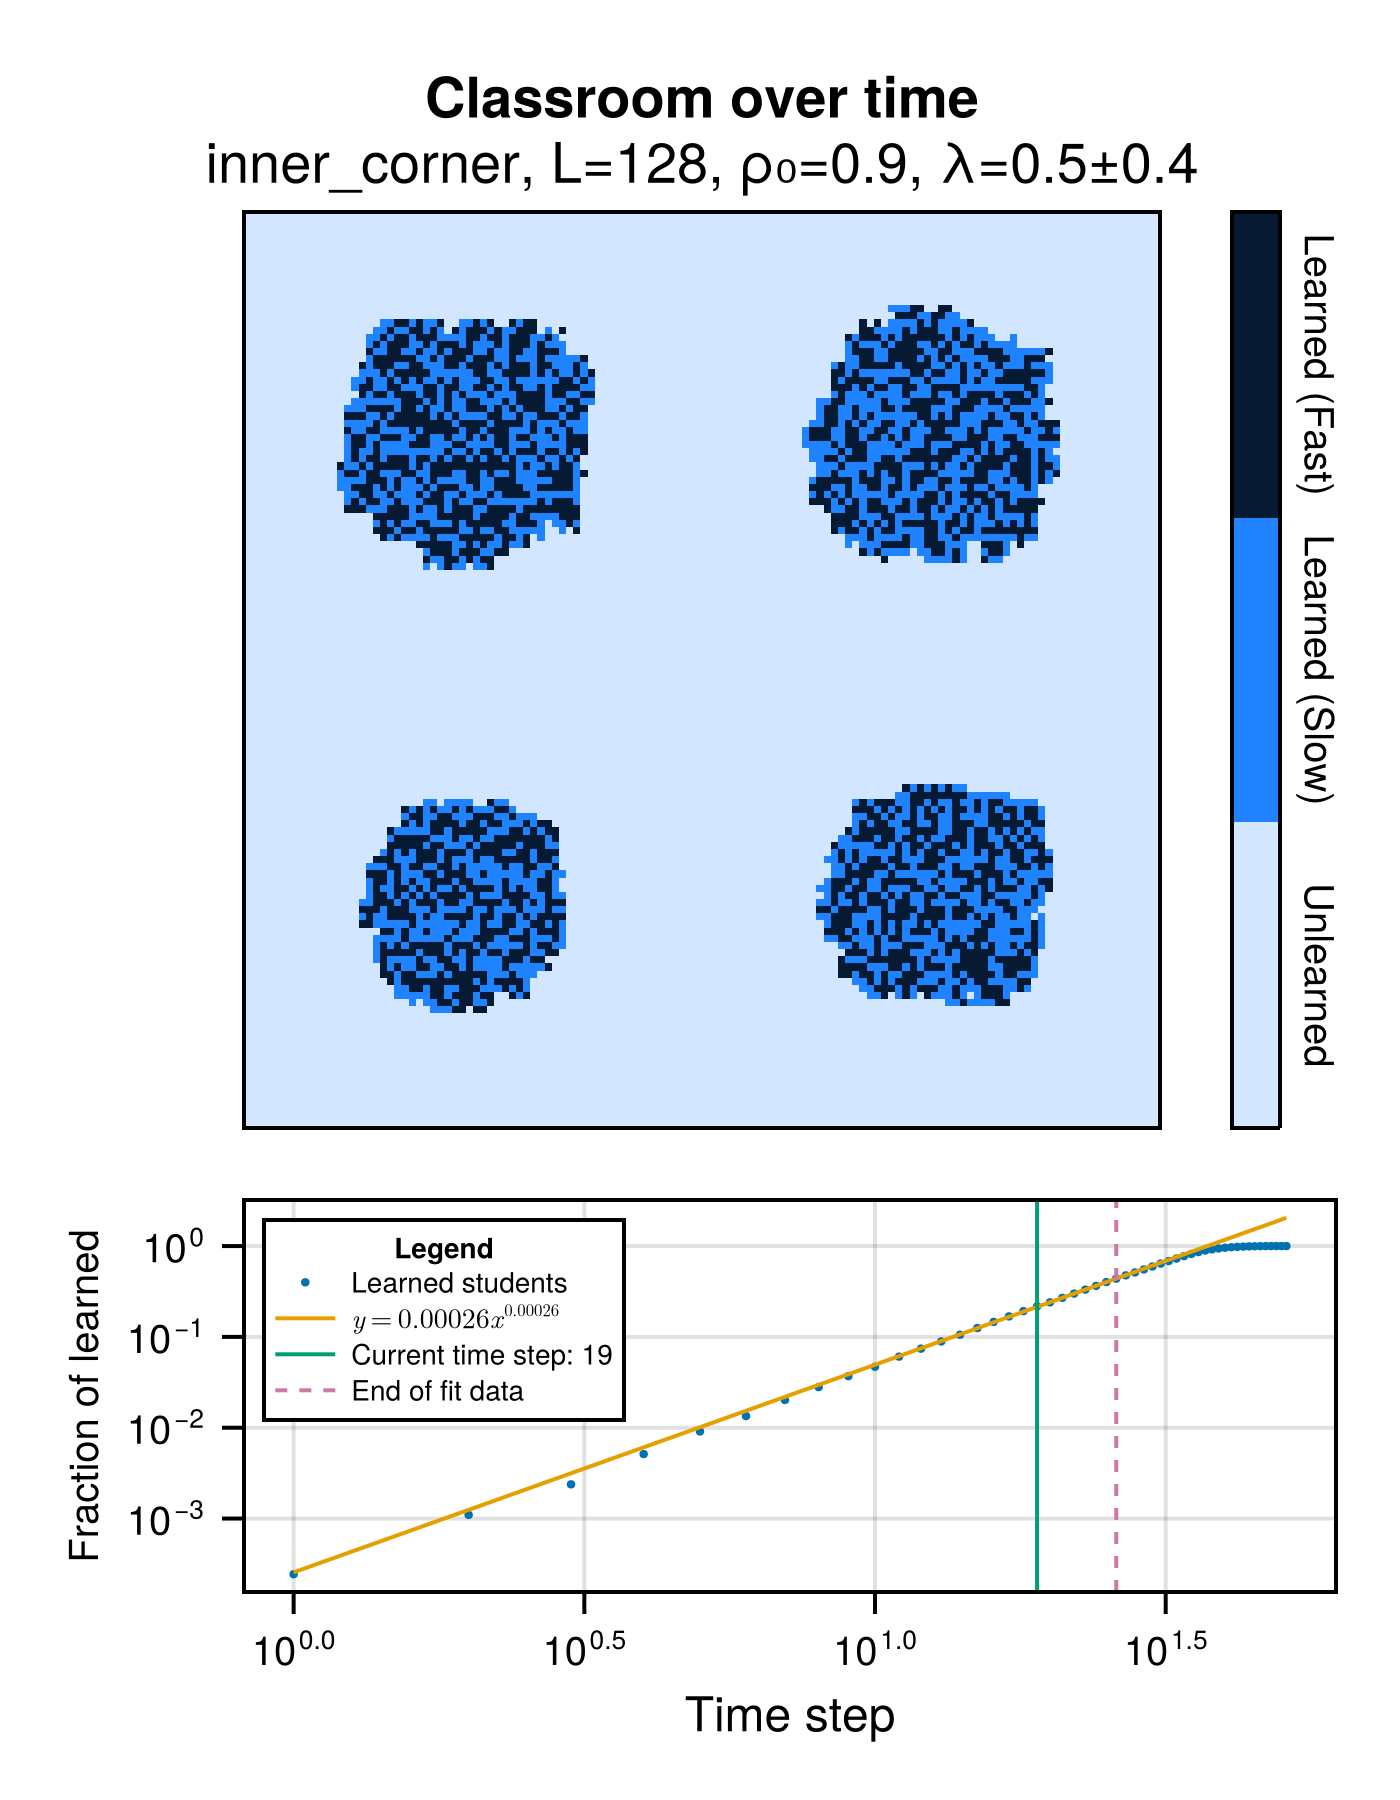
\includegraphics[width=0.40\textwidth]{figures/2D-BPCAIH-analysis/class evolutions/high rho high delta/2DBPCAIH-inner_corner-128-0.9-0.5-0.4-trial_3-19.png}}
   \subfigure[$t=29$]{\label{fig:2DBPCAIH class evolution high rho high delta 29}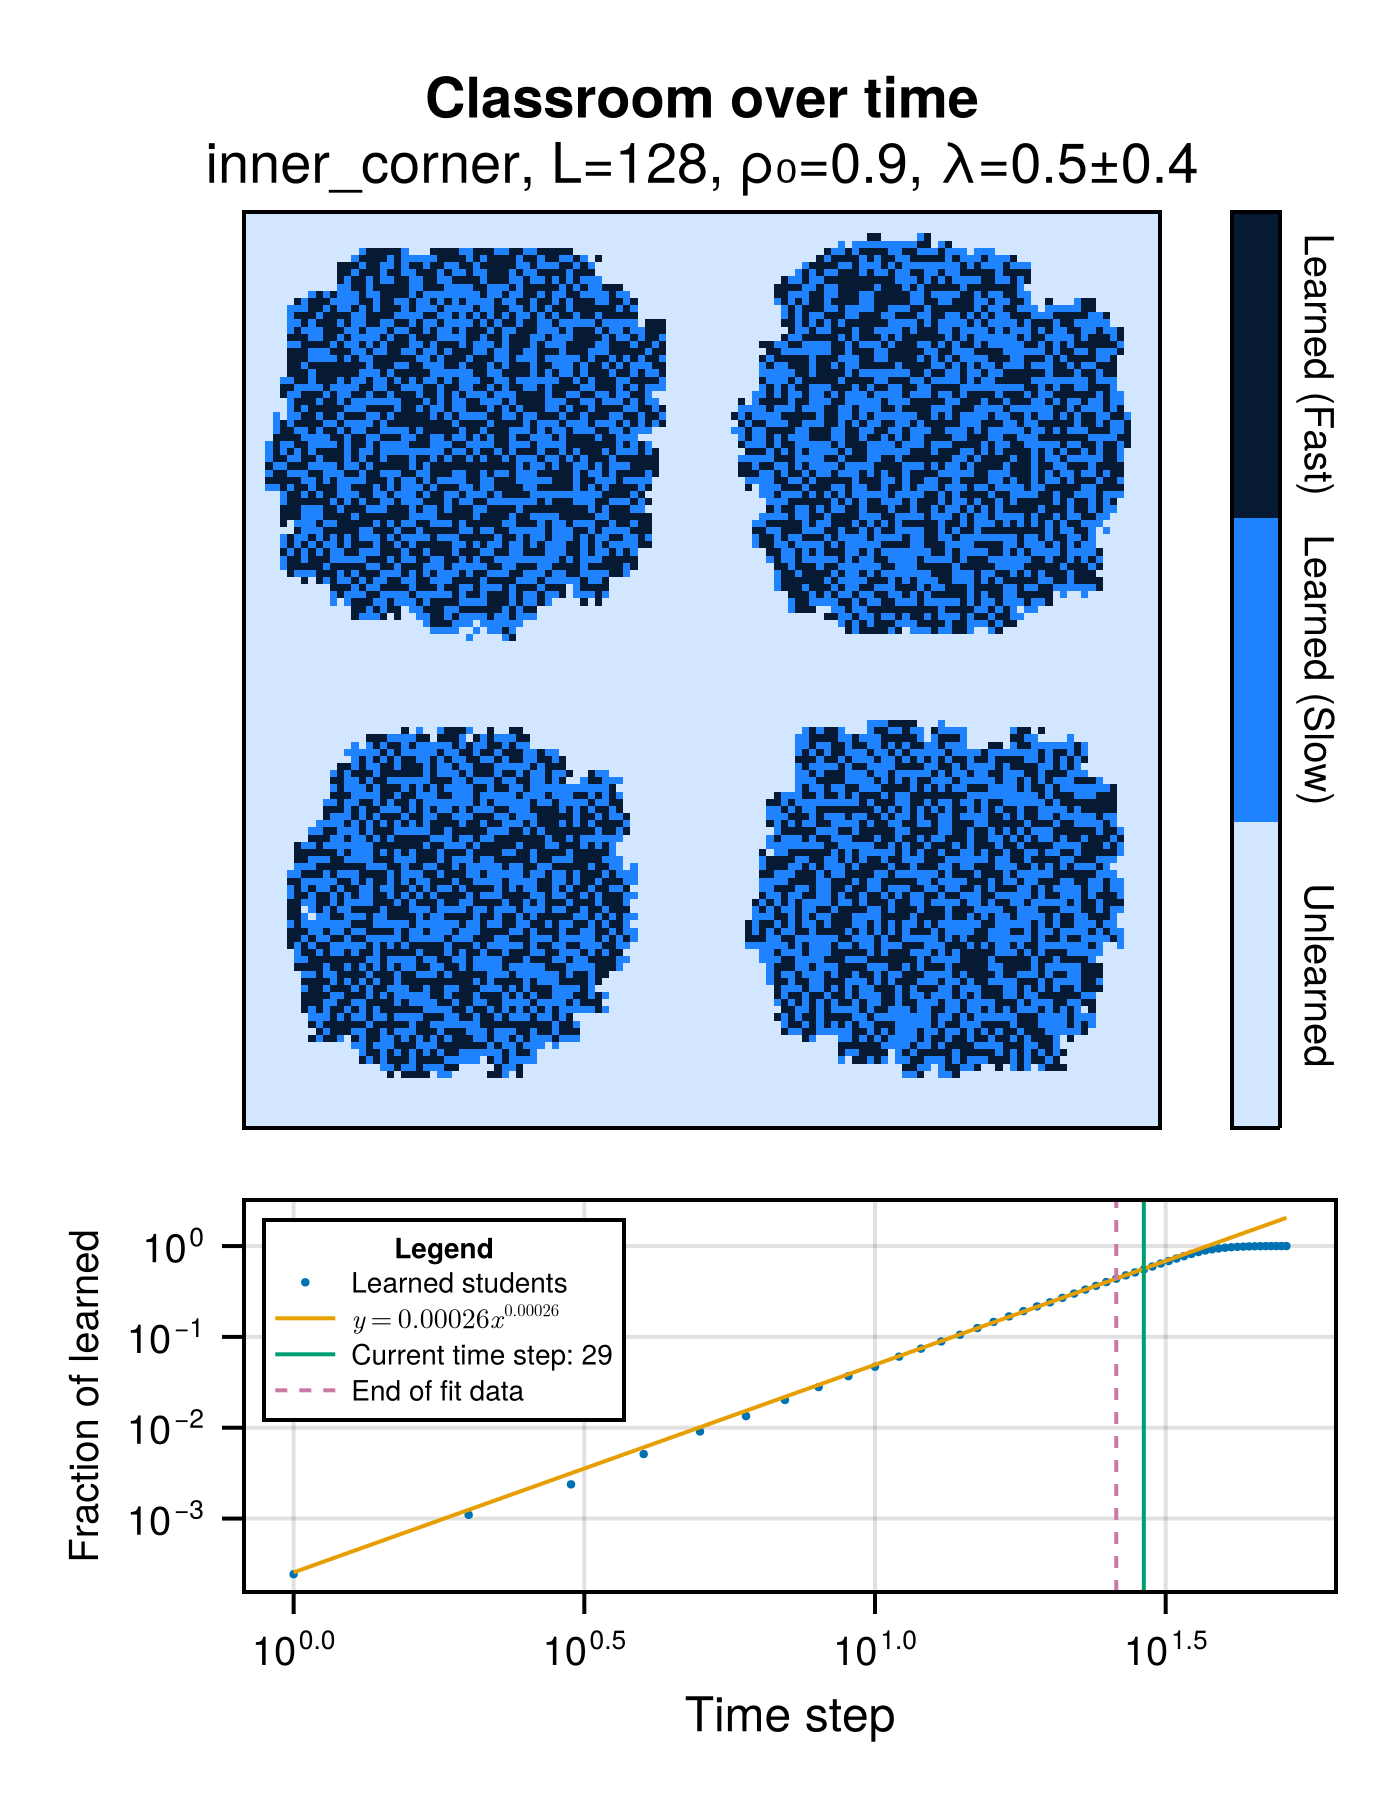
\includegraphics[width=0.40\textwidth]{figures/2D-BPCAIH-analysis/class evolutions/high rho high delta/2DBPCAIH-inner_corner-128-0.9-0.5-0.4-trial_3-29.png}}
   \caption{Sample classroom evolutions for PI with the inner corner SA with $L=128$ at different times $t$ for positional learning rate $\rho_0=0.9$, $\delta\lambda = 0.4$.
   Dark blue squares represent learned students with learning rate $\lambda = \lambda_0 + \delta\lambda$, blue squares represent learned students with learning rate $\lambda = \lambda_0 - \delta\lambda$, and light blue squares represent unlearned students.
   The accompanying graph shows the fraction of learned students as a function time step.
   The blue dots represent data points. 
   The yellow line shows the power law fit.
   The pink dashed vertical line shows where we truncate the data for fitting the power law.
   The green vertical line shows the current time step in the simulation.
   }
   \label{fig:2DBPCAIH sample class evolution high rho high delta}
\end{figure}

\subsection{Traditional Instruction}
For traditional instructon, even though the value of positional learning coefficient $\rho_0$ is still an important factor in determininng class performance, the effect of $\delta\lambda$ is more pronounced compared to PI.
The trend we see in traditional instruction that is absent or less evident in PI, is that majority of the students that learn earlier in the simulations are fast learning students students (Figure~\ref{fig:2DBPCAIH class evolution trad low rho high delta 2}). 
After this period, most of the simulation time is spent waiting for the slow learning students to learn.
This behavior is more pronounced for higher values of $\delta\lambda$ and lower values of $\rho_0$ as shown in Figure~\ref{fig:2DBPCAIH sample class evolution trad low rho high delta}.
This could explain the deviation from the power law fit at earlier times $t$ for the traditional model considering that the deviation shows that the class learning rate is higher than the fitted power law.

\begin{figure}[htbp!]
   \centering
   \subfigure[$t=2$]{\label{fig:2DBPCAIH class evolution trad low rho high delta 2}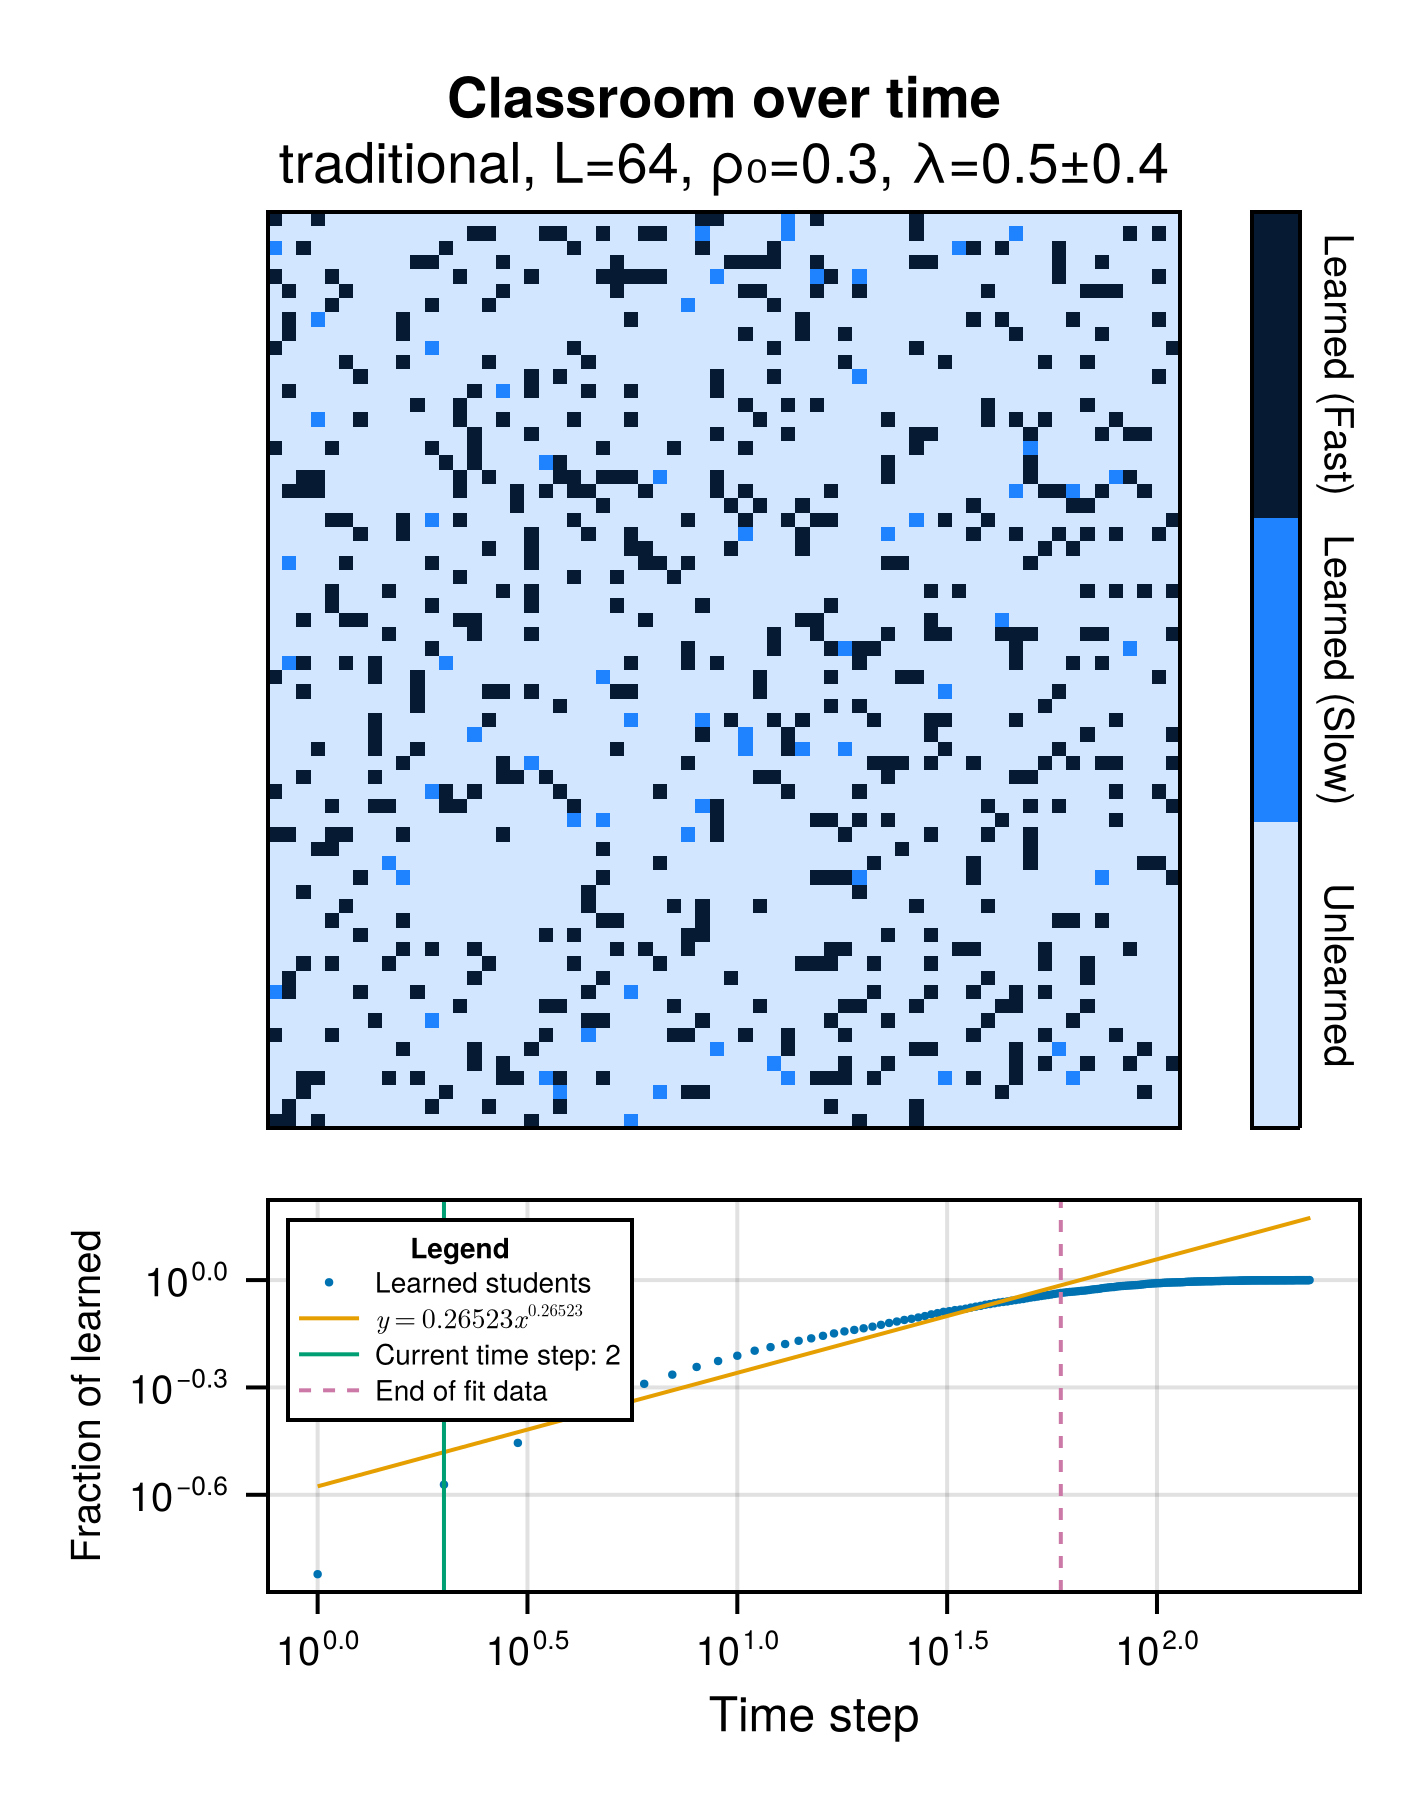
\includegraphics[width=0.40\textwidth]{figures/2D-BPCAIH-analysis/class evolutions/trad low rho high delta/2DBPCAIH-traditional-64-0.3-0.5-0.4-trial_3-2.png}}
   \subfigure[$t=13$]{\label{fig:2DBPCAIH class evolution trad low rho high delta 13}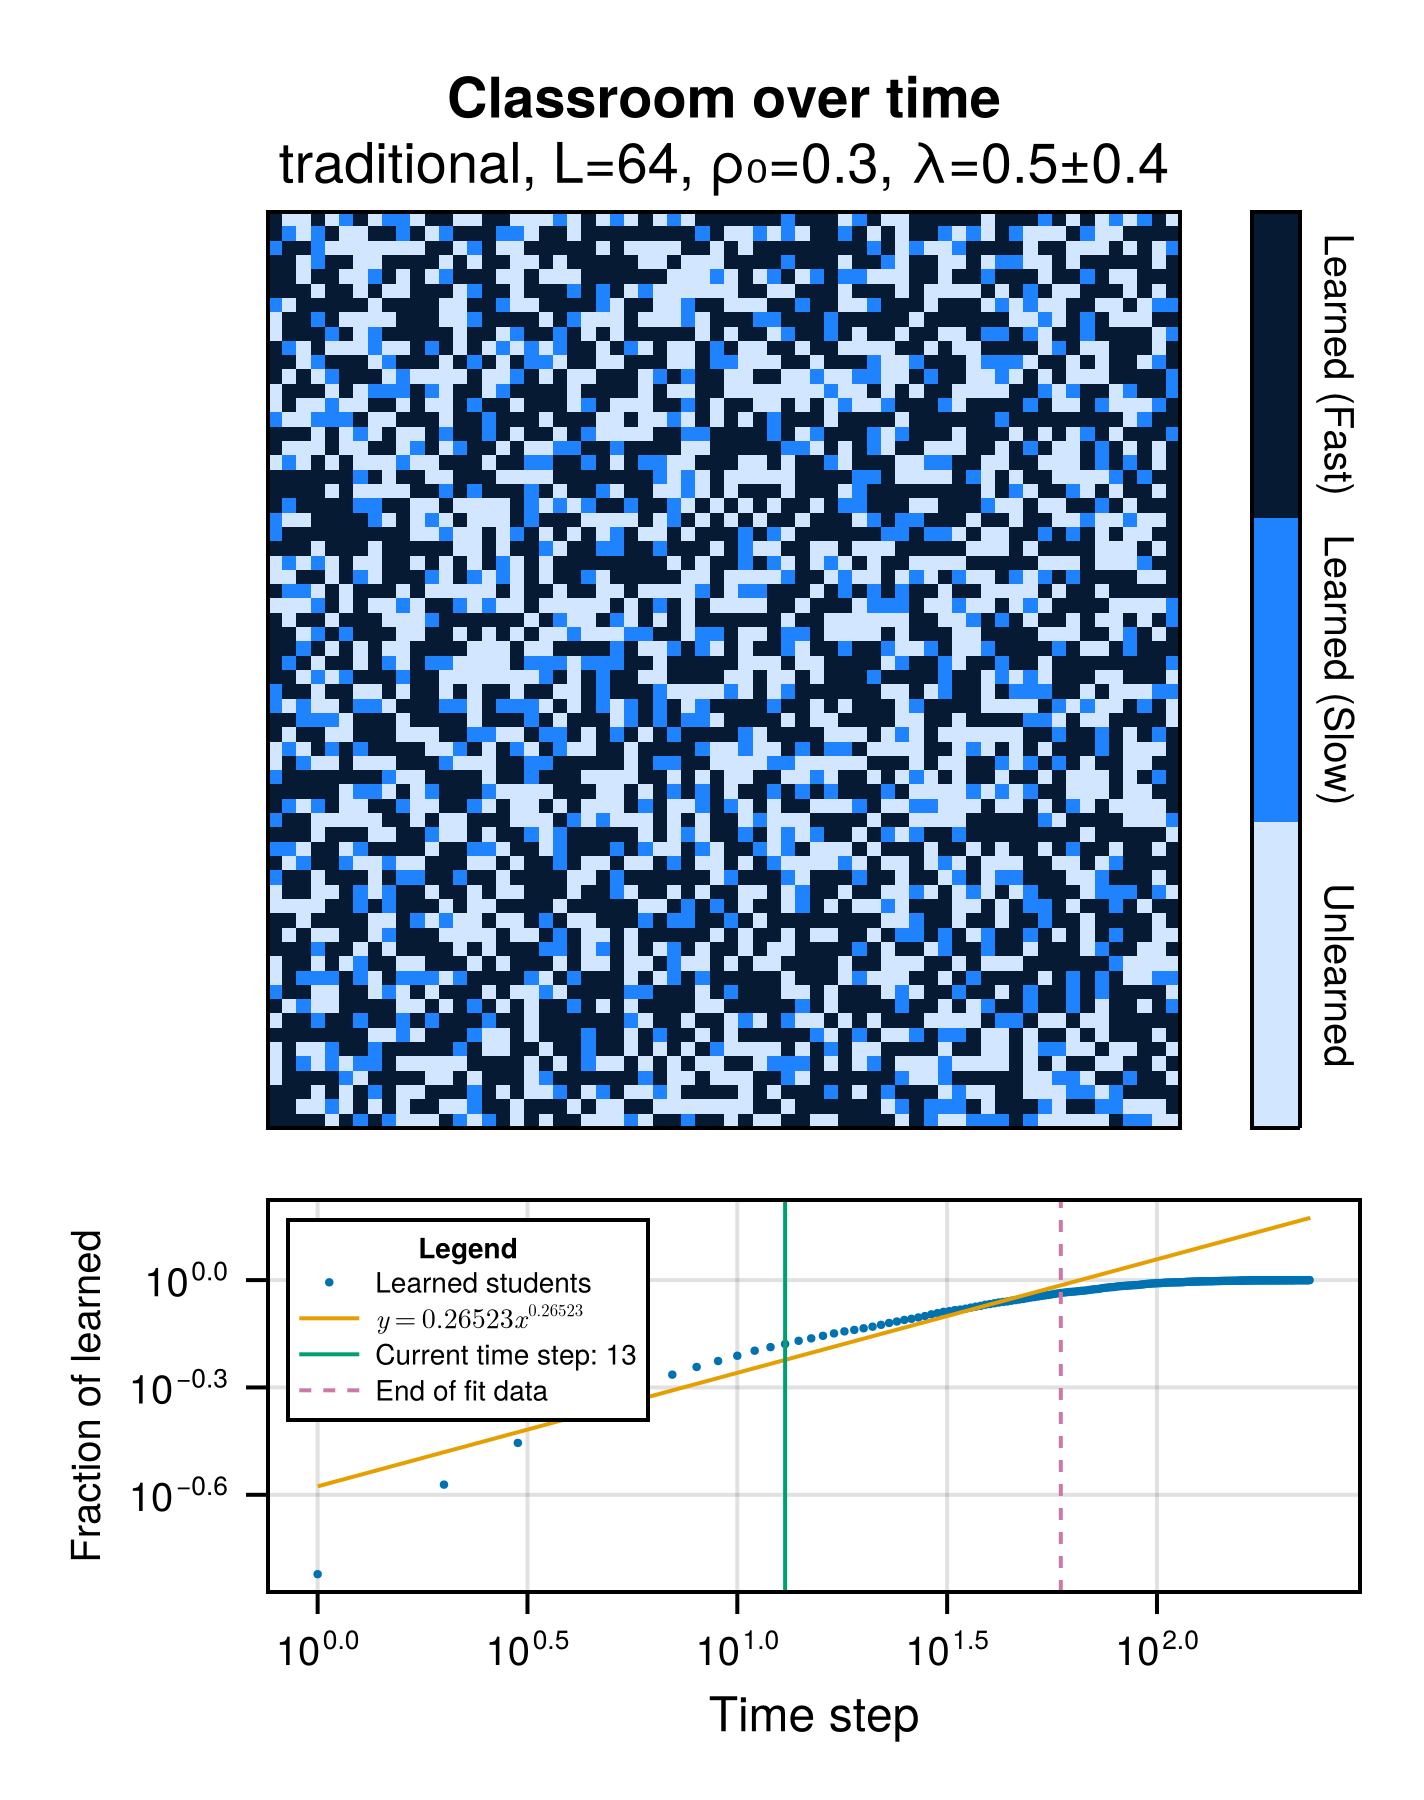
\includegraphics[width=0.40\textwidth]{figures/2D-BPCAIH-analysis/class evolutions/trad low rho high delta/2DBPCAIH-traditional-64-0.3-0.5-0.4-trial_3-13.png}}
   \subfigure[$t=50$]{\label{fig:2DBPCAIH class evolution trad low rho high delta 50}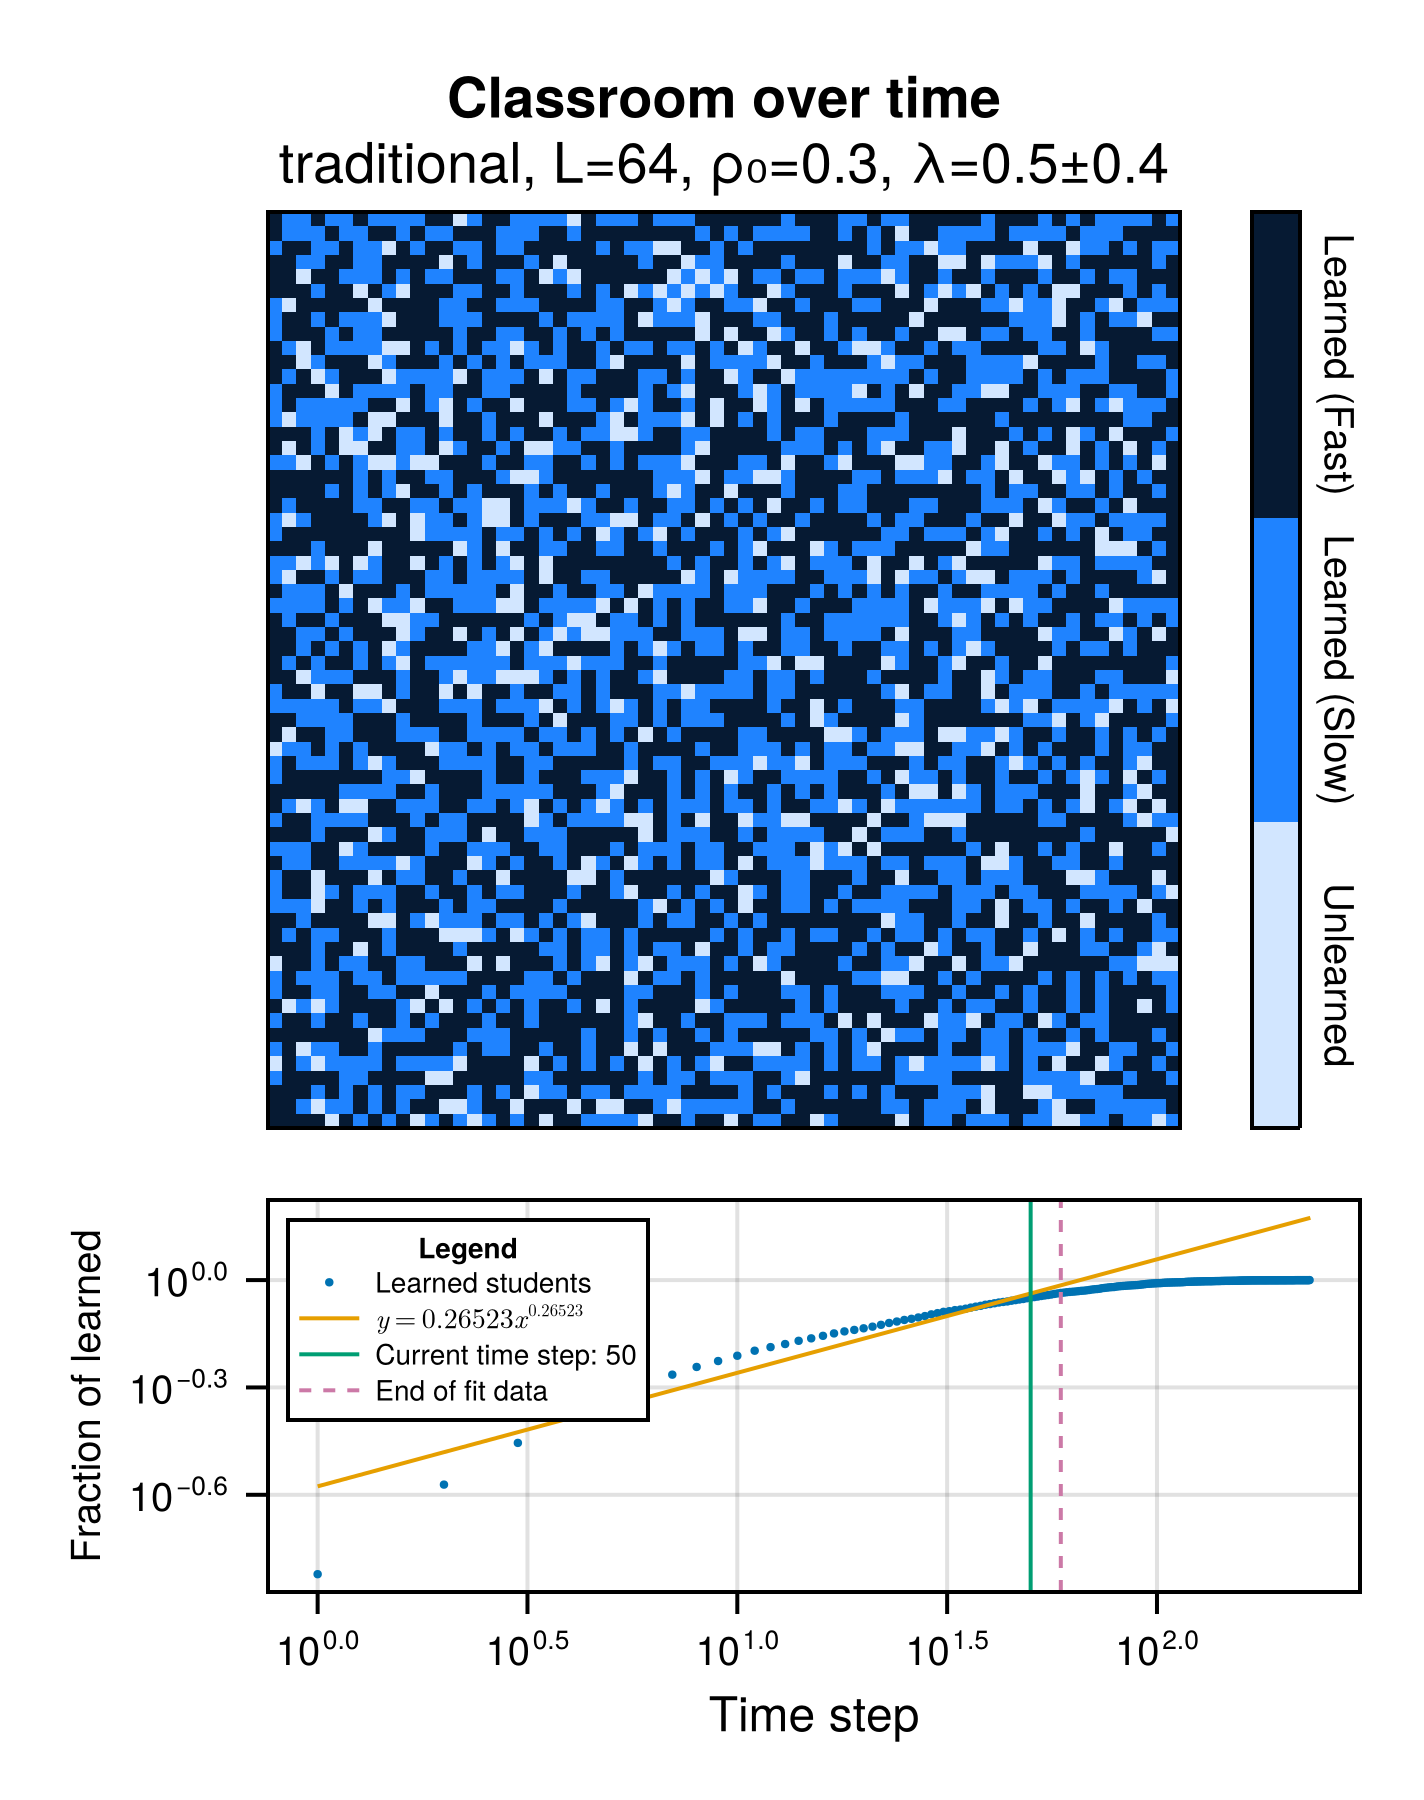
\includegraphics[width=0.40\textwidth]{figures/2D-BPCAIH-analysis/class evolutions/trad low rho high delta/2DBPCAIH-traditional-64-0.3-0.5-0.4-trial_3-50.png}}
   \subfigure[$t=80$]{\label{fig:2DBPCAIH class evolution trad low rho high delta 80}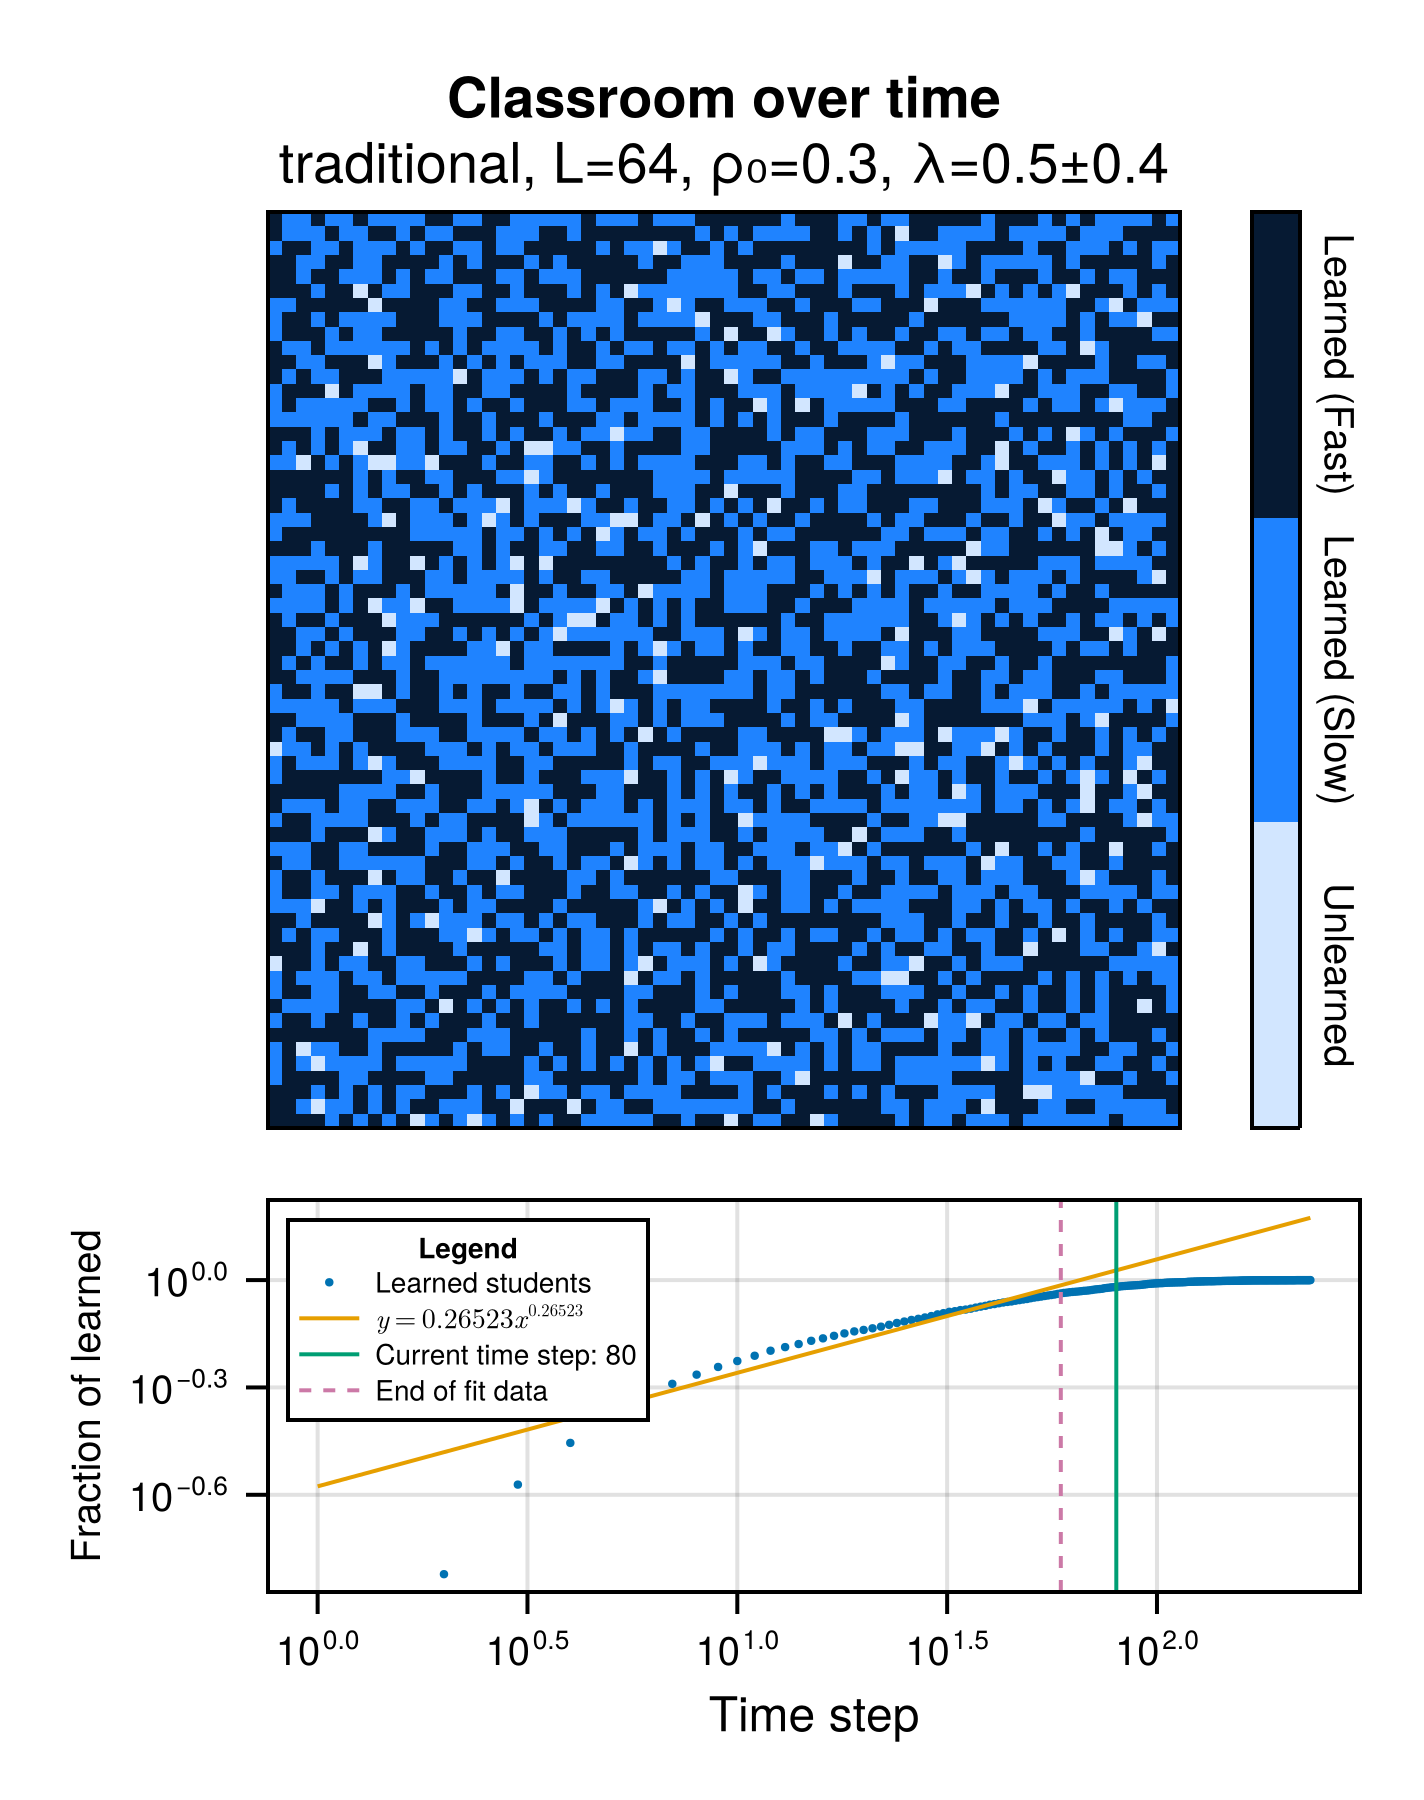
\includegraphics[width=0.40\textwidth]{figures/2D-BPCAIH-analysis/class evolutions/trad low rho high delta/2DBPCAIH-traditional-64-0.3-0.5-0.4-trial_3-80.png}}
   \caption{Sample classroom evolutions for PI with the inner corner SA with $L=128$ at different times $t$ for positional learning coefficient $\rho_0=0.9$, $\delta\lambda = 0.4$.
   Dark blue squares represent learned students with learning rate $\lambda = \lambda_0 + \delta\lambda$, blue squares represent learned students with learning rate $\lambda = \lambda_0 - \delta\lambda$, and light blue squares represent unlearned students.
   The accompanying graph shows the fraction of learned students as a function time step.
   The blue dots represent data points. 
   The yellow line shows the power law fit.
   The pink dashed vertical line shows where we truncate the data for fitting the power law.
   The green vertical line shows the current time step in the simulation.
   }
   \label{fig:2DBPCAIH sample class evolution trad low rho high delta}
\end{figure}

\subsection{Comparing temporal learning dynamics of different classroom configurations}

When varying the class size $N$, as in Figure~\ref{fig:2DBPCAIH t-learned size comparison}, we see that in traditional instruction, the dynamics remains generally unchanged, with only the time to learn $t_{max}$ increasing as the class size $N$ increases. 
For PI, an increase in class size $N$ adds a time delay to when the learning starts to speed up. 
Despite the added time delay, the general shape of the learning curve remains the same.
An increase in class size $N$ also does not affect the time to learn $t_{max}$ for PI as much as it does for the traditional model.

When varying the positional learning factor $\rho_0$, we see that it varies the shape of the learning curve for traditional instruction, especially for lower values of $\rho_0$ as shown in Figure~\ref{fig:2DBPCAIH t-learned rho comparison}. 
For traditional instruction, the value of $\rho_0$ also greatly changes the initial number of students that learn in the second time step.
The same figure shows that for PI, the value of $\rho_0$ has a similar effect to class size $N$, where it only adds a time delay to when the learning starts to speed up.
Notably, the effect of $\rho_0$ is not linear for either instruction models.
We can see in the same figure that those with extremely low values of $\rho$, like that of $\rho_0=0.1$ perform much worse with the learning curves being further from $\rho_0=0.5$ than $\rho_0=0.9$.

Figure~\ref{fig:2DBPCAIH t-learned delta comparison} shows that an increase in heterogeneity $\delta\lambda$ changes how fast the slope of the learning curve changes for the traditional model without changing the initial number of learned students. 
As for PI, an increase in heterogeneity $\delta\lambda$ only affects the learning curve at very high heterogeneity $\delta\lambda$.
The effect of heterogeneity for PI is also similar to the effects of class size $N$ and positional learning factor $\rho_0$ where it only adds a time delay, shifting the learning curve to the right.

As shown in Figure~\ref{fig:2DBPCAIH t-learned SA comparison}, when comparing between the different SA's for PI and traditional instruction, at least for $L=64, \rho_0=0.5, \lambda=0.5\pm0.2$, traditional instruction generally performs better than PI, especially in the early time steps. 
Among the different SA's for PI, the inner corner SA still performs the best while the center and outer corner SAs perform similarly, the same conclusion we got from the homogenous case.
Contrary to the results of the homoegnous classes, the random SA did not perform the worst, it performed better than the center and outer corner SA's.

One observation that is consistent with all the comparisons shown in Figure~\ref{fig:2DBPCAIH t-learned comparisons} is that even though using traditional instruction has more students learning in the early time steps, it also spend more time waiting for the last few students to learn. 
In contrast to this, PI takes some time before the learning starts to speed up, but once majority of the students have learned, it does not take long until all the students to learn.
This makes PI have a shorter time to learn $t_{max}$, despite being outperformed by the traditional model in early time steps.
This phenomenon is further investigated in the next sections where we look closer at the different factors that can affect which set up is better for different classroom parameters.

\begin{figure}[htbp!]
   \centering
   \subfigure[Size comparison]{\label{fig:2DBPCAIH t-learned size comparison}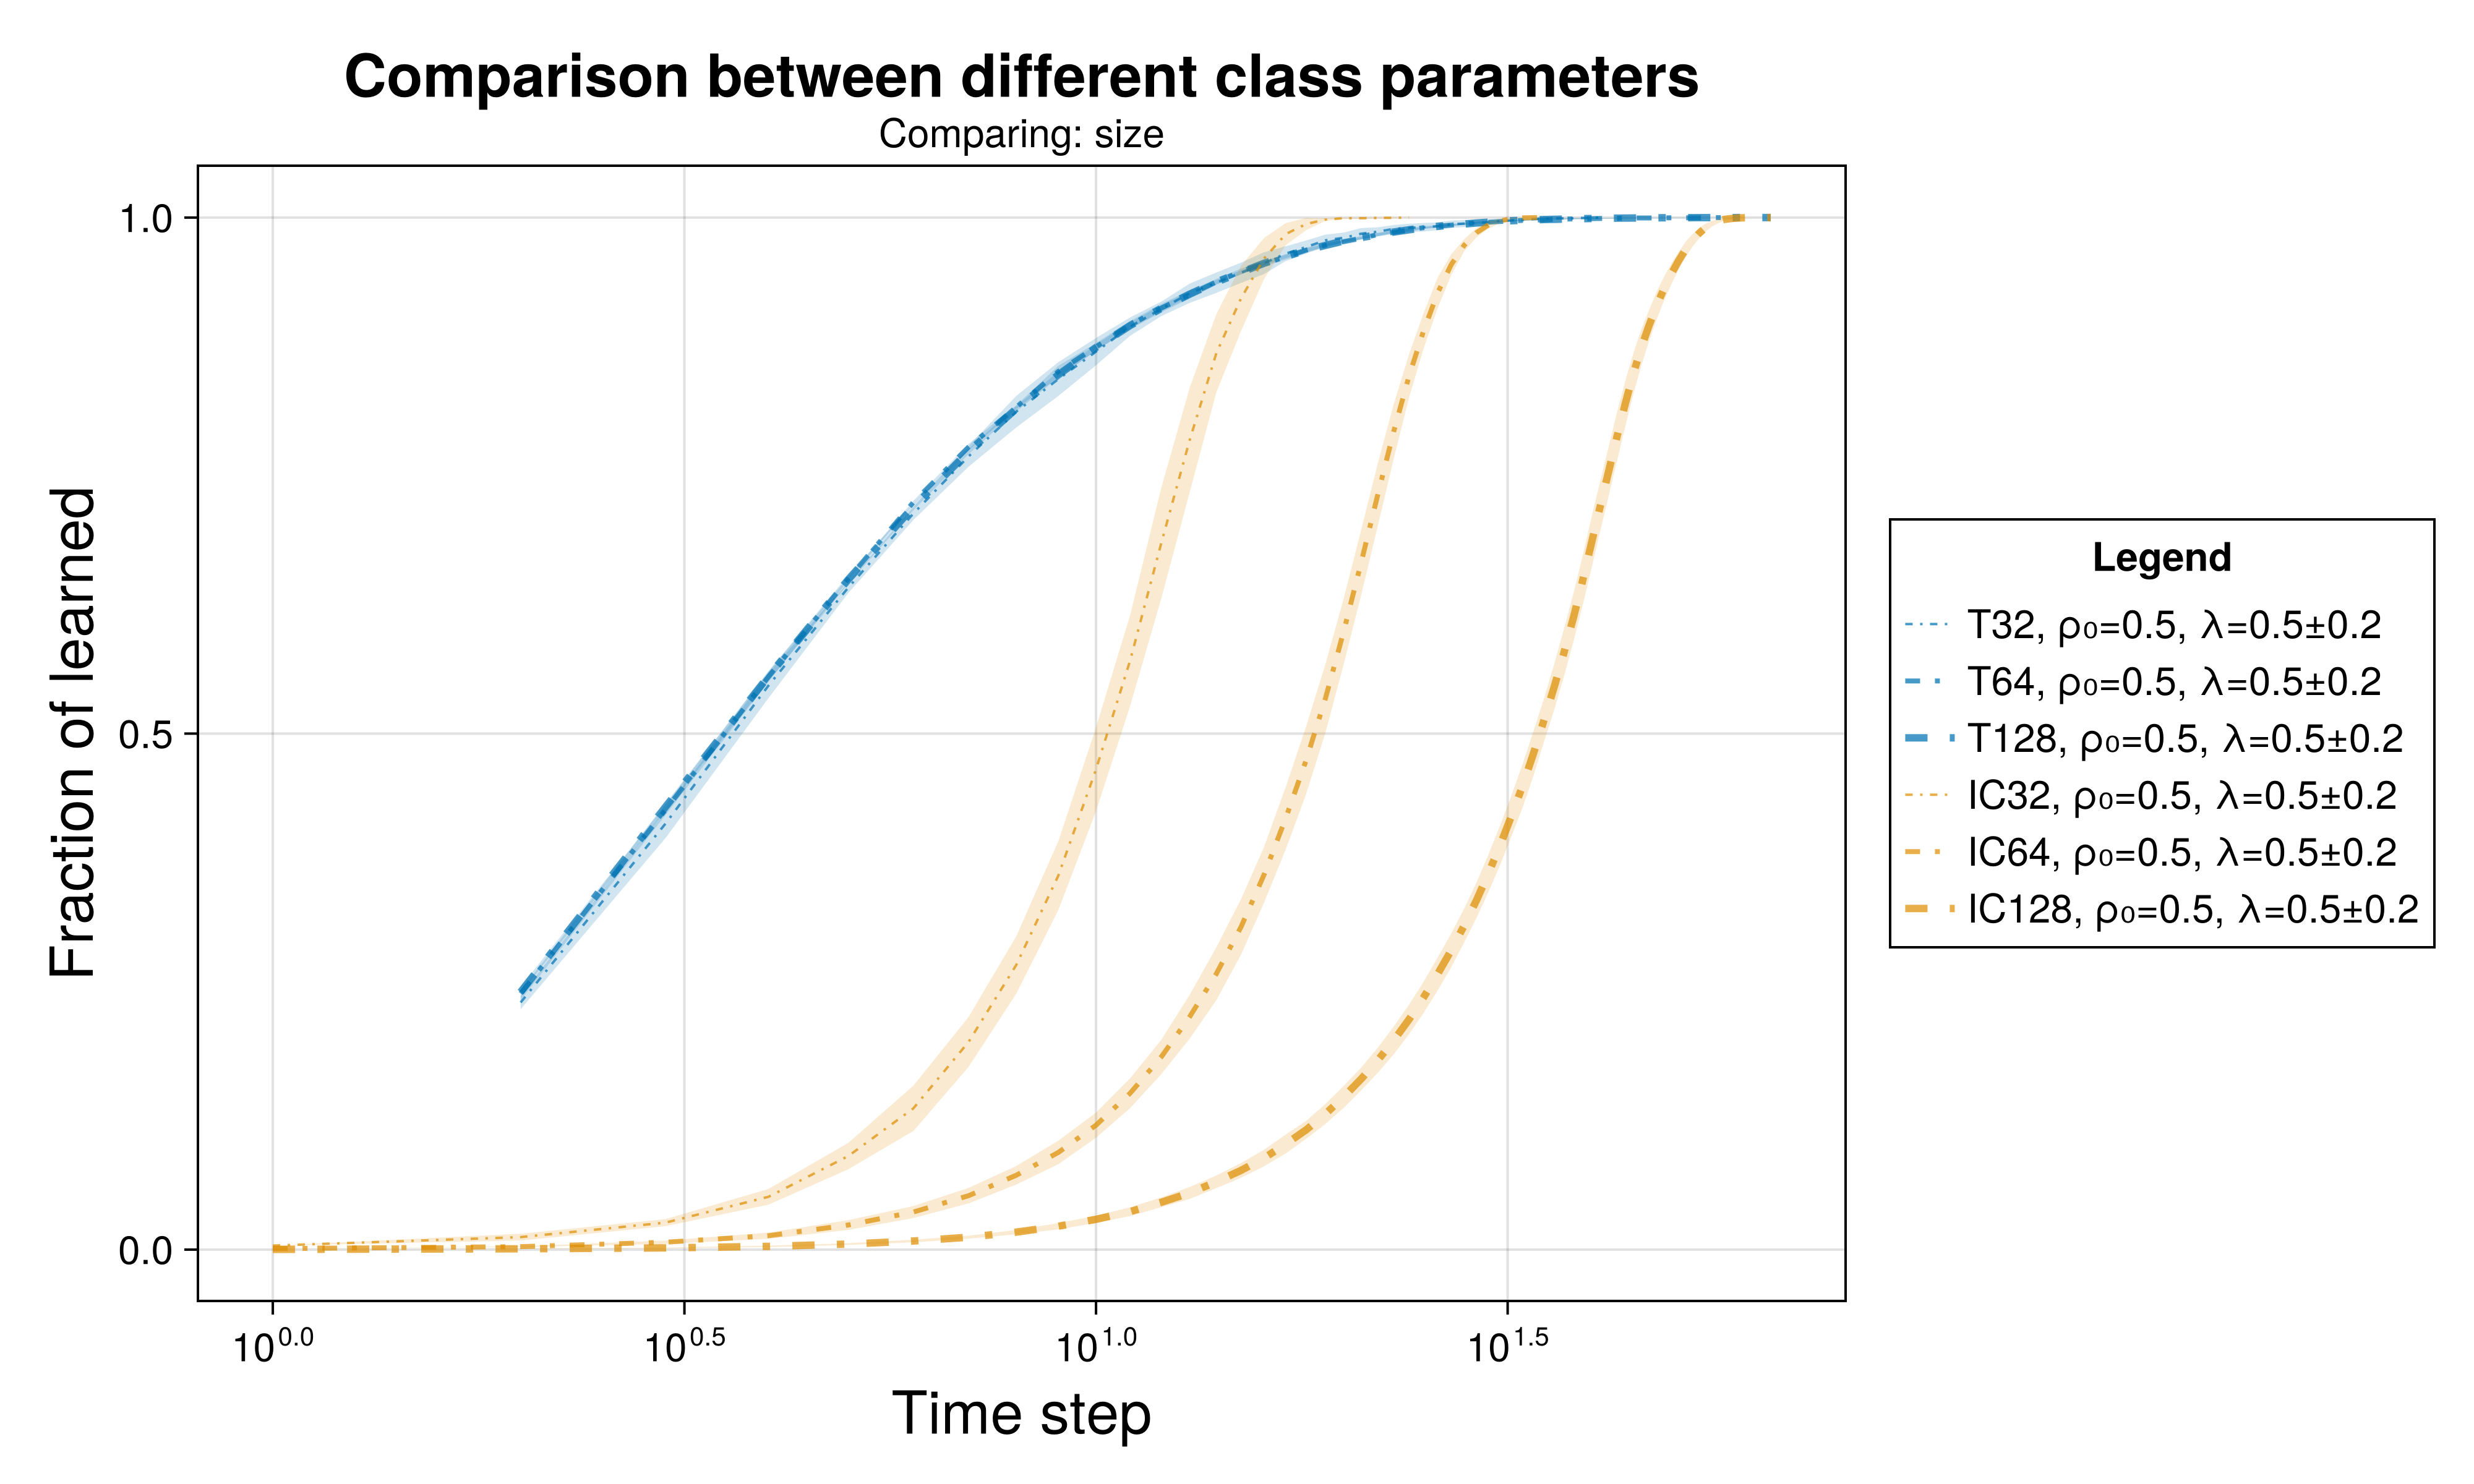
\includegraphics[width=0.49\textwidth]{figures/2D-BPCAIH-analysis/comparison plots/size.png}}
   \subfigure[$\rho_0$ comparison]{\label{fig:2DBPCAIH t-learned rho comparison}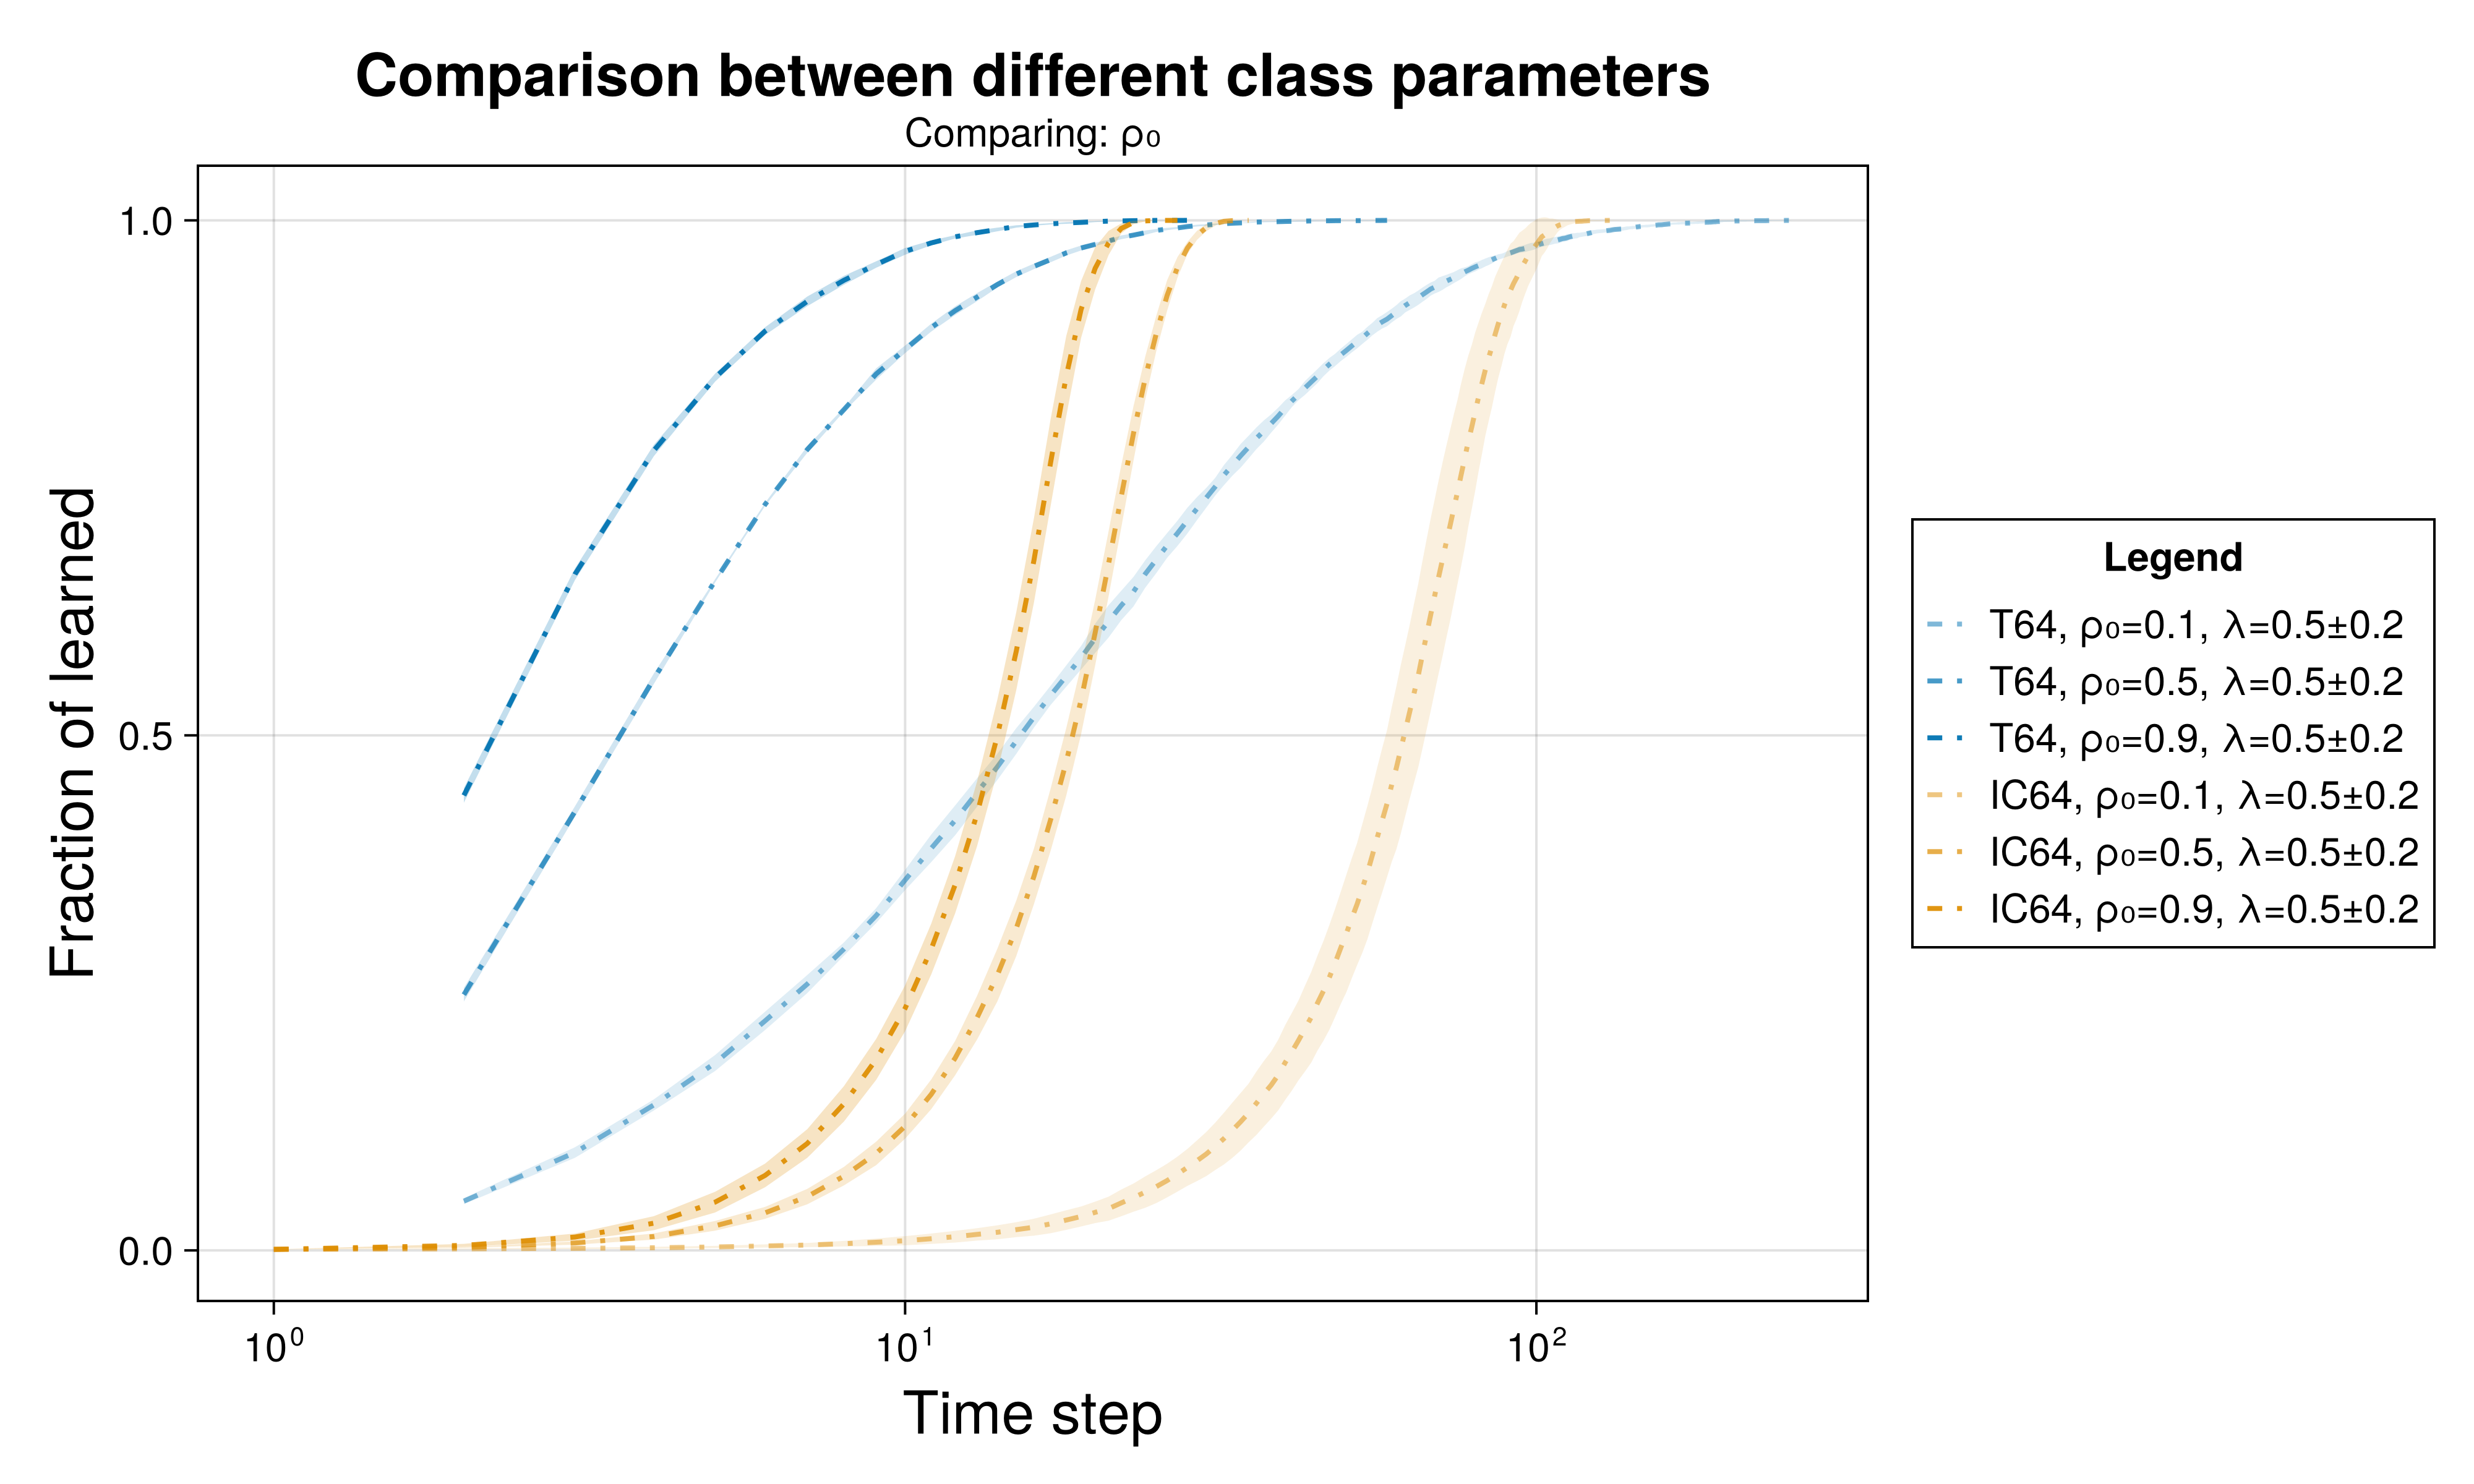
\includegraphics[width=0.49\textwidth]{figures/2D-BPCAIH-analysis/comparison plots/ρ₀.png}}
   \subfigure[$\delta\lambda$ comparison]{\label{fig:2DBPCAIH t-learned delta comparison}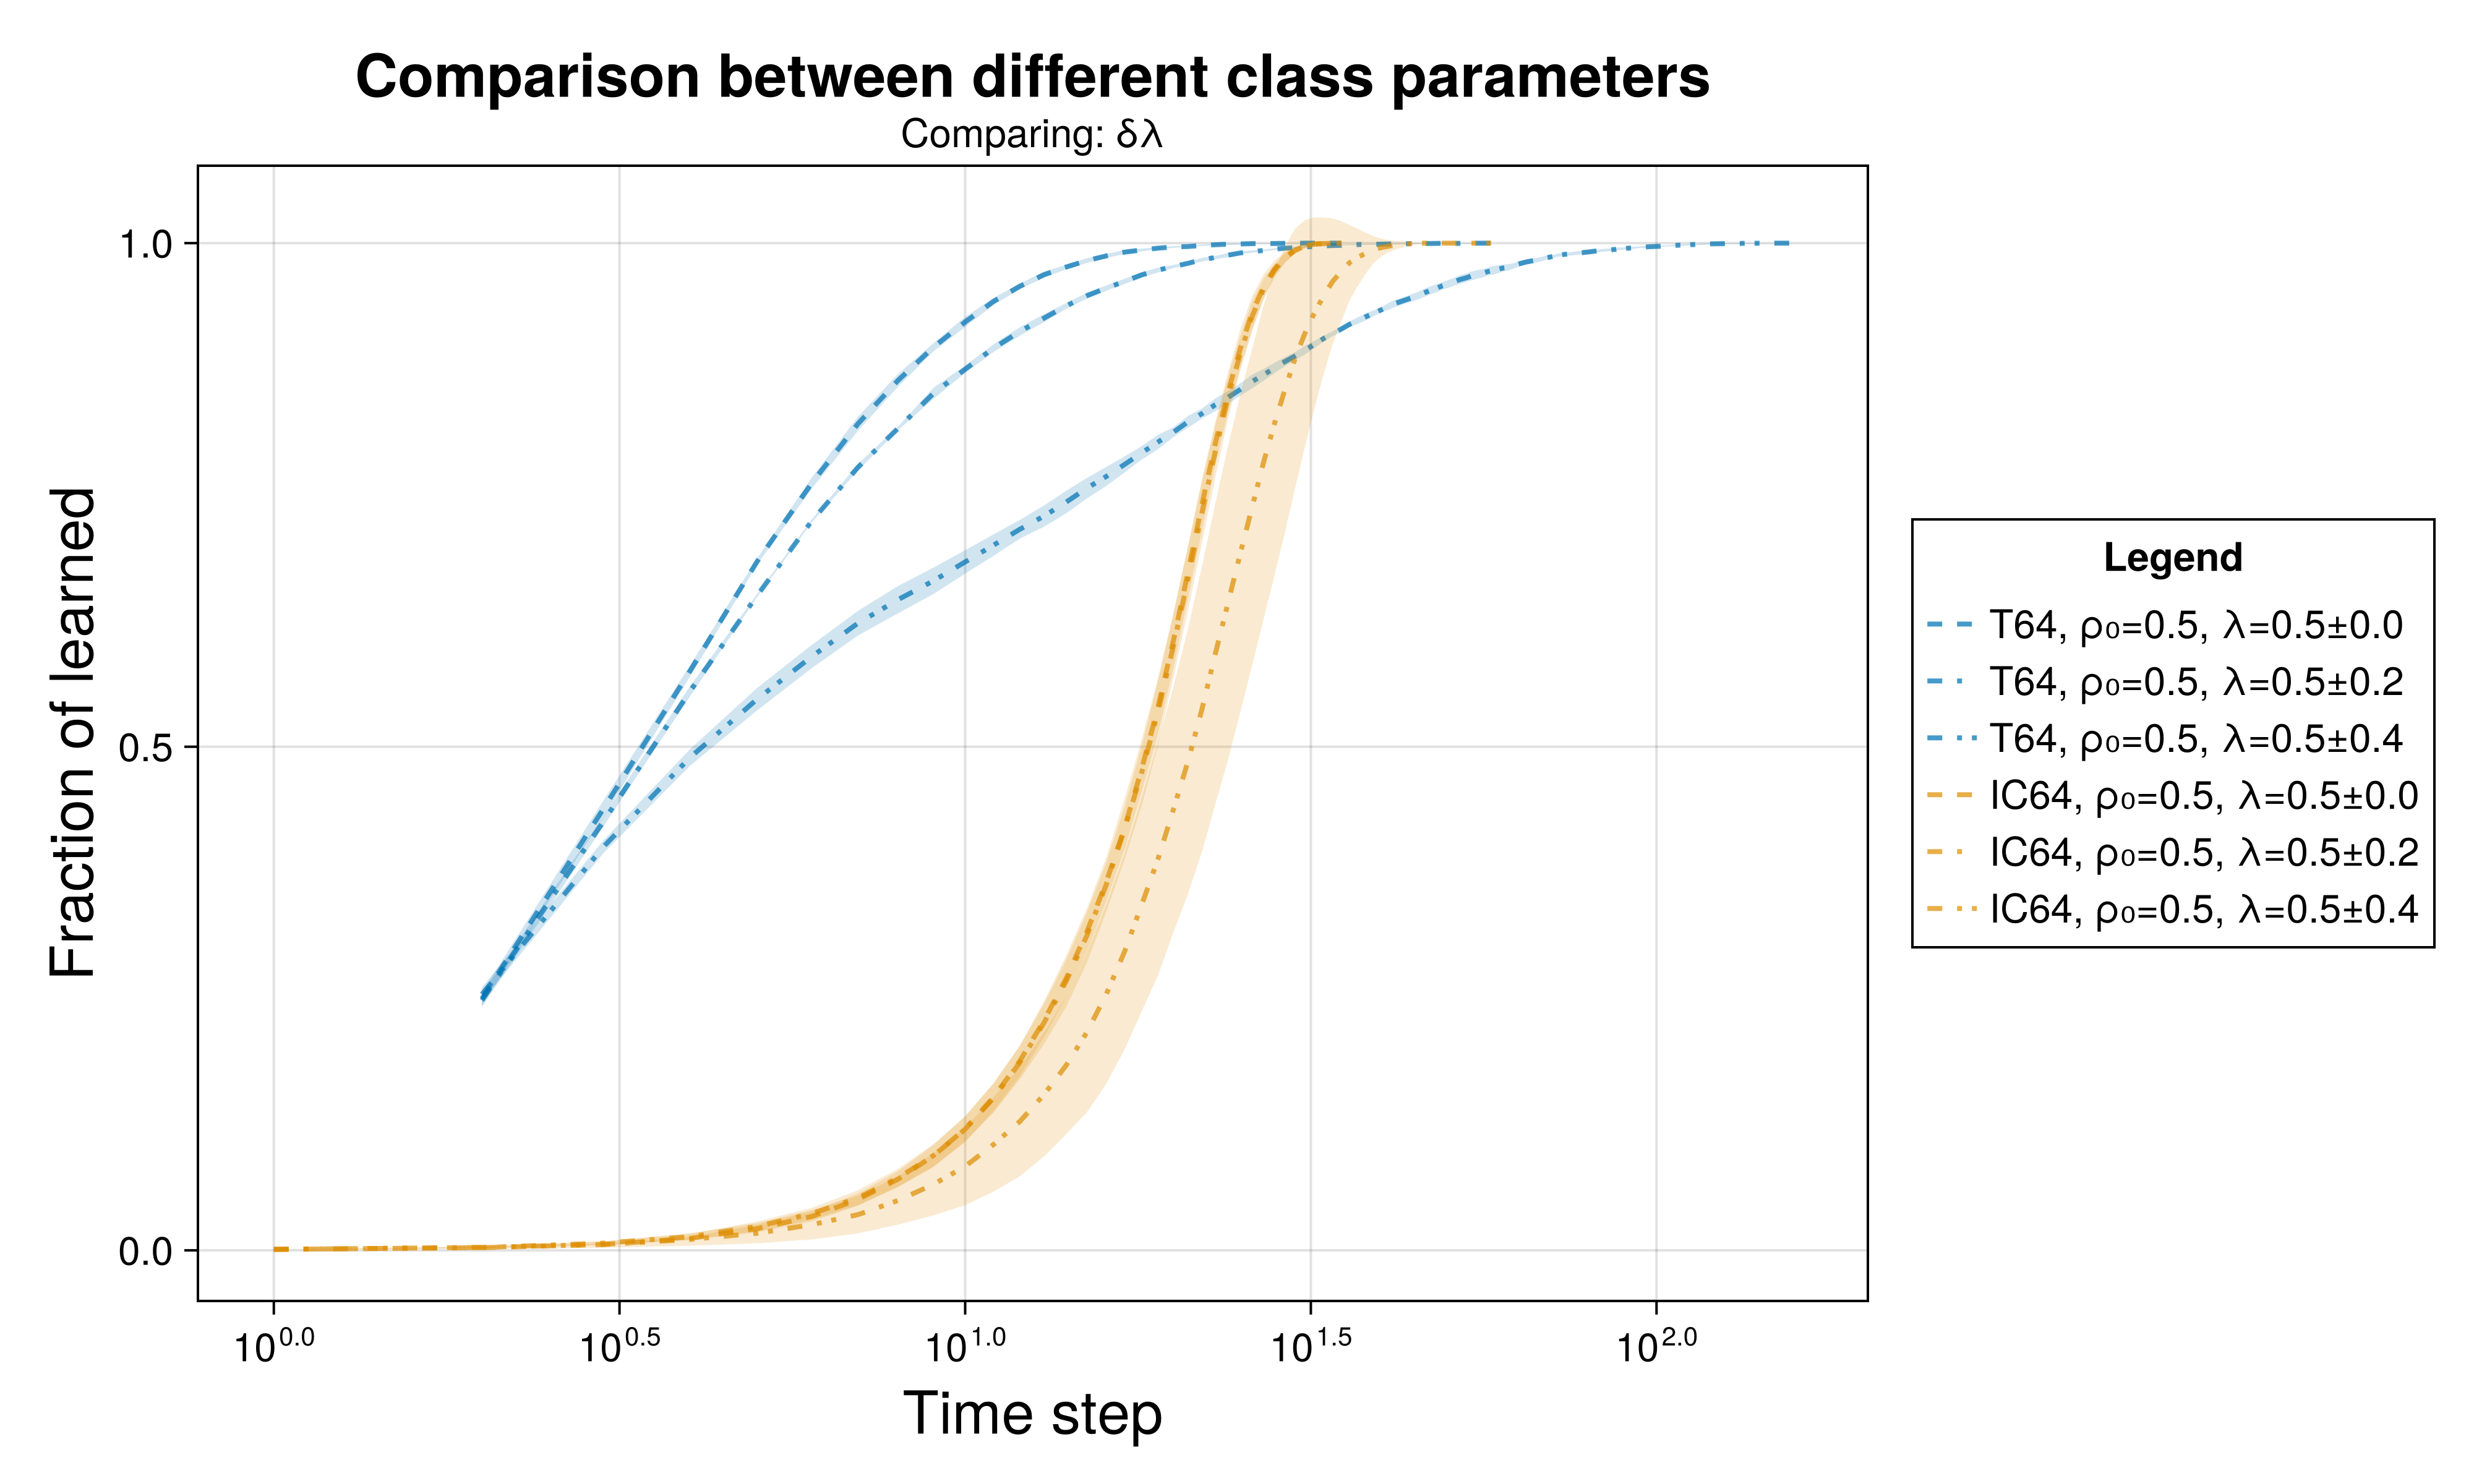
\includegraphics[width=0.49\textwidth]{figures/2D-BPCAIH-analysis/comparison plots/δλ.png}}
   \subfigure[SA comparison]{\label{fig:2DBPCAIH t-learned SA comparison}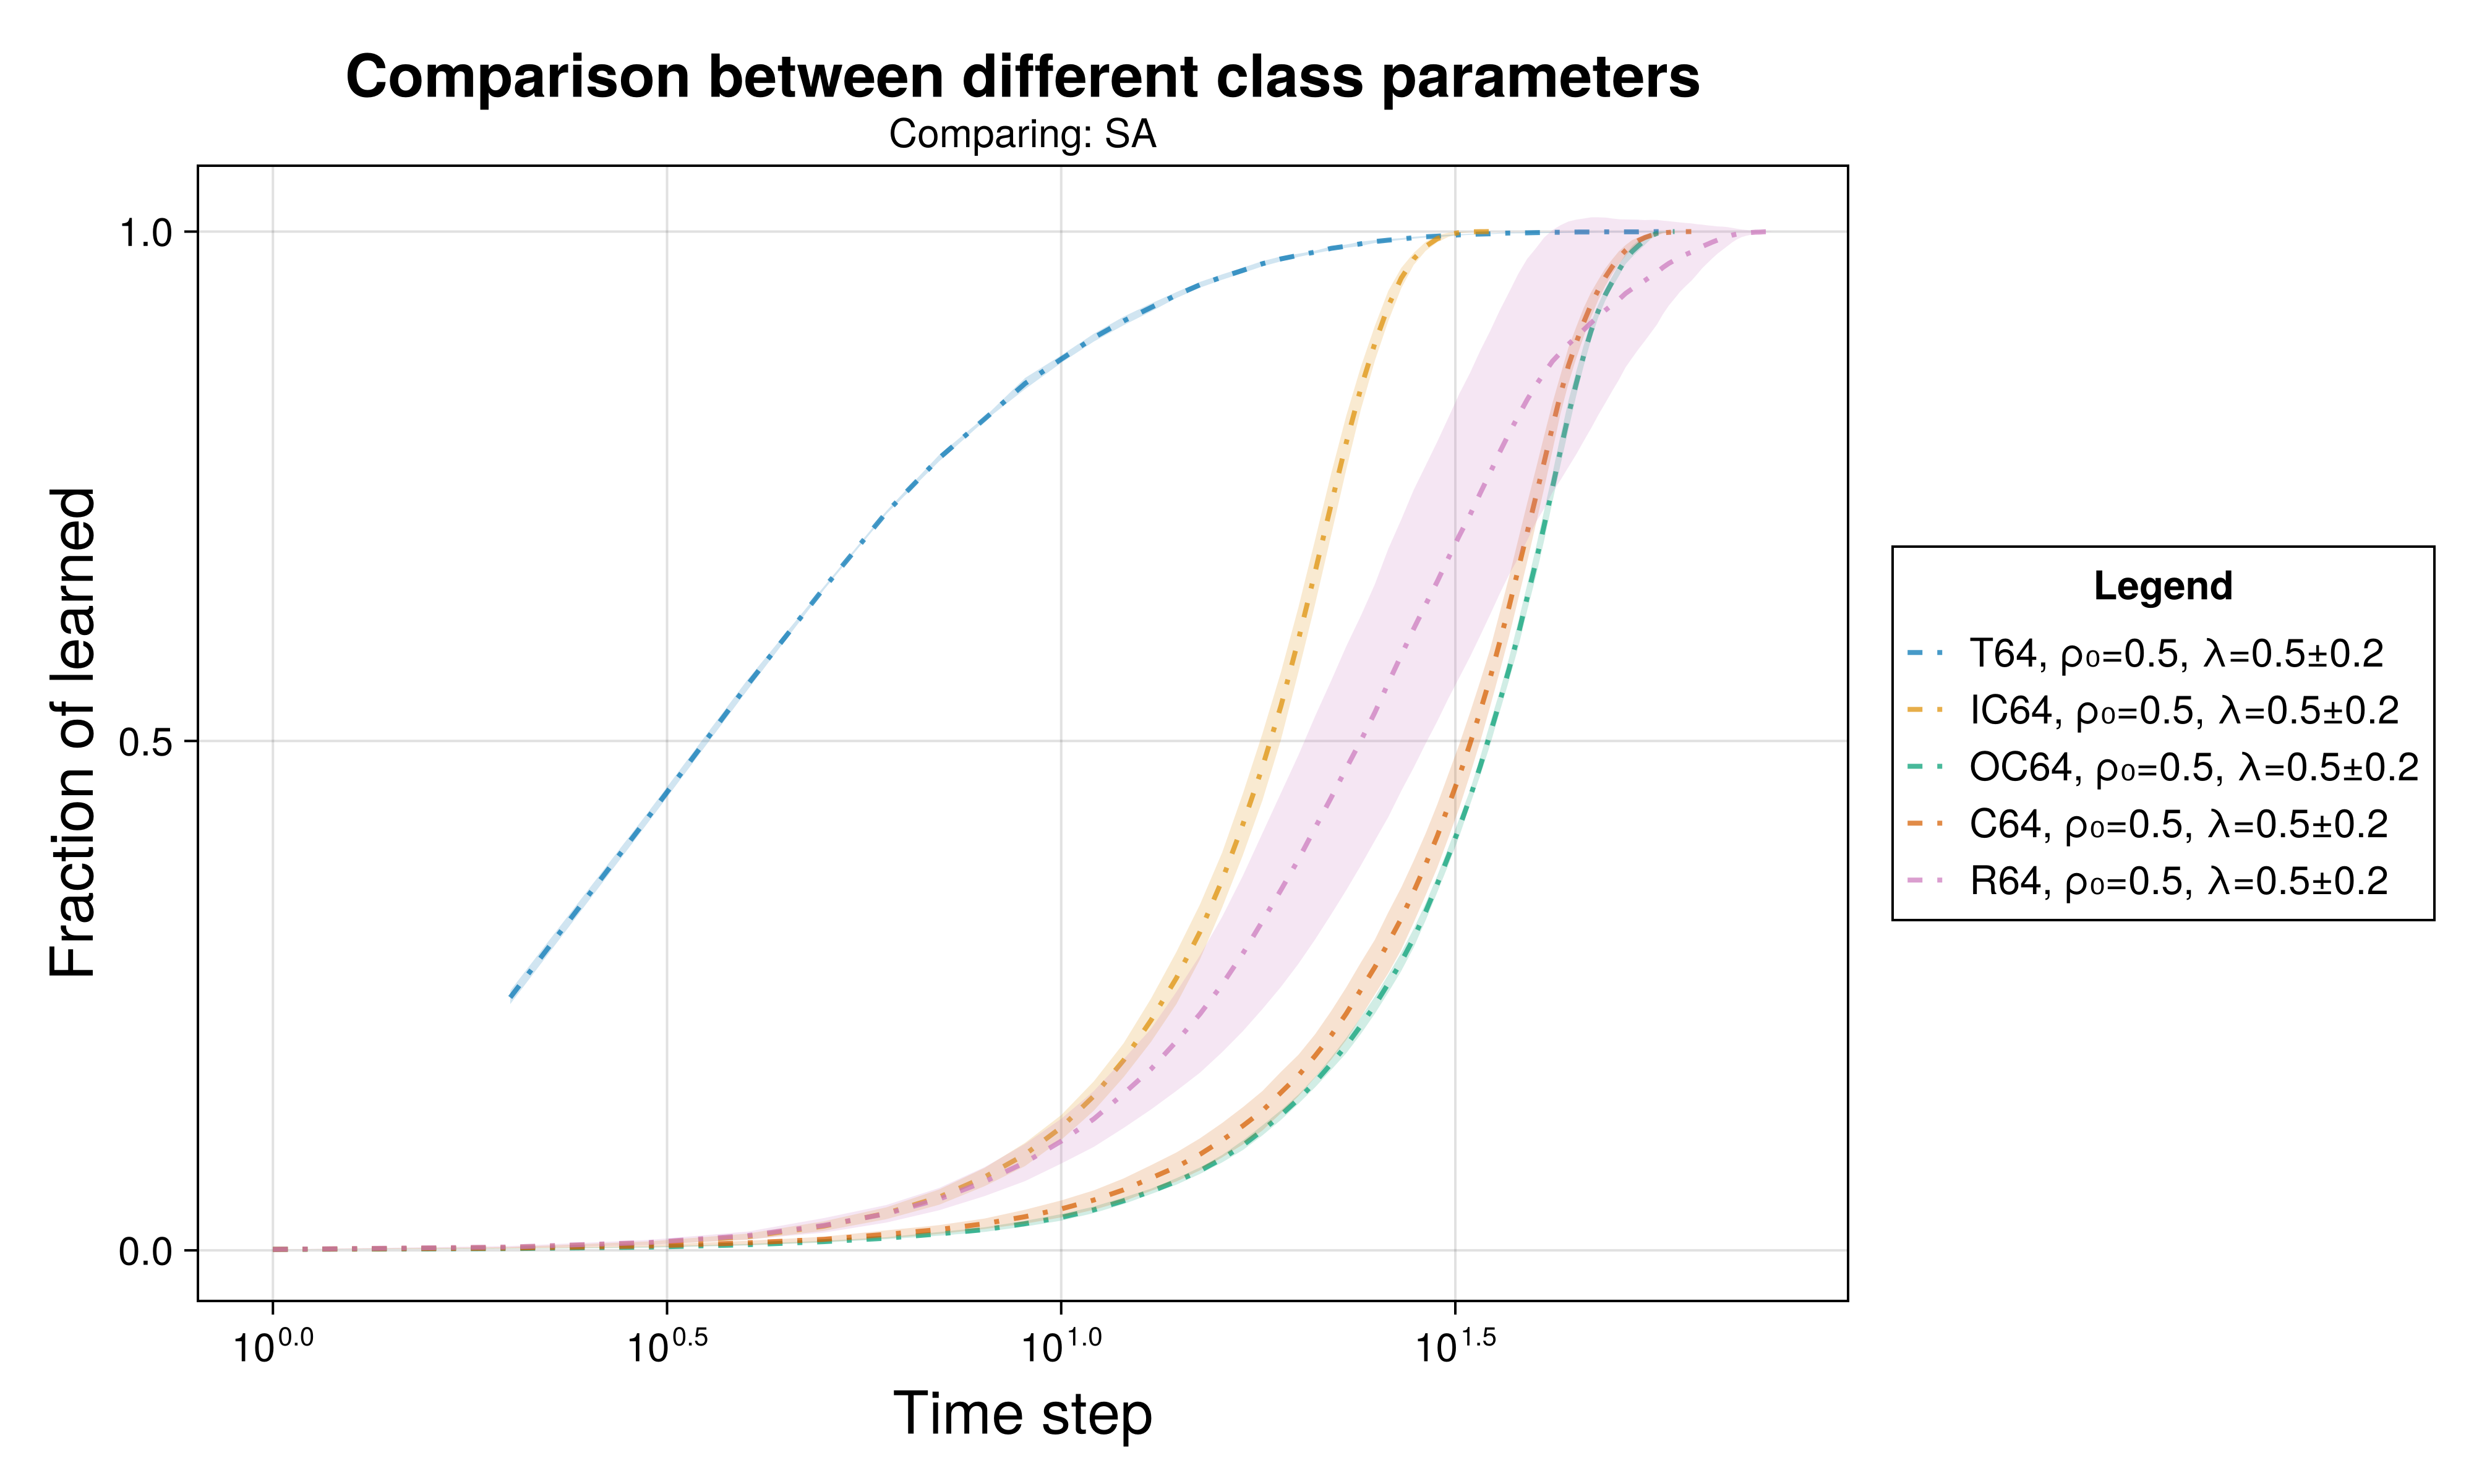
\includegraphics[width=0.49\textwidth]{figures/2D-BPCAIH-analysis/comparison plots/SA.png}}
   \caption{Comparison of time to learn $t_{max}$ and fraction of learned students for different representative classroom configurations. 
   Each SA corresponds to a different color, blue for traditional, yellow for inner corner, green for outer corner, orange for center, and pink for random. 
   Different values $\rho_0$ corresponds to varying alpha or transparency, where lower $\rho_0$ values are more transparent.
   Different values of $\delta\lambda$ corresponds to different line styles, where $\delta\lambda=0.0$ are represented by dashed lines, $\delta\lambda=0.2$ are represented by lines with alternating dots and dashes, $\delta\lambda=0.4$ are represented by two dots followed by a dash.
   Different classroom sizes $L$ corresponds to different line widths, where bigger classroom sizes correspond to thicker lines.
   The bands around each line show the standard deviation of the data over 5 trials.
   Higher fraction of learned indicates better performance.
   }
   \label{fig:2DBPCAIH t-learned comparisons}
\end{figure}

\newpage % new page after section class evolution

\section{Class learning rate $m$ vs positional learning factor $\rho_0$}\label{sec:BPCAIH m vs rho}

Figure~\ref{fig:2DBPCAIH m rho plot} shows that class learning rate becomes inconsistent with the positional learning factor $\rho_0$ in PI models when introducing heterogeneity. 
The inconsistency may be caused by sampling problem where the first 50\% of the data may not be just capturing the initial dynamics of the classroom, which should be the only basis of the class learning rate $m$.
With heterogeneity, PI models no longer show trends in learning rate $m$ as a function of positional learning factor $\rho_0$.

The traditional instruction model shows a similar trend in learning rate $m$ as with time to learn $t_{max}$ where homogenous classrooms perform better then heterogenous classrooms.
This might be explained by the spatiotemporal dynamics of traditional learning models where the fast learning students learn first and the slow learning students learn last, as discussed in Section \ref{sec:BPCAIH effects on classroom evolution} and shown in Figure~\ref{fig:2DBPCAIH sample class evolution trad low rho high delta}.

Moving forward, we will only focus on the time to learn $t_{max}$ as a metric for performance.

\begin{figure}[htbp!]
   \centering
   \subfigure[Center $L=32$]{\label{fig:BPCAIH m plot C32}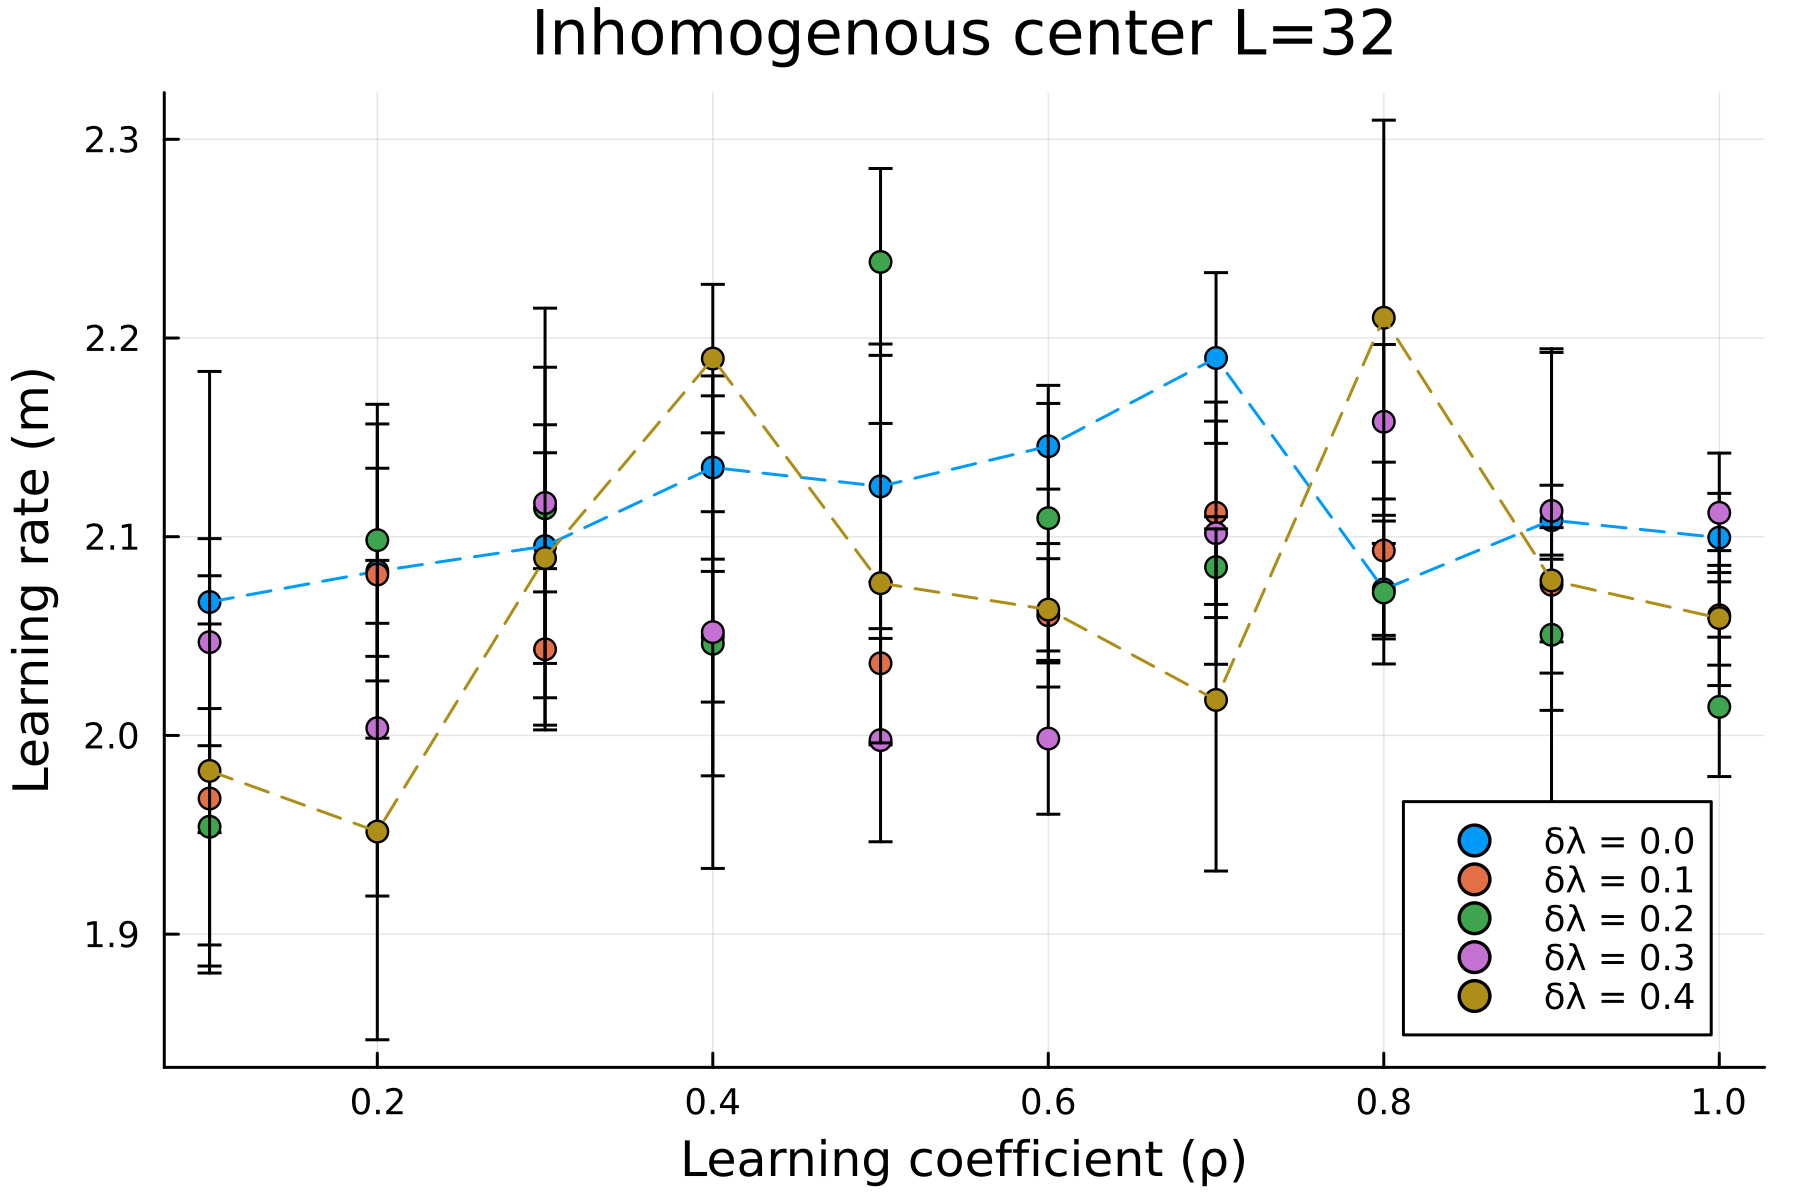
\includegraphics[width=0.40\textwidth]{figures/2D-BPCAIH-analysis/m-plots/m-center-32.png}}
   \subfigure[Outer corner $L=48$]{\label{fig:BPCAIH m plot O48}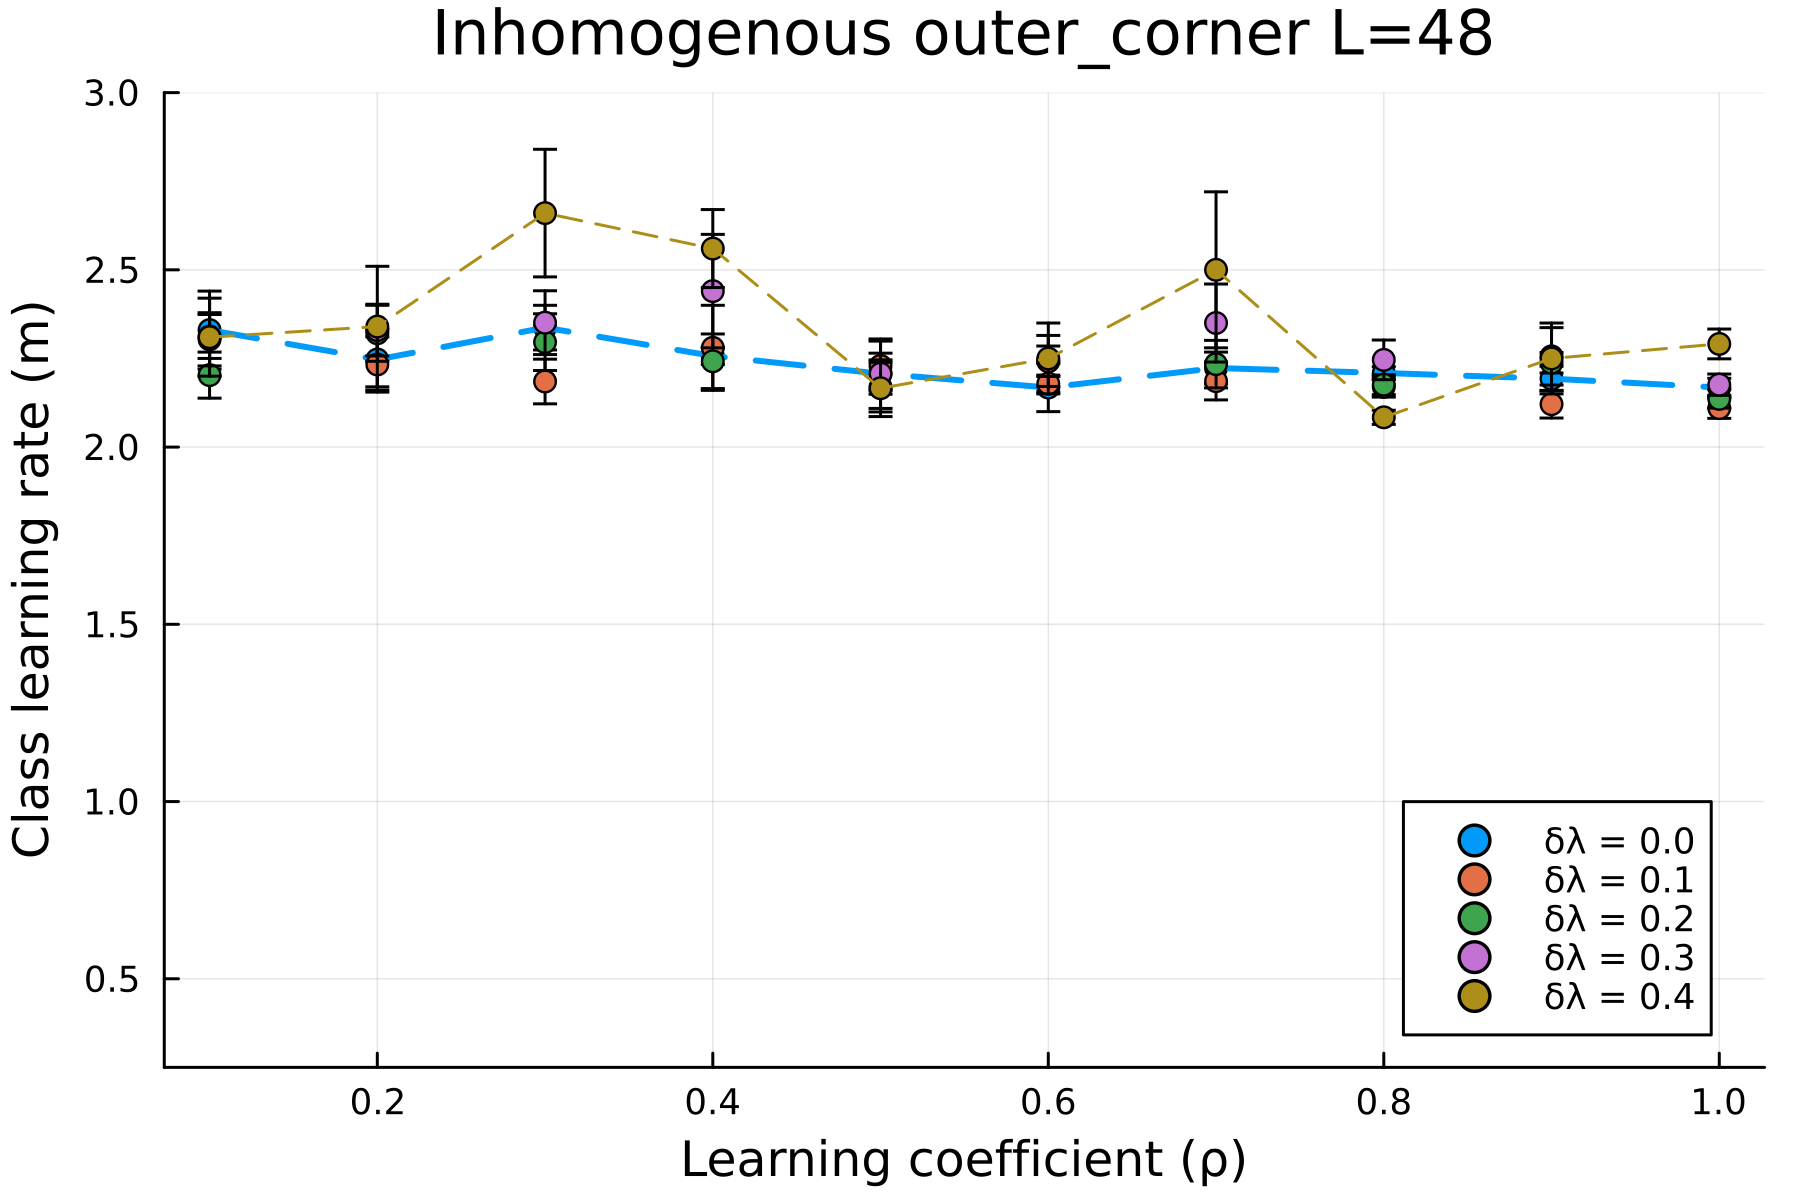
\includegraphics[width=0.40\textwidth]{figures/2D-BPCAIH-analysis/m-plots/m-outer_corner-48.png}}
   \subfigure[Inner corner $L=64$]{\label{fig:BPCAIH m plot I64}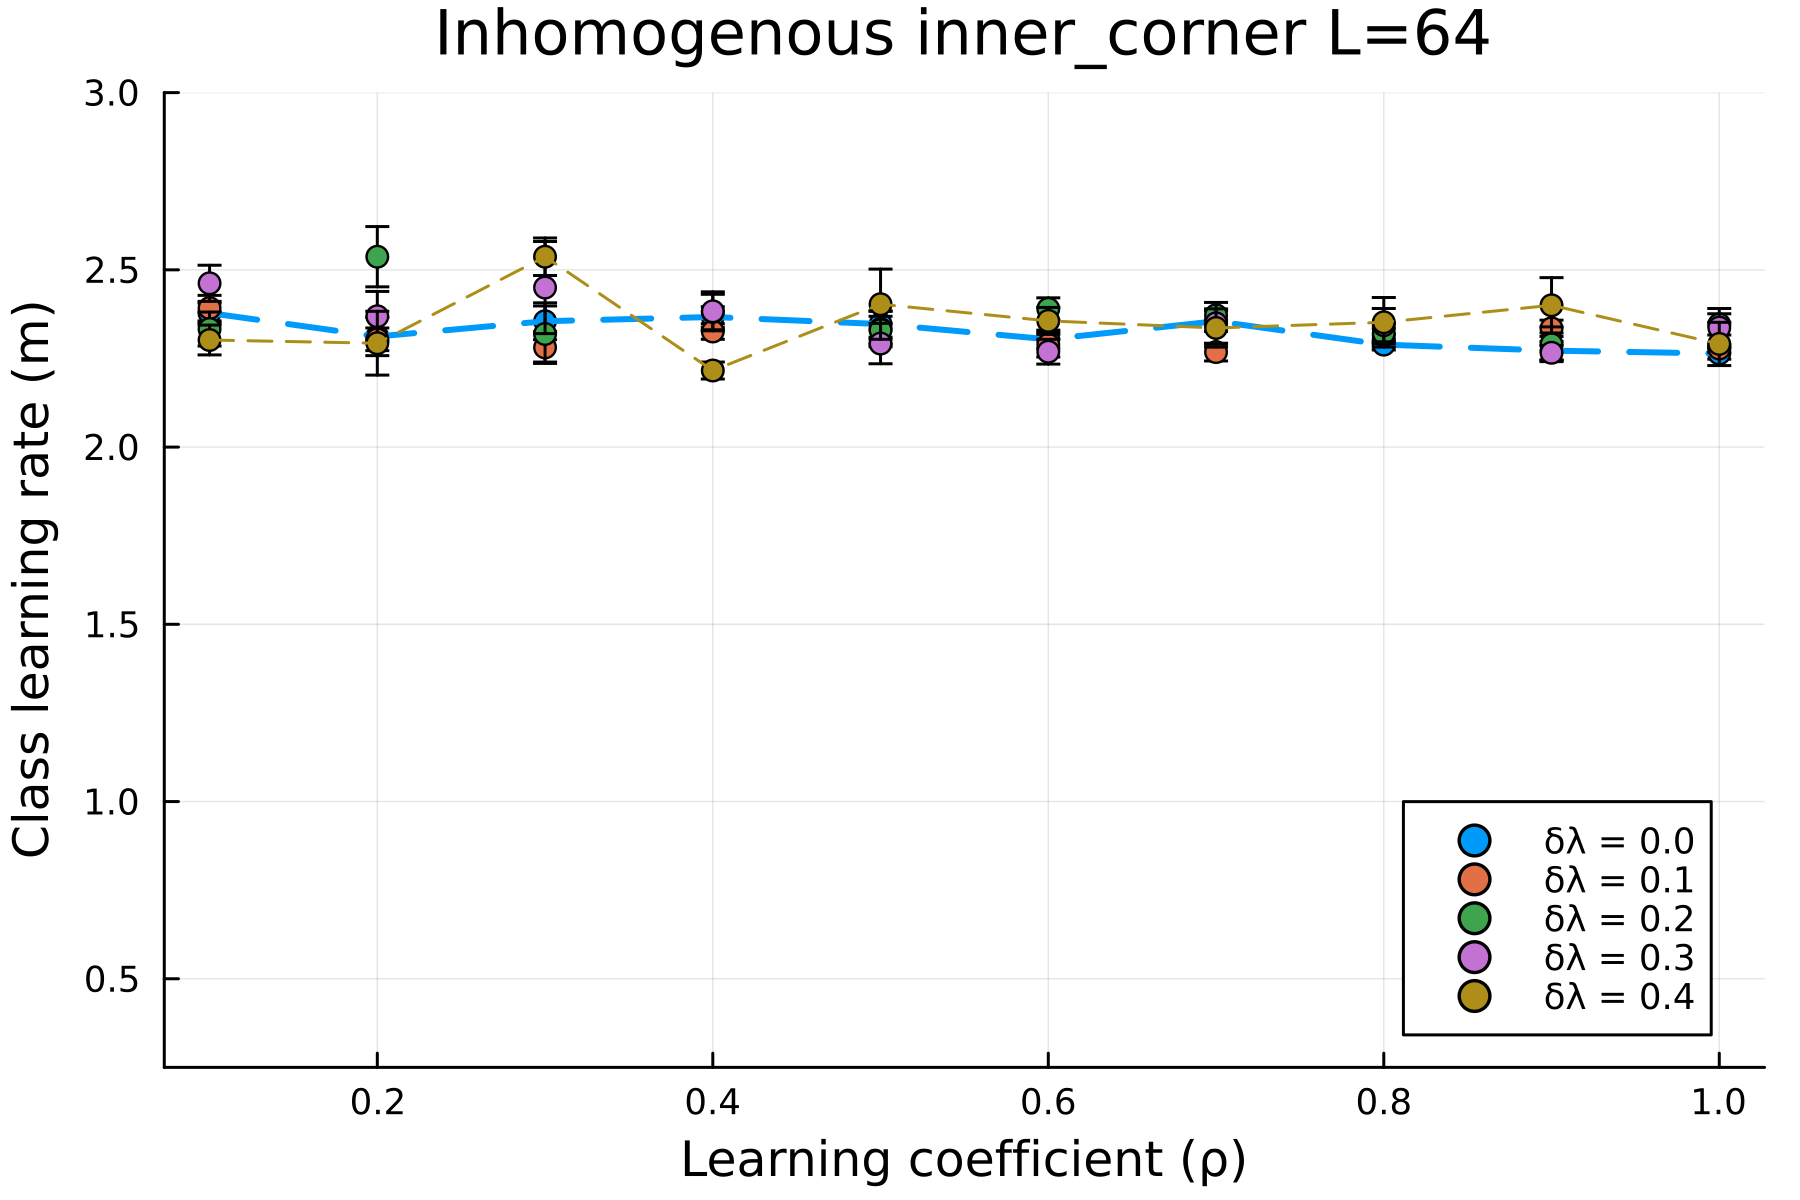
\includegraphics[width=0.40\textwidth]{figures/2D-BPCAIH-analysis/m-plots/m-inner_corner-64.png}}
   \subfigure[Random $L=96$]{\label{fig:BPCAIH m plot R96}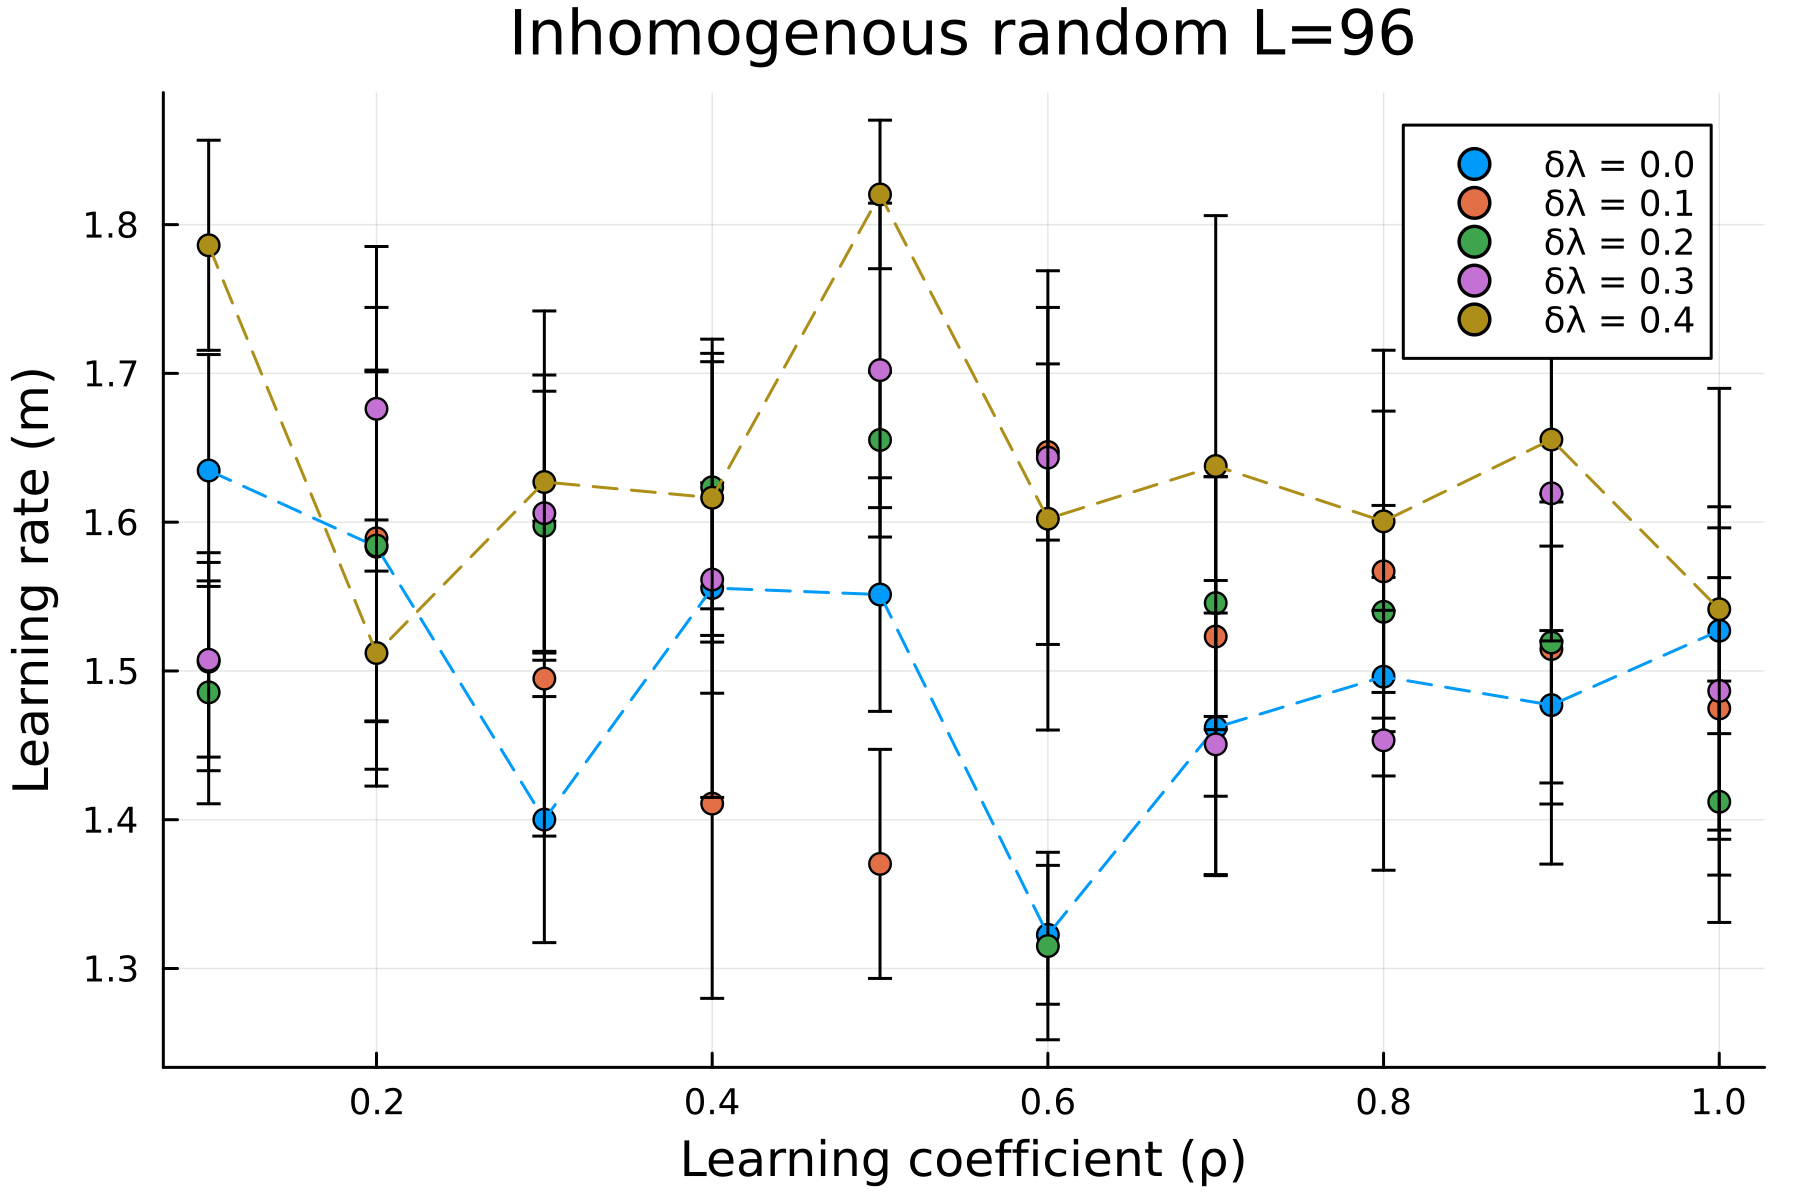
\includegraphics[width=0.40\textwidth]{figures/2D-BPCAIH-analysis/m-plots/m-random-96.png}}
   \subfigure[Traditional $L=128$]{\label{fig:BPCAIH m plot T128}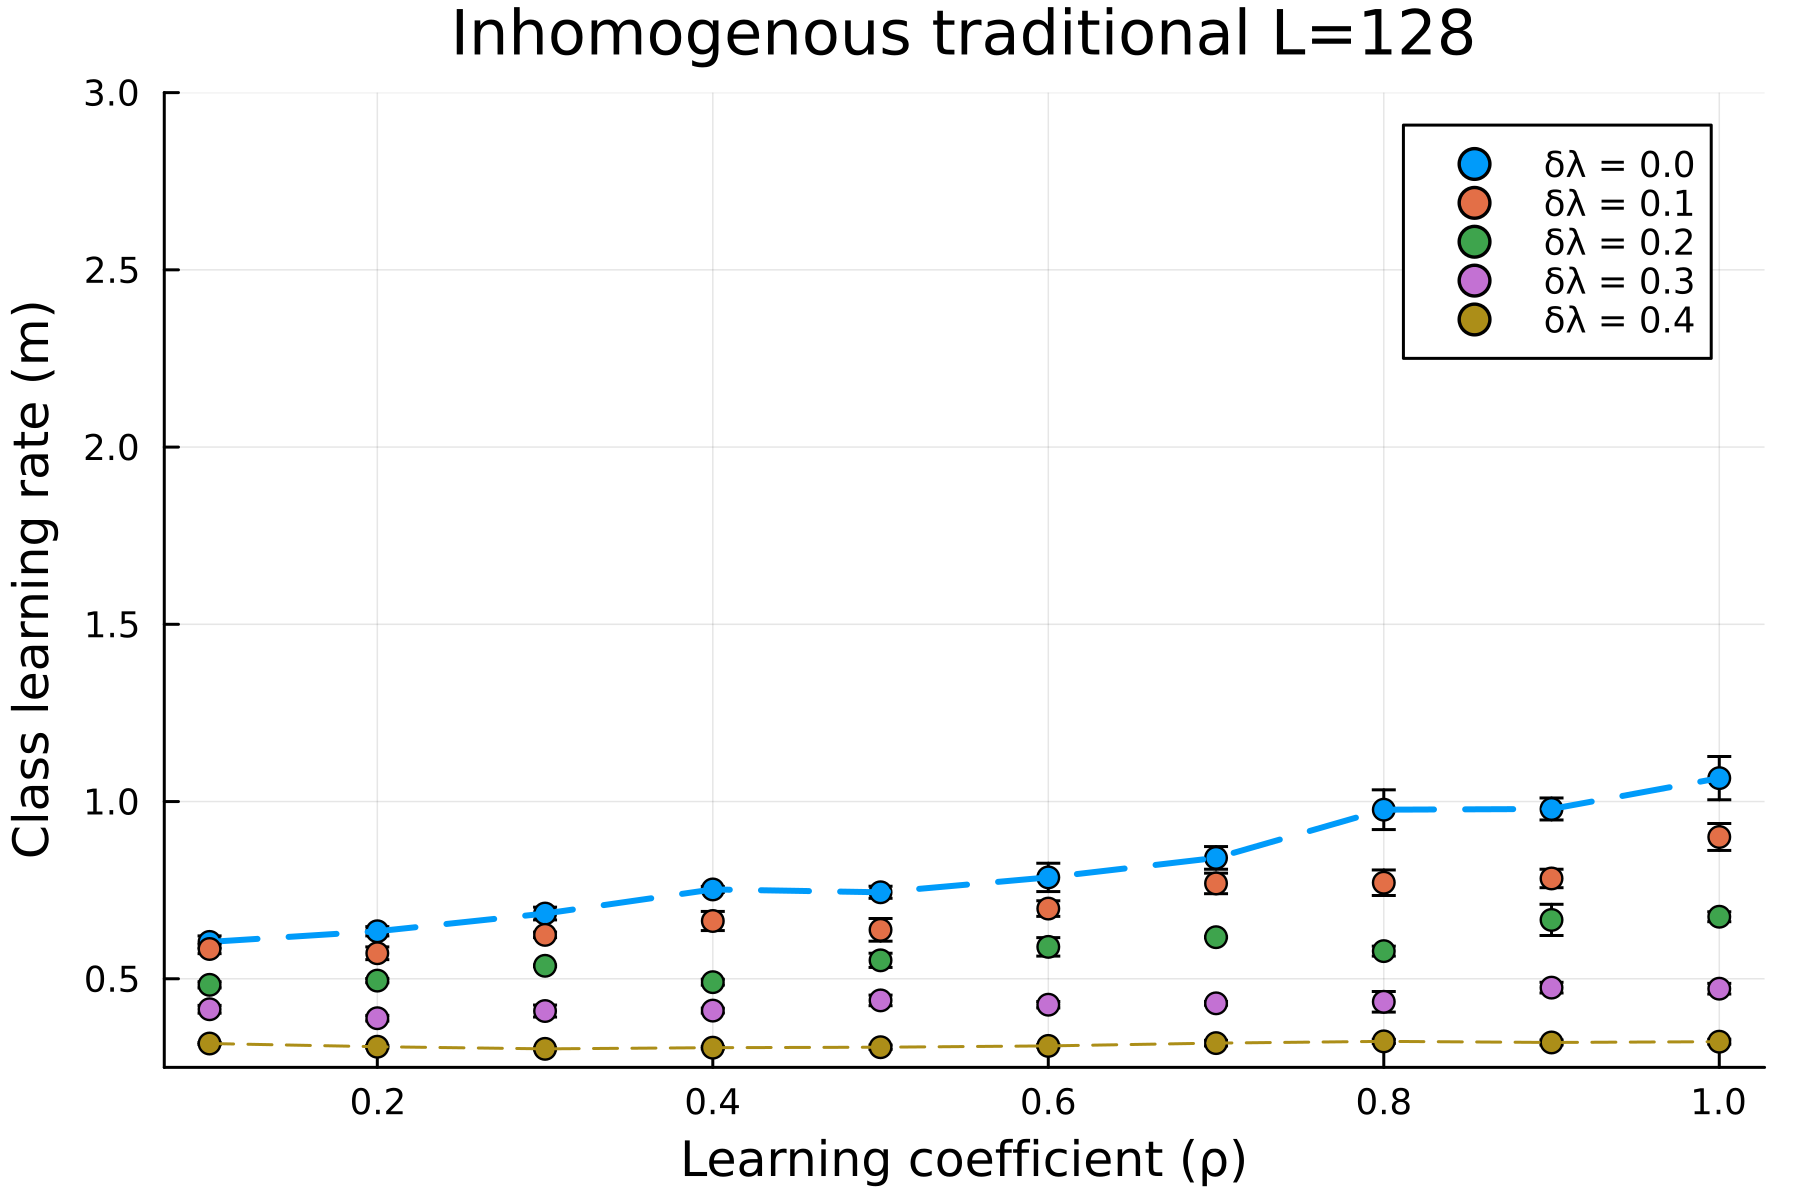
\includegraphics[width=0.40\textwidth]{figures/2D-BPCAIH-analysis/m-plots/m-traditional-128.png}}
   
   \caption{Representative plots for class learning rate $m$ as a function of positional learning coefficient $\rho_0$.
   Each subplot represent a different SA and classroom size $L$.
   In each plot, the circles represent the data points, color represents a different value of $\delta\lambda \in \lbrace 0.0, 0.1, 0.2, 0.3, 0.4 \rbrace$, dashed lines connect the data points for $\delta\lambda \in \lbrace 0.0, 0.4 \rbrace$.
   Higher class learning rate m values indicate better performance.
   }
   \label{fig:2DBPCAIH m rho plot}
\end{figure}

\newpage % new page after section m vs rho

\section{Time to learn $t_{max}$ vs positional learning factor $\rho_0$}\label{sec:BPCAIH t vs rho}
Figure~\ref{fig:2DBPCAIH t-rho plot} shows the time to learn $t_{max}$ is directly affected by the level of heterogeneity $\delta\lambda$. 
This means that the heterogeneity $\delta\lambda$ has a significant effect on the time to learn $t_{max}$, with lower values of $\delta\lambda$ leading to lower time to learn $t_{max}$ for all values of $\rho_0$. 
We also notice that the traditional model is more affected by classroom heterogeneity comapred to PI models.

When aggregating the different results for each class size $L$, as shown in Figure~\ref{fig:2DBPCAIH t-rho ribbon plot}, it affirms our previous findings that PI models are better for smaller clases and lower values of $\rho_0$.
This stays consistent when comparing the performance of a similar classroom size $L$ and heterogeneity $\delta\lambda$ using the traditional model.
However, the comparison is not as clear when comparing between different levels of heterogeneity $\delta\lambda$.
When $L\geq64$, the PI models can perform better than the traditional model depending on the heterogeneity $\delta\lambda$, even with the same positional learning factor $\rho_0$.

\begin{figure}[htbp!]
   \centering
   \subfigure[Outer corner $L=48$]{\label{fig:2DBPCAIH t-rho plot OC48}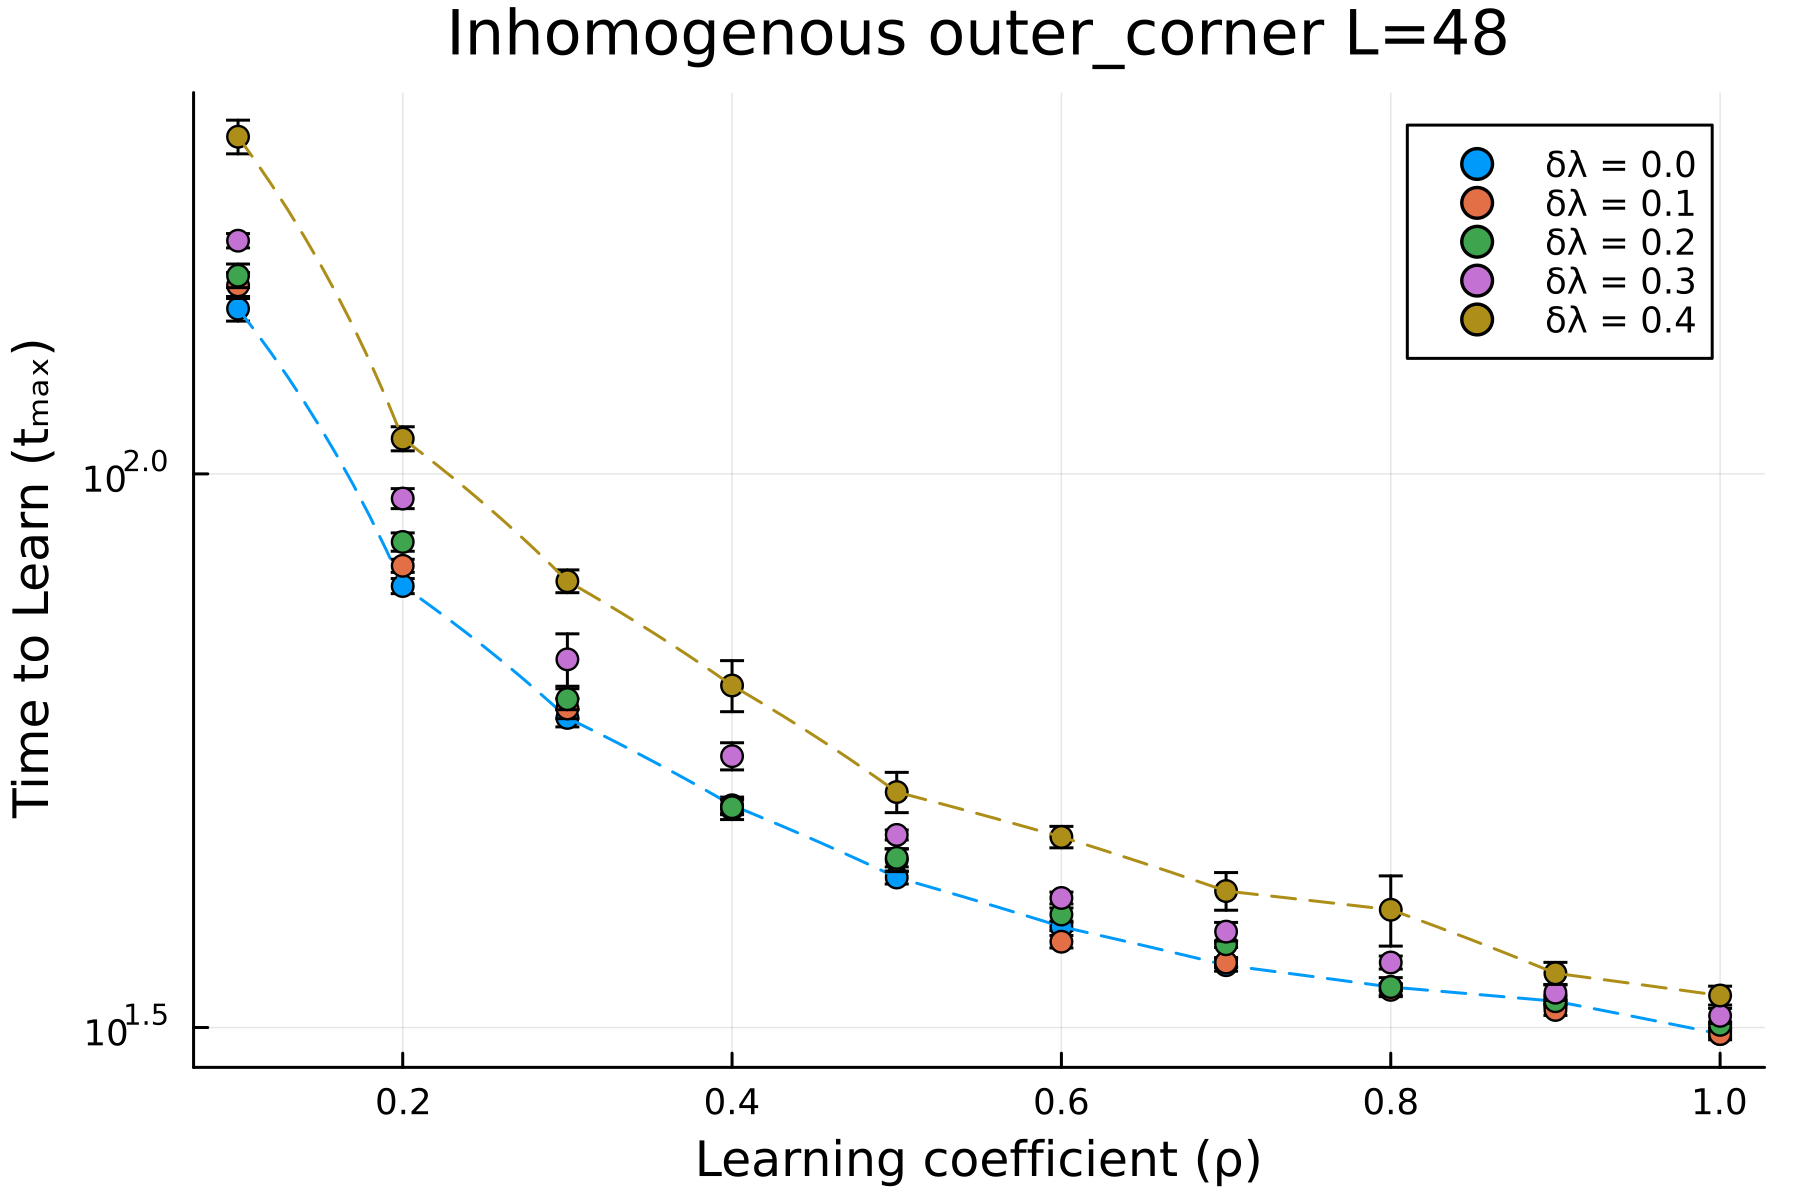
\includegraphics[width=0.49\textwidth]{figures/2D-BPCAIH-analysis/t-plots/t-outer_corner-48.png}}
   \subfigure[Outer corner $L=96$]{\label{fig:2DBPCAIH t-rho plot OC96}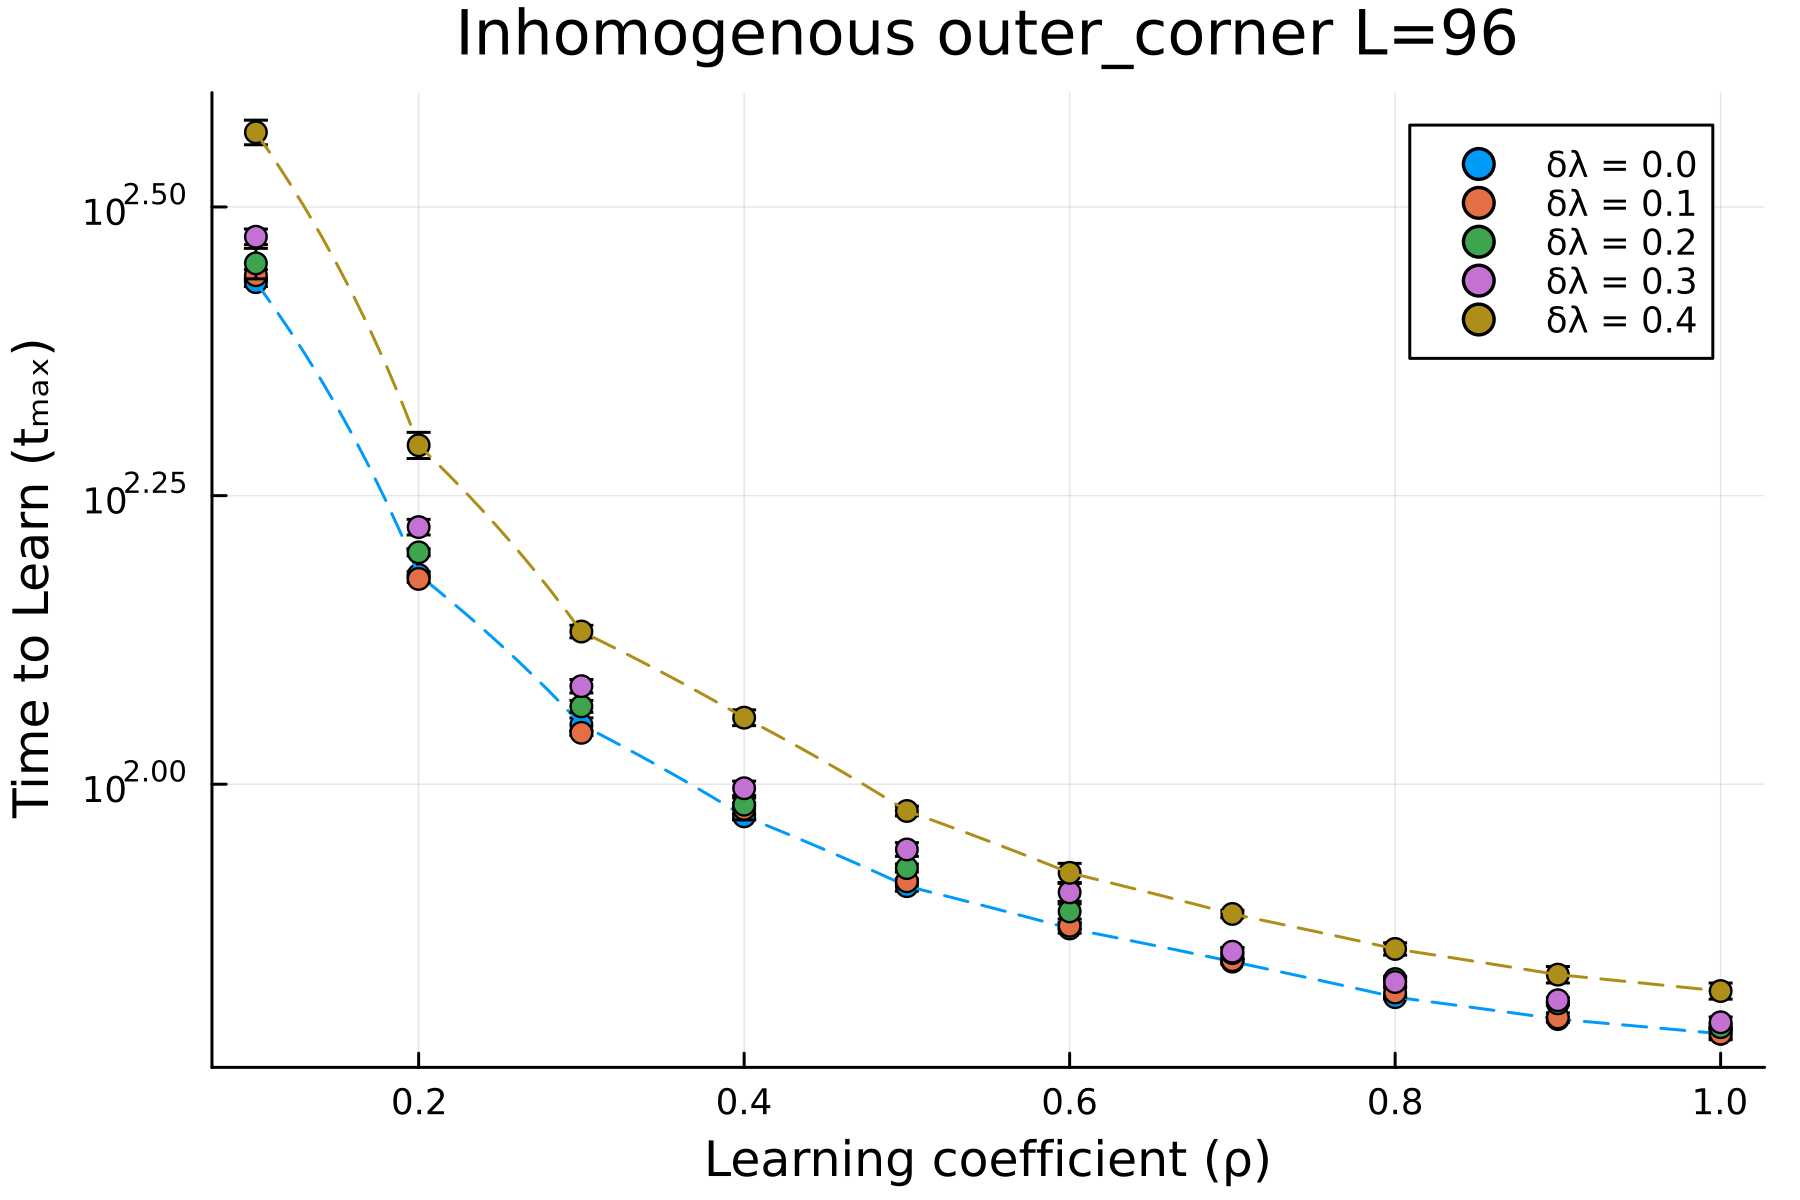
\includegraphics[width=0.49\textwidth]{figures/2D-BPCAIH-analysis/t-plots/t-outer_corner-96.png}}
   \subfigure[Inner corner $L=48$]{\label{fig:2DBPCAIH t-rho plot IC48}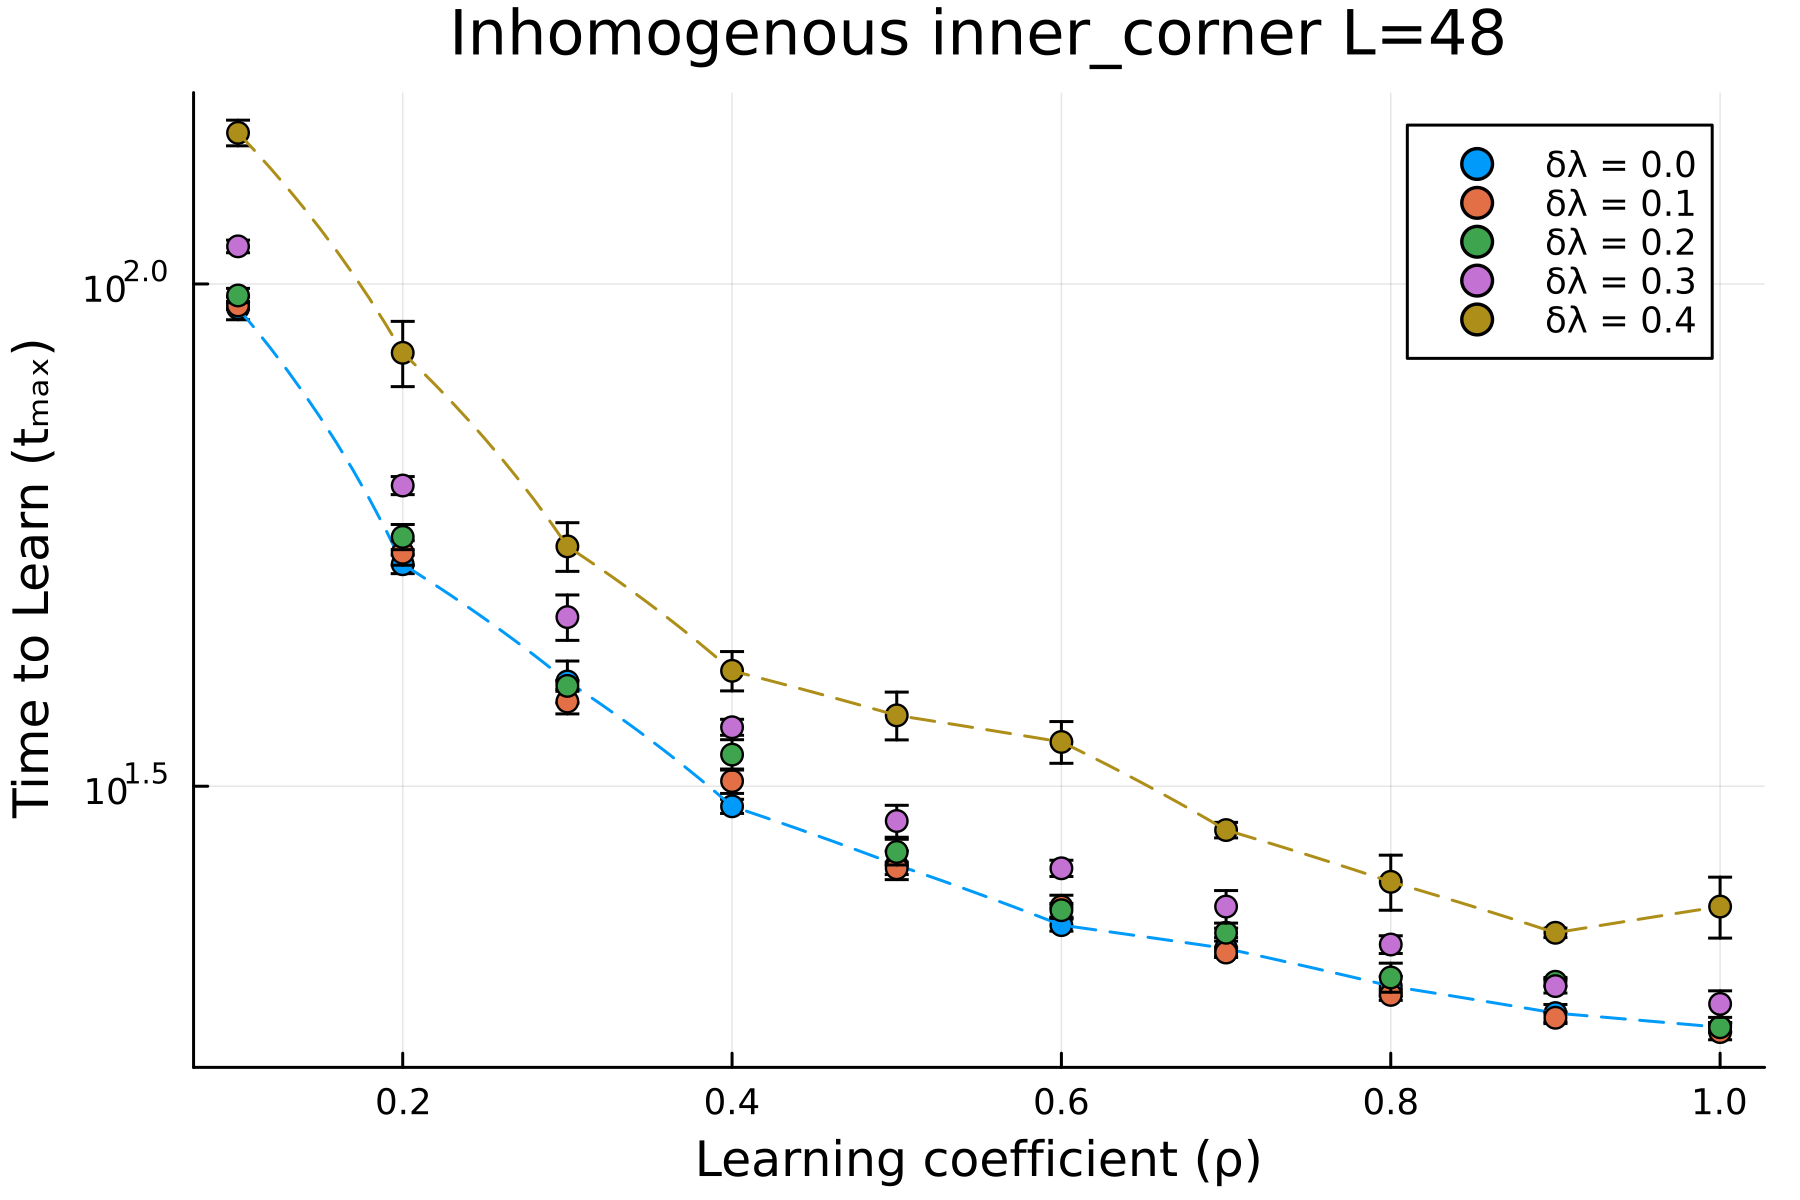
\includegraphics[width=0.49\textwidth]{figures/2D-BPCAIH-analysis/t-plots/t-inner_corner-48.png}}
   \subfigure[Inner corner $L=96$]{\label{fig:2DBPCAIH t-rho plot IC96}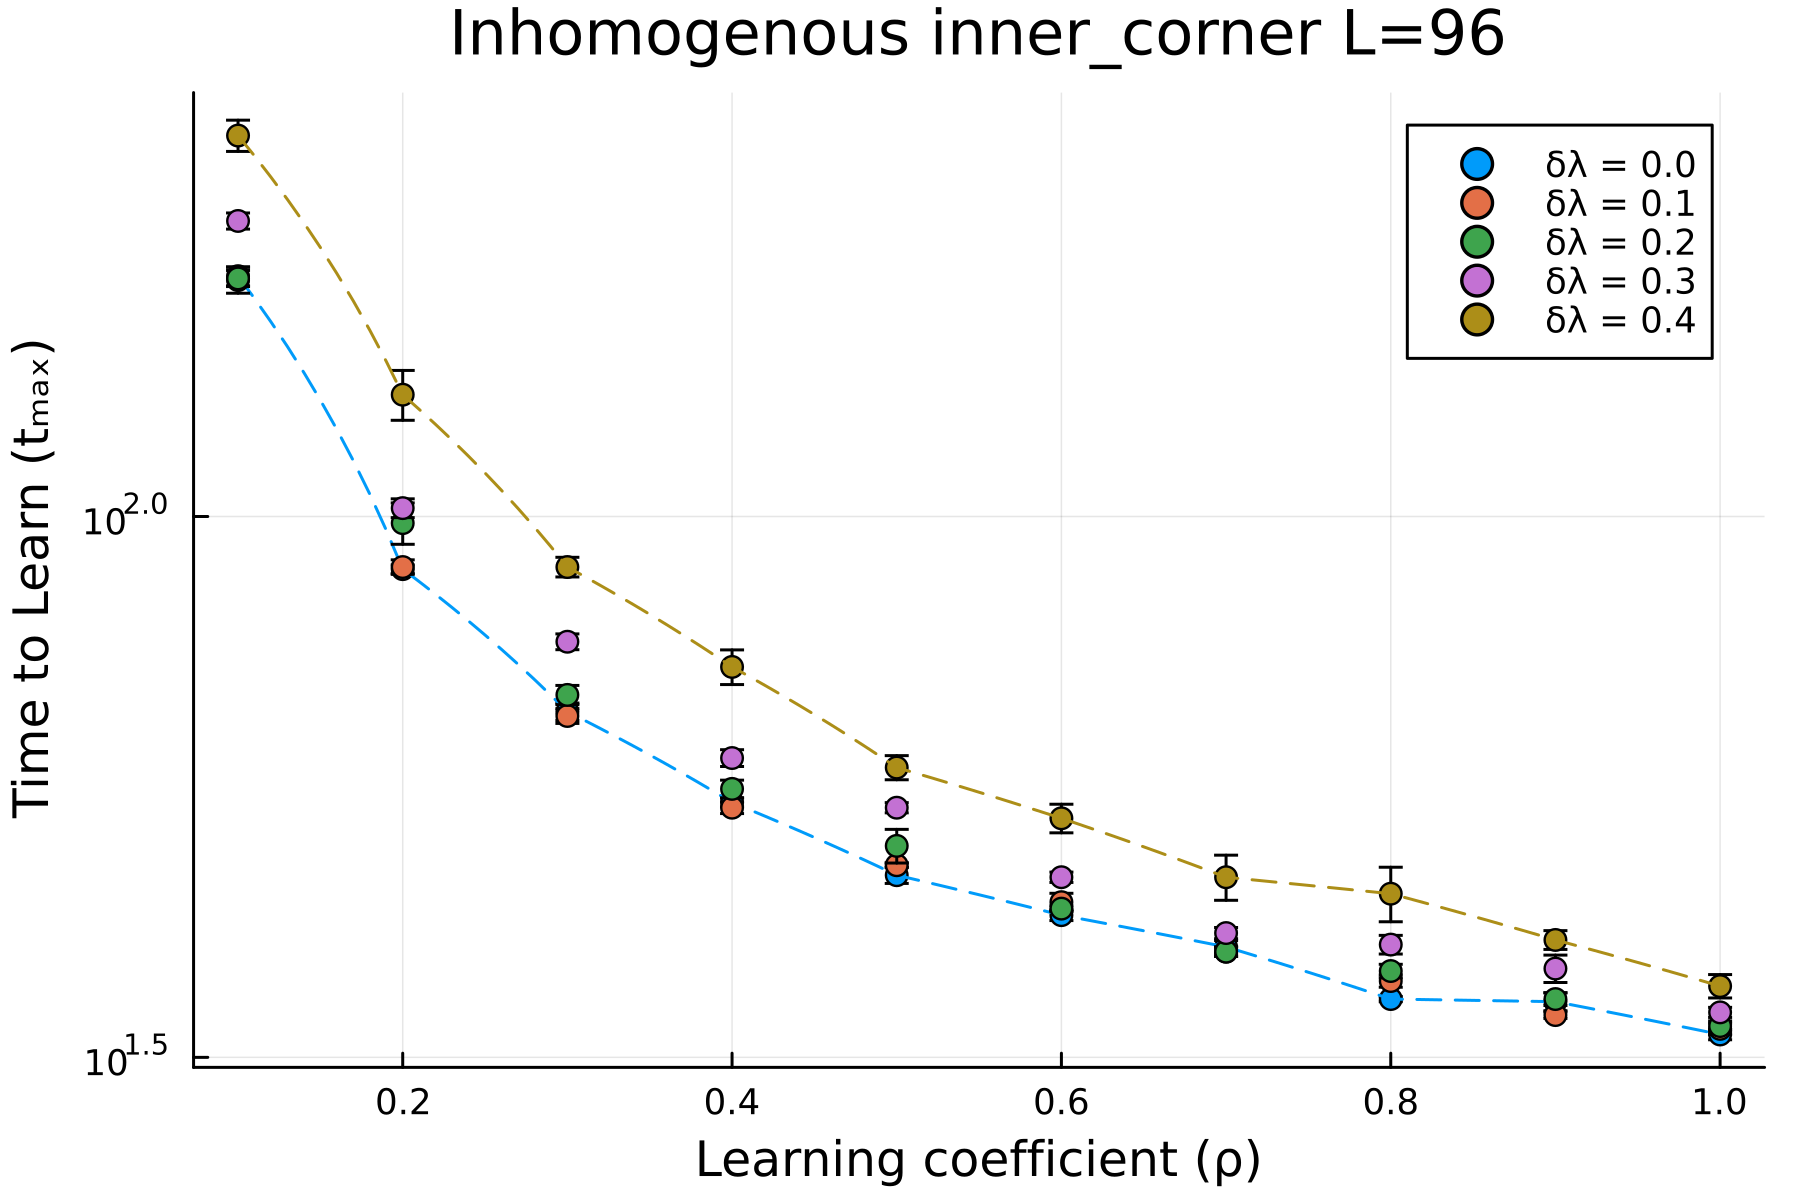
\includegraphics[width=0.49\textwidth]{figures/2D-BPCAIH-analysis/t-plots/t-inner_corner-96.png}}
   \subfigure[Traditional $L=48$]{\label{fig:2DBPCAIH t-rho plot T48}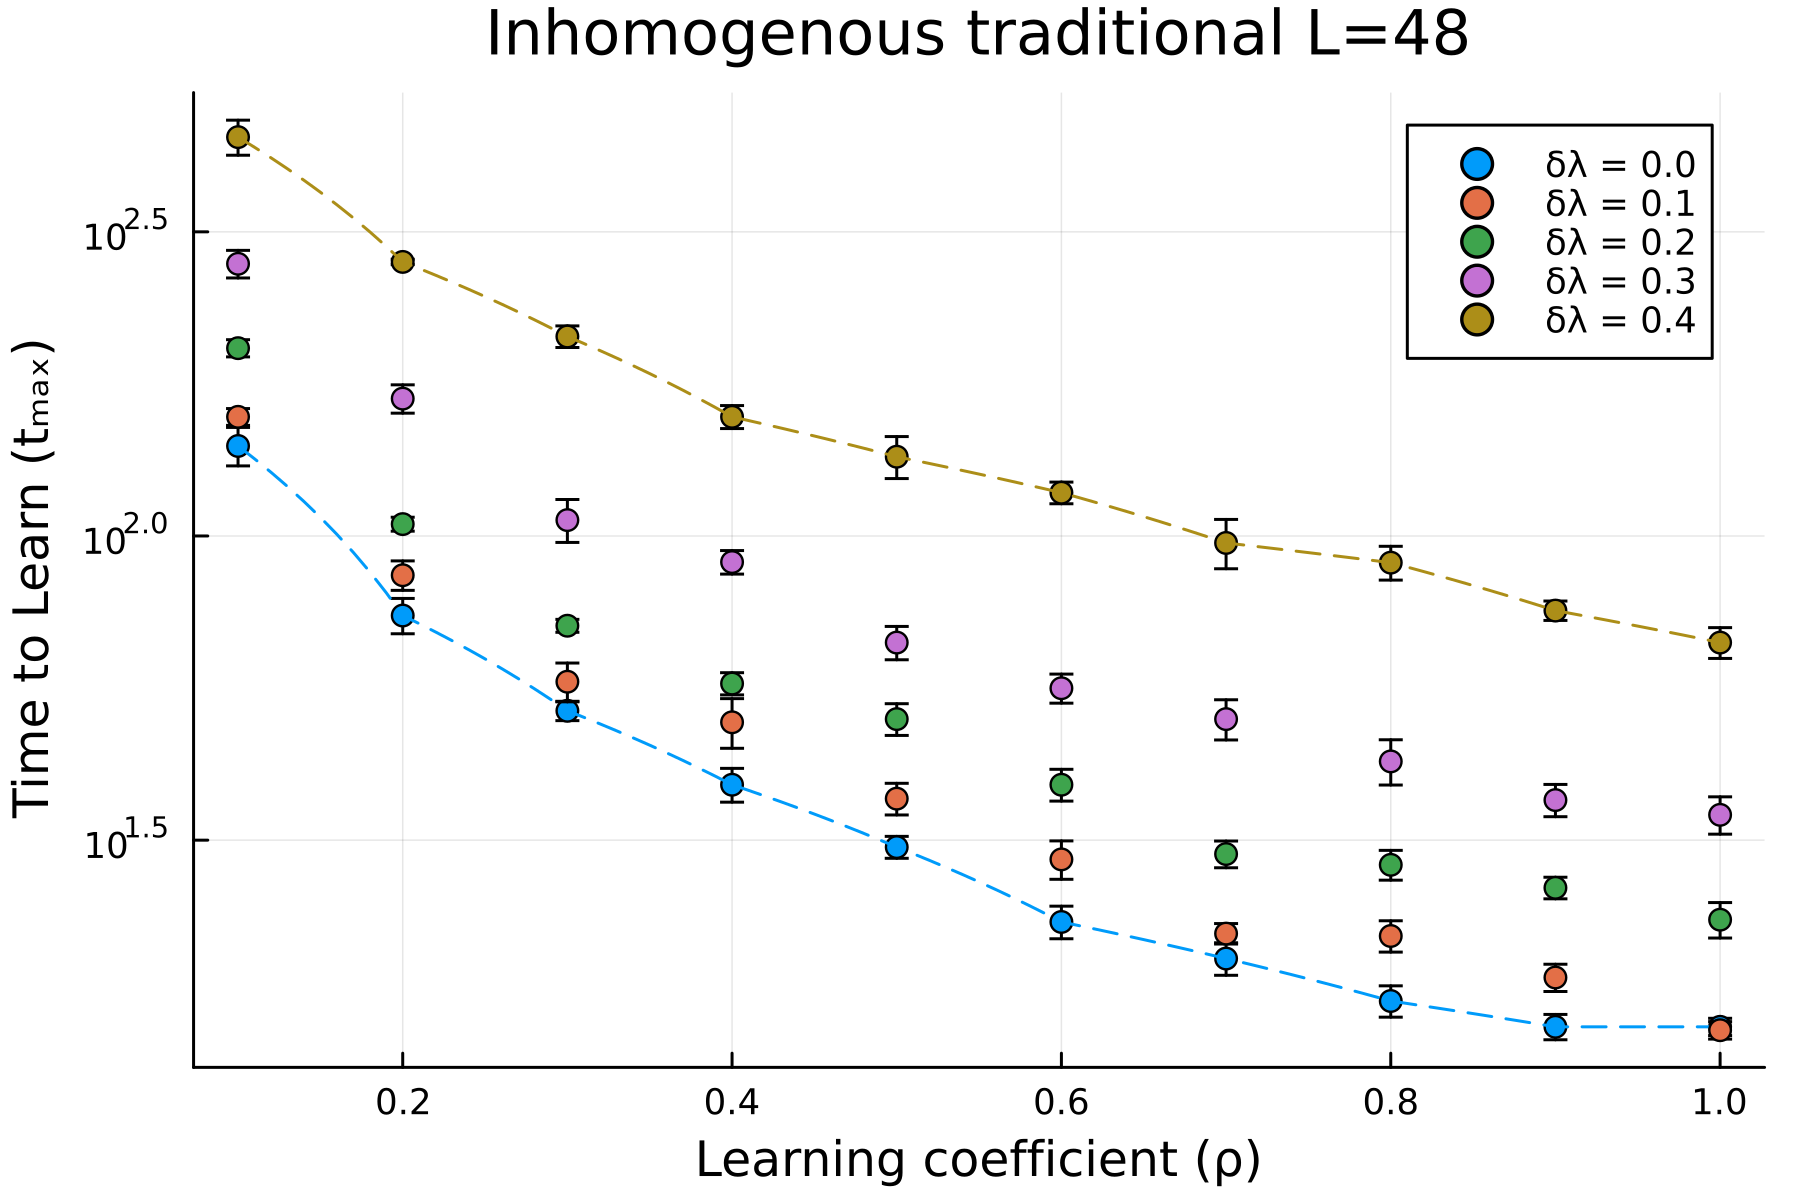
\includegraphics[width=0.49\textwidth]{figures/2D-BPCAIH-analysis/t-plots/t-traditional-48.png}}
   \subfigure[Traditional $L=96$]{\label{fig:2DBPCAIH t-rho plot T96}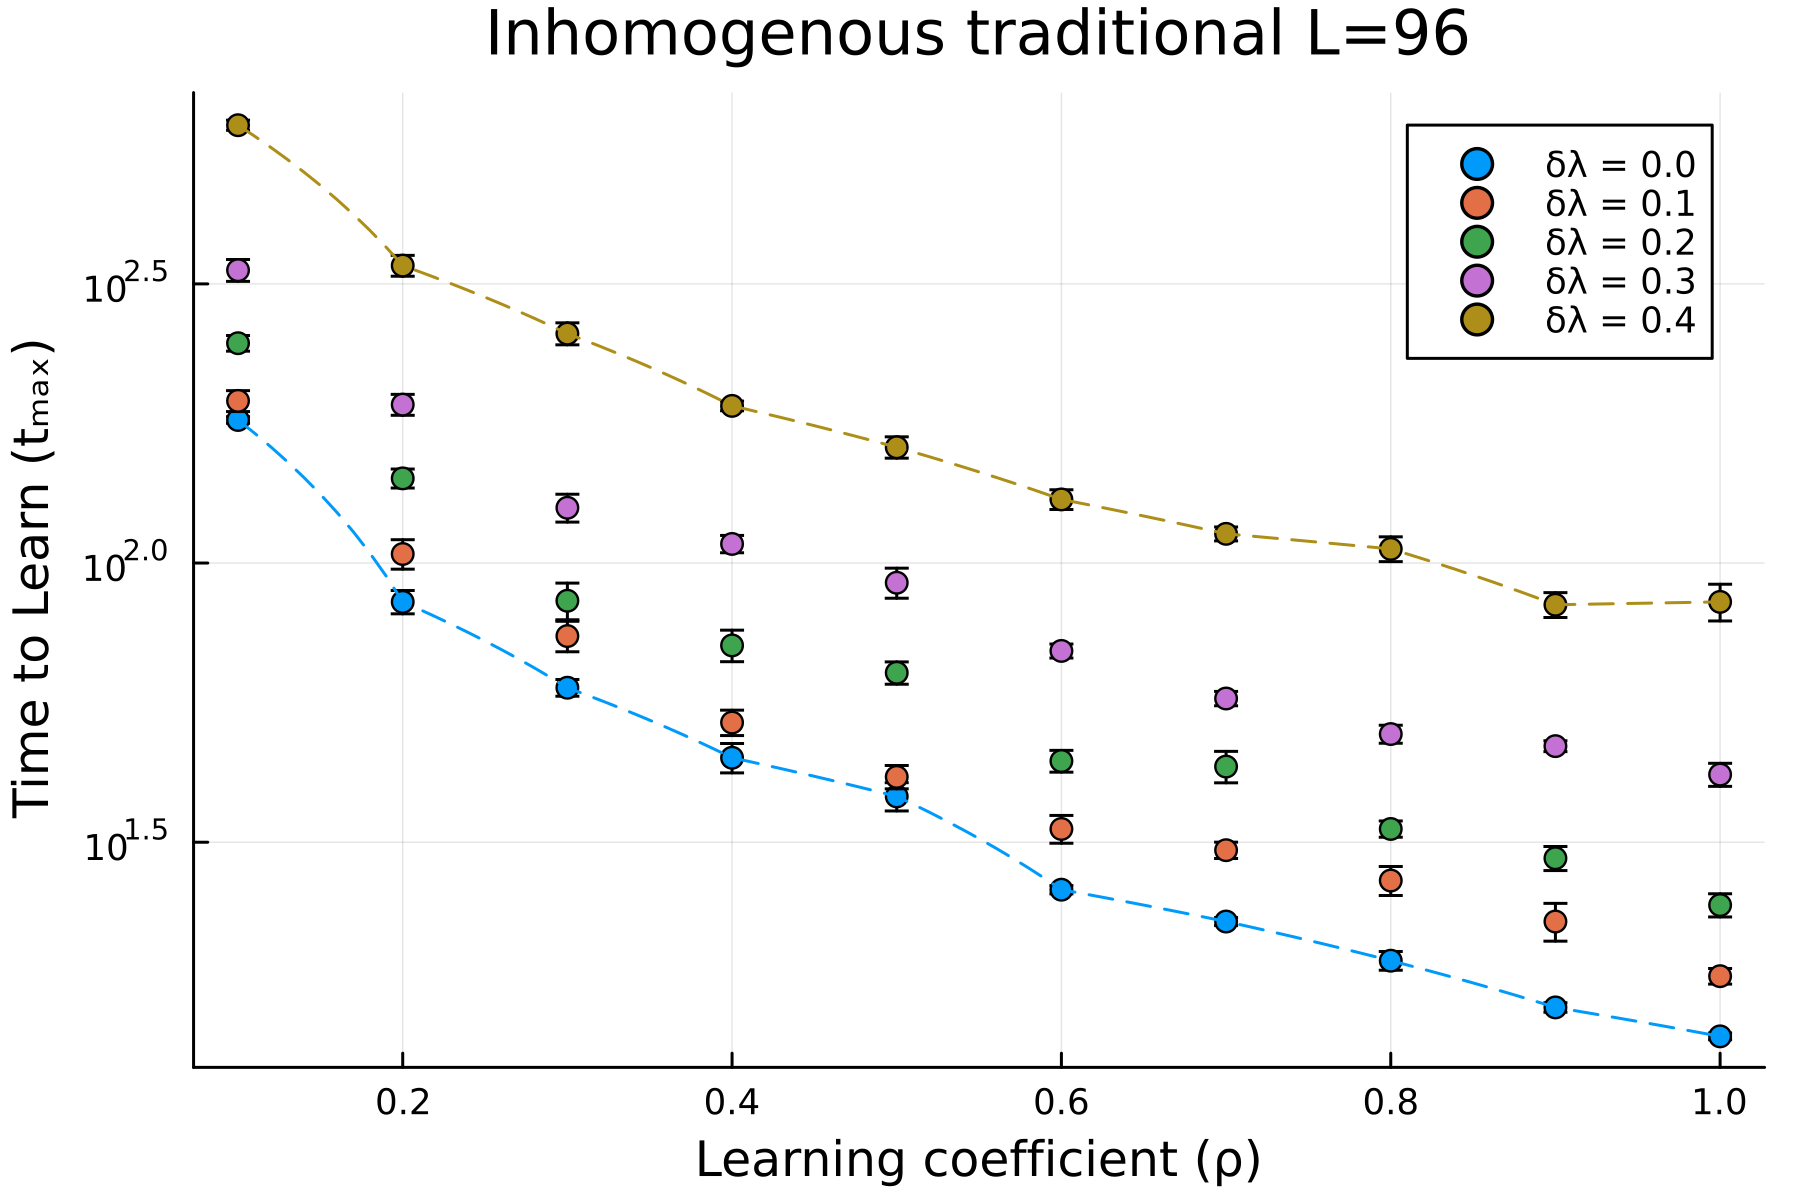
\includegraphics[width=0.49\textwidth]{figures/2D-BPCAIH-analysis/t-plots/t-traditional-96.png}}
   \caption{Time to learn $t_{max}$ as a function of positional learning factor $\rho_0$ for different representative classroom configurations and sizes with varying heterogeneity $\delta\lambda \in \lbrace 0, 0.1, 0.2, 0.3, 0.4 \rbrace$. Lower time to learn $t_{max}$ indicates better performance.}
   \label{fig:2DBPCAIH t-rho plot}
\end{figure}


\begin{figure}[htbp!]
   \centering
   \subfigure[$L=32$]{\label{fig:2DBPCAIH t-rho ribbon plot 32}\includegraphics[width=0.49\textwidth]{figures/2D-BPCAIH-analysis/rho-t ribbon plots/rho-t-ribbon-32.png}}
   \subfigure[$L=48$]{\label{fig:2DBPCAIH t-rho ribbon plot 48}\includegraphics[width=0.49\textwidth]{figures/2D-BPCAIH-analysis/rho-t ribbon plots/rho-t-ribbon-48.png}}
   \subfigure[$L=64$]{\label{fig:2DBPCAIH t-rho ribbon plot 64}\includegraphics[width=0.49\textwidth]{figures/2D-BPCAIH-analysis/rho-t ribbon plots/rho-t-ribbon-64.png}}
   \subfigure[$L=96$]{\label{fig:2DBPCAIH t-rho ribbon plot 96}\includegraphics[width=0.49\textwidth]{figures/2D-BPCAIH-analysis/rho-t ribbon plots/rho-t-ribbon-96.png}}
   \subfigure[$L=128$]{\label{fig:2DBPCAIH t-rho ribbon plot 128}\includegraphics[width=0.49\textwidth]{figures/2D-BPCAIH-analysis/rho-t ribbon plots/rho-t-ribbon-128.png}}
   \caption{Time to learn $t_{max}$ as a function of positional learning factor $\rho_0$ for the heteregenous model of all seating arrangements and classroom sizes $L$. 
   Each ribbon series represent the range of values for $t_{max}$ for a given seating arrangments with heterogeneity $\delta\lambda = \lbrace 0.0, 0.1, 0.2, 0.3, 0.4 \rbrace$.
   Lower time to learn $t_{max}$ indicates better performance.
   }
   \label{fig:2DBPCAIH t-rho ribbon plot}
\end{figure}

\newpage % new page after section t vs rho

\section{Time to learn $t_{max}$ vs heterogeneity $\delta\lambda$}\label{sec:BPCAIH t vs dl}

Figure~\ref{fig:2DBPCAIH dl-t plots} shows that as heterogeneity $\delta\lambda$ increases, PI methods perform better than traditional methods even when PI methods have lower positional learning factors $\rho_0$. For our represntative $\rho_0$ values, PI performs better than traditional methods regardless of the $\rho_0$ value, even in a large classroom $L=128$. 
However, in larger classrooms, the advantage in performance of PI over traditional methods is less pronounced. 
Furthermore, as class size increases, traditional methods tend to stay advantageous than PI methods for increasing values of heterge $\delta\lambda$.

For example, at $L=32$ shown in figure \ref{fig:2DBPCAIH dl-t plot 32}, PI methods are better than traditional methods for all values of $\delta\lambda$ when comparing between equal $\rho_0$ values. 
However, at $L=128$ shown in figure \ref{fig:2DBPCAIH dl-t plot 128}, the traditional model performs better than the PI model for $0 \leq \delta\lambda \leq 0.2$ when comparing between equal $\rho_0$ values.

\begin{figure}[htbp!]
   \centering
   \subfigure[$L=32$]{\label{fig:2DBPCAIH dl-t plot 32}\includegraphics[width=0.49\textwidth]{figures/2D-BPCAIH-analysis/dl-t plots/dl-t-32.png}}
   \subfigure[$L=128$]{\label{fig:2DBPCAIH dl-t plot 128}\includegraphics[width=0.49\textwidth]{figures/2D-BPCAIH-analysis/dl-t plots/dl-t-128.png}}
   \caption{Time to learn $t_{max}$ as a function of heterogeneity $\delta\lambda$ for the heteregenous models of the PI (inner corner SA) and traditional models with varying positional learning factor $\rho_0\in\lbrace 0.3,0.5,0.7 \rbrace$ and classroom sizes $L\in\lbrace32,128\rbrace$. 
   Each color represents a diffent value of $\rho_0$, while the circle and square symbols represent the traditional and PI models respectively.
   Lower time to learn $t_{max}$ indicates better performance.
   }
   \label{fig:2DBPCAIH dl-t plots}
\end{figure}

\newpage % new page after section t vs dl

\section{Time to learn $t_{max}$ vs class size $N$}\label{sec:BPCAIH m vs dl}

When investigating the size dependence of time to learn $t_{max}$ shown in Figure~\ref{fig:2DBPCAIH n-t plots}, we see a similar trend to what we found in section \ref{subsec: 2DBPCA tmax vs N} where PI models are better for smaller classes and traditional models are better for larger classes.
Heterogeneity $\delta\lambda$ generally has a negative effect on the time to learn $t_{max}$ for both PI and traditional models.
However, as shown in sections \ref{sec:BPCAIH t vs rho} and \ref{sec:BPCAIH t vs dl}, the traditional model is more affected by heterogeneity $\delta\lambda$ compared to PI models.
Because of the sensitivity of traditional instruction to heterogeneity $\delta\lambda$, at low values of $\rho_0$, even for large classes, PI models can perform better than traditional models for higher values of heterogeneity $\delta\lambda$.
This is shown in Figures \ref{fig:2DBPCAIH n-t plot 0.3} and \ref{fig:2DBPCAIH n-t plot 0.4} where the PI model performs better than the traditional model for all class sizes (N) and the same value of $\rho_0$.

\begin{figure}[htbp!]
   \centering
   \subfigure[$\delta\lambda=0.0$]{\label{fig:2DBPCAIH n-t plot 0.0}\includegraphics[width=0.49\textwidth]{figures/2D-BPCAIH-analysis/n-t plots/n-t-plot-0.0.png}}
   \subfigure[$\delta\lambda=0.1$]{\label{fig:2DBPCAIH n-t plot 0.1}\includegraphics[width=0.49\textwidth]{figures/2D-BPCAIH-analysis/n-t plots/n-t-plot-0.1.png}}
   \subfigure[$\delta\lambda=0.2$]{\label{fig:2DBPCAIH n-t plot 0.2}\includegraphics[width=0.49\textwidth]{figures/2D-BPCAIH-analysis/n-t plots/n-t-plot-0.2.png}}
   \subfigure[$\delta\lambda=0.3$]{\label{fig:2DBPCAIH n-t plot 0.3}\includegraphics[width=0.49\textwidth]{figures/2D-BPCAIH-analysis/n-t plots/n-t-plot-0.3.png}}
   \subfigure[$\delta\lambda=0.4$]{\label{fig:2DBPCAIH n-t plot 0.4}\includegraphics[width=0.49\textwidth]{figures/2D-BPCAIH-analysis/n-t plots/n-t-plot-0.4.png}}
   \caption{Time to learn $t_{max}$ as a function of class size $N$ for the heteregenous models of the PI (inner corner SA) and traditional models with varying positional learning factor $\rho_0\in\lbrace 0.1, 0.5, 0.9 \rbrace$ and heterogeneity $\delta\lambda\in\lbrace0.0, 0.1, 0.2, 0.3, 0.4 \rbrace$. 
   Each color represents a diffent value of $\rho_0$, while the circle and square symbols represent the traditional and PI models respectively.
   Each band represent the standard deviation of time to learn $t_{max}$ over 5 trials.
   Lower time to learn $t_{max}$ indicates better performance.
   }
   \label{fig:2DBPCAIH n-t plots}
\end{figure}

\newpage % new page after section t vs N



\section{Discussions/Conclusions?}\label{sec:BPCAIH discussions}
To better model the real world, we introduced heterogeneity to the students' learning rate. 
Adding heterogeneity does not affect the general trend of our instruction models. 
For the case of a heteregenous system, we still find traditional instruction fares better than PI for larger classes with high positional learning factor $rho_0$.

Besides not affecting the general trend, we also found out that traditional instruction is more sensitive to heterogeneity. 
As discussed in section \ref{sec:BPCAIH effects on classroom evolution}, the difference in sensitivity is because of the dynamics that were seen in the classes' evolution. 
This is related to the spatiotemporal dynamics of traditional learning models where the fast learning students learn first and the slow learning students learn last.
The time to learn $t_{max}$ for traditional instruction is then dependent on waiting for the slow students.

In contrast to the spatiotemporal dynamics of traditional instruction, the advantage of PI is that it is not as heavily dependent on the students themselves as traditional instruction.
PI is more dependent on the geomety of the classroom and the number of learning sources available to the students.
For the case of PI, the ``wavefront of learning'' (see: section \ref{sec:BPCAIH effects on classroom evolution}) provides students with more than one source of learning, unlike in the traditional model. 
This phenomenon offsets the increase in the time to learn $t_{max}$ that is caused by waiting for the slow learning students.
PI models therefore have a shorter time to learn $t_{max}$ despite being outperformed by the traditional model in earlier time steps.

Given the foregoing, initially performing traditional instruction and then proceeding with PI later would maximize each methods' strengths. 
The traditional instruction phase would yield high learning rates at the start of the simulation, by allowing the fast learning students to learn first.
The learned students would then be able to help the slow learning students learn in the PI phase, shortening the time to learn $t_{max}$.

% \begin{itemize}
%    \item PI models still better for small classrooms, traditional models better for large class sizes. Same for both homogenous and heterogenous.
%    \item heterogeneity can sway which set up is advantageous. Low heterogeneity favors traditional models, high heterogeneity favors PI models. Need to add plots for easier explanation.
%    \item Traditional models are more sensitive than heterogeneity. Higher difference, less effective traditional models.
%    \item Initial learning rate for traditional models is fast, but overall time to learn is longer than PI models. Natural consequence: trad then PI. This is what is done currently.
% \end{itemize}
 %%could be model or experiment set-up
% % !TEX root =  main.tex
\chapter{Mixed Model Instuction}

In this chapter, a sample for making equations and sub-equations
are demonstrated.

\section{Equations and sub-equations}

\hspace{\parindent} In the following, a set of equations is shown.
\begin{subequations}
\newcommand\del{\overrightarrow{\nabla}}
\begin{equation}\label{eq:EGauss}
    \del \cdot \vec{D} = \rho
\end{equation}
\begin{equation}\label{eq:BGauss}
    \del \cdot \vec{B} = 0
\end{equation}
\begin{equation}\label{eq:Faraday}
    \del \times \vec{E} = -\partial_t \vec{B}
\end{equation}
The last one being
\begin{equation}\label{eq:Ampere-Maxwell}
    \del \times \vec{H} = \vec{J} + \partial_t \vec{D}
\end{equation}
\end{subequations}
Note that text can still be placed between sub-equations within
the \verb+subequations+ environment.

When using a solitary equations, you may use the usual equation
syntax in \LaTeX.
\begin{equation}\label{eq:Maxwell}
    E = mc^2
\end{equation}
 %%could be results and discussions
% !TEX root =  main.tex
\chapter{Conclusion and Recommendations}
% \begin{itemize}
%     \item Traditional instruction is more scalable and is less dependent on class size.
%     \item PI performs better than traditional instruction in smaller classes with slower learners.
%     \item Among peer instruction setups, the inner corner seating arrangement is the most efficient.
%     \item Heterogeneity in students' learning rates can affect traditional instruction more than peer instruction.
%     \item traditional instruction would find themselves with two stages of learning: a fast initial stage and a slow final stage.
%     \item If instructors had to choose only one method, peer instruction would be the better choice. The advantage of PI over traditional instruction can be higher than the advantage of traditional instruction over PI.
% \end{itemize}

We proposed a probabilistic cellular automata model as a new way of investigating classroom learning dynamics.
We are able to investigate the effects of different factors governing two very different methods of instruction - traditional instruction and peer instruction (PI).

We found traditional instruction to be more scalable and less dependent on class size than PI.
On the one hand, the teacher is the only source of information in traditional instruction and is also able to teach all the students at the same time.
On the other hand, PI is more efficient in smaller classes because students have more sources of information (i.e. their seatmates). 
This offsets the simultaneous teaching advantage of traditional instruction.

We investigated different seating arrangements (SA) for PI and found that the inner corner SA is the most efficient setup from all SAs considered.
This optimal SA differs from a previous study where the outer corner SA is found to be the most efficient~\cite{roxas2010seating}.
The current model used in this work does not incorporate the effect of aptitude similarity~\cite{smith2009peer} between students in PI and isotropy in the learning direction.

To improve our model in reflecting real world factors, we also introduced heterogeneity in students' learning rates.
In doing this, it further emphasized one of the advantages of PI over traditional instruction - that PI is less affected by heterogeneity in students' learning rates.
In traditional instruction, the students with fast learning rates learn in the first few time steps, while the rest of the time it takes for the class to learn is waiting for the slow learners to learn.
This causes a two-stage learning process in traditional instruction.
The effect of heterogeneity in PI is less pronounced, only affecting the shape of the "wave of learning" but generally leaving the relevant trends and metrics unaffected.
These dynamics lead to PI performing better than traditional instruction in cases where class heterogeneity is high.
Additionally, we found that classes with slower learners, due to either the assigned positional learning factor $\rho_0$ or the learning rate $\lambda$, generally do better in PI than in traditional instruction.

Most previous studies focused on students' pre- and post-test scores to assess the advantages of PI over traditional instruction. 
That was not something we could do in this study because of the binary-state nature of our model.
However, we have confirmed results of experimental studies done before --- that PI can perform either similarly or better than traditional instruction \cite{crouch2001peer,lasry2008peer,thacker1994comparing,smith2009peer}.
We also found similar results regarding class heterogeneity --- that both methods of instruction are more effective with homogenous classrooms \cite{roxas2010seating}.

It is important to note that our model does not fully model the process of PI in real-world scenarios since it only models part of the PI process where students get to discuss the concept test questions with their seatmates.
We recommend that future researchers who want to delve deeper into this topic consider the effect of aptitude similarity in PI as described by Smith et al. (2009)~\cite{smith2009peer}.
Future works could also consider transitioning to a continuous-state model to better reflect real world situations.
Considering that our study suggests that the optimal method of instruction would be to have a short segment of traditional instruction followed by PI, which is similar to the actual process of PI in the classroom (i.e. reading and short lecture, concept test, sharing), future researchers who plan to model the classroom learning similarly should investigate the time delay between the two methods of instruction.
%% you may add more chapters by including more files just as above.
%% see the files for patterns of the format used.

\appendix
% !TEX root =  main.tex
\chapter{Appendix}

\section{Derivation of Equation \ref{eq:BPCA PI learning probability}} \label{sec: BPCA PI learning probability derivation}
\begin{subequations}
    For any event $e$, the desired outcome occurs with probability $p$ or not with probability $q$ where

    \begin{equation}
        \label{eq:A1}
        p + q = 1.
    \end{equation}

    \noindent For $n$ events, each being event $e$:
    \begin{equation}
        \label{eq:A2}
        \prod_{\forall e}(p_e + q_e) = 1.
    \end{equation}

    \noindent Expanding equation \ref{eq:A2}, we get
    \begin{equation}
        \label{eq:A3}
        \prod_{\forall e}{p_e}+ \ldots + \prod_{\forall e}{q_e} = 1.
    \end{equation}

    \noindent where the sum of the first $n-1$ terms is the probability of the desired outcome occurring at least once over $n$ events and the last term is the of the probability of the desired outcome not occurring at all. Thus, we can rewrite the probability of the desired outcome occurring at least once as

    \begin{equation}
        \label{eq:A4}
        P = 1 - \prod_{\forall e}{q_e}.
    \end{equation}

    \noindent substituting equation \ref{eq:A1} into equation \ref{eq:A4}, we get

    \begin{equation}
        \label{eq:A5}
        P = 1 - \prod_{\forall e}{(1 - p_e)}.
    \end{equation}
\end{subequations}

\section{Julia version packages used}
This study used \verb$Julia 1.11.0$ \cite{Julia-2017} with the following \verb$Julia$ packages and their hash codes:

% \begin{enumerate}
%     \item \verb$Alert.jl$ % can't find citation
%     \item \verb+CSV.jl+ % can't find citation
%     \item \verb$CairoMakie.jl$ 
%     \item \verb$ColorSchemes.jl$ % can't find citation
%     \item \verb$DataFrames.jl$ 
%     \item \verb$GLMakie.jl$ \cite{MakieJL}
%     \item \verb$LaTeXStrings.jl$ % can't find citation
%     \item \verb$LsqFit.jl$ % can't find citation
%     \item \verb$Measurements.jl$ \cite{Measurements.jl-2016}
%     \item \verb$Plots.jl$ \cite{PlotsJL}
%     \item \verb$ProgressMeter.jl$ % can't find citation
% \end{enumerate}

\begin{enumerate}
    \item \verb+Alert = "28312eec-4d86-447d-83ad-bc2b262de792"+
    \item \verb+CSV = "336ed68f-0bac-5ca0-87d4-7b16caf5d00b"+
    \item \verb+CairoMakie = "13f3f980-e62b-5c42-98c6-ff1f3baf88f0"+ \cite{MakieJL}
    \item \verb+ColorSchemes = "35d6a980-a343-548e-a6ea-1d62b119f2f4"+
    \item \verb+DataFrames = "a93c6f00-e57d-5684-b7b6-d8193f3e46c0"+ \cite{DataFramesJL}
    \item \verb+GLMakie = "e9467ef8-e4e7-5192-8a1a-b1aee30e663a"+ \cite{MakieJL}
    \item \verb+LaTeXStrings = "b964fa9f-0449-5b57-a5c2-d3ea65f4040f"+
    \item \verb+LsqFit = "2fda8390-95c7-5789-9bda-21331edee243"+
    \item \verb+Measurements = "eff96d63-e80a-5855-80a2-b1b0885c5ab7"+ \cite{Measurements.jl-2016}
    \item \verb+Plots = "91a5bcdd-55d7-5caf-9e0b-520d859cae80"+ \cite{PlotsJL}
    \item \verb+ProgressMeter = "92933f4c-e287-5a05-a399-4b506db050ca"+
\end{enumerate}

\section{Computer specifications and simulation time estimates}

\begin{itemize}
    \item CPU: Intel Core i7-10750H CPU
    \item Memory: 16 GB DDR4 RAM at 2933 MHz
    \item Storage: Samsung MZVLB1T0HBLR-000H1
    \item GPU: NVIDIA GeForce GTX 1650 Ti with Max-Q Design
    \item Operating system: Windows 11 Home Version 23H2
\end{itemize}

The simulation time estimates for the different scenarios are as follows:
\begin{itemize}
    \item Homogenous binary state PCA (1250 individual runs): 5 minutes
    \item Heterogeneous binary state PCA (6250 individual runs): 45 minutes
\end{itemize}

\section{GitHub repository}
The GitHub repository containing the codes and datasets used for the study can be found here: \url{https://github.com/ioakimsy/BS-Thesis}

\begin{figure}[h!]
    \centering
    \includegraphics[width=0.5\textwidth]{figures/qr-code.png}
    \caption{QR code for the GitHub repository}
    \label{fig:qr-code}
\end{figure}

% \hspace{\parindent}Include your codes when necessary to your
% thesis/dissertation. To do this, you may use \verb+verbatim+
% environment as follows. \textbf{WARNING:} All verbatim and
% verbatiminput environments should always be treated as a separate
% paragraph.  When included in a text paragraph, it sometimes happen
% to reduce the 1.5 spacing to the usual single-spaced text.

% {\small
% \begin{verbatim}
%  #include <iostream>
%  using std::cout;
%  using std::endl;

%  int main( void )
%  {
%     cout << "Hello world!" << endl;
%     return 0;
%  }
% \end{verbatim}
% }

% The \verb+{\small }+ bracketed region is used to lower the font
% size of the entire verbatim text.  This will save you much space
% and give a more aesthetical look in your manuscript.

% On the other hand, when very long codes are wished to be included
% automatically without the tedious cut and paste procedure, you may
% include them using the \verb+\verbatiminput+ command as follows.
% You may want to include a short description of the code of course.

% {\small
%  \verbatiminput{"codes/newC.cpp"}
% }

% This time, you may just include your recent codes by just
% copy-paste-ing the codes (as long they are clean!) into the
% directory \verb$codes/$ in the directory where this file is saved.


\bibliographystyle{ieeetr}
\bibliography{biblio} %% see file: "biblio.bib"

\end{document}
%%end of main.tex
